%% The World-Model Calculus — v3
%% A Sprout from the Formalization of PLN
%%
%% DESIGN PRINCIPLES:
%%   1. General WorldModel (revise, empty, extract — no laws) at the top
%%   2. Additive regime as the main exact specialization, not the whole theory
%%   3. Types from the start; Ch 8 deepens, Ch 4 introduces
%%   4. Evidence = generic conjugate carrier family
%%   5. Views are non-additive projections (proved)
%%   6. HOL/quantifiers used naturally where needed, not as "extensions"
%%   7. Finite prop Dirichlet is a worked fragment, not reference semantics
%%   8. Ch 2 is a self-contained overview of the entire theory
%%   9. Bio/genomics benchmarks in Part VI Applications
%%
%% Render: lualatex -shell-escape wm-pln-book_v3.tex

\documentclass[11pt,openany]{report}
\usepackage{pln-common}
\usepackage{tikz}
\usepackage{url}
\usetikzlibrary{arrows.meta,positioning,calc,decorations.pathreplacing}

\title{The World-Model Calculus\\[6pt]
  \large A Sprout from the Formalization of PLN\\[12pt]
  \normalsize\texttt{(v3 --- \today)}}
\author{Zar Goertzel \and Oru\v{z}i\thanks{%
  AI collaboration instantiated via
  Claude Opus~4.* (Anthropic),
  GPT-5.*~Pro (OpenAI),
  and Codex~5.* (OpenAI).}}
\date{}

\begin{document}
\maketitle
\tableofcontents


%% ═══════════════════════════════════════════════════════════════════
\part{Orientation and Overview}
\label{part:orientation}
%% ═══════════════════════════════════════════════════════════════════

\chapter{Introduction}
\label{ch:introduction}

\section{The Problem}

Any system that reasons under uncertainty must decide what to
store.  One family of answers---the one used by most PLN
implementations to date---stores \emph{truth values}: a strength
$s \in [0,1]$ and a confidence $c \in [0,1]$ attached to each
proposition.  Inference rules combine these pairs, producing new
truth values from old ones.

This works until you ask what happens when evidence arrives from
two sources that share a common cause, or when you need to retract
a faulty sensor's contribution, or when you want to explain
\emph{why} the system believes what it believes.  At that point,
the truth value is silent: it has already thrown away the structure
needed to answer.

The underlying issue is a conflation of three layers that should
be separate:
\begin{enumerate}
\item A \textbf{probabilistic world-model state}---the complete
  semantic object.
\item An \textbf{evidence algebra} for compositional
  aggregation---the carrier in which evidence lives.
\item \textbf{Operational truth-value views}---strength,
  confidence, intervals---which are derived summaries of the
  evidence, not the evidence itself.
\end{enumerate}
When these layers are collapsed into a single $(s, c)$ pair, the
result is what we call \emph{semantic drift}: algebraic operators
are treated as if they were the logic itself, and link-level
inference propagates correlation-sensitive quantities without
carrying the information required to do so correctly.

A one-line example makes the cost visible.  Consider two evidence
states: $e_1 = (1, 0)$ and $e_2 = (1, 1)$.  The second is more
\emph{informed} than the first---it contains strictly more
data---but less \emph{supportive} of the positive claim, because
the negative channel has increased.  A system that stores only
strength cannot distinguish ``strongly supported on little
evidence'' from ``weakly supported on much evidence.''  That
distinction is the subject of this book.


\section{The Move}

Replace truth values with \textbf{carried evidence state}.
The system stores sufficient statistics---not summaries---and
derives truth values as lossy projections (\emph{views}) only
when a decision must be made.

This is not a new idea.  It is what Bayesian statistics has always
done.  The contribution of this book is to make the move precise
for PLN-style uncertain reasoning, with eight normative
requirements (desiderata D1--D8, Chapter~\ref{ch:desiderata}),
a formal algebra, and machine-verified proofs.

Four verbs organize the calculus: \emph{revise} (incorporate new
evidence), \emph{query} (extract answers from the current state),
\emph{forget} (retract a source's contribution while preserving
the rest), and \emph{explain} (trace which evidence supports each
conclusion).  The next chapter presents the full calculus in
miniature.


\section{Four Distinctions}

Four distinctions recur throughout the book.  They are worth
stating here so the reader can watch for them:

\begin{description}
\item[State vs.\ view.]  The state is what the system carries
  (sufficient statistics, provenance, scope labels).  A view
  (strength, confidence, interval) is a lossy projection from
  the state.  Views are useful for display and thresholding;
  they are not proof objects.

\item[Semantics vs.\ compiled shortcut.]  The world model is the
  truthmaker.  A compiled rule (deduction, induction, abduction)
  is a certified shortcut that is exact under explicit side
  conditions.  When the conditions fail, the shortcut is not
  licensed.

\item[More information vs.\ more support.]  Evidence can improve
  in two senses that are not the same.  $(1, 1)$ is more informed
  than $(1, 0)$ but less supportive.  The book formalizes both
  orders and proves they are distinct
  (Chapter~\ref{ch:views}).

\item[Claim taxonomy.]  Every formal result in this book carries
  one of four labels:
  \claimCore{} (theorem-backed, no assumptions),
  \claimConditional{} (proved under declared assumptions),
  \claimBoundary{} (the claim is \emph{false} without its stated
  condition), or
  \claimOperational{} (heuristic or governance layer).
  Boundary results are among the most valuable: they tell you
  where not to waste effort.
\end{description}


\section{PLN Heritage}

This book grows out of the formalization of Probabilistic Logic
Networks~\cite{Goertzel2008PLN}.  The derived link calculus and
the compiled Bayesian-network constructions recover, sharpen, and
delimit classical PLN-style deduction, induction, and abduction
under explicit structural assumptions.

Where the original PLN rule family is correct, the present
calculus proves it correct and states the conditions.  Where it is
incomplete or semantically unstable, the present calculus states
the boundary and provides a typed, side-conditioned replacement.
The eight desiderata (Chapter~\ref{ch:desiderata}) are
requirements \emph{on} the calculus, not axioms \emph{of} it.
They come from lessons learned across PLN implementations---what
should have been true, and what went wrong when it was not.


\section{Maple Court}

\begin{figure}[htbp]
\centering
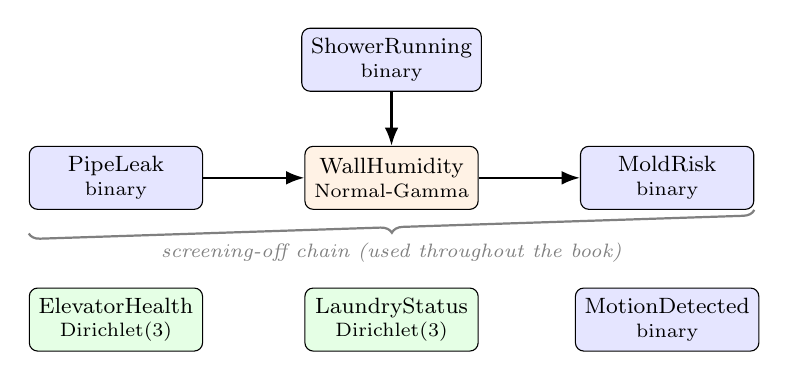
\begin{tikzpicture}[
  >=Latex,
  every node/.style={font=\footnotesize},
  bn/.style={draw, rounded corners=3pt, minimum width=22mm,
             minimum height=8mm, align=center},
  binary/.style={bn, fill=blue!10},
  dirichlet/.style={bn, fill=green!10},
  continuous/.style={bn, fill=orange!10},
]
  % Main chain (screening-off)
  \node[binary] (leak) at (0, 0) {PipeLeak\\[-1pt]\scriptsize binary};
  \node[continuous] (humid) at (3.5, 0) {WallHumidity\\[-1pt]\scriptsize Normal-Gamma};
  \node[binary] (mold) at (7, 0) {MoldRisk\\[-1pt]\scriptsize binary};
  \draw[->, thick] (leak) -- (humid);
  \draw[->, thick] (humid) -- (mold);

  % Collider: ShowerRunning also causes WallHumidity
  \node[binary] (shower) at (3.5, 1.5) {ShowerRunning\\[-1pt]\scriptsize binary};
  \draw[->, thick] (shower) -- (humid);

  % Independent nodes
  \node[dirichlet] (elev) at (0, -1.8)
    {ElevatorHealth\\[-1pt]\scriptsize Dirichlet$(3)$};
  \node[dirichlet] (laundry) at (3.5, -1.8)
    {LaundryStatus\\[-1pt]\scriptsize Dirichlet$(3)$};
  \node[binary] (motion) at (7, -1.8)
    {MotionDetected\\[-1pt]\scriptsize binary};

  % Label the chain
  \draw[decorate, decoration={brace, amplitude=4pt, mirror},
        thick, gray]
    (leak.south west) ++(0, -0.3) -- node[below=4pt,
    font=\scriptsize\itshape, text=gray]
    {screening-off chain (used throughout the book)}
    (mold.south east) ++(0, -0.3);
\end{tikzpicture}
\caption{The Maple Court building model.  Blue: binary evidence
  (alarm counts).  Orange: continuous evidence (Normal-Gamma
  sufficient statistics).  Green: categorical evidence (Dirichlet
  counts).  WallHumidity is a collider: both PipeLeak and
  ShowerRunning cause it.  The chain PipeLeak $\to$ WallHumidity
  $\to$ MoldRisk is the screening-off example used throughout.}
\label{fig:maple-court-bn}
\end{figure}

\maplecourt{%
Maple Court Community Commons is the book's running example.
Each apartment carries a private evidence state over questions
such as whether a pipe is leaking (binary: $(n^+, n^-)$ alarm
counts), whether the elevator is healthy (categorical: Dirichlet
counts over normal/slow/faulty), and what the hallway temperature
is (continuous: Normal-Gamma sufficient statistics).  Shared
spaces carry a building-level state.  Throughout the book, Maple
Court instantiates abstract concepts in teal-boxed asides like
this one.  All eight desiderata, all three primary carriers, and the
forgetting, provenance, and conservation theorems have Maple Court
examples.}


\section{Formal Verification}

The entire development is formalized in Lean~4 (version~4.28.0)
with Mathlib~v4.28.0.  The book-referenced files contain
hundreds of kernel-checked theorems with 0~sorry and 0~\code{native\_decide}
(Appendix~\ref{app:theorem-map}).  Six application domains---gas
sensor drift, steel fault classification, NAB anomaly detection,
GJP geopolitical forecasting, Bayesian-network inference, and
genomic hypothesis generation---have kernel-checked Lean fixtures.

This is not a decorative appendix.  It is the backbone.
Every ``Formalized in \ldots'' footnote in the text points to a
specific Lean file; a reader can build the file and verify the
claim in minutes.


\section{How to Read This Book}

The next chapter (Chapter~\ref{chap:overview}) presents the
entire calculus in miniature.  A reader who studies that chapter
will see how the whole book fits together before entering the
deeper technical development.  The remaining parts are:

\begin{description}
\item[Part~II] develops the calculus in depth: evidence
  carriers, state operations, views, and natively typed models.
\item[Part~III] covers compiled inference, Bayesian-network
  exactness, the no-go theorem, and large-scale inference control.
\item[Part~IV] extends to temporal, causal, and normative
  reasoning.
\item[Part~V] bridges to seven neighboring frameworks and states
  the limitations honestly.
\item[Part~VI] validates the framework on real benchmarks across
  six domains.
\end{description}

\noindent
This book is not a PLN tutorial or a replacement for the PLN
book.  It is a mathematical refoundation with formal
verification, aimed at researchers who want to understand PLN's
semantic commitments and extend the calculus to new domains.


\chapter{The World-Model Calculus: An Overview}
\label{chap:overview}

This chapter presents the world-model calculus in miniature.
It states the main semantic objects, the main exact regime, the
main boundary, and the role of typed structure and compiled
inference.  A reader who studies this chapter should see how the
whole book fits together before entering the deeper technical
developments.

\section{The Core Picture}
\label{sec:overview-core-picture}

At the highest level, the calculus has three typed parameters:
\[
  \textit{State}, \qquad \textit{Query}, \qquad V.
\]
A state is what the system currently carries.  A query is what the system may
ask.  The value type~$V$ is the carrier in which extracted answers live.  In
many applications $V$ will be a sufficient-statistic carrier such as binary
counts, Dirichlet counts, or Normal--Gamma statistics; in future work it may
also be probability-valued, interval-valued, or amplitude-valued.

The most general world-model interface records only three operations:

\begin{lstlisting}[language={}]
class WorldModel (State Query V : Type*) where
  revise  : State -> State -> State
  empty   : State
  extract : State -> Query -> V
\end{lstlisting}

This interface is intentionally minimal.  It says only that a world model is a
revisable state space equipped with query extraction.  No additivity,
commutativity, overlap law, or probabilistic interpretation is assumed at this
top level.  Those laws belong to later subclasses and later chapters.

The book works mostly in one especially important specialization: the
\emph{additive regime}.  There, state revision is additive, the value carrier is
an additive commutative monoid, and extraction commutes with additive
revision.  This is the regime in which the profile-hom equivalence,
Bayesian-network exactness theorems, provenance-tracked revision results, and
most of the current Lean development live.  But it is not presented as the
whole theory.  It is the main exact specialization of a broader family.

\maplecourt{Maple Court Community Commons is our running example.  Each
apartment carries a private posterior state over questions such as whether a
pipe is leaking, whether the shower is running, or whether motion indicates
occupancy.  Shared spaces carry a building-level state over hallway humidity,
laundry-room availability, and elevator health.  The same architecture appears
at both scales: revise the state as reports and sensor updates arrive, query the
state for evidence, and project that evidence into views only when a decision
must be made.}

\section{Revision Regimes and the Additive Powerhouse}
\label{sec:overview-regimes}

The calculus does not assume that all revision behaves the same way.  It is
useful to distinguish several regimes.

\begin{description}
\item[Additive revision.]  Independent or screening-off updates compose by
  addition.  This is the main tractable regime of the book.
\item[Overlap-aware revision.]  Two states may share information, so naive
  addition would double-count.  A correction or explicit overlap structure is
  required.
\item[Trust-gated revision.]  The merge operation depends on source trust or
  authority, so revision need not be symmetric or additive.
\item[Coalition or semitopological revision.]  Consensus is constrained by
  which coalitions are actionable; not every merge is valid.
\end{description}

Only the first of these is developed theoremically in full generality in the
present book.  The others already appear in the typed family and in the
formalization landscape, but they are treated as frontier directions rather than
as fully developed kernels.  Chapter~\ref{ch:world-models},
\S\ref{sec:non-additive} develops the \emph{non-additive perimeter}
in more detail: the overlap extraction law, semitopological coalitions,
and the recovery theorem showing that additivity is regained when
overlap is small or non-actionable ($\sim$60~theorems, 0~sorry).

The additive regime is captured by the following shape:

\begin{lstlisting}[language={}]
class AdditiveWorldModel (State Query V : Type*)
    [AddCommMonoid State] [AddCommMonoid V]
    extends WorldModel State Query V where
  revise_eq_add : forall W1 W2, revise W1 W2 = W1 + W2
  empty_eq_zero : empty = 0
  extract_add   : forall W1 W2 q,
    extract (W1 + W2) q = extract W1 q + extract W2 q
  extract_zero  : forall q, extract 0 q = 0
\end{lstlisting}

The decisive law is \code{extract\_add}.  It says that in the additive regime,
revising states and then extracting is the same as extracting first and then
combining answers in the carrier~$V$.  This is the exact algebraic condition
behind the cleanest part of the calculus.

\begin{theorem}[Additive answer-profile form]
\label{thm:overview-profile-hom}
For additive world models, currying the extractor yields an additive monoid
homomorphism
\[
  \widehat{\mathrm{extract}} : \textit{State} \to^+ (\textit{Query} \to V),
  \qquad
  W \mapsto (q \mapsto \mathrm{extract}(W,q)).
\]
Conversely, every additive monoid homomorphism
\(\textit{State} \to^+ (\textit{Query} \to V)\) determines an additive world
model.  Thus additive world models are exactly answer-profile generators.
\end{theorem}

This theorem is the categorical and algebraic center of the additive regime.
It says that, once additivity is assumed, a world model is one
structure-preserving arrow into an answer-profile object.  The extensional
model \(\textit{Query} \to V\) is terminal among additive world models over the
same query space: every additive world model maps canonically to its answer
profile.

This does \emph{not} trivialize the subject.  The hard work is in choosing
expressive state spaces, proving when compiled shortcuts are exact, and
showing where local summaries fail.  But it does make the kernel visible.

\section{Evidence Carriers}
\label{sec:overview-carriers}

Evidence is not one fixed datatype.  The general pattern is that a carrier
stores sufficient statistics for a conjugate family or other compositional value
system, and revision in the additive regime is addition of those sufficient
statistics.

In the current development three carriers are central.

\begin{description}
\item[Binary evidence.]  A two-channel carrier recording positive and negative
  support.  This is the historical PLN carrier, now treated as one instance
  among others.
\item[Dirichlet evidence.]  A multi-valued carrier recording category counts.
  This is the right instance for questions with more than two alternatives.
\item[Normal--Gamma evidence.]  A continuous-domain carrier storing the
  sufficient statistics needed for unknown mean and variance.
\end{description}

In Maple Court these arise naturally.  Leak alarms and motion detections are
binary.  Elevator health and laundry status are multi-valued.  Hallway
humidity and temperature are continuous.  The calculus does not change across
these cases; only the carrier does.

The additive regime explains why revision is so simple in these families:
counts add, sufficient statistics add, and the extractor commutes with that
addition.  Some additional algebraic structure can then be studied on top of
particular carriers.  For binary evidence, the current development includes a
quantale tensor and a Heyting structure.  Those are mathematically real, but
they were originally developed for binary evidence but have now
been extended to the full $k$-ary Dirichlet family:
coordinatewise multiplication gives a commutative monoid tensor,
and the lattice gives a complete Heyting algebra (Frame) for all
$k$, not just $k = 2$.%
\footnote{Formalized in
\codepath{Mettapedia/Logic/EvidenceDirichletQuantale.lean}
(13~theorems, 0~sorry).  The round-trip at $k=2$ recovers
\code{BinaryEvidence} exactly.}

Evidence items also carry an \emph{epistemic kind} label
(empirical, expert-elicited, model-derived, text-interpreted,
logically derived) that records where the evidence came from.
The same pseudo-count means different things depending on whether
it arose from sensor data or expert judgment
(Chapter~\ref{ch:state-ops}).  When conjugacy holds, sufficient
statistics are lossless compressions of the raw observations; the
raw data can optionally be retained for model switching, auditing,
or distributional queries that exceed the carrier's resolution.


\section{States Are Primary: Revise, Query, Forget, Explain}
\label{sec:overview-four-verbs}

The book revolves around four verbs:
\emph{revise}, \emph{query}, \emph{forget}, and \emph{explain}.

Revision and querying are the minimal kernel operations.  Forgetting and
explanation show why the kernel stores states rather than floating truth values.
A state can be updated, partially retracted, audited, replayed, and explained in
a way that a naked scalar view cannot.

\maplecourt{Suppose three hallway humidity alerts arrive, then one sensor is
found to be faulty.  If the system carries only a strength estimate such as
$0.83$, it is unclear how to retract just the faulty source.  If the system carries
a revisable state with provenance, forgetting can remove the appropriate
contribution while preserving answers outside the forgotten scope.  The same
state can also explain why the building robot now believes the hallway needs
mopping: not because the confidence number crossed an arbitrary threshold in
the abstract, but because specific reports and sensors revised the building
state in a tracked way.}

This is why provenance is not ``mere metadata.''  It is part of the structure of
stateful reasoning.  Likewise, forgetting is not an optional convenience.  It is a
semantic operation that clarifies what kind of proof object a world-model
state really is.

\section{Information, Support, and Views}
\label{sec:overview-views}

One of the deepest distinctions in the book is that evidence can improve in
more than one sense.  It can become \emph{more informed}, and it can become
\emph{more supportive} of a query.  These are not the same order.

For binary evidence, compare
\[
  e_1 = (1,0),
  \qquad
  e_2 = (1,1).
\]
The second state is more informative than the first in the ordinary
information-order sense: it contains at least as much positive and at least as
much negative evidence.  But it is less supportive of the positive claim,
because the negative channel has increased as well.  A strength view therefore
decreases even as total evidence increases.

This distinction drives the architecture.

\begin{proposition}[Views are not additive semantics]
\label{prop:overview-views-not-semantic-core}
In the current development, total evidence is additive, but central operational
views such as strength are not.  More generally, useful readouts from evidence
may be informative, calibrated, or decision-relevant without preserving the
revision law of the underlying carrier.
\end{proposition}

So a view is not a proof object.  It is a projection.  This is why the book keeps
views after evidence and state operations, not before them.  The semantics lives
in state and extraction; views are derived interfaces for display, thresholding,
and action.

\section{Natively Typed World Models}
\label{sec:overview-typed}

The calculus is typed from the beginning.  Its primary sorts are already
visible in the kernel:
\[
  \textit{State}, \qquad \textit{Query}, \qquad V.
\]
What later chapters develop in more detail is not a second semantics but a
full native typed realization of the same calculus: a rewrite family whose
terms, rules, and native types expose the same mathematical structure from
inside.

In the additive regime, the core rewrite system is organized by a
$2 \times 2$ calculus square: raw versus guarded, and plain versus
congruence-aware.  Later chapters expand this to a richer typed
family, prove the encoding is biconditionally adequate (the typed
and algebraic presentations agree exactly), and show that for any
type~$T$, multiset ensembles give a canonical world
model---suggesting the framework may be universal for typed
rewrite systems (Chapter~\ref{ch:typed}).

Logical structure appears wherever the query space carries it.  Quantified and
higher-order queries are not presented as ``extensions'' to a lower theory.
They are simply instances of the general \textit{Query} parameter when one wants
logical structure rich enough to express those questions.

\section{Compiled Inference and the PLN Connection}
\label{sec:overview-compiled}

The calculus does not treat deduction, induction, and abduction as primitive
truth-value algebra.  It treats them as \emph{compiled rewrites}: certified
shortcuts that are exact under explicit side conditions within declared model
classes.

This is where the book most visibly overlaps with the PLN tradition.  The
derived link calculus and the compiled Bayesian-network rules formalize,
sharpen, and delimit the classical PLN rule family.  The point is not to deny
that those rules can be useful.  The point is to state exactly when they are
correct, what they compute, and what they leave out.

\maplecourt{Suppose the building model contains the chain
\(\textit{PipeLeak} \to \textit{WallHumidity} \to \textit{MoldRisk}\).
A maintenance agent wants to answer a leak-related query quickly.  Rather
than recomputing the full posterior from scratch, the system may use a
compiled chain rule justified by the BN factorization and screening-off
assumptions attached to that model class.  When those side conditions hold,
the compiled answer agrees with the full extractor on the covered query
family.  When they do not hold, the rewrite is not licensed.}

That is the modernized meaning of a PLN rule inside WM-PLN:
not a free-standing law of truth values, but a typed and side-conditioned
shortcut to a result already determined by the underlying world model.
The most exact form of chaining propagates the \emph{full posterior
distribution} through the chain, not just scalar strength and
confidence.  Five certified-chaining limitation theorems
(Chapter~\ref{ch:error-transport}) make the cost of the scalar
approximation precise.  Demand-directed backward chaining
(Chapter~\ref{ch:scale-control}) complements forward supply:
demand propagation identifies which premises are most worth
investigating, and the demand contracts after supply fills the
information gap.

\section{The Boundary: Why Local Chaining Cannot Be Complete}
\label{sec:overview-boundary}

The book's main negative result explains why compiled inference must be
handled so carefully.

\begin{theorem}[No-go for unrestricted local link completeness]
\label{thm:overview-no-go}
In general, complete link evidence cannot be recovered from local per-link
surrogates alone.  Two world-model states can agree on all chosen local link
summaries while differing on the complete evidence needed for the target
query.
\end{theorem}

This boundary theorem is not an embarrassment.  It is a design theorem.  It
says that unrestricted local chaining cannot replace a complete semantics.  It
also explains why structural side conditions matter so much: compiled shards
become exact only inside model classes that carry enough global structure for
those shortcuts to commute with full extraction.

The no-go theorem is also one reason the non-additive frontier matters.  When
sources overlap, correlations matter, or trust gates revision, naive local
summary propagation is even less likely to preserve the required structure.
The additive regime is powerful precisely because it identifies a large,
tractable class in which the profile-hom story, carrier algebra, and compiled
rules all fit cleanly together.

\section{A Compact End-to-End Picture}
\label{sec:overview-end-to-end}

The overview can now be summarized in one pipeline:

\medskip
\noindent
\makebox[\textwidth][c]{%
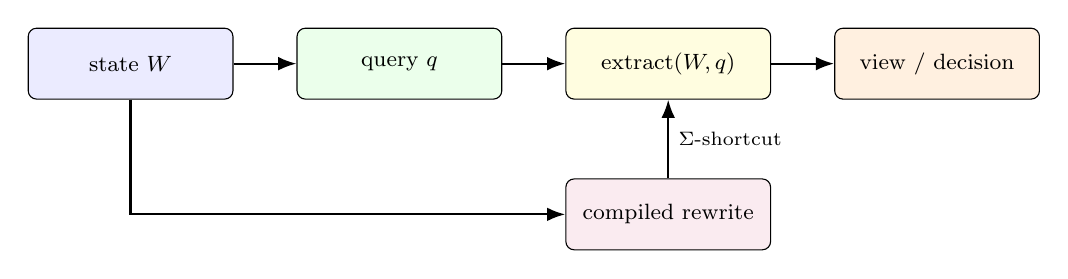
\begin{tikzpicture}[
  >=Latex,
  every node/.style={font=\footnotesize},
  box/.style={draw, rounded corners=3pt, minimum width=26mm,
              minimum height=9mm, align=center}
]
  \node[box, fill=blue!8] (state) {state $W$};
  \node[box, fill=green!8, right=8mm of state] (query) {query $q$};
  \node[box, fill=yellow!12, right=8mm of query] (extract) {extract$(W,q)$};
  \node[box, fill=orange!12, right=8mm of extract] (view) {view / decision};
  \node[box, fill=purple!8, below=10mm of extract] (rewrite) {compiled rewrite};

  \draw[->, thick] (state) -- (query);
  \draw[->, thick] (query) -- (extract);
  \draw[->, thick] (extract) -- (view);
  \draw[->, thick] (state) |- (rewrite);
  \draw[->, thick] (rewrite) -- node[right, font=\scriptsize]
    {$\Sigma$-shortcut} (extract);
\end{tikzpicture}}
\medskip

The state is primary.  Queries interrogate the state.  Extraction returns values
in a carrier.  Views project from those values.  Compiled rewrites accelerate
families of queries under explicit side conditions.  Boundaries tell us where
such shortcuts cannot be complete.

The computational story is layered: revision is $O(1)$ (add
sufficient statistics); single-query extraction is $O(1)$; but
full joint inference over many correlated queries is as hard as
the underlying model class (\#P-hard for general Bayesian
networks).  The calculus does not make this cheaper.  What it does
is make the cost \emph{visible}: the $\Sigma$-guard tells you
exactly which queries admit cheap compiled shortcuts, the no-go
theorem tells you which do not, and the demand layer tells you
where to spend your computational budget.

That is the whole book in compressed form.

\section{What the Calculus Does in Practice}

The applications (Part~\ref{part:applications}) test the
calculus on real data: gas sensor drift across 36~months
(governance question: when to retrain?), geopolitical forecast
aggregation (forgetting stale reliability weights improves
prediction), Bayesian-network benchmarks (distributional inference
reduces MAE by $1.5$--$3.8\times$), and eight PPLBench lanes
(matching Stan's posteriors at $O(1)$ per update).  The empirical
contribution is not raw accuracy but inference-control quality:
exact where licensed, bounded where partially licensed, abstaining
where not.

\section{How the Rest of the Book Unfolds}
\label{sec:overview-rest}

The remaining chapters slow this compact picture down.
Part~II develops the algebra and its instances in full.
Part~III formalizes compiled inference, BN exactness, and
large-scale inference control.
Parts~IV--V extend to temporal, causal, and normative reasoning,
bridge to seven neighboring frameworks, and state the limitations
honestly.
Part~VI validates the framework empirically across six domains.

The intended reading experience is two-layered.  This overview
shows the crystal.  The rest of the book turns the crystal in the
light, proves its faces, and follows each face into deeper
mathematics and larger applications.

\paragraph{PLN heritage.}
The relationship of this material to the PLN
tradition---what it recovers, what it corrects, what it
delimits---is discussed in the Introduction
(Chapter~\ref{ch:introduction}).


\chapter{Desiderata}
\label{ch:desiderata}

Before building the calculus, we state what it must achieve.  This
chapter lists eight normative requirements---\emph{desiderata}---that
the design is held accountable to.  Each desideratum is stated as a
named, numbered property so that later chapters can cite it explicitly
when discharging it.  The desiderata are not axioms of the calculus
(those come in Chapter~\ref{ch:world-models}).  They are requirements
\emph{on} the calculus: properties that a well-designed framework for
uncertain reasoning ought to satisfy, and that we claim this one does
satisfy, under conditions that will be made precise.

\paragraph{Why desiderata, not axioms?}
An axiom is a starting point for derivation.  A desideratum is a
target for design.  The distinction matters because several of the
properties below are not simultaneously achievable in full generality:
the no-go theorem (Chapter~\ref{ch:no-go}) shows that local chaining
cannot be universally complete, and the five chaining-limitation
theorems (Chapter~\ref{ch:error-transport}) show that scalar
propagation inevitably loses information.  The desiderata say what
we \emph{want}; the theorems say what we \emph{get} and where we
\emph{stop}.  The interplay between the two is what gives the book
its shape.

\paragraph{Origin.}
These desiderata crystallized during the formalization of Probabilistic
Logic Networks~\cite{goertzel2009pln}.  The original PLN design
implicitly assumed most of them---evidence-based reasoning, the
strength-confidence decomposition, revision as evidence combination,
the idea that inference rules are derived rather than primitive.  What
PLN v0.9 did not do was state these requirements explicitly, prove them
under typed conditions, or delineate where they fail.  The present list
makes the implicit contract explicit.

\paragraph{Independence.}
The eight desiderata are logically independent: for each one, there
exists a system satisfying the other seven while violating it.  These
independence witnesses are noted after each statement.  The
independence claim is not a theorem of the formal development---it is a
design observation that justifies each desideratum's inclusion as
non-redundant.

\bigskip

The desiderata are organized in three layers.  The first two
(\textbf{D1}--\textbf{D2}) define the semantic kernel.  The next two
(\textbf{D3}--\textbf{D4}) constrain the evidence architecture.
The final four (\textbf{D5}--\textbf{D8}) constrain inference,
retraction, conservation, and self-knowledge.

\maplecourt{%
Each desideratum will be illustrated with Maple Court's building
model.  The illustrations are not proofs---they are concrete
instances showing that the desiderata arise naturally in a realistic
evidence-management scenario, not as abstract stipulations.}


%% ═══════════════════════════════════════════════════════════════
\section{D1: State Primacy}
\label{sec:d1}
%% ═══════════════════════════════════════════════════════════════

\begin{definition}[Desideratum D1 --- State Primacy]
\label{def:d1}
A reasoning system should carry a \emph{revisable state} that can be
updated, queried, partially retracted, and explained.  Truth-value
summaries are derived from states, never stored as the primary
representation.
\end{definition}

\noindent
The philosophical motivation is elementary: a bare number has no parts.
You cannot ask \emph{where} a strength of $0.83$ came from, which
observations contributed to it, or what would happen if one source were
retracted.  A state has structure.  It records what was observed, by
whom, and when.  The four verbs of the calculus---revise, query,
forget, explain---all require state; the first two require it
minimally, the last two require it essentially.

\paragraph{What D1 rules out.}
Any system that stores only a scalar summary (a probability, a
strength-confidence pair, a log-odds value) as its primary
representation violates D1.  Classical probability calculus violates D1
when probabilities are treated as fundamental rather than derived from
evidence.  PLN v0.9 satisfies D1 in spirit (it carries evidence
counts) but does not formalize the state operations that D1 enables
(forgetting, explanation).

\paragraph{Discharge.}
D1 is discharged by the \code{WorldModel} typeclass
(Chapter~\ref{ch:world-models}), which takes $\mathrm{State}$ as a
first-class typed parameter with \code{revise}, \code{empty}, and
\code{extract} as operations.

\paragraph{Independence witness.}
A lookup-table system that maps queries directly to real-valued
answers (no state, no revision) satisfies D2--D8 trivially but
violates D1: there is nothing to revise, retract, or explain.

\maplecourt{%
Each Maple Court apartment carries a private state over questions such
as ``Is there a pipe leak?'' and ``Is the shower running?''  The state
is not the strength $0.83$---it is the evidence pair $(5, 1)$: five
leak alarms and one no-alarm reading.  The state can be revised
(a new alarm arrives), queried (what is the current leak evidence?),
forgotten (retract the reading from the miscalibrated sensor), and
explained (the evidence came from sensors 3B-north and 3B-south,
installed on 2025-01-15).}


%% ═══════════════════════════════════════════════════════════════
\section{D2: Compositional Extraction}
\label{sec:d2}
%% ═══════════════════════════════════════════════════════════════

\begin{definition}[Desideratum D2 --- Compositional Extraction]
\label{def:d2}
In the primary regime, querying a revised state should decompose into
queries of the components:
\[
  \mathrm{extract}(\mathrm{revise}(W_1, W_2),\, q)
  = \mathrm{combine}(\mathrm{extract}(W_1, q),\;
                       \mathrm{extract}(W_2, q)).
\]
That is, extraction should be a homomorphism from the state monoid to
the value monoid.
\end{definition}

\noindent
This is the algebraic heart of the additive regime.  It says that
evidence from independent sources can be combined without interference:
the result of revising and then querying equals the result of querying
each source separately and then combining the answers.

\paragraph{Why this matters.}
Compositional extraction is what makes the profile-hom equivalence
(Theorem~\ref{thm:universal-property}) possible: an additive world
model \emph{is} a monoid homomorphism from states to answer profiles.
Without compositionality, there is no universal property, no clean
categorical picture, and no guarantee that compiled inference shortcuts
agree with full extraction.

\paragraph{The foundational justification.}
D2 is not an arbitrary algebraic choice.  De~Finetti's representation
theorem for exchangeable sequences shows that, under exchangeability,
sufficient statistics add: $(n_1^+, n_1^-) + (n_2^+, n_2^-) =
(n_1^+ + n_2^+, n_1^- + n_2^-)$.  The Solomonoff--de~Finetti
foundation (Chapter~\ref{ch:world-models}, \S``The Solomonoff--De
Finetti Foundation'') establishes the categorical necessity chain:
%
\begin{center}
\begin{tabular}{@{}c@{}}
exchangeability $\to$ de~Finetti mixture $\to$ Kyburg flattening \\
$\to$ Giry bind $\to$ evidence sufficiency.
\end{tabular}
\end{center}
%
\noindent
D2 is the algebraic shadow of this necessity.

\paragraph{What D2 rules out.}
Any system whose query answers depend on the \emph{order} of evidence
arrival (in the independent-sources case) violates D2.  Classical
Bayesian updating satisfies D2 at the level of sufficient statistics
but violates it at the level of posterior probabilities (normalization
destroys additivity).  This is exactly why the calculus operates on
carriers (sufficient statistics), not on probabilities.

\paragraph{What D2 does not require.}
D2 is stated for the ``primary regime'' (the additive regime).  It is
\emph{not} required for all revision modes.  The overlap-aware,
trust-gated, and coalition regimes of Chapter~\ref{ch:world-models}
explicitly violate D2, and this is expected: when sources share
information, or when trust gates revision, naive composition is wrong.
D2 identifies the regime where composition is exact; the other regimes
are frontier directions where D2's algebraic convenience is traded for
richer structure.

\paragraph{Discharge.}
D2 is discharged by the \code{AdditiveWorldModel} axiom
\code{extract\_add} (Chapter~\ref{ch:world-models},
\S\ref{sec:additive-regime}) and the profile-hom equivalence
(Theorem~\ref{thm:universal-property}).

\paragraph{Independence witness.}
A system that carries states and supports forgetting (D1, D6) but
uses a nonlinear extraction---e.g.,
$\mathrm{extract}(W_1 + W_2, q) = \max(\mathrm{extract}(W_1, q),
\mathrm{extract}(W_2, q))$---satisfies D1, D3--D8 but violates D2.

\maplecourt{%
Apartment~3B receives two independent sensor reports about the pipe:
$(3, 1)$ from the north sensor and $(2, 0)$ from the south sensor.
D2 says the combined evidence is $(5, 1)$, the same whether we
combine first and then query, or query each and combine the answers.
The order of arrival does not matter; the combination is commutative
and associative.  This is why the apartment can buffer overnight
readings and batch-update at dawn (the sleep-consolidation theorem,
Theorem~\ref{thm:sleep-consolidation}).}


%% ═══════════════════════════════════════════════════════════════
\section{D3: Generic Evidence Carriers}
\label{sec:d3}
%% ═══════════════════════════════════════════════════════════════

\begin{definition}[Desideratum D3 --- Generic Carriers]
\label{def:d3}
The value type $V$ in which extracted answers live should be a
\emph{parameter}, not a fixed datatype.  Different domains (binary
yes/no, multi-valued categories, continuous measurements) should
instantiate the same algebraic discipline with different carriers,
and the calculus should not change across them.
\end{definition}

\noindent
The motivation is domain coverage.  A framework that handles only
binary queries is too narrow for practical applications.  Elevator
health is three-valued (normal, slow, faulty).  Hallway humidity is
continuous.  Gene expression levels are real-valued vectors.  Each
domain has its own natural sufficient statistics, and a good calculus
should accommodate all of them under one roof.

\paragraph{The algebraic discipline.}
D3 does not ask for $V$ to be completely arbitrary.  It asks for $V$ to
be an \code{AddCommMonoid}: a commutative monoid under addition with a
zero element.  This is the minimal structure needed for D2
(compositional extraction) to make sense.  Each carrier instantiates
this structure with its own sufficient statistics:

\begin{center}
\begin{tabular}{lll}
\toprule
\textbf{Carrier} & \textbf{$V$} & \textbf{AddCommMonoid operation} \\
\midrule
Binary & $(n^+, n^-) \in \mathbb{R}_{\ge 0}^2$
  & componentwise addition \\
Dirichlet & $(\alpha_1, \ldots, \alpha_k) \in \mathbb{R}_{\ge 0}^k$
  & componentwise addition \\
Normal-Gamma & $(n, \sum x_i, \sum x_i^2) \in \mathbb{R}_{\ge 0}^3$
  & componentwise addition \\
Amplitude & $z \in \mathbb{C}$
  & complex addition \\
\bottomrule
\end{tabular}
\end{center}

\noindent
The same five algebraic rules (Chapter~\ref{ch:world-models},
\S\ref{sec:algebraic-core}) hold for every row of this table.  The
calculus changes only in the choice of carrier; the algebra stays
the same.

\paragraph{What D3 rules out.}
Any framework that hard-codes a single evidence type (e.g., binary
strength-confidence pairs) violates D3.  PLN v0.9 uses binary evidence
exclusively; the world-model calculus treats binary evidence as one
instance among several (Chapter~\ref{ch:evidence}).

\paragraph{Discharge.}
D3 is discharged by the parametric definition
\code{WorldModel}\allowbreak\code{ (State Query V : Type*)}
with $V$ constrained only by
\code{[AddCommMonoid V]} in the additive regime.  The three
formalized carriers (binary, Dirichlet, Normal-Gamma) are concrete
instances (Chapter~\ref{ch:evidence}).

\paragraph{Independence witness.}
PLN v0.9 (with binary evidence only) satisfies D1, D2, D4--D8 but
violates D3: the carrier is not generic.

\maplecourt{%
Maple Court uses all three primary carriers simultaneously:
binary $(n^+, n^-)$ for leak alarms and occupancy; Dirichlet
$(\alpha_1, \alpha_2, \alpha_3)$ for the three-valued elevator
health and laundry status; Normal-Gamma $(n, \sum x_i, \sum x_i^2)$
for continuous humidity readings.  D3 ensures that the same revision
law, the same extraction interface, and the same forgetting mechanism
work across all three---only the carrier changes.}


%% ═══════════════════════════════════════════════════════════════
\section{D4: Evidence over Views}
\label{sec:d4}
%% ═══════════════════════════════════════════════════════════════

\begin{definition}[Desideratum D4 --- Evidence over Views]
\label{def:d4}
Operational readouts---strength, confidence, interval bounds, posterior
means---are \emph{derived projections} from richer evidence carriers.
They must never be treated as the primary semantic objects.  Evidence
is what you carry; views are what you display.
\end{definition}

\noindent
This is the desideratum that most sharply distinguishes the world-model
calculus from its predecessors.  Classical probability theory operates
on probabilities.  PLN v0.9 operates on strength-confidence pairs.
NARS operates on frequency-confidence pairs.  All of these treat the
projected value as the thing being stored and manipulated.  D4 says:
store the evidence, not the projection.

\paragraph{Why views are not proof objects.}
A strength value $s = 0.83$ tells you nothing about how much evidence
produced it.  The evidence pairs $(5, 1)$ and $(500, 100)$ both have
strength $\approx 0.83$, but the second is far more informative.
More importantly, views are not additive
(Proposition~\ref{prop:overview-views-not-semantic-core}): the
strength of combined evidence is not the sum of individual strengths.
Any system that propagates views through inference chains accumulates
artificial precision---the five chaining-limitation theorems of
Chapter~\ref{ch:error-transport} quantify this loss precisely.

\paragraph{The categorical reading.}
In categorical terms, evidence carriers are objects in the category
of additive commutative monoids; views are morphisms from carriers to
simpler monoids (or non-monoids).  The key fact is that most views
are \emph{not} monoid homomorphisms: they do not preserve the
additive structure.  This is why views cannot serve as the semantic
layer---they break the algebraic structure that D2 provides.

\paragraph{What D4 rules out.}
Any system that stores only $s$ and $c$ (strength and confidence),
discarding the underlying counts, violates D4.  Such a system cannot
support forgetting (you cannot retract part of a scalar), cannot
distinguish high-confidence low-evidence from high-confidence
high-evidence, and cannot propagate full posteriors through inference
chains.

\paragraph{Discharge.}
D4 is discharged by the architecture of the calculus: extraction
returns values in the carrier $V$ (the evidence layer), and views
are defined as separate functions on $V$ (Chapter~\ref{ch:views}).
The strength non-monotonicity theorem
(Theorem~\ref{thm:strength-not-monotone}) proves that views are not
order-preserving, making the separation essential rather than
conventional.

\paragraph{Independence witness.}
A system that stores full evidence carriers but has no extraction
homomorphism (violating D2) still satisfies D4.  Conversely, a system
with compositional extraction into a carrier isomorphic to its views
(e.g., $V = \mathbb{R}$ with extraction returning strength directly)
satisfies D2 but violates D4.

\maplecourt{%
Two Maple Court humidity sensors report binary evidence for ``pipe
leak in 3B'': sensor~north gives $(5, 1)$ and sensor~south gives
$(2, 0)$.  Combined evidence is $(7, 1)$, yielding strength
$s = 7/8 = 0.875$ and confidence $c = 8/10 = 0.8$.  A system
satisfying D4 stores $(7, 1)$---not the scalar pair $(0.875, 0.8)$.
Why?  Because if sensor~north is later found to be miscalibrated (D6),
the system can retract $(5, 1)$ to recover $(2, 0)$; from the scalars
alone, the retraction is impossible.  The evidence pair is the proof
object; the strength--confidence view is the projection.}


%% ═══════════════════════════════════════════════════════════════
\section{D5: Explicit Side Conditions}
\label{sec:d5}
%% ═══════════════════════════════════════════════════════════════

\begin{definition}[Desideratum D5 --- Explicit Side Conditions]
\label{def:d5}
Every compiled inference shortcut must carry its structural
assumptions as a typed, machine-checkable predicate $\Sigma$.  When
$\Sigma$ holds, the shortcut is \emph{exact}: it agrees with full
extraction.  When $\Sigma$ fails, the shortcut is not licensed.
There are no hidden assumptions.
\end{definition}

\noindent
This desideratum addresses a deep problem in practical uncertain
reasoning: rules that work under unstated assumptions.  The PLN
deduction formula is correct---but only under screening-off and
positivity ($0 < s_B < 1$).  Naive Bayes classification is
exact---but only under the conditional independence assumption encoded
in a fork BN.  D5 says: state the assumption.  Prove the rule.  Check
the assumption at runtime.

\paragraph{The $\Sigma$-discipline.}
In the calculus, every compiled rewrite has the form:
\[
  \frac{\Sigma \vdash \mathrm{sideCondition} \quad
        \Sigma; \Gamma \vdash \mathrm{premises}}
       {\Sigma; \Gamma \vdash \mathrm{conclusion}}
\]
The side condition $\Sigma$ appears above the line.  It is not
optional.  It is a typed proposition that can be proved, checked by a
decision procedure, or required as a hypothesis.

\paragraph{What D5 rules out.}
Any system that applies inference rules unconditionally---without
checking or even stating their side conditions---violates D5.  PLN
v0.9 states rules as universal formulas (``deduction always gives
$s_{AC} = \ldots$''); the world-model calculus states them as
conditional theorems (``if screening-off and positivity, then
$s_{AC} = \ldots$'').  The no-go theorem
(Chapter~\ref{ch:no-go}) shows that unconditional application is
unsound in general: two world-model states can agree on all local
per-link summaries while differing on the target query.

\paragraph{Discharge.}
D5 is discharged by the $\Sigma$-guarded rewrite architecture of
Chapter~\ref{ch:sigma-rewrites} and the BN exactness theorems of
Chapter~\ref{ch:bn-models}.  Each compiled rule in the catalog
(Chapter~\ref{ch:sigma-rewrites}, \S``The Compiled Rule Catalog'')
has an explicit $\Sigma$ column.  The bridges chapter
(Chapter~\ref{ch:bridges}) shows that the same $\Sigma$-discipline
applies across all seven neighboring frameworks.

\paragraph{Independence witness.}
A purely extensional world model that stores full joint distributions
and answers queries by marginalization satisfies D1--D4, D6--D8 but
has no compiled rules and therefore trivially satisfies (or vacuously
satisfies) D5.  The interesting violation is a system \emph{with}
compiled rules but \emph{without} explicit side conditions---this is
essentially PLN v0.9, which violates D5 while approximately
satisfying the others.

\maplecourt{%
The compiled chain rule for
$\mathrm{PipeLeak} \to \mathrm{WallHumidity} \to \mathrm{MoldRisk}$
carries the side condition
$\Sigma = \{\mathrm{ScreenOff}(\mathrm{PipeLeak},
\mathrm{WallHumidity}, \mathrm{MoldRisk}),\;
0 < s_{\mathrm{Humidity}} < 1\}$.
When this $\Sigma$ holds---which it does for Maple Court's BN
structure, where the DAG guarantees d-separation---the compiled
formula gives the exact posterior.  When an additional direct
leak-to-mold pathway is added (breaking screening-off), $\Sigma$
fails and the rule is not licensed.  D5 ensures that this failure is
detected, not silently ignored.}


%% ═══════════════════════════════════════════════════════════════
\section{D6: Retractability}
\label{sec:d6}
%% ═══════════════════════════════════════════════════════════════

\begin{definition}[Desideratum D6 --- Retractability]
\label{def:d6}
It must be possible to \emph{retract} evidence within a declared scope
while provably preserving all answers outside that scope.
Formally: for every scope~$S$ and state~$W$, there exists a
forgetting operation $\mathrm{forget}(S, W)$ such that
\[
  \forall q \notin S,\quad
  \mathrm{extract}(\mathrm{forget}(S, W), q) = \mathrm{extract}(W, q).
\]
\end{definition}

\noindent
Retractability is what separates stateful reasoning from stateless
truth-value manipulation.  If a sensor is found to be miscalibrated,
its readings must be retractable.  If a privacy constraint requires
apartment-level data to expire after 24~hours, the system must forget
that data without corrupting building-level answers.  If a correction
arrives (``observation~3 was a false alarm''), the system must remove
that observation's contribution while preserving everything else.

\paragraph{Why retractability is not deletion.}
Deleting evidence is easy: set the state to zero.  Retractability is
hard because it requires \emph{surgical} removal: forget the evidence
within scope~$S$ while proving that answers outside~$S$ are unchanged.
This requires the state to carry enough structure to distinguish what
came from where---which is precisely what provenance provides
(Chapter~\ref{ch:state-ops}, \S\ref{sec:provenance}).

\paragraph{What D6 rules out.}
Any system that cannot undo a revision---either because it stores only
aggregate summaries (violating D1) or because it lacks provenance
tracking---violates D6.  Classical Bayesian updating can, in principle,
undo a conjugate update by subtracting the likelihood contribution,
but this requires knowing which data point to subtract.  Without
provenance, the data point is lost in the aggregate.

\paragraph{Discharge.}
D6 is discharged by the \code{ForgettingLayer} structure and the
outside-invariant law of Chapter~\ref{ch:state-ops},
\S\ref{sec:forgetting}.  Its practical value is demonstrated in
Chapter~\ref{ch:carrier-validation}, \S\ref{sec:gjp-forecasting}:
forgetting stale forecaster reliability weights improves
prediction on regime-change questions.

\paragraph{Independence witness.}
An append-only evidence store (states grow monotonically, no
retraction) satisfies D1--D5, D7--D8 but violates D6.

\maplecourt{%
Three hallway humidity alerts arrive, then sensor~3B-north is found
to be miscalibrated.  If the system stores only the aggregate
$(5, 1)$, it cannot retract sensor~3B-north's contribution without
knowing how much of the $(5, 1)$ came from that sensor.  With
provenance, the state records
$\{(\text{3B-north}, (3, 1)), (\text{3B-south}, (2, 0))\}$, and
forgetting scope $S = \text{3B-north}$ yields $(2, 0)$.  The
building-level humidity answer (which does not depend on 3B's pipe
sensor) is unchanged.}


%% ═══════════════════════════════════════════════════════════════
\section{D7: Evidence Conservation}
\label{sec:d7}
%% ═══════════════════════════════════════════════════════════════

\begin{definition}[Desideratum D7 --- Evidence Conservation]
\label{def:d7}
Evidence can be neither \emph{fabricated} (inference cannot create
support that was not present in the premises) nor \emph{overcounted}
(the same observation cannot contribute twice to the same query).
Formally, three conservation laws hold under exact-inverse forgetting:
\begin{enumerate}
\item \textbf{Anti-hallucination}: a revision $\Delta$ within scope
  $S$ contributes zero evidence to queries outside~$S$.
\item \textbf{Noether conservation}: the revised state agrees with the
  base state on queries outside the revision's scope.
\item \textbf{Zero leakage}: the observation count of $\Delta$ at
  queries outside its scope is zero.
\end{enumerate}
\end{definition}

\noindent
D7 is the evidence-theoretic analogue of conservation laws in physics.
Just as energy cannot be created or destroyed, evidence cannot be
fabricated or lost.  The ``anti-hallucination'' property is
particularly important in the context of large language models and
generative AI: a system satisfying D7 cannot output a confident
assertion unless the evidence to support it actually exists in the
state.

\paragraph{Two faces of conservation.}
The calculus establishes conservation from two perspectives:
\begin{itemize}
\item \textbf{State-level} (Chapter~\ref{ch:state-ops}): the
  conservation theorems (Theorem~\ref{thm:conservation}) show that
  scoped forgetting preserves evidence outside the scope.
\item \textbf{Inference-path level}
  (Goertzel~\cite{GoertzelEvidenceConservation2026}): a discrete
  quantale Noether theorem showing that reinforcement is constant
  along geodesic inference paths, a hallucination bound on conclusion
  strength, and an evidence monotonicity theorem (a quantale
  data-processing inequality).
\end{itemize}
Together, the two perspectives show that evidence integrity holds
whether you look at state retraction or at inference chaining.

\paragraph{What D7 rules out.}
Any system where chaining inference rules can amplify evidence beyond
what the premises contain violates D7.  This includes systems where
deduction applied twice produces stronger conclusions than the
original evidence warrants.  The stamp-disjointness condition in the
revision rule (Chapter~\ref{ch:sigma-rewrites}) is one mechanism that
enforces D7: stamps prevent the same observation from being counted
twice.

\paragraph{Discharge.}
D7 is discharged by the evidence conservation pack
(\code{Evidence\-Conservation\-Pack} in
Chapter~\ref{ch:state-ops}, \S``Conservation Theorems'') and the
exact-inverse no-go theorem (if evidence leaked, forgetting cannot
exactly undo it).

\paragraph{Independence witness.}
A system with scoped forgetting (D6) but no conservation guarantee
(e.g., a sloppy retraction that removes too much or too little)
satisfies D6 but violates D7.  Conversely, a system that never forgets
(violating D6) trivially satisfies D7 by never modifying the state.

\maplecourt{%
Suppose the building model infers mold risk from pipe-leak evidence
via a chain of compiled rules.  D7 guarantees that the mold-risk
evidence in the conclusion cannot exceed the pipe-leak evidence in
the premises.  If only $(5, 1)$ of leak evidence exists, the
mold-risk conclusion has at most $(5, 1)$ worth of evidential
support (modulated by the chain's conditional probabilities).  The
anti-hallucination property says: if the pipe-leak evidence is
entirely within scope ``apartment 3B,'' then the mold-risk answer
for apartment 5C is unaffected.}


%% ═══════════════════════════════════════════════════════════════
\section{D8: Honest Boundaries}
\label{sec:d8}
%% ═══════════════════════════════════════════════════════════════

\begin{definition}[Desideratum D8 --- Honest Boundaries]
\label{def:d8}
The calculus must state what it \emph{cannot} do as precisely as what
it can do.  Impossibility results---no-go theorems, coverage collapse
bounds, non-uniqueness demonstrations---are first-class contributions,
not embarrassments.  Every boundary theorem has the same formal status
as every positive theorem.
\end{definition}

\noindent
D8 is a meta-desideratum: it constrains how the calculus presents
itself.  A framework that claims universality without stating its
limits is either trivial or dishonest.  The world-model calculus earns
its credibility by proving both what works and what does not.

\paragraph{The boundary catalog.}
The book contains a substantial family of boundary results:
\begin{itemize}
\item \textbf{No-go for local link completeness}
  (Chapter~\ref{ch:no-go}): per-link summaries cannot reconstruct
  the joint.
\item \textbf{Five chaining limitations}
  (Chapter~\ref{ch:error-transport}): variance accumulation,
  sensitivity amplification, coverage collapse, topology-CPT gap,
  and no universal error bound.
\item \textbf{Classical inclusion-exclusion gap}
  (Chapter~\ref{ch:scale-control}): the first two
  inclusion-exclusion terms do not determine the union
  cardinality---a classical fact, formalized as a guard condition.
\item \textbf{Trail-free non-stabilization}
  (Chapter~\ref{ch:scale-control}): re-deriving conclusions without
  trails can oscillate.
\item \textbf{Pooling non-uniqueness}
  (Chapter~\ref{ch:scale-control}): the four pooling axioms do not
  pin down additive fusion.
\item \textbf{No binary mixed policy}
  (Chapter~\ref{ch:intensional}): the classical two-channel
  intensional mixture is refuted.
\item \textbf{Exact-inverse no-go}
  (Chapter~\ref{ch:state-ops}): if evidence leaked, forgetting
  cannot exactly undo it.
\item \textbf{Strength non-monotonicity}
  (Chapter~\ref{ch:views}): more evidence can yield lower strength.
\end{itemize}

\noindent
Each boundary theorem carries a \claimBoundary{} label, making it
visually and taxonomically distinct from \claimCore{} and
\claimConditional{} results.

\paragraph{What D8 rules out.}
Any framework that presents only positive results---``our system can
do X, Y, Z''---without stating where it fails violates D8.  This
includes marketing-style presentations of AI systems (``universal
reasoning engine'') that omit computational complexity, soundness
gaps, or regime limitations.

\paragraph{Discharge.}
D8 is discharged by the boundary catalog above and by the claim
taxonomy that labels every theorem as \claimCore{}, \claimConditional{},
or \claimBoundary{}.

\paragraph{Independence witness.}
A framework with correct positive results but no proved impossibility
theorems violates D8 while potentially satisfying D1--D7.


%% ═══════════════════════════════════════════════════════════════
\section{The Desiderata as a Whole}
\label{sec:desiderata-summary}
%% ═══════════════════════════════════════════════════════════════

The eight desiderata form a layered specification:

\begin{center}
\begin{tabular}{clll}
\toprule
\textbf{ID} & \textbf{Name} & \textbf{Layer}
  & \textbf{Primary discharge} \\
\midrule
D1 & State Primacy & Semantic kernel
  & Ch~\ref{ch:world-models}: \code{WorldModel} \\
D2 & Compositional Extraction & Semantic kernel
  & Ch~\ref{ch:world-models}: profile-hom \\
D3 & Generic Carriers & Evidence architecture
  & Ch~\ref{ch:evidence}: three carriers \\
D4 & Evidence over Views & Evidence architecture
  & Ch~\ref{ch:views}: lossy projections \\
D5 & Explicit Side Conditions & Inference discipline
  & Ch~\ref{ch:sigma-rewrites}: $\Sigma$-guards \\
D6 & Retractability & State management
  & Ch~\ref{ch:state-ops}: forgetting layer \\
D7 & Evidence Conservation & State management
  & Ch~\ref{ch:state-ops}: conservation pack \\
D8 & Honest Boundaries & Self-knowledge
  & Ch~\ref{ch:no-go}: no-go theorems \\
\bottomrule
\end{tabular}
\end{center}

\paragraph{Necessity.}
Are all eight necessary?  The independence witnesses show that dropping
any one produces a system that, while coherent, fails in a specific and
important way: without D1, you cannot retract; without D2, you cannot
compose; without D3, you are limited to one domain; without D4, you
confuse projections with semantics; without D5, your shortcuts are
unsound; without D6, your state is append-only; without D7, your
inference can hallucinate; without D8, you do not know your own limits.

\paragraph{Sufficiency.}
Are the eight jointly sufficient for ``responsible uncertain
reasoning''?  Not in full generality.  At least three additional
properties are needed for a complete system but are not yet fully
developed in this book:
\begin{itemize}
\item \textbf{Computational tractability}: the calculus says
  \emph{what} the correct answer is but does not bound the
  \emph{cost} of computing it.
\item \textbf{Non-additive regimes}: D2 holds only in the additive
  regime; overlap-aware and trust-gated revision need their own
  algebraic discipline.
\item \textbf{Measure-theoretic grounding}: the evidence carriers
  operate over the extended reals ($\mathbb{R}_{\ge 0}^\infty$
  for binary evidence, $\mathbb{R}$ for Normal-Gamma), not
  over finite types.  The terminal measure-valued world model
  connecting these carriers to formal probability measures is an
  open program.
\end{itemize}
These are recorded as frontier directions (Chapter~\ref{ch:future}),
not as current desiderata.  The eight listed here are the contract
that the present book fulfills.

\paragraph{The PLN heritage.}
The relationship to PLN is discussed in
Chapter~\ref{ch:introduction}.  In brief: PLN~v0.9 satisfies D1,
D2 in spirit but lacks D3 (single carrier), D5 (no~$\Sigma$),
D6 (no formal forgetting), D8 (no no-go theorems).

\begin{figure}[htbp]
\centering
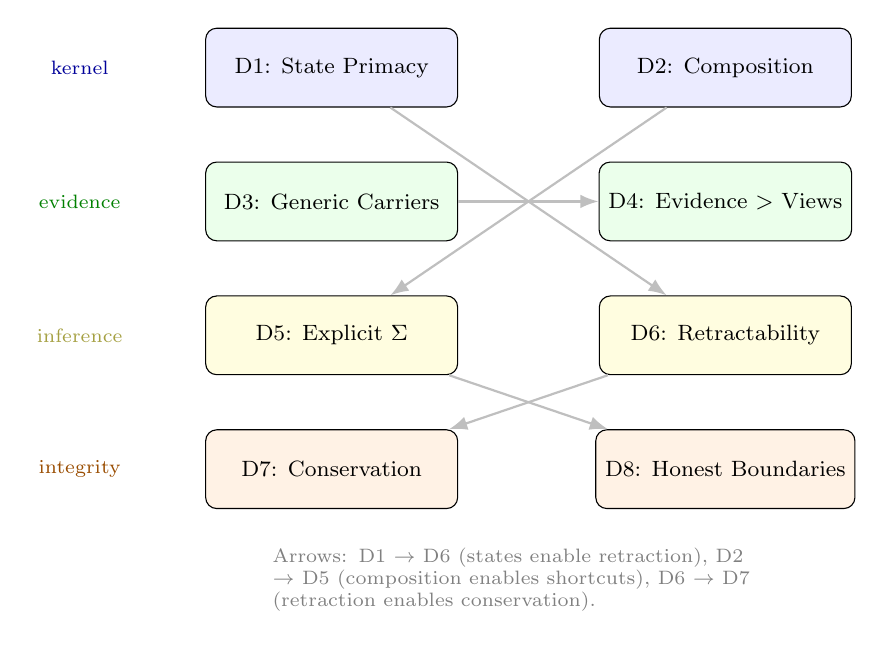
\begin{tikzpicture}[
  >=Latex,
  every node/.style={font=\footnotesize},
  dbox/.style={draw, rounded corners=4pt, minimum width=32mm,
              minimum height=10mm, align=center},
]
  % Kernel layer
  \node[dbox, fill=blue!8] (d1) at (0, 5) {D1: State Primacy};
  \node[dbox, fill=blue!8] (d2) at (5, 5) {D2: Composition};

  % Evidence layer
  \node[dbox, fill=green!8] (d3) at (0, 3.3) {D3: Generic Carriers};
  \node[dbox, fill=green!8] (d4) at (5, 3.3) {D4: Evidence $>$ Views};

  % Inference layer
  \node[dbox, fill=yellow!12] (d5) at (0, 1.6) {D5: Explicit $\Sigma$};
  \node[dbox, fill=yellow!12] (d6) at (5, 1.6) {D6: Retractability};

  % Meta layer
  \node[dbox, fill=orange!10] (d7) at (0, -0.1) {D7: Conservation};
  \node[dbox, fill=orange!10] (d8) at (5, -0.1) {D8: Honest Boundaries};

  % Layer labels (placed further left, vertically centered on each row)
  \node[font=\scriptsize, text=blue!60!black] at (-3.2, 5) {kernel};
  \node[font=\scriptsize, text=green!50!black] at (-3.2, 3.3) {evidence};
  \node[font=\scriptsize, text=yellow!60!black] at (-3.2, 1.6) {inference};
  \node[font=\scriptsize, text=orange!60!black] at (-3.2, -0.1) {integrity};

  % Dependency arrows
  \draw[->, thick, gray!50] (d1) -- (d6);
  \draw[->, thick, gray!50] (d2) -- (d5);
  \draw[->, thick, gray!50] (d3) -- (d4);
  \draw[->, thick, gray!50] (d6) -- (d7);
  \draw[->, thick, gray!50] (d5) -- (d8);

  % Annotation — placed well below the D7/D8 boxes
  \node[font=\scriptsize, text=gray, text width=65mm, align=left]
    at (2.5, -1.5) {Arrows: D1 $\to$ D6 (states enable retraction),
    D2 $\to$ D5 (composition enables shortcuts),
    D6 $\to$ D7 (retraction enables conservation).};
\end{tikzpicture}
\caption{The eight desiderata organized by layer.  Arrows show
enablement relationships: D1 (state primacy) enables D6
(retractability); D2 (compositional extraction) enables D5 (explicit
side conditions for compiled shortcuts); D6 (retractability) enables
D7 (conservation).}
\label{fig:desiderata-layers}
\end{figure}

\maplecourt{%
Maple Court's building model satisfies all eight desiderata.
It carries states (D1), combines sensor reports additively (D2),
handles binary, Dirichlet, and Normal-Gamma evidence (D3), derives
strength and confidence as views (D4), gates compiled chain rules on
BN screening-off (D5), retracts miscalibrated sensor data (D6),
conserves evidence under retraction (D7), and reports where local
chaining fails (D8).  The desiderata are not abstract stipulations
imposed from outside---they are the properties that make a building
automation system trustworthy.}


%% ═══════════════════════════════════════════════════════════════════
\part{The Calculus in Depth}
\label{part:calculus}
%% ═══════════════════════════════════════════════════════════════════

\chapter{The World-Model Calculus}
\label{ch:world-models}

What does it mean for a system to carry uncertain knowledge?  It means
the system has a \emph{state} that can be revised as new information
arrives, and that can be \emph{queried} to extract answers about the
world.  The world-model calculus makes this precise.

\section{The General Interface}

At its most abstract, a world model has three things: something it
knows (a \emph{state}), questions it can ask (\emph{queries}), and a
way to extract answers from what it knows.  In Lean, this is a
typeclass with three typed parameters and three operations:

\begin{lstlisting}[language={}]
class WorldModel (State Query V : Type*) where
  revise  : State -> State -> State
  empty   : State
  extract : State -> Query -> V
\end{lstlisting}

\noindent
A \code{State} is what the system carries.  A \code{Query} is what
the system may ask.  $V$ is the type in which extracted answers live.
\code{revise} combines two states.  \code{empty} is the state of
knowing nothing.  \code{extract} answers a query from a state.

No laws are assumed at this level.  How
$\mathrm{extract}(\mathrm{revise}(W_1, W_2), q)$
relates to the individual extractions depends on the \emph{revision
regime}---a choice that determines the character of the calculus.

The value type $V$ is generic.  Choosing $V$ determines the domain:

\medskip
\begin{center}
\begin{tabular}{ll}
\toprule
\textbf{Value type $V$} & \textbf{Domain} \\
\midrule
$(n^+, n^-)$ & Binary observations \\
$(\alpha_1,\ldots,\alpha_k)$ & Multi-valued observations \\
$(n, \textstyle\sum x_i, \sum x_i^2)$ & Continuous observations \\
$\mathbb{C}$ & Quantum amplitudes \\
\bottomrule
\end{tabular}
\end{center}
\medskip

\noindent
Each of these carries more information than a bare probability: the
sufficient statistics retain what is needed for further Bayesian
updating, not just a point estimate.  Classical probabilities are
always available as \emph{views}---lossy projections from richer
carriers (Chapter~\ref{ch:views}).%
\footnote{The first three carriers are fully formalized in Lean
(Chapter~\ref{ch:evidence}).  The amplitude carrier $\mathbb{C}$
connects to Meredith's framework~\cite{meredith2026ccc} and is a
natural future instance.}

\noindent
The query type is equally generic.  It may be a simple propositional
language, a first-order or higher-order logic, a temporal query
(Chapter~\ref{ch:temporal}), an intensional-sort query
(Chapter~\ref{ch:intensional}), or a deontic modality
(Chapter~\ref{ch:governance}).  Logical structure appears wherever
the query space carries it---quantified and higher-order queries are
instances of the generic \code{Query} parameter, not extensions to a
lower theory.

The generality of this interface is genuine.  Seven neighboring
frameworks---Markov Logic Networks, ProbLog, PLN v0.9,
classical FOL, the Giry monad, and the $\rho$-calculus---are
shown to be \code{WorldModel} instances with proved
extraction agreements; NARS has a proved Galois connection
to PLN evidence (Chapter~\ref{ch:bridges}).
Pearl's structural
causal models~\cite{Pearl2009} are also \code{WorldModel} instances: the
state is a system of structural equations $X_i = f_i(\mathrm{pa}(X_i),
U_i)$ plus a joint distribution over exogenous variables~$U_i$.
Revision updates the equations or incorporates observational data.
Queries span Pearl's three-level causal hierarchy: observational
($P(Y \mid X = x)$), interventional ($P(Y \mid \mathrm{do}(X = x))$),
and counterfactual.  The do-calculus rules become compiled rewrites
under causal-DAG side conditions---exactly the pattern developed in
Part~III.  Revision of SCMs with conflicting equations
is \emph{not} additive; it requires the overlap-aware or trust-gated
regimes described in the next section.%
\footnote{Formalized in
\codepath{Mettapedia/Logic/WorldModelBase.lean}.}

\maplecourt{%
Each Maple Court apartment carries a private state over questions
such as whether a pipe is leaking or whether the shower is running.
Querying ``Is there a pipe leak?'' extracts binary evidence
$(1, 4)$---one leak alarm and four no-alarm readings.  Shared spaces carry a building-level state over hallway
humidity and elevator health.  The same three operations---revise,
empty, extract---appear at both scales.}


\section{Revision Regimes}

Chapter~\ref{chap:overview} introduced four revision regimes.  Here
we develop the additive regime in depth and situate the others
concretely.

\begin{description}
\item[Additive.]  Independent updates compose by addition:
  $\mathrm{extract}(W_1 + W_2, q) = \mathrm{extract}(W_1, q) +
  \mathrm{extract}(W_2, q)$.  This is the main tractable regime and
  the subject of~\S\ref{sec:additive-regime}--\S\ref{sec:naturality}.

\item[Overlap-aware.]  When two sensor networks share a source---say,
  two apartments' humidity sensors both pick up the same hallway
  vent---naive addition double-counts.  An explicit overlap correction
  removes the shared component.

\item[Trust-gated.]  When a tenant's verbal report contradicts an
  automated sensor, the system must weigh source authority.  Revision
  is gated by trust scores: not symmetric, not additive.

\item[Coalition.]  When multiple apartments must agree before updating
  the building model---e.g., a majority vote on whether the elevator
  needs maintenance---only coalitions satisfying an actionability
  predicate may revise.
\end{description}

\noindent
The additive regime is developed in full generality in this book.
The others are formalized in Lean and treated here in less depth,
but they are \emph{not} future work---the key theorems are
proved, and this section presents them.


\section{The Non-Additive Perimeter}
\label{sec:non-additive}

The non-additive regimes are not afterthoughts.  They formalize
the situations where naive evidence addition fails: correlated
sources, trust-weighted merges, and quorum-based consensus.  The
Lean formalization contains $\sim$60 theorems across these
regimes, all kernel-checked with 0~sorry.

\subsection{The Overlap Extraction Law}

When two evidence sources share information, addition
double-counts the shared component.  The
\code{OverlapWorldModel} replaces the additive extraction law
with an overlap-corrected version:
\[
  \mathrm{extract}(\mathrm{revise}(W_1, W_2), q)
  = \mathrm{combine}\bigl(
      \mathrm{extract}(W_1, q),\;
      \mathrm{extract}(W_2, q),\;
      \mathrm{overlap}(W_1, W_2, q)
    \bigr).
\]
When the overlap function returns zero (independent sources),
this reduces to the additive law.  When overlap is nonzero, the
correction prevents double-counting.

\begin{theorem}[Additivity recovery under independence
  (\claimCore{})]
\label{thm:additive-of-independent}
If $\mathrm{overlap}(W_1, W_2, q)$ is trivial for all~$q$, then
the overlap extraction law reduces to the additive extraction
law: $\mathrm{extract}(\mathrm{revise}(W_1, W_2), q) =
\mathrm{extract}(W_1, q) + \mathrm{extract}(W_2, q)$.
\end{theorem}

\noindent
This theorem is the formal boundary between the additive and
overlap regimes: additivity is not assumed---it is
\emph{recovered} when the independence condition holds.%
\footnote{Formalized in
\codepath{Mettapedia/Logic/WorldModelOverlap.lean}
(7~theorems, 0~sorry).}

The \code{SubtractiveOverlapLayer} makes the correction explicit
via inclusion-exclusion:
\[
  \mathrm{extract}(\mathrm{merge}(W_1, W_2), q)
  = \mathrm{extract}(W_1, q) + \mathrm{extract}(W_2, q)
  - \mathrm{overlap}(W_1, W_2, q).
\]
When overlap is zero (independent sources), the subtraction
vanishes and additive extraction is recovered exactly
(\code{inclusionExclusion\_of\_zero\_overlap}).  This is the
formal analogue of the Dempster-Shafer subadditivity correction.

In the probability hypercube
(Knuth--Skilling~\cite{KnuthSkilling2012}), the overlap regime
corresponds to the Dempster-Shafer vertex (subadditive belief
functions), where $\mathrm{bel}(A \cup B) \ge
\mathrm{bel}(A) + \mathrm{bel}(B) - \mathrm{bel}(A \cap B)$:

\medskip
\begin{center}
\begin{tabular}{llll}
\toprule
\textbf{WM regime} & \textbf{Logic} & \textbf{Repr.} &
  \textbf{Hypercube vertex} \\
\midrule
Additive & Boolean & point &
  classical Bayesian \\
Overlap-aware & Boolean & bounds &
  imprecise probability \\
Evidence-tracking & Heyting & 2D bounds &
  PLN evidence \\
Trust-gated & Heyting & point &
  weighted trust \\
\bottomrule
\end{tabular}
\end{center}
\medskip

\noindent
Each regime is determined by two independent structural
decisions: does the event algebra satisfy excluded middle
(Boolean vs.\ Heyting), and does the representation track
per-channel evidence or summarize to a point?  The KS
representation theorem gives the unique algebra for each
vertex.%
\footnote{Classification kernel-checked in
\codepath{Mettapedia/Logic/WMHypercubeClassification.lean}
(17~items, 0~sorry).}

The carrier axis is orthogonal: binary, Dirichlet, and
Normal-Gamma carriers are all formalized and compose with any
merge-law vertex.  The quantum/classical boundary is whether the
carrier has a lattice ordering: $\mathbb{C}$ does not, placing
quantum inference at a distinct vertex
(\code{quantum\_not\_classical}).%
\footnote{Hypercube positions are kernel-checked in
\codepath{Mettapedia/ProbabilityTheory/KnuthSkilling/Examples/%
PreciseVsImpreciseGrounded.lean}
(1071~lines, 26~theorems, 0~sorry).}


\subsection{Coalition Revision and Semitopology}

The \code{CoalitionWorldModel} requires a proof of
$\mathrm{actionable}(W_1, W_2)$ before revision can fire.
The actionable sets form a \emph{semitopology}: a family closed
under union but \emph{not} under intersection---strictly weaker
than a topology.

\begin{example}[Quorum semitopology]
Three agents $\{0, 1, 2\}$.  Coalitions $\{0,1\}$ and $\{0,2\}$
are both actionable (two-agent quorum).  But their intersection
$\{0\}$ is \emph{not} actionable---a single agent cannot force
revision.  This is the formal content of ``a majority must agree.''
\end{example}

\begin{theorem}[Additivity recovery under semitopological
  independence (\claimCore{})]
\label{thm:additive-of-semitopo}
If both states' supports are actionable and disjoint, then the
coalition extraction law reduces to the additive extraction law.
\end{theorem}

\noindent
The deepest result connects overlap to coalitions:

\begin{theorem}[Additivity recovery after forgetting
  non-actionable overlap (\claimCore{})]
\label{thm:additive-recovery}
When the overlap footprint between two states is non-actionable
(the shared evidence does not form a legitimate coalition),
forgetting the overlap recovers additivity on the remainders.
\end{theorem}

\noindent
This is the formal answer to ``when can we safely treat
correlated sources as independent?''---when the correlation
structure is below the actionability threshold.%
\footnote{Formalized in
\codepath{Mettapedia/Logic/PLNSemitopology.lean}
(241~lines, 23~theorems) and
\codepath{Mettapedia/Logic/PLNSemitopologyProvenanceBridge.lean}
(294~lines, 22~theorems).  Both 0~sorry.}

\maplecourt{%
Two apartments share a hallway humidity vent.  Their sensor
readings are correlated---naive addition double-counts the shared
signal.  The overlap layer explicitly tracks this correlation.
When the building steward forgets the shared vent's contribution,
the remaining per-apartment evidence is independent, and
additivity recovers.  The quorum structure matters too: if the
building requires two apartments to agree before revising the
hallway humidity state, a single apartment's reading cannot force
an update---that is the semitopological actionability constraint.}%
\footnote{Both examples kernel-checked:
\codepath{Mettapedia/Logic/PLNMapleCourtOverlapDemo.lean}
(8~theorems) and
\codepath{Mettapedia/Logic/PLNMapleCourtCoalitionDemo.lean}
(13~theorems), both 0~sorry.}

\subsection{The Additive Regime as the Main Powerhouse}

The non-additive perimeter is formalized because it is
\emph{real}---correlated sensors exist, quorum requirements
exist, and the book would be dishonest to pretend otherwise.
But the additive regime remains the main powerhouse for two
reasons: (1)~it is where the profile-hom equivalence, BN
exactness, provenance tracking, and compiled inference all live,
and (2)~the recovery theorems above show that the additive
regime is \emph{approached} whenever overlap is small or
non-actionable.  The rest of this chapter develops the additive
regime in depth; the non-additive theorems appear again when
needed (multideduction overlap in
Chapter~\ref{ch:scale-control}; forgetting in
Chapter~\ref{ch:state-ops}).

To be explicit: the book's strongest exact theorems---profile-hom
equivalence, BN chain/fork/collider exactness, evidence
conservation, sleep consolidation---are additive-regime theorems.
The non-additive regimes are real and formalized ($\sim$90
theorems, 0~sorry), but they are not yet developed to comparable
breadth.  This asymmetry is not weakness; it is intellectual
hygiene about what has been proved and what remains open.


\section{The Additive Regime}
\label{sec:additive-regime}

The additive regime assumes that state revision is additive, that the
value carrier is an additive commutative monoid, and that extraction
commutes with addition:

\begin{lstlisting}[language={}]
class AdditiveWorldModel (State Query V : Type*)
    [AddCommMonoid State] [AddCommMonoid V]
    extends WorldModel State Query V where
  revise_eq_add : forall W1 W2, revise W1 W2 = W1 + W2
  empty_eq_zero : empty = 0
  extract_add   : forall W1 W2 q,
    extract (W1 + W2) q = extract W1 q + extract W2 q
  extract_zero  : forall q, extract 0 q = 0
\end{lstlisting}

\noindent
The decisive law is \code{extract\_add}.  It says that revising states
and then extracting is the same as extracting first and then combining
answers in the carrier~$V$.  Together with \code{extract\_zero}, this
makes the curried map
$W \mapsto (\lambda q.\; \mathrm{extract}(W, q))$ an additive monoid
homomorphism from states to answer profiles:
\[
  \widehat{\mathrm{extract}} \;:\;
  \code{State} \;\xrightarrow{\;+\;}\;
  (\code{Query} \to V)
\]
This one arrow is the entire semantic interface of the additive regime.
Everything else---views, compiled rules, inference control---is built
on top of it.

Extraction is additive for \emph{every} choice of $V$.  But downstream
projections (strength, confidence, Born rule $|\cdot|^2$) are
\emph{not} additive---they are lossy views.%
This asymmetry determines
the inference architecture and is developed in
Chapter~\ref{ch:views}.%
\footnote{Formalized in
\codepath{Mettapedia/Logic/PLNWorldModelGeneric.lean}
and \codepath{Mettapedia/Logic/WorldModelCore.lean}.}

For the implementer: to build a new additive world model, implement
\code{extract} and prove the two laws.  The rest of the stack---views,
compiled BN inference, forgetting, provenance---works automatically for
any conforming instance.

\begin{figure}[htbp]
\centering
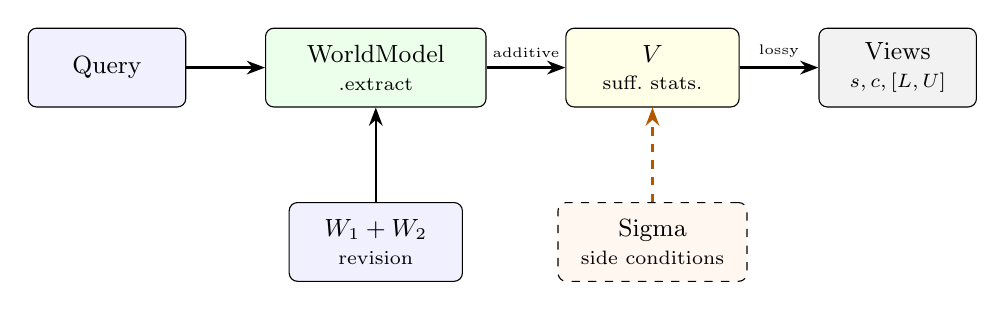
\begin{tikzpicture}[
  >=Stealth,
  every node/.style={font=\small},
  box/.style={draw, rounded corners=3pt, align=center,
              minimum height=10mm},
]
\node[box, fill=blue!6, minimum width=20mm] (q) {Query};
\node[box, fill=green!8, minimum width=28mm, right=10mm of q] (wm)
  {\code{WorldModel}\\[-1pt]{\scriptsize\code{.extract}}};
\node[box, fill=yellow!10, minimum width=22mm, right=10mm of wm] (ev)
  {$V$\\[-1pt]{\scriptsize suff.\ stats.}};
\node[box, fill=gray!10, minimum width=20mm, right=10mm of ev] (view)
  {Views\\[-1pt]{\scriptsize$s, c, [L,U]$}};

\draw[->, thick] (q) -- (wm);
\draw[->, thick] (wm) -- node[above, font=\tiny] {additive} (ev);
\draw[->, thick] (ev) -- node[above, font=\tiny] {lossy} (view);

\node[box, fill=blue!6, minimum width=22mm, below=12mm of wm] (rev)
  {$W_1 + W_2$\\[-1pt]{\scriptsize revision}};
\draw[->, thick] (rev) -- (wm);

\node[draw, dashed, rounded corners=3pt, fill=orange!6,
      minimum width=24mm, minimum height=10mm,
      below=12mm of ev, align=center] (sig)
  {\code{Sigma}\\[-1pt]{\scriptsize side conditions}};
\draw[->, dashed, thick, orange!70!black] (sig) -- (ev);
\end{tikzpicture}
\caption{The additive world-model interface.  A query is answered by
extracting a value from the state; views are lossy projections.
Revision ($+$) combines states.  Side conditions ($\Sigma$) enable
compiled rewrites.}
\label{fig:query-worldmodel-flow}
\end{figure}


\section{Side Conditions}

The kernel interface makes no structural assumptions: any additive
state that extracts values qualifies.  But most \emph{fast} inference
depends on structure.  When Maple Court's building model uses a
Bayesian network to compute humidity-leak correlations, it relies on
the DAG factorization and d-separation properties of that network.
When the deduction rule computes $P(C \mid A)$ from $P(B \mid A)$ and
$P(C \mid B)$, it relies on the \emph{screening-off} assumption:
\[
  P(C \mid A, B) = P(C \mid B).
\]
Once you know $B$, knowing $A$ provides no additional information
about $C$.  In a chain BN $A \to B \to C$, the DAG structure
guarantees this (d-separation).  In a general world model, it is an
explicit side condition that must be verified.

These structural assumptions make tractable inference \emph{exact}
rather than approximate.  Every compiled rewrite carries
its $\Sigma$ explicitly---there are no hidden assumptions.

For the implementer: when a compiled rule fires, it checks (or
requires proof of) its $\Sigma$.  If the side condition is not met,
the rule does not apply.


\section{Five Typed Rules of the Additive Regime}
\label{sec:algebraic-core}

The profile-hom equivalence has five immediate algebraic consequences.
They are not five independent axioms: all five \emph{derive} from the
single condition that extraction is a commutative-monoid homomorphism.
They are stated here algebraically;
Chapter~\ref{ch:typed}~\S\ref{sec:five-as-rewrites} develops their
concrete incarnation as pattern-matching rewrite rules.

\begin{enumerate}
\item \textbf{Extraction additivity} (\claimCore{}).%
  \footnote{Claim labels: \claimCore{} = unconditional algebraic fact;
  \claimConditional{} = holds under stated side conditions;
  \claimBoundary{} = impossibility / no-go result;
  \claimOperational{} = implementation-level property.
  These categories are used throughout the book.}
  \[\mathrm{extract}(\mathrm{revise}(W_1, W_2),\, q)
    = \mathrm{combine}(\mathrm{extract}(W_1, q),\;
                         \mathrm{extract}(W_2, q)).\]

\item \textbf{Zero extraction} (\claimCore{}).
  $\mathrm{extract}(0, q) = 0$.

\item \textbf{Revision commutativity} (\claimCore{}).
  $\mathrm{revise}(W_1, W_2) = \mathrm{revise}(W_2, W_1)$.

\item \textbf{Revision associativity} (\claimCore{}).
  $\mathrm{revise}(\mathrm{revise}(W_1, W_2), W_3)
  = \mathrm{revise}(W_1, \mathrm{revise}(W_2, W_3))$.

\item \textbf{Combine identity} (\claimCore{}).
  $\mathrm{combine}(e, 0) = e$.
\end{enumerate}

\begin{theorem}[\code{wmCore\_sound\_of\_addCommMonoidHom},
kernel-checked]
\label{thm:algebraic-core}
If an interpretation satisfies the homomorphism and zero conditions, all
five rule soundness conditions follow.  The world-model term algebra
modulo rewriting is the free commutative monoid; extraction is the
unique homomorphism to $(V, +, 0)$.
\end{theorem}

\noindent
These five rules organize into a $2 \times 2$ square along two
orthogonal axes:

\begin{center}
\begin{tabular}{lll}
\toprule
& \textbf{Plain} & \textbf{+ Congruence} \\
\midrule
\textbf{Raw (schematic)} & all rules fire & + context descent \\
\textbf{Guarded (faithful)} & side-condition oracle & + context descent \\
\bottomrule
\end{tabular}
\end{center}

\noindent
This is presented \emph{abstractly} here.
Chapter~\ref{ch:typed} incarnates the $2 \times 2$ square as
concrete typed rewrite rules over the 13-axis vertex family.


\section{The Sequent-Calculus Presentation}
\label{sec:sequent-calculus}

The additive regime has a natural sequent-calculus presentation.
Two contexts: an \emph{evidence context}~$\Gamma$ (a finite multiset
of state fragments) and a \emph{side-condition context}~$\Sigma$.
Four rules suffice:

\[
\frac{}{\Sigma; \varnothing \vdash_{\mathrm{wm}} 0} \;(\text{Unit})
\qquad
\frac{}{\Sigma; \{W\} \vdash_{\mathrm{wm}} W} \;(\text{Ev})
\]
\[
\frac{\Sigma; \Gamma \vdash_{\mathrm{wm}} W \quad
      \Sigma; \Delta \vdash_{\mathrm{wm}} W'}
     {\Sigma; \Gamma \uplus \Delta \vdash_{\mathrm{wm}} (W + W')}
\;(\text{Rev})
\qquad
\frac{\Sigma; \Gamma \vdash_{\mathrm{wm}} W}
     {\Sigma; \Gamma \vdash q \Downarrow \mathrm{extract}(W, q)}
\;(\text{Extract})
\]

\noindent
Evidence compositionality makes the query-revision rule admissible:
if $\Gamma \vdash q \Downarrow e$ and $\Delta \vdash q \Downarrow e'$,
then $\Gamma \uplus \Delta \vdash q \Downarrow (e + e')$.

Links are \emph{queries}, not connectives: $A \Rightarrow B$ is a
query $\mathrm{link}(A, B)$ against the revised world model, not an
object-level implication.


\section{The Evidence Proof System}
\label{sec:evidence-proof-system}

The four rules of \S\ref{sec:sequent-calculus} are not arbitrary.
Under the Curry-Howard correspondence---the identification of proofs
with programs and propositions with types---the evidence calculus is a
classical proof system.  The evidence state is the proof term, the
query is the proposition, and the four rules are the four structural
rules of sequent calculus.

\medskip
\begin{center}
\begin{tabular}{ll}
\toprule
\textbf{Proof Theory}   & \textbf{Evidence Algebra} \\
\midrule
Proof term (context)     & Evidence state $W$ \\
Proposition (judgment)   & Query $q$ \\
Cut rule                 & Revision ($W_1 + W_2$) \\
Evaluation               & Extraction ($\mathrm{extract}(W, q)$) \\
Weakening                & Forgetting \\
Exchange                 & Commutativity ($W_1 + W_2 = W_2 + W_1$) \\
Contraction              & Self-revision ($W + W$) \\
\bottomrule
\end{tabular}
\end{center}
\medskip

\noindent
Reading the table downward:

\begin{description}
\item[Cut.]  The Rev rule combines two evidence judgments into one.
  In proof theory, cut combines two sequent proofs by matching a
  conclusion with a hypothesis.  In the evidence calculus, cut
  matches exactly: the combined evidence for query~$q$ equals the
  sum of the parts, $\mathrm{extract}(W_1 + W_2, q) =
  \mathrm{extract}(W_1, q) + \mathrm{extract}(W_2, q)$.  This is
  \code{extract\_add}---the defining law of the additive regime.

\item[Weakening.]  Discarding a hypothesis without affecting the
  remaining conclusions.  In the evidence calculus, forgetting a
  source's contribution $W_{\mathrm{forget}}$ from a combined state
  $W_{\mathrm{keep}} + W_{\mathrm{forget}}$ leaves valid evidence
  for $W_{\mathrm{keep}}$ alone.  The evidence may decrease but does
  not become invalid.

\item[Exchange.]  Reordering hypotheses.  Addition in
  \code{AddCommMonoid} is commutative, so
  $W_1 + W_2 = W_2 + W_1$.  The order of evidence composition
  is irrelevant.

\item[Contraction.]  Using a hypothesis more than once.
  Self-revision $W + W$ doubles the evidence sample size
  ($\mathrm{ess}(W + W) = 2 \cdot \mathrm{ess}(W)$) without
  changing the strength ratio.  This is contraction: the same
  evidence source may be cited twice, yielding more certainty
  but the same posterior mean.
\end{description}

\begin{theorem}[Structural completeness (\claimCore{})]
\label{thm:structural-rules}
The additive evidence algebra over \code{BinEvNat} satisfies all four
structural rules of classical sequent calculus: cut, weakening,
exchange, and contraction.%
\footnote{Formalized in
\codepath{Mettapedia/Logic/EvidenceProofSystem.lean}
(10~theorems, 0~sorry).}
\end{theorem}

\noindent
The word \emph{classical} is precise.  An intuitionistic proof system
satisfies cut, weakening, and exchange, but not contraction: using a
hypothesis twice may change the proof.  The evidence algebra satisfies
all four.  This is because addition is idempotent in information
content (the posterior ratio $n^+ / (n^+ + n^-)$ is invariant under
$W \mapsto W + W$), even though the raw counts double.  A linear
proof system would drop weakening (every hypothesis must be used
exactly once); the evidence calculus allows forgetting, so it is not
linear.

\paragraph{A worked example.}
Let $e_1 = (3, 1)$ and $e_2 = (2, 2)$.

\smallskip
\begin{description}
\item[Cut:]  $e_1 + e_2 = (5, 3)$.  Total evidence
  $\mathrm{ess} = 8 = 4 + 4$.
\item[Weakening:]  Forget $e_2$: the remaining evidence
  $e_1 = (3, 1)$ is still valid, with $\mathrm{ess} = 4$.
\item[Exchange:]  $e_2 + e_1 = (5, 3) = e_1 + e_2$.
\item[Contraction:]  $e_1 + e_1 = (6, 2)$, with
  $\mathrm{ess} = 8 = 2 \times 4$.  The strength
  $6/8 = 3/4$ equals the original $3/4$.
\end{description}

\paragraph{What this means.}
The evidence calculus is not merely an algebraic bookkeeping system
with inference heuristics attached.  It is a proof system in the
technical sense: it has judgments (evidence for queries), structural
rules (the four above), and a cut-elimination direction (revision
increases total evidence, the normalization direction).  The
propositions-as-types reading is available to anyone who wants it:
the evidence state \emph{is} the proof, the query \emph{is} the
proposition, and the extraction \emph{is} the evaluation.


\section{Model, Calculus, and Soundness}
\label{sec:calculus-soundness}

Every formal system has two faces.  The \emph{model} says what
things mean: \code{AdditiveWorldModel} defines extraction
semantically.  The \emph{calculus} says what you can do: three
operational rules that manipulate evidence states.  The
\emph{soundness theorem} says these two faces agree.

\begin{figure}[htbp]
\centering
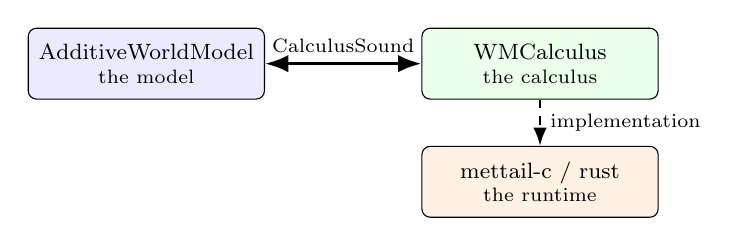
\begin{tikzpicture}[
  >=Latex, every node/.style={font=\footnotesize},
  box/.style={draw, rounded corners=3pt, minimum width=30mm,
              minimum height=9mm, align=center}
]
  \node[box, fill=blue!8] (model) at (0, 0)
    {\code{AdditiveWorldModel}\\[-1pt]\scriptsize the model};
  \node[box, fill=green!8] (calc) at (5, 0)
    {\code{WMCalculus}\\[-1pt]\scriptsize the calculus};
  \node[box, fill=orange!10] (impl) at (5, -1.5)
    {mettail-c / rust\\[-1pt]\scriptsize the runtime};

  \draw[<->, very thick] (model) -- node[above, font=\scriptsize]
    {\code{CalculusSound}} (calc);
  \draw[->, thick, dashed] (calc) -- node[right, font=\scriptsize]
    {implementation} (impl);
\end{tikzpicture}
\caption{Three layers, two boundaries.  The book proves the upper
  boundary (\code{CalculusSound}).  The lower boundary
  (implementation correctness) is the implementor's responsibility.}
\label{fig:model-calculus-soundness}
\end{figure}

The calculus is a structure with three fields:

\begin{lstlisting}[language={}]
structure WMCalculus (State Query Ev : Type*) where
  revise  : State -> State -> State       -- the cut rule
  extract : State -> Query -> Ev          -- the evaluation rule
  forget  : Option (State -> State -> State) -- the weakening rule
\end{lstlisting}

\noindent
An implementor provides three functions.  The soundness property
says they agree with the algebraic model:

\begin{lstlisting}[language={}]
structure CalculusSound (wmc : WMCalculus State Query Ev) where
  revise_correct  : forall W1 W2, wmc.revise W1 W2 = W1 + W2
  extract_correct : forall W q,   wmc.extract W q  = extract W q
\end{lstlisting}

\noindent
Two equalities.  The calculus's revision is the model's addition.
The calculus's extraction is the model's extraction.

\begin{theorem}[\code{CalculusSound} inheritance (\claimCore{})]
\label{thm:calculus-sound-inheritance}
If \code{wmc} satisfies \code{CalculusSound}, then:
\begin{enumerate}
\item \code{extract\_add} holds for the calculus (evidence
  revision is compositional).
\item Sequential composition works (multi-step revision is
  associative).
\item Zero preservation holds (empty state gives empty evidence).
\item All four structural rules (cut, weakening, exchange,
  contraction) transfer from the model to the calculus.
\end{enumerate}
The proof is four rewrites.%
\footnote{Formalized in
\codepath{Mettapedia/Logic/WMCalculusSoundness.lean}
(5~theorems, 0~sorry).}
\end{theorem}

\noindent
The mathematical tower---KS foundations, measure theory,
hypercube classification, 700+ theorems---does not need to be
re-proved.  It transfers by soundness.

\paragraph{A concrete example.}
Suppose mettail-rust implements \code{revise} as integer addition
on $(n^+, n^-)$ pairs and \code{extract} as field projection.
The implementor proves two equalities: addition agrees,
projection agrees.  From that proof, every theorem in this book
that mentions \code{extract\_add} becomes a theorem about the
Rust implementation.  The implementor never opens a Lean file
about measure theory or the KS representation.  Those results
arrive by soundness.

\paragraph{The philosophical point.}
There is one boundary between mathematics and engineering.
\code{CalculusSound} is that boundary.  On one side: the entire
algebraic and measure-theoretic development.  On the other side:
three functions in C or Rust.  Cross the boundary once, correctly,
and the entire mathematical tower transfers.  The proof of
\code{CalculusSound} is the smallest possible obligation with the
largest possible payoff.

\paragraph{GSLT connection.}
In Meredith's GSLT framework, the calculus is the rewrite system
and the model is the denotational semantics.
\code{CalculusSound} is the standard soundness theorem: rewrites
agree with denotations.

\paragraph{Decentralized agents.}
If two agents both prove \code{CalculusSound} for their (possibly
different) implementations, their evidence composes---not by
policy, but by theorem.  Trust becomes a mathematical property.


\section{The Profile-Hom Equivalence}
\label{sec:profile-hom}

The additive interface has a clean universal property.

\begin{theorem}[Profile-hom equivalence (\claimCore{})]
\label{thm:universal-property}
An additive world model is exactly an additive monoid homomorphism
from states to answer profiles:
\[
  \code{AdditiveWorldModel}(\code{State}, \code{Query}, V)
  \;\simeq\;
  \mathrm{AddMonoidHom}(\code{State},\; \code{Query} \to V)
\]
Both directions are definitional: the world-model interface IS the
additive morphism, and vice versa, up to definitional equality in
Lean---no propositional reasoning is needed.%
\footnote{Formalized in \codepath{Mettapedia/Logic/WorldModelCore.lean}.
The structural equivalence \code{equivGSLTProfileHom} has both
roundtrips by \code{rfl}.}
\end{theorem}

\paragraph{The terminal extensional world model.}
The answer-profile object $\mathrm{Prof}(\code{Query}, V) :=
\code{Query} \to V$ is itself an additive world model: extraction is
function evaluation, so both laws hold by \code{rfl}.  Every additive
world model maps into it via extraction, and the map is unique up to
the profile it determines.  This makes $\mathrm{Prof}(\code{Query}, V)$
the \emph{terminal} extensional world model.

In categorical terms, additive world models over \code{Query} form a
slice category $\mathbf{AddCommMon} / \mathrm{Prof}(\code{Query}, V)$,
and $\mathrm{Prof}(\code{Query}, V)$ is its terminal object.  A
morphism between additive world models is a commuting triangle:

\begin{lstlisting}[language={}]
structure WorldModelHom (State1 State2 Query V) where
  hom  : State1 ->+ State2
  comm : forall W q, extract (hom W) q = extract W q
\end{lstlisting}

\noindent
The canonical morphism to the terminal model \emph{is}
extraction.\footnote{Open program: is this slice category enriched
in a useful way?}

\paragraph{Why this matters.}
The universal property means that the \emph{entire} additive
world-model interface is one algebraic condition.  The five rules
are not independent axioms---they all derive from the single
requirement that extraction is an \code{AddMonoidHom}.  This does
not trivialize the project: the hard work is in choosing expressive
state spaces, proving no-go theorems, and certifying fast inference
paths.  But it makes the \emph{interface} minimal and the
\emph{achievements} sharper.

For the implementer: you can swap state representations without
changing the semantics.  Any two additive world models producing the
same answer profiles are extensionally equivalent.

For the general \code{WorldModel} without additivity laws, no
analogous universal property is known.  This is one reason the additive
regime is the main exact specialization: it is the regime where the
categorical picture is sharpest.


\section{Naturality Across Signatures}
\label{sec:naturality}

When the query language changes---by adding atoms, extending the
signature, or translating between formalisms---the extraction map
must \emph{commute} with the translation.  For a signature morphism
$\sigma : \mathrm{Sig}_1 \to \mathrm{Sig}_2$:
\[
  \mathrm{extract} \circ \mathrm{reindex}_\sigma
  \;=\;
  \mathrm{reindex}_\sigma \circ \mathrm{extract}
\]
This is the \emph{satisfaction condition} of an institution: truth
(here: evidence extraction) is invariant under change of
notation.%
\footnote{Formalized as
\code{satisfactionCondition\_is\_naturality} in
\codepath{Mettapedia/Logic/PLNWorldModelInstitution.lean}.}
\footnote{Open program: the GSLT universal theorem---every
graph-structured lambda theory with parallel composition naturally
induces a WorldModel.  See Meredith~\cite{meredith2026ccc}.}


\section{The Solomonoff--De Finetti Foundation}

The previous sections built the algebraic and categorical interface.
This section addresses the foundational question: \emph{why} is
revision-as-addition the right choice?  The answer comes from
exchangeability theory.

The \nuPLN{} framework of Nil Geisweiller~\cite{nuPLN2026} grounds the
calculus in Solomonoff Universal Induction.  The global probability
space $(\Omega, \mathcal{F}, \nu)$ corresponds to a world-model state
where $\Omega$ is the set of possible worlds.  The universal
distribution~$\nu$ defines a prior over generators; Bayesian updating
with observed evidence produces the posterior.

The crucial insight is that de~Finetti's representation
theorem~\cite{definetti1937} justifies evidence counts as
\emph{sufficient statistics}.  For exchangeable binary sequences, the
counts $(n^+, n^-)$ contain all the information needed for Bayesian
updating.  Under a Beta prior, the posterior is
$\text{Beta}(\alpha + n^+, \beta + n^-)$.

For the implementer: evidence counts are not an arbitrary design
choice.  De~Finetti says they are the mathematically forced
representation for exchangeable data.

\paragraph{Giry monad and Markov kernels.}
The categorical underpinning is the Giry monad: the functor sending
a measurable space to its space of probability measures.  The
formalization proves that Kyburg's flattening \emph{is} the Giry bind,
with all three monad laws.  The complete justification chain:
\[
  \text{exchangeability}
  \;\to\; \text{de Finetti mixture}
  \;\to\; \text{Kyburg flattening}
  \;\to\; \text{Giry bind}
  \;\to\; \text{evidence sufficiency}
\]
Each arrow is proved.  Together they show that revision-as-addition
is not an arbitrary choice but a categorical necessity under
exchangeability.%
\footnote{See
\codepath{Mettapedia/ProbabilityTheory/GiryMonad.lean}
and
\codepath{Mettapedia/ProbabilityTheory/DeFinettiConnection.lean}
}%
\footnote{Open program: the terminal
\code{WorldModel (Measure $\Omega$) Query} instance remains future
work.}


\section{Four Verbs: Revise, Query, Forget, Explain}

The world-model interface supports four operations:

\begin{description}
\item[\textbf{Revise}] (kernel): combine two states ($W_1 + W_2$ in
  the additive regime; general merge otherwise).

\item[\textbf{Query}] (kernel): extract a value from a state for a
  given question.

\item[\textbf{Forget}] (state management): remove evidence under
  explicit scope constraints, preserving answers outside the scope
  (Chapter~\ref{ch:state-ops}).

\item[\textbf{Explain}] (state management): trace which observations
  support an answer, via provenance-enriched evidence
  (Chapter~\ref{ch:state-ops}).
\end{description}

\noindent
Revision and querying are the minimal interface; forgetting and
explaining show \emph{why} the kernel stores states rather than bare
values.  A bare value can be queried but cannot be partially retracted
or audited.

The $2 \times 2$ calculus square of~\S\ref{sec:algebraic-core} is
the abstract face of a full natively typed presentation: the five
algebraic rules encode as typed rewrite rules over a 13-axis vertex
family, developed in Chapter~\ref{ch:typed}.  Native types do not
introduce a second semantics---they expose, at the rewrite level, the
structural behavior already present in the semantic kernel.


\section{A Worked Instance: Dirichlet over Worlds}

For finite propositional scope (atoms indexed by $\mathrm{Fin}(n)$),
the additive world model can be instantiated concretely.  The state is
a \emph{world table}:
\[
  \mathrm{JointEvidence}(n) := \mathrm{Fin}(2^n) \to
  \mathbb{R}_{\ge 0}^{\infty}
\]
interpreted as Dirichlet pseudo-counts over the $2^n$ possible worlds.
Each coordinate records how much evidence supports that world.
Extraction sums counts over worlds compatible with each query:
for $\mathrm{prop}(A)$, sum where $A$ is true vs.\ false; for
$\mathrm{link}(A, B)$, sum where $A \wedge B$ vs.\ $A \wedge \neg B$.
Revision is pointwise addition of pseudo-counts.%
\footnote{Formalized in
\codepath{Mettapedia/Logic/PLNJointEvidence.lean}.}

This instance satisfies all the laws of
\code{AdditiveWorldModel}: extraction commutes with revision, and the
empty world table (all zeros) extracts zero for every query.  It is
the \emph{most informative} additive world model for finite
propositional scope --- every other model is a projection of it.
The no-go theorem (Chapter~\ref{ch:no-go}) shows that this
projection is genuinely lossy: per-link projections cannot
reconstruct the joint.

%% ─────────────────────────────────────────────────────────────────

\chapter{Evidence Carriers and Revision}
\label{ch:evidence}

What kind of object does extraction return?  The previous chapter left
$V$ generic.  This chapter makes it concrete: $V$ is a family of
\emph{sufficient-statistic carriers}, each storing what is needed for
further Bayesian updating in a particular domain.  The algebraic
discipline---revision as addition, information ordering as componentwise
comparison---is the same for every carrier.  Only the domain changes.

\section{The Generic Evidence Pattern}

Every carrier in the additive regime satisfies two generic laws:

\begin{enumerate}
\item \textbf{Revision is addition.}  Combining two bodies of evidence
  is commutative, associative, with a zero (no evidence).
  Algebraically: $V$ is an \code{AddCommMonoid}.
\item \textbf{Information is ordered.}  A partial order where ``more
  data'' means ``at least as informative.''
\end{enumerate}

\noindent
Two additional algebraic structures enrich the carrier family:
a \emph{quantale tensor} for composing evidence along inference
chains, and a \emph{Heyting algebra} (complete lattice with Frame
structure) supporting intuitionistic implication and complement.
These were originally developed for binary evidence
(\S\ref{sec:binary-tensor}--\S\ref{sec:binary-heyting}) and have
now been extended to the full $k$-ary Dirichlet family:
coordinatewise multiplication gives a commutative monoid tensor,
and the pointwise lattice gives a complete Heyting algebra for
all~$k$.%
\footnote{Formalized in
\codepath{Mettapedia/Logic/EvidenceDirichletQuantale.lean}
(13~theorems, 0~sorry).  Normal-Gamma carriers have a
formalized information partial order
(\codepath{Mettapedia/Logic/EvidenceNormalGammaLattice.lean},
10~theorems, 0~sorry) but intentionally no quantale tensor ---
sufficient statistics for unknown mean and variance are not
counts.}

Every exponential family with sufficient statistics instantiates this
pattern:

\begin{center}
\begin{tabular}{ll}
\toprule
\textbf{Domain} & \textbf{Sufficient statistics} \\
\midrule
Binary       & $(n^+, n^-)$ \\
$k$-valued   & $(\alpha_1, \ldots, \alpha_k)$ \\
Continuous   & $(n, \sum x_i, \sum x_i^2)$ \\
Count data   & $(n, \sum x_i)$ \\
Covariance   & $(n, \sum x_i x_i^\top)$ \\
\bottomrule
\end{tabular}
\end{center}

\noindent
The first three are formalized in this book
(cf.\ the carrier table in Chapter~\ref{ch:world-models}).  The rest
are natural future instances requiring only new \code{AddCommMonoid}
implementations---no changes to the calculus itself.


\section{The Three Formalized Carriers}

\paragraph{Binary (Beta-Binomial).}
The simplest carrier handles yes/no queries.
$\mathsf{BinaryEvidence} := (n^+, n^-) \in
\mathbb{R}_{\ge 0}^\infty \times \mathbb{R}_{\ge 0}^\infty$,
where $n^+$ counts positive and $n^-$ counts negative observations.
Under a Beta prior $\text{Beta}(\alpha, \beta)$, the posterior is
$\text{Beta}(\alpha + n^+, \beta + n^-)$.  The Laplace-smoothed
strength is $s = (1 + n^+) / (2 + n)$.%
\footnote{Formalized in \codepath{Mettapedia/Logic/BinaryEvidence.lean}
and \codepath{Mettapedia/Logic/EvidenceBeta.lean}.}

\paragraph{Dirichlet-Multinomial ($k$-valued).}
For queries with $k$ outcomes---``Is the elevator normal, slow, or
faulty?''---evidence is a count vector
$(\alpha_1, \ldots, \alpha_k) \in \mathbb{R}_{\ge 0}^k$.
The posterior mean for category~$i$ is
$\alpha_i / \sum_j \alpha_j$; confidence is
$(\sum \alpha_j) / (\sum \alpha_j + k)$.%
\footnote{Formalized in \codepath{Mettapedia/Logic/EvidenceDirichlet.lean}.}

\paragraph{Normal-Gamma (continuous).}
For real-valued observations such as humidity readings, the sufficient
statistics are $(n, \sum x_i, \sum x_i^2)$.  The prior is
$\text{Normal-Gamma}(\mu_0, \kappa_0, \alpha_0, \beta_0)$; the
posterior parameters update as
$\kappa_n = \kappa_0 + n$,
$\mu_n = (\kappa_0 \mu_0 + \sum x_i) / \kappa_n$,
$\alpha_n = \alpha_0 + n/2$.%
\footnote{Formalized in \codepath{Mettapedia/Logic/EvidenceNormalGamma.lean}.}

\medskip\noindent
In each case, revision is componentwise addition of sufficient
statistics.  The algebra does not change across carriers; only the
domain does.

\begin{theorem}[Sleep consolidation (\claimCore{})]
\label{thm:sleep-consolidation}
For each of the three primary carriers:
$\mathrm{posterior}(\pi, e_1 \hplus e_2)
= \mathrm{posterior}(\mathrm{posterior}(\pi, e_1), e_2)$.
Batch replay of deferred observations yields the same posterior as
sequential updating.  This guarantee is exercised on real data in
Chapter~\ref{ch:carrier-validation}: gas sensor drift
(\S\ref{sec:gas-drift}), Kalman temporal filtering, and GJP
forecast aggregation (\S\ref{sec:gjp-forecasting}).
\end{theorem}

\maplecourt{%
Maple Court instantiates all three: Beta for leak, occupancy, and
shower sensors; Normal-Gamma for humidity readings; Dirichlet for the
three-valued \emph{LaundryState} and \emph{ElevatorHealth}.
Querying elevator health with counts $(40, 8, 2)$ yields posterior
means $(0.80, 0.16, 0.04)$ with confidence~$0.83$.  Revising with
10~more ``normal'' observations shifts to $(50, 8, 2)$ and confidence
$0.86$.  Sleep consolidation means the apartment can buffer overnight
readings and batch-update at dawn with identical results.}%
\footnote{The Maple Court example enjoys three-way conformance:
(1)~30 PeTTa runtime tests across four \code{.metta} files, all
passing; (2)~34 algebraic theorems in
\codepath{Mettapedia/Logic/PLNMapleCourtDemo.lean}; and
(3)~4 unconditional kernel-checked conformance theorems via a
specialized reflection checker (the Ramsey36 pattern: write a
simple pattern match the kernel can reduce, then close with
\code{decide}).  See
\codepath{Mettapedia/Conformance/MapleCourtWMConformance.lean}.}


\section{Revision as Addition}

Why is revision componentwise addition?  The foundational justification
via de~Finetti's exchangeability theorem was given in
Chapter~\ref{ch:world-models}, \S``The Solomonoff--De Finetti
Foundation.''  Here we show the concrete mechanics: adding counts
corresponds to Bayesian conjugate updating:
\[
  \text{Beta}(\alpha + n_1^+, \beta + n_1^-)
  \;\;\xrightarrow{+\;(n_2^+, n_2^-)}\;\;
  \text{Beta}(\alpha + n_1^+ + n_2^+, \beta + n_1^- + n_2^-)
\]
Revision is addition because it is the algebraic shadow of conjugate
updating.  The same pattern extends to all three primary carriers:
\begin{align*}
  \text{Dirichlet:}\quad
  &(\alpha_1, \ldots, \alpha_k) \hplus (\beta_1, \ldots, \beta_k)
  = (\alpha_1 + \beta_1, \ldots, \alpha_k + \beta_k) \\
  \text{Normal-Gamma:}\quad
  &(n_1, s_1, q_1) \hplus (n_2, s_2, q_2)
  = (n_1 + n_2,\; s_1 + s_2,\; q_1 + q_2)
\end{align*}
In every case, revision is componentwise addition of the sufficient
statistics.  The algebra does not change; only the domain does.


\section{Information Ordering}

Evidence values are partially ordered by information content.  For
binary evidence:
\[
  (n_1^+, n_1^-) \le (n_2^+, n_2^-) \iff
  n_1^+ \le n_2^+ \;\wedge\; n_1^- \le n_2^-
\]
This extends componentwise to Dirichlet vectors and Normal-Gamma
statistics.  The ordering makes each carrier a lattice (meet $=$
componentwise min, join $=$ componentwise max).

For the Normal-Gamma carrier, the information order has additional
structure: zero (the empty-evidence state) is bottom, and
aggregation is monotone---adding evidence never decreases
information.  Unlike the counting carriers (binary, Dirichlet),
the Normal-Gamma carrier does not admit a quantale tensor:
sufficient statistics for unknown mean and variance are not
counts, and coordinatewise multiplication does not preserve the
conjugate structure.  This asymmetry is by design---the
information order and additive revision are the generic
properties; the tensor is carrier-specific.%
\footnote{Formalized in
\codepath{Mettapedia/Logic/EvidenceNormalGammaLattice.lean}
(10~theorems, 0~sorry).}

The key property: this is a \emph{partial} order.  $(3, 0)$ and
$(0, 3)$ are incomparable---they contain the same total but differ in
kind.  No single scalar captures ``how much evidence'' there is.

\begin{figure}[htbp]
\centering
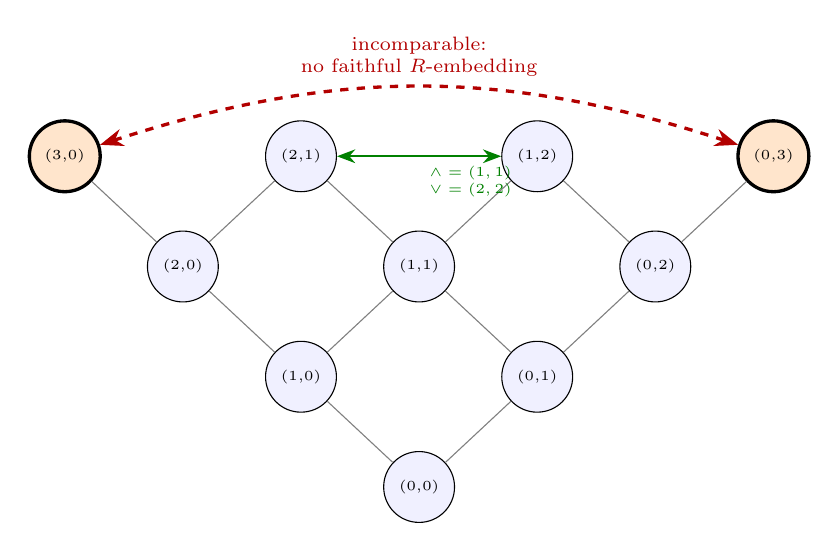
\begin{tikzpicture}[
  >=Stealth,
  every node/.style={font=\scriptsize},
  ev/.style={draw, circle, minimum size=9mm, inner sep=1pt, fill=blue!6},
  inc/.style={draw, circle, minimum size=9mm, inner sep=1pt, fill=orange!20,
              very thick},
]
\node[ev] (00) at (3, 0) {$\scriptscriptstyle(0,0)$};
\node[ev] (10) at (1.5, 1.4) {$\scriptscriptstyle(1,0)$};
\node[ev] (01) at (4.5, 1.4) {$\scriptscriptstyle(0,1)$};
\node[ev] (20) at (0, 2.8) {$\scriptscriptstyle(2,0)$};
\node[ev] (11) at (3, 2.8) {$\scriptscriptstyle(1,1)$};
\node[ev] (02) at (6, 2.8) {$\scriptscriptstyle(0,2)$};
\node[inc] (30) at (-1.5, 4.2) {$\scriptscriptstyle(3,0)$};
\node[ev] (21) at (1.5, 4.2) {$\scriptscriptstyle(2,1)$};
\node[ev] (12) at (4.5, 4.2) {$\scriptscriptstyle(1,2)$};
\node[inc] (03) at (7.5, 4.2) {$\scriptscriptstyle(0,3)$};
\draw[thin, gray] (00) -- (10); \draw[thin, gray] (00) -- (01);
\draw[thin, gray] (10) -- (20); \draw[thin, gray] (10) -- (11);
\draw[thin, gray] (01) -- (11); \draw[thin, gray] (01) -- (02);
\draw[thin, gray] (20) -- (30); \draw[thin, gray] (20) -- (21);
\draw[thin, gray] (11) -- (21); \draw[thin, gray] (11) -- (12);
\draw[thin, gray] (02) -- (12); \draw[thin, gray] (02) -- (03);
\draw[<->, very thick, red!70!black, dashed]
  (30) to[bend left=18]
  node[above, font=\scriptsize, text width=32mm, align=center]
    {incomparable:\\no faithful $\mathbb{R}$-embedding}
  (03);
\draw[<->, thick, green!50!black] (21) --
  node[below right, font=\tiny, text width=22mm, align=left]
    {$\wedge = (1,1)$\\$\vee = (2,2)$}
  (12);
\end{tikzpicture}
\caption{Hasse diagram of the binary evidence lattice.  Orange nodes
$(3,0)$ and $(0,3)$ are incomparable (the ``totality gate'').}
\label{fig:evidence-lattice}
\end{figure}


\section{Compositional Tensor for Binary Evidence}
\label{sec:binary-tensor}

When you know $A \Rightarrow B$ with evidence $e_{AB}$ and
$B \Rightarrow C$ with evidence $e_{BC}$, what can you say about
$A \Rightarrow C$?  For binary evidence, the quantale tensor
$\htensor$ composes evidence along inference chains:
\[
  (a^+, a^-) \htensor (b^+, b^-) =
  (a^+ \cdot b^+,\; a^+ \cdot b^- + a^- \cdot b^+)
\]
with unit $(1, 0)$.  This is a complete lattice with $\htensor$
distributing over arbitrary joins (a quantale).

\begin{theorem}[Quantale transitivity (\claimCore{})]
\label{thm:quantale-trans}
$e_{AB} \htensor e_{BC} \le e_{AC}$ in the information ordering.
Equality holds under screening-off.%
\footnote{Formalized in
\codepath{Mettapedia/Logic/EvidenceQuantale.lean}.}
\end{theorem}

\noindent
The tensor gives a sound lower bound for chained inference.  Exact
equality requires the screening-off side condition
(Chapter~\ref{ch:bn-models}).%
\footnote{Open program: a generic quantale for Dirichlet or
Normal-Gamma evidence would require defining a compositional tensor
on count vectors.}


\section{Logical Operations for Binary Evidence}
\label{sec:binary-heyting}

Binary evidence forms a Heyting algebra:

\begin{definition}[Heyting implication (\claimCore{})]
\[
  (a^+, a^-) \Rightarrow (b^+, b^-) =
  \Big(\,\begin{cases} \top & \text{if } a^+ \le b^+ \\
                        b^+ & \text{otherwise}\end{cases},\;\;
        \begin{cases} \top & \text{if } a^- \le b^- \\
                        b^- & \text{otherwise}\end{cases}\,\Big)
\]
satisfying $a \le (b \Rightarrow c) \iff a \wedge b \le c$.
\end{definition}

\noindent
Excluded middle fails: $a \vee \neg a \ne \top$, because absence of
evidence is not evidence of absence.  The ``totality gate'':
$(3,0)$ and $(0,3)$ are incomparable, so no faithful
$\mathbb{R}$-embedding exists.%
\footnote{Formalized in
\codepath{Mettapedia/Logic/HeytingValuationOnEvidence.lean}.}%
\footnote{The Heyting structure has been extended to $k$-ary
Dirichlet evidence: \codepath{Mettapedia/Logic/EvidenceDirichletQuantale.lean}
(13~theorems, 0~sorry).  The Boolean-to-Heyting categorical bridge is in
\codepath{Mettapedia/Logic/BooleanHeytingBridge.lean} (4~theorems).}


\section{Theoretical Foundations}

Four deeper connections ground the evidence algebra.

\paragraph{The De Finetti bridge.}
For an infinite exchangeable binary sequence, de~Finetti's
representation theorem~\cite{definetti1937} asserts the existence of a
latent parameter~$\theta$ such that, given~$\theta$, the observations
are i.i.d.\ Bernoulli($\theta$).  The joint distribution is a mixture:
\[
  P(X_1 = x_1, \ldots, X_n = x_n)
  = \int_0^1 \theta^{n^+}(1 - \theta)^{n^-} \, d\mu(\theta)
\]
where $n^+ = \sum x_i$ and $n^- = n - n^+$.  The pair $(n^+, n^-)$
is the sufficient statistic of this mixture: no other function of
the data adds information about $\theta$.  This is why revision is
addition: adding counts IS the algebraically forced update under
exchangeability.  The proof extends to Dirichlet-Multinomial and
Normal-Gamma via the same mixture logic.%
\footnote{Formalized in
\codepath{Mettapedia/ProbabilityTheory/DeFinettiConnection.lean}
}

\paragraph{Walley predictive intervals.}
The Imprecise Dirichlet Model~\cite{Walley1996BagOfMarbles} gives
prior-free interval bounds on predictive probabilities.  Where
Bayesian credible intervals depend on the choice of prior, Walley's
intervals are robust at the cost of wider bounds.  The calculus
supports both: the carrier stores the counts, and the interval
semantics is a choice of view (Chapter~\ref{ch:views}).

\paragraph{Knuth--Skilling foundations.}
Knuth and Skilling~\cite{KnuthSkilling2012} derive probability as
the unique consistent valuation on a lattice of propositions,
generalizing Cox's theorem to distributive lattices.  At the
world-model layer, probabilities arise as valuations on Boolean
subsets of worlds (the Kolmogorov story).  At the evidence layer, the
rules weaken from Boolean equalities to Heyting inequalities.  The
bridge enables factor-graph variable elimination over
Knuth--Skilling-valued factors.%
\footnote{Formalized in
\codepath{Mettapedia/ProbabilityTheory/KnuthSkilling/}.}

\paragraph{The bivariate structure.}
The world-model calculus has \emph{state-side} additivity:
$\mathrm{extract}(W_1 + W_2, q) = \mathrm{extract}(W_1, q) +
\mathrm{extract}(W_2, q)$.  Knuth--Skilling adds \emph{obs-side}
additivity: for disjoint queries $q_1, q_2$,
$\mathrm{extract}(W, q_1 \vee q_2) =
\mathrm{extract}(W, q_1) + \mathrm{extract}(W, q_2)$
(where $\vee$ is the join in a lattice of queries).
These are two laws on different arguments of the same bivariate
extractor.  A unification with laws on both arguments---a
\emph{stateful valuation}---is one of the most promising open
directions (see also \S\ref{sec:gslt-open-program}).%
\footnote{Open program: a \code{StatefulValuation} typeclass with
both state-side and obs-side laws.  The probability
hypercube~\cite{StayWells2026} classifies theories by which
combination of these laws they satisfy.}

\paragraph{The KS-Evidence-Measure triangle.}
The evidence carriers, the KS representation theorem, and the
measure-valued terminal world model form a commuting triangle:
\begin{center}
\begin{tabular}{@{}c@{}}
KS ordered semigroup $\xrightarrow{\;\Theta = \mathrm{total}\;}$
$(\mathbb{R}_{\ge 0}^\infty, +)$
$\xrightarrow{\;\bullet\,\mathrm{dirac}\;}$
\code{Measure}
\end{tabular}
\end{center}
The evidence carriers (binary, Dirichlet) satisfy the KS axioms
(ordered, associative, monotone).  The representation theorem
maps them into $\mathbb{R}_{\ge 0}^\infty$ via the total-evidence
function.  The measure bridge
(\code{evidenceToMeasure}) composes this with Dirac
weighting to produce a formal measure.  Additivity holds at
every vertex: $\hplus$ on evidence, $+$ on reals, $+$ on
measures.  The triangle says the WM evidence algebra is not an
ad-hoc design---it is the \emph{unique} algebra satisfying the
KS axioms, and the measure theory follows inevitably.%
\footnote{The KS formalization spans 126K~lines with 1,923
theorems (0~sorry for the core representation; 11~sorry in
experimental Shore-Johnson extensions).
The triangle bridge is in
\codepath{Mettapedia/Logic/KSEvidenceMeasureBridge.lean}.
The $\sigma$-additivity boundary
(\codepath{Mettapedia/ProbabilityTheory/KnuthSkilling/%
Counterexamples/SigmaAdditivityNecessity.lean})
proves that finitely additive measures do not automatically
extend to $\sigma$-additive ones---Step~C of the measure frontier
requires Scott continuity, which is a separate axiom.}


\section{What Evidence Algebra Is Not}

Evidence algebra is \emph{not} the complete probabilistic semantics.
It is a compositional bookkeeping layer.  The world-model state
carries strictly more information than the extracted per-query evidence
values.  The no-go theorem (Chapter~\ref{ch:no-go}) makes this
precise: per-link evidence cannot reconstruct the joint state.

Evidence tells you the score.  It does not tell you the game.
The correlations, the causal structure, the joint distribution over
worlds---those live in the state, not in the per-query counts.  This
is why the calculus stores states and extracts evidence, rather than
storing evidence directly.

\paragraph{Raw data vs.\ sufficient statistics.}
A system may also store the raw observations themselves---a
\emph{data-backed state}---and compress to sufficient statistics
on demand.  The compositionality theorem
\code{compress\_append} proves that compression is a monoid
homomorphism: compressing two raw-data batches separately and
adding the results gives the same sufficient statistics as
compressing the concatenated batch.%
\footnote{Formalized in
\codepath{Mettapedia/Logic/EvidentialLedger.lean}.}
This means the system can keep raw data for model switching or
distributional queries while using compressed statistics for
efficient $O(1)$ revision---the two representations are provably
compatible.

\paragraph{Evidence algebra is not quantale algebra.}
The binary evidence carrier forms a quantale (a complete lattice
with an associative tensor), but the PLN operations on that
carrier are \emph{not} the quantale operations.  Two concrete
divergences are kernel-checked:
\begin{enumerate}
\item \textbf{Revision $\neq$ supremum.}  Evidence revision
  ($\hplus$) adds counts: $(2,1) \hplus (1,2) = (3,3)$.  The
  lattice supremum takes componentwise max: $(2,1) \sqcup (1,2) =
  (2,2)$.  These are different---revision is conjugate update,
  supremum is information combination.
\item \textbf{Tensor strength $\neq$ strength product.}  The
  quantale tensor $(3,1) \otimes (2,2) = (6,2)$ has strength
  $6/8 = 0.75$.  The product of strengths is $0.75 \times 0.5 =
  0.375$.  Tensor on evidence does not distribute over the
  strength view.
\end{enumerate}
The positive characterization: when one evidence state dominates
the other componentwise, the supremum equals the dominating
state.  The quantale provides the algebraic skeleton; PLN fills
in the probabilistic flesh.%
\footnote{Formalized in
\codepath{Mettapedia/Logic/PLNQuantaleDivergence.lean}
(3~theorems, 0~sorry).}

%% ─────────────────────────────────────────────────────────────────

\chapter{State Operations}
\label{ch:state-ops}

If the world model were just a truth value, there would be nothing to
retract, nothing to audit, nothing to explain.  A number has no parts.
But a state has structure: it records which observations contributed to
which queries, and that structure supports operations that bare values
cannot.

This chapter develops the third and fourth verbs of the calculus:
\emph{forget} (partially retract evidence under scope constraints) and
\emph{explain} (trace which observations support an answer).

\section{Why Forgetting Matters}

A sensor reading from last Tuesday should eventually expire.  A privacy
constraint says apartment-level data must not persist in the building
model beyond 24~hours.  A correction says ``the batch of observations
from sensor~3 was miscalibrated; retract them.''  All of these are
forgetting operations.

Forgetting is not deletion.  It is a \emph{scoped retraction}: remove
evidence within a declared scope while provably preserving everything
outside it.  This requires the state to carry enough structure to
distinguish what came from where---which is precisely what provenance
provides.

\section{The Forgetting Layer}
\label{sec:forgetting}

A forgetting layer over a world model has four components:

\begin{lstlisting}[language={}]
structure ForgettingLayer (State Scope Query V)
    [WorldModel State Query V] where
  inScope    : Scope -> Query -> Prop
  forget     : Scope -> State -> State
  idempotent : forall S W, forget S (forget S W) = forget S W
  outsideInvariant :
    forall S W q, not (inScope S q) ->
      WorldModel.extract (forget S W) q = WorldModel.extract W q
\end{lstlisting}

\noindent
The key law is \code{outsideInvariant}: forgetting scope~$S$ preserves
the extracted value for every query outside~$S$.  In the answer-profile
language: forgetting changes the profile only within the declared scope.
Idempotence says forgetting the same scope twice is the same as
forgetting it once.%
\footnote{Formalized in
\codepath{Mettapedia/Logic/GenericWorldModelForgetting.lean}
.}

\maplecourt{%
The apartment forgets stale humidity readings after 6~hours: the scope
is ``humidity observations older than $t - 6\mathrm{h}$.''  Outside
that scope---motion detections, leak alarms---the profile is unchanged.
The building forgets laundry observations after 24~hours.  Each
layer's forgetting is independent and scope-delimited.}


\section{Conservation Theorems}
\label{sec:conservation}

Under \emph{exact inverse forgetting}---where forgetting scope~$S$
exactly undoes a revision~$\Delta$ that was entirely within~$S$---a
family of conservation laws holds.

\begin{theorem}[Evidence conservation (\claimCore{})]
\label{thm:conservation}
If $\Delta$ is a revision whose evidence lies entirely within scope~$S$
(i.e., $\forall W,\; \mathrm{forget}(S, W + \Delta) = W$), then for
every query~$q$ outside~$S$:
\begin{enumerate}
\item \textbf{Anti-hallucination}: $\mathrm{extract}(\Delta, q) = 0$.
  The revision contributes zero evidence outside its scope.
\item \textbf{Noether conservation}:
  $\mathrm{extract}(W + \Delta, q) = \mathrm{extract}(W, q)$.
  The revised state agrees with the base state outside the scope.
\item \textbf{Zero leakage}: the observation count of~$\Delta$ at~$q$
  is zero.
\end{enumerate}
\end{theorem}

\begin{theorem}[Exact-inverse no-go (\claimBoundary{})]
If a revision~$\Delta$ has nonzero evidence at any query outside
scope~$S$, then no forgetting operation can exactly undo~$\Delta$.
\end{theorem}

\noindent
This is the precise boundary: forgetting cannot undo what leaked.
The conservation theorems and the no-go are packaged as a single
\code{EvidenceConservationPack}.%
\footnote{Formalized in
\codepath{Mettapedia/Logic/PLNWorldModelConservationPack.lean}
.}

These results are the \emph{state-level, scoped-forgetting} face of
a broader family of evidence-conservation principles.
Goertzel~\cite{GoertzelEvidenceConservation2026} develops the
complementary \emph{inference-path} face: a discrete quantale Noether
theorem showing that reinforcement is constant along geodesic
inference paths, a hallucination bound showing that conclusion
strength is bounded by initial evidence mass, and an evidence
monotonicity theorem (a quantale data-processing inequality).
Together, the two perspectives establish that evidence can be neither
fabricated nor overcounted---whether the viewpoint is scoped
retraction of states or sequential chaining of inference steps.%
\footnote{The conservation principle extends beyond the commutative
setting.  Goertzel~\cite{GoertzelQMEvidence2026} argues that
evidence conservation under non-commutativity forces the evidence
lattice to be a Hilbert-space lattice, recovering the mathematical
structure of quantum mechanics from epistemological first principles.
This connects to the non-commutative vertex of the probability
hypercube (Chapter~\ref{ch:future}).}

\paragraph{Forgetting in the non-additive perimeter.}
The conservation and exact-inverse theorems above assume additive
revision.  In the overlap regime
(\S\ref{sec:non-additive}), exact forgetting requires stronger
conditions: the \code{SupportTrackedForgettingLayer} proves that
exact inverse is possible \emph{only} when the revision evidence
vanishes outside the forgotten scope.  The semitopology bridge
provides the recovery theorem
(Theorem~\ref{thm:additive-recovery}): when the overlap footprint
is non-actionable, forgetting the overlap recovers additivity on
the remainder---and the conservation laws apply to the
remainder.%
\footnote{Formalized in
\codepath{Mettapedia/Logic/GenericWorldModelForgetting.lean}
(193~lines, 6~theorems) and
\codepath{Mettapedia/Logic/PLNWorldModelSupportForgetting.lean}
(75~lines, 3~theorems).  Both 0~sorry.}


\section{Provenance and Explanation}
\label{sec:provenance}

Evidence tells you \emph{how much} support a query has.  Provenance
tells you \emph{where that support came from}.

\[
  \code{State}
  \;\xrightarrow{\;\text{extract-with-prov}\;}
  (\code{Query} \to \text{Ev-with-Prov})
  \;\xrightarrow{\;\text{erase prov.}\;}
  (\code{Query} \to V)
\]

\noindent
The first arrow produces evidence tagged with source identifiers
(which sensor, which batch, which time window).  The second erases
the tags, recovering ordinary evidence.  The composition equals
ordinary extraction---provenance is a refinement, not a replacement.
This is the same pattern as type erasure in programming languages or
audit trails in accounting: the enriched representation supports
richer operations (here, targeted forgetting), and the surface
representation is recovered by forgetting the enrichment.

The concrete realization is \code{TrackedWhichState}: a state that
carries, for each query, a multiset of provenance chunks.  Each chunk
records a source label and an evidence contribution.  The total
evidence is the sum over chunks; the provenance is the set of source
labels.%
\footnote{Formalized in
\codepath{Mettapedia/Logic/PLNProvenanceTrackedState.lean}
.}%
\footnote{The underlying provenance-semiring
framework~\cite{GreenKarvounarakisTannen2007} supports different
semiring choices for different provenance granularities.  The
\code{Which} semiring tracks which observations contributed; a
\code{KRelation} valued in \code{Which} is itself an
\code{AdditiveWorldModel} instance (the bridge is proved).  A
polynomial semiring would additionally track full derivation trees.
An end-to-end example exercising the LP provenance operator
\code{T\_P\_K\_LP\_seeded} through WM extraction and forgetting
appears in \S\ref{sec:derivation-tracking-demo}.}

Provenance is not metadata.  It is part of the structure of stateful
reasoning.  Without it, forgetting cannot be targeted: you would have
to discard everything or nothing.  With it, retraction is surgical.

\maplecourt{%
The building's hallway-humidity evidence carries provenance.
Sensor~A reports 3~readings above the threshold (morning); sensor~B
reports 2~below (afternoon).  The combined evidence is
$(3, 0) \hplus (0, 2) = (3, 2)$, with strength $3/5 = 0.6$ and
provenance $\{\mathrm{A}, \mathrm{B}\}$.  When sensor~A is found
to be miscalibrated, the steward forgets scope $\{\mathrm{A}\}$:
the evidence drops to $(0, 2)$ (sensor~B alone), strength falls to
$0/2 = 0$ (no positive readings remain), and provenance narrows to
$\{\mathrm{B}\}$.  Sensor~B's contribution is provably conserved.}

\begin{figure}[htbp]
\centering
\begin{tikzpicture}[
  >=Stealth, every node/.style={font=\small},
  src/.style={draw, rounded corners=2pt, minimum width=22mm,
              minimum height=8mm, align=center},
  ev/.style={draw, rounded corners=2pt, minimum width=28mm,
             minimum height=8mm, align=center, fill=yellow!10},
]
\node[src, fill=blue!10] (A) at (0, 0) {Sensor A\\{\scriptsize $(3, 0)$}};
\node[src, fill=green!10] (B) at (4, 0) {Sensor B\\{\scriptsize $(0, 2)$}};
\node[ev] (combined) at (2, -1.8)
  {Combined: $(3, 2)$\\{\scriptsize $s = 0.6$, prov = \{A, B\}}};
\draw[->, thick] (A) -- (combined);
\draw[->, thick] (B) -- (combined);

\node[font=\Large] at (6.5, -0.9) {$\xrightarrow{\text{forget A}}$};

\node[src, fill=gray!20, dashed] (A2) at (9, 0)
  {Sensor A\\{\scriptsize retracted}};
\node[src, fill=green!10] (B2) at (13, 0) {Sensor B\\{\scriptsize $(0, 2)$}};
\node[ev] (after) at (11, -1.8)
  {Remaining: $(0, 2)$\\{\scriptsize $s = 0$, prov = \{B\}}};
\draw[->, gray!40, dashed] (A2) -- (after);
\draw[->, thick] (B2) -- (after);
\end{tikzpicture}
\caption{Provenance-tracked forgetting in Maple Court.  Sensor~A's
contribution $(3, 0)$ is retracted; sensor~B's $(0, 2)$ is conserved.}
\label{fig:maple-court-provenance}
\end{figure}


\section{PLN Evidence Stamps as Provenance}
\label{sec:pln-stamps}

PLN v0.9\footnote{PLN v0.9: \texttt{github.com/trueagi-io/PLN},
tag \texttt{v0.9}.  430~lines of MeTTa implementing forward chaining
with stamp-based evidence tracking.} tracks provenance via
\emph{stamps}: each sentence carries a sorted list of observation IDs,
and before combining two sentences, the engine checks
\texttt{StampDisjoint}---whether their stamps share any IDs.  If they
do, the revision is blocked to prevent double-counting.

This is exactly the formal provenance discipline.  The correspondence:

\medskip
\begin{center}
\begin{tabular}{@{}ll@{}}
\toprule
\textbf{PLN v0.9} & \textbf{WM calculus} \\
\midrule
\texttt{StampDisjoint} & \code{Finset.Disjoint} on scope supports \\
\texttt{StampConcat} & \code{Finset.union} \\
Forget a source & \code{forgetScopedByScope} \\
\bottomrule
\end{tabular}
\end{center}
\medskip

\noindent
PLN v0.9 checks stamps at runtime; the WM calculus proves disjointness
at compile time via \code{decide}.  PLN v0.9 has no forgetting; the WM
calculus adds it with proved conservation.%
\footnote{Formalized in
\codepath{Mettapedia/Logic/PLNProvenanceInference.lean} (general
theory) and
\codepath{Mettapedia/Logic/PLNClassicExamples.lean}
(20~conformance checks).}

\subsection{Stepped Walkthrough: DeductionRevision with Provenance}

We step through the PLN v0.9 DeductionRevision example in full detail.

\paragraph{Step 1: The knowledge base.}
Four observations, encoded as a PeTTa atomspace:

\begin{lstlisting}[language={}]
def drKB : PeTTaSpace where
  facts := [inh "A" "B",   -- obs 0
            inh "A" "C",   -- obs 1
            inh "B" "D",   -- obs 2
            inh "C" "D"]   -- obs 3
  rules := []
\end{lstlisting}

\begin{figure}[htbp]
\centering
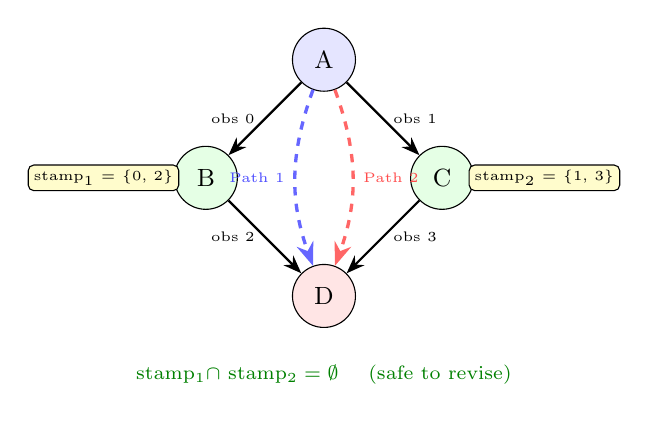
\begin{tikzpicture}[
  >=Stealth, every node/.style={font=\small},
  obs/.style={draw, circle, minimum size=8mm, inner sep=1pt},
  link/.style={->, thick},
  stamp/.style={font=\tiny, fill=yellow!20, draw, rounded corners=2pt,
                inner sep=2pt},
]
\node[obs, fill=blue!10] (A) at (0, 0) {A};
\node[obs, fill=green!10] (B) at (-1.5, -1.5) {B};
\node[obs, fill=green!10] (C) at (1.5, -1.5) {C};
\node[obs, fill=red!10] (D) at (0, -3) {D};
\draw[link] (A) -- node[left, font=\tiny] {obs 0} (B);
\draw[link] (A) -- node[right, font=\tiny] {obs 1} (C);
\draw[link] (B) -- node[left, font=\tiny] {obs 2} (D);
\draw[link] (C) -- node[right, font=\tiny] {obs 3} (D);
\draw[->, very thick, blue!60, dashed, bend right=20]
  (A) to node[left, font=\tiny, text=blue!70] {Path 1} (D);
\draw[->, very thick, red!60, dashed, bend left=20]
  (A) to node[right, font=\tiny, text=red!70] {Path 2} (D);
\node[stamp] at (-2.8, -1.5) {stamp$_1$ = \{0, 2\}};
\node[stamp] at (2.8, -1.5) {stamp$_2$ = \{1, 3\}};
\node[font=\scriptsize, text=green!50!black] at (0, -4)
  {stamp$_1 \cap$ stamp$_2 = \emptyset$ \quad (safe to revise)};
\end{tikzpicture}
\caption{DeductionRevision: two paths with disjoint provenance.}
\label{fig:deduction-revision-stamps}
\end{figure}

\paragraph{Step 2: Stamp disjointness (kernel-checked).}

\begin{lstlisting}[language={}]
def dr_stamp1 : Finset (Fin 4) := {0, 2}  -- Path 1: A->B->D
def dr_stamp2 : Finset (Fin 4) := {1, 3}  -- Path 2: A->C->D

theorem dr_stamps_disjoint :
    Disjoint dr_stamp1 dr_stamp2 := by decide

theorem dr_stamps_union :
    Finset.union dr_stamp1 dr_stamp2 = {0, 1, 2, 3} := by decide
\end{lstlisting}

\noindent
The \code{decide} tactic delegates to the kernel: Lean verifies
set-disjointness at type-checking time.  This is the compile-time
version of PLN v0.9's runtime \texttt{StampDisjoint}.

\paragraph{Step 3: Forgetting with conservation.}

\begin{lstlisting}[language={}]
-- Forgetting obs 0 does NOT affect Path 2
theorem dr_obs0_disjoint_path2 :
    Disjoint {0} dr_stamp2 := by decide

-- Path 1 retains only obs 2
theorem dr_path1_after_forget :
    dr_stamp1 \ {0} = {2} := by decide
\end{lstlisting}

\noindent
Forgetting observation~0 (A$\to$B) removes it from Path~1's stamp but
\emph{provably} leaves Path~2 intact.  This is a concrete instance of
the conservation theorem: evidence outside the forgotten scope is
preserved.

\begin{figure}[htbp]
\centering
\begin{tikzpicture}[
  >=Stealth, every node/.style={font=\small},
  obs/.style={draw, circle, minimum size=8mm, inner sep=1pt},
  link/.style={->, thick},
  stamp/.style={font=\tiny, fill=yellow!20, draw, rounded corners=2pt,
                inner sep=2pt},
  forgotten/.style={draw, circle, minimum size=8mm, inner sep=1pt,
                    fill=gray!20, dashed},
]
\node[font=\footnotesize\bfseries] at (-3.5, 0.5) {Before:};
\node[obs, fill=blue!10] (A1) at (-3.5, -0.5) {\tiny A};
\node[obs, fill=green!10] (B1) at (-4.5, -1.5) {\tiny B};
\node[obs, fill=green!10] (C1) at (-2.5, -1.5) {\tiny C};
\node[obs, fill=red!10] (D1) at (-3.5, -2.5) {\tiny D};
\draw[link, blue!60] (A1) -- (B1);
\draw[link, blue!60] (B1) -- (D1);
\draw[link, red!60] (A1) -- (C1);
\draw[link, red!60] (C1) -- (D1);
\node[stamp] at (-5.3, -2.5) {\{0,1,2,3\}};

\node[font=\Large] at (0, -1.5)
  {$\xrightarrow{\text{forget obs 0}}$};

\node[font=\footnotesize\bfseries] at (3.5, 0.5) {After:};
\node[obs, fill=blue!10] (A2) at (3.5, -0.5) {\tiny A};
\node[forgotten] (B2) at (2.5, -1.5) {\tiny B};
\node[obs, fill=green!10] (C2) at (4.5, -1.5) {\tiny C};
\node[obs, fill=red!10] (D2) at (3.5, -2.5) {\tiny D};
\draw[link, gray!40, dashed] (A2) -- (B2);
\draw[link, gray!40, dashed] (B2) -- (D2);
\draw[link, red!60] (A2) -- (C2);
\draw[link, red!60] (C2) -- (D2);
\node[stamp] at (5.3, -2.5) {\{1,2,3\}};
\node[font=\tiny, red!70!black] at (2.0, -0.8) {retracted};
\node[font=\tiny, green!50!black] at (5.0, -1.5) {conserved};
\end{tikzpicture}
\caption{Forgetting obs~0 (A$\to$B).  Path~1 loses its first link;
Path~2 is provably unaffected.  Stamp: $\{0,1,2,3\} \to \{1,2,3\}$.}
\label{fig:deduction-revision-forget}
\end{figure}


\subsection{Worked Example: Derivation Tracking with LP Provenance}
\label{sec:derivation-tracking-demo}

The DeductionRevision walkthrough above tracks provenance at the
stamp level---which observation IDs were consumed.  We now show a
deeper integration: provenance that flows through \emph{logic-program
rules}, is carried by a semiring-valued K-relation, participates in
WM extraction, and supports scoped forgetting with proved
conservation.  Every equation below is kernel-checked (28~theorems,
0~sorry).%
\footnote{Full source:
\codepath{Mettapedia/Logic/WMDerivationTrackingDemo.lean}.}

\paragraph{The scenario.}
Apartment~3B has two independent sensors: a pipe-leak detector
(observation~$o_1$) and a shower-running detector ($o_2$).  Three
LP rules propagate evidence through the building's causal model:

\begin{lstlisting}[language={}]
def mapleCourtProg : Program mapleCourtSig :=
  [rulePipeLeakToWallHumidity,       -- WallHumidity   <- PipeLeak
   ruleShowerToBathroomHumidity,     -- BathroomHumid. <- ShowerRunning
   ruleWallToMoldRisk]               -- MoldRisk       <- WallHumidity
\end{lstlisting}

\begin{figure}[htbp]
\centering
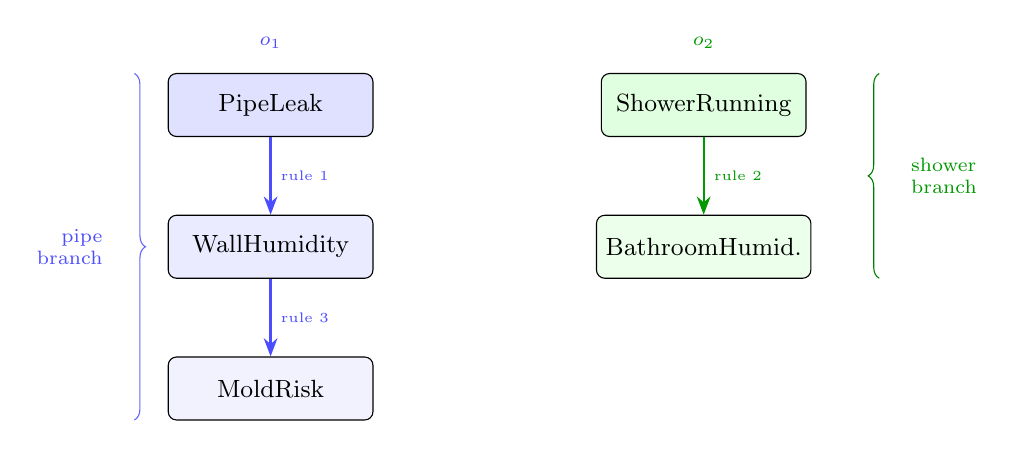
\begin{tikzpicture}[
  >=Stealth, every node/.style={font=\small},
  fact/.style={draw, rounded corners=3pt, minimum width=26mm,
               minimum height=8mm, align=center},
  rule/.style={->, thick},
]
\node[fact, fill=blue!12] (pipe) at (0, 0) {PipeLeak};
\node[fact, fill=green!12] (shower) at (5.5, 0) {ShowerRunning};
\node[fact, fill=blue!8] (wall) at (0, -1.8) {WallHumidity};
\node[fact, fill=green!8] (bath) at (5.5, -1.8) {BathroomHumid.};
\node[fact, fill=blue!5] (mold) at (0, -3.6) {MoldRisk};

\draw[rule, blue!70] (pipe) -- node[right, font=\tiny] {rule 1} (wall);
\draw[rule, green!60!black] (shower) -- node[right, font=\tiny] {rule 2} (bath);
\draw[rule, blue!70] (wall) -- node[right, font=\tiny] {rule 3} (mold);

\node[font=\scriptsize\bfseries, blue!70, anchor=south] at (0, 0.6) {$o_1$};
\node[font=\scriptsize\bfseries, green!60!black, anchor=south] at (5.5, 0.6) {$o_2$};

% Annotations
\draw[decorate, decoration={brace, amplitude=4pt, raise=2pt},
      blue!60] (-1.8, 0.4) -- (-1.8, -4) node[midway, left=6pt,
      font=\scriptsize, blue!70, align=right] {pipe\\branch};
\draw[decorate, decoration={brace, amplitude=4pt, raise=2pt, mirror},
      green!50!black] (7.8, 0.4) -- (7.8, -2.2) node[midway,
      right=6pt, font=\scriptsize, green!60!black, align=left]
      {shower\\branch};
\end{tikzpicture}
\caption{Maple Court derivation graph.  Observation $o_1$ feeds the
pipe branch (blue); observation $o_2$ feeds the shower branch
(green).  The two branches share no observations.}
\label{fig:derivation-tracking-dag}
\end{figure}

\paragraph{Seeded provenance.}
Observations enter as labeled seeds in the \code{Which}~semiring,
which tracks \emph{which} observations contributed to each derived
fact.  The seed for the pipe observation maps
$\mathrm{PipeLeak}$ to $\{o_1\}$ and everything else to~$\varnothing$:

\begin{lstlisting}[language={}]
def pipeSeed : KRelation mapleCourtSig (Which (Fin 2)) :=
  seedOf pipeLeak(*$_1$*) srcPipe    -- pipeLeak(*$_1$*) |-> {(*$o_1$*)}, else |-> (*$\varnothing$*)
\end{lstlisting}

\noindent
The seeded provenance operator \code{T\_P\_K\_LP\_seeded}
propagates labels through rules.  For wall humidity:

\begin{lstlisting}[language={}]
theorem T_P_K_LP_seeded_wallHumidity (seed I) :
  T_P_K_LP_seeded ... seed I wallHumidity(*$_1$*) =
    seed wallHumidity(*$_1$*) + I pipeLeak(*$_1$*)
\end{lstlisting}

\noindent
Read this as: the wall-humidity evidence at iteration~$I$ is
whatever was seeded directly, \emph{plus} whatever pipe-leak
evidence was available at the previous iteration---propagated
through rule~1.  The labels are carried by the semiring product;
no explicit label-passing code is needed.

\paragraph{Two-round closure.}
Two applications of \code{T\_P\_K\_LP\_seeded} suffice for the
longest derivation chain (PipeLeak $\to$ WallHumidity $\to$
MoldRisk).  The key results:

\begin{lstlisting}[language={}]
theorem pipeClosure_moldRisk :
  pipeClosure moldRisk(*$_1$*) = pipeProv            -- {(*$o_1$*)}
theorem pipeClosure_bathroomHumidity_zero :
  pipeClosure bathroomHumidity(*$_1$*) = 0           -- (*$\varnothing$*)
theorem showerClosure_bathroomHumidity :
  showerClosure bathroomHumidity(*$_1$*) = showerProv  -- {(*$o_2$*)}
theorem showerClosure_moldRisk_zero :
  showerClosure moldRisk(*$_1$*) = 0                 -- (*$\varnothing$*)
\end{lstlisting}

\noindent
The pipe observation $o_1$ flows through WallHumidity to MoldRisk
but \emph{not} to BathroomHumidity.  The shower observation $o_2$
flows to BathroomHumidity but \emph{not} to MoldRisk.  The
\code{Which} semiring tracks this automatically: no
branch-awareness is coded by hand.

\paragraph{WM extraction.}
The combined state
$\code{fullState} = \code{pipeClosure} + \code{showerClosure}$
is a \code{KRelation} valued in \code{Which}---and therefore an
\code{AdditiveWorldModel} instance.  Extraction is function
application:

\begin{lstlisting}[language={}]
theorem extract_fullState_moldRisk :
  AdditiveWorldModel.extract fullState moldRisk(*$_1$*)
    = pipeProv                                     -- {(*$o_1$*)}
theorem extract_fullState_bathroomHumidity :
  AdditiveWorldModel.extract fullState bathroomHumidity(*$_1$*)
    = showerProv                                   -- {(*$o_2$*)}
\end{lstlisting}

\noindent
The provenance labels survive extraction: the WM interface does not
erase them.  This is the key design point---provenance is part of
the evidence algebra, not a separate metadata channel.

\paragraph{Scoped forgetting with conservation.}
If the pipe sensor is later found to be miscalibrated, the
steward forgets scope $\{o_1\}$:

\begin{lstlisting}[language={}]
theorem forget_pipe_scope_moldRisk_zero :
  scopedTrackedEvidence
    (forgetScopedByScope scopePipe scopedFull) moldRisk(*$_1$*) = 0
theorem forget_pipe_scope_bathroomHumidity :
  scopedTrackedEvidence
    (forgetScopedByScope scopePipe scopedFull) bathroomHumidity(*$_1$*)
    = showerProv                                   -- {(*$o_2$*)}
\end{lstlisting}

\noindent
MoldRisk drops to zero---its only source was the pipe sensor.
BathroomHumidity is provably conserved---it came entirely from the
shower sensor, which is outside the forgotten scope.

The conservation theorem closes the loop:

\begin{lstlisting}[language={}]
theorem forget_after_remember_pipe_is_id :
  forgetScopedByScope scopePipe
    (scopedRemember sPipe pipeClosure scopedShower)
    = scopedShower
\end{lstlisting}

\noindent
Forgetting the pipe scope after re-remembering it returns exactly
the shower-only state: $\mathrm{forget} \circ \mathrm{remember}
= \mathrm{id}$ on the complement scope.  This is the Noether-style
conservation law from \S\ref{sec:conservation}, instantiated end-to-end
on a concrete LP derivation.%
\footnote{The symmetric case (forgetting the shower scope,
conserving the pipe branch) is also proved:
\code{forget\_shower\_scope} and
\code{forget\_after\_remember\_shower\_is\_id} in the same file.}

\maplecourt{%
This example exercises the full provenance pipeline:
labeled observation $\to$ LP rule propagation $\to$ semiring-valued
closure $\to$ WM extraction $\to$ scoped forgetting $\to$
conservation.  Every step is kernel-checked.  The building steward
can retract the pipe sensor's contribution to the world model and
know---not hope, but \emph{prove}---that the shower sensor's
contribution survives intact.  This is what D6 (Retractability)
and D1 (State Primacy) buy you when they are taken seriously.}


\subsection{Case Study: Evidence-Driven Ontology Repair}
\label{sec:pain-evidence-wm}

The derivation tracking demo above tracks sensor evidence through
LP rules.  We now apply the same evidence algebra to a different
domain: ontology engineering.  The task is to decide how to
reclassify a concept in a large ontology, using evidence from
multiple authoritative sources, with kernel-checked ranking and
sensitivity analysis.%
\footnote{Generic framework:
\codepath{Mettapedia/Logic/EvidentialLedger.lean}.
Concrete case:
\codepath{Mettapedia/Languages/GF/SUMO/PainEvidenceWM.lean}.
All 10~theorems by \code{decide}, 0~sorry.}

\paragraph{The problem.}
SUMO (Suggested Upper Merged Ontology) classifies Pain as a
\code{PathologicProcess}---a biological event on the Physical
branch.  But the axiom \code{(contraryAttribute Pleasure Pain)}
demands both arguments to be \code{Attribute} instances, which
live on the Abstract branch.  This is a type error.  Four
reclassification candidates exist: (a)~PathologicProcess (status
quo), (b)~EmotionalState, (c)~StateOfMind, (d)~split into
PainSensation + PainProcess.

\paragraph{The evidence ledger.}
Seven authoritative sources each contribute a support vector over
all four candidates simultaneously:

\begin{lstlisting}[language={}]
structure SourceItem (Source Candidate : Type*) where
  source  : Source
  kind    : EvidenceKind       -- empirical | textInterpreted | expertElicited
  support : Candidate (*$\to$*) BinEvNat  -- vector over ALL candidates
  note    : String
\end{lstlisting}

\noindent
Each source says something about \emph{every} candidate---not
just the one it favors.  The IASP definition, for instance, gives
$(0, 3)$ against PathologicProcess (strong refutation), $(1, 2)$
against EmotionalState (misses the sensory component), $(3, 0)$
for StateOfMind (direct match), and $(2, 0)$ for the split option.

\paragraph{Aggregation.}
The \code{aggregate} function folds support vectors by candidate
via componentwise addition---the same $\hplus$ revision that
drives the entire WM calculus:

\begin{lstlisting}[language={}]
theorem pathologic_total :
  aggregate painEvidence .pathologicProcess = (*$\langle$*)2, 16(*$\rangle$*)  -- refuted
theorem stateofmind_total :
  aggregate painEvidence .stateOfMind       = (*$\langle$*)12, 1(*$\rangle$*)  -- winner
theorem emotional_total :
  aggregate painEvidence .emotionalState    = (*$\langle$*)10, 3(*$\rangle$*)  -- runner-up
theorem split_total :
  aggregate painEvidence .split             = (*$\langle$*)6, 4(*$\rangle$*)   -- viable
\end{lstlisting}

\noindent
PathologicProcess is refuted ($2$ for vs.\ $16$ against).
StateOfMind leads EmotionalState ($12{:}1$ vs.\ $10{:}3$).
All totals are kernel-checked by \code{decide}.

\paragraph{Sensitivity.}
Two forgetting experiments test the robustness of the ranking:

\begin{lstlisting}[language={}]
theorem ranking_preserved_noWiki :    -- Wikipedia is corroborative
  ... (*$\wedge$*) ... (*$\wedge$*) ...   := by decide
theorem iasp_is_critical_discriminator :  -- IASP removal (*$\Rightarrow$*) tie
  aggregate (forget .iasp ...) .stateOfMind
    = aggregate (forget .iasp ...) .emotionalState := by decide
\end{lstlisting}

\noindent
Removing Wikipedia preserves the full ranking---Wikipedia was
corroborative, not decisive.  Removing IASP creates a tie between
StateOfMind and EmotionalState---IASP is the critical
discriminator.  Both facts are kernel-checked.

\paragraph{Evidence vs.\ policy.}
The evidence says StateOfMind $(12, 1)$.  The implementation
shipped EmotionalState $(10, 3)$.  These are different questions:
\begin{itemize}
\item ``What does the evidence support?'' $\to$ StateOfMind
  (computed and kernel-checked above).
\item ``What did we ship?'' $\to$ EmotionalState (operational
  choice: conservative consistency with prior SUMO practice,
  narrow margin, deferred to a broader reclassification phase).
\end{itemize}
The gap between evidence and policy is explicit---not hidden.
The evidence algebra answers the epistemic question; the
deployment decision is a separate governance layer.  This
separation is exactly the architecture recommended for
evidence-driven systems: the base WM layer computes what the
evidence says; reliability, dependence, and governance sit above
it as extension layers.  The reliability layer is now formalized:
\code{ReliabilityProfile} assigns per-source scaling weights by
evidence kind, and \code{reliabilityAdjust} scales evidence
monotonically (more reliable sources contribute more weight).%
\footnote{Formalized in
\codepath{Mettapedia/Logic/SourceReliability.lean}
(14~items, 0~sorry).}

\paragraph{Compositionality.}
The generic framework proves that evidence from two groups of
sources combines additively:

\begin{lstlisting}[language={}]
theorem toState_append (l(*$_1$*) l(*$_2$*) : List (SourceItem Source Candidate)) :
  toState (l(*$_1$*) ++ l(*$_2$*)) = fun c => toState l(*$_1$*) c + toState l(*$_2$*) c
\end{lstlisting}

\noindent
This is the same compositionality law as the derivation tracking
demo (\S\ref{sec:derivation-tracking-demo})---the
\code{EvidentialLedger} is an \code{AdditiveWorldModel} instance.
The Pain case and the Maple Court sensor case are not ad hoc
applications of the evidence algebra; they are \emph{instances} of
the same formally verified framework.

\maplecourt{%
The building's elevator inspection reports come from three
sources: the manufacturer's sensor, the resident council, and the
annual city inspector.  Each contributes a support vector over
(normal, slow, faulty).  The \code{EvidentialLedger} aggregates
them additively, tracks which source contributed what, and answers
sensitivity questions: ``What changes if we retract the
manufacturer's report?''  The architecture is identical to the
Pain reclassification---only the source and candidate types
differ.}


%% ─────────────────────────────────────────────────────────────────

\chapter{Information, Support, and View Projections}
\label{ch:views}

Evidence can improve in more than one sense.  It can become
\emph{more informed}, and it can become \emph{more supportive} of a
query.  These are not the same order, and confusing them is one of
the deepest sources of error in uncertain reasoning.  This chapter
develops that distinction and its consequences.

\section{Two Notions of Improvement}

Compare two binary evidence values:
\[
  e_1 = (1, 0), \qquad e_2 = (1, 1).
\]
The second contains at least as much positive and at least as much
negative evidence as the first: $e_1 \le e_2$ in the information
order.  Yet $e_2$ gives lower strength ($\tfrac{1}{2}$ versus $1$)
and possibly higher confidence (sample size $2$ versus $1$).

More evidence made us less optimistic and more confident at the same
time.  This is natural once you think about it: the new observation
was negative, so of course the balance shifted.  But the information
order does not care about the direction of evidence---it only asks
whether there is \emph{more} of it.  The tension between ``more
data'' and ``more favorable data'' is not an edge case.  It is a
theorem.

\begin{theorem}[Strength non-monotonicity (\claimBoundary{})]
\label{thm:strength-not-monotone}
There exist $e_1 \le e_2$ in the information order with
$\mathrm{strength}(e_1) > \mathrm{strength}(e_2)$.%
\footnote{Formalized as \code{toStrength\_not\_monotone\_info\_order}
in \codepath{Mettapedia/Logic/PLNWorldModelProfiles.lean}.}
\end{theorem}

\noindent
The information order is the right partial order for evidence algebra.
The truth-level comparison induced by strength is a separate,
non-monotone projection.  Any system that sorts evidence by a single
view and calls the result ``better'' is conflating two distinct orders.


\section{Views as Projections}

A \emph{view} is any function from an evidence carrier to a simpler
space.  Every carrier has its own natural views:

\begin{itemize}
\item \textbf{Binary}: strength $s = n^+/n$, confidence
  $c = n/(n+k)$, interval $[L, U]$.
\item \textbf{Dirichlet}: per-category posterior means
  $\alpha_i / \sum \alpha_j$.
\item \textbf{Normal-Gamma}: posterior mean $\mu_n$, posterior
  variance $\beta / (\alpha \kappa)$.
\end{itemize}

\noindent
No single view suffices to reconstruct the original evidence.  Views
are useful for display, thresholding, and action.  They are not the
semantics.

\begin{figure}[htbp]
\centering
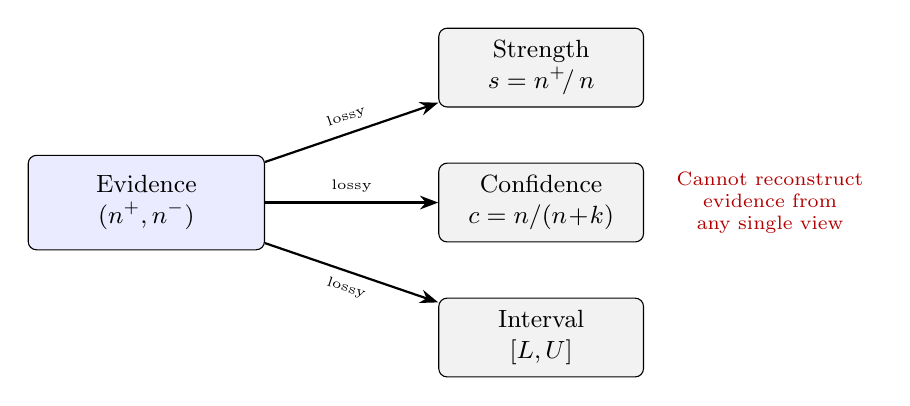
\begin{tikzpicture}[
  >=Stealth, every node/.style={font=\small},
  src/.style={draw, rounded corners=3pt, fill=blue!8, align=center,
              minimum width=30mm, minimum height=12mm},
  tgt/.style={draw, rounded corners=3pt, fill=gray!10, align=center,
              minimum width=26mm, minimum height=10mm},
]
\node[src] (ev) {Evidence\\$(n^+, n^-)$};
\node[tgt, above right=6mm and 22mm of ev] (str)
  {Strength\\$s = n^+\!/\,n$};
\node[tgt, right=22mm of ev] (conf)
  {Confidence\\$c = n/(n\!+\!k)$};
\node[tgt, below right=6mm and 22mm of ev] (itv)
  {Interval\\$[L, U]$};
\draw[->, thick] (ev) -- node[above, font=\tiny, sloped] {lossy} (str);
\draw[->, thick] (ev) -- node[above, font=\tiny] {lossy} (conf);
\draw[->, thick] (ev) -- node[below, font=\tiny, sloped] {lossy} (itv);
\node[font=\scriptsize, text width=26mm, align=center, red!70!black]
  at ($(conf.east) + (16mm, 0)$)
  {Cannot reconstruct\\evidence from\\any single view};
\end{tikzpicture}
\caption{Views of binary evidence are lossy projections.  Each carrier
has its own views (Dirichlet: per-category means; Normal-Gamma:
posterior mean and variance).  No single view reconstructs the
evidence.}
\label{fig:tv-views-projections}
\end{figure}


\section{The Additive / Non-Additive Boundary}

Some projections commute with revision; most do not.  This
distinction determines what can safely be propagated through
inference chains and what cannot.

Total evidence $\mathrm{total}(e) = n^+ + n^-$ is additive:
$\mathrm{total}(e_1 \hplus e_2) = \mathrm{total}(e_1) +
\mathrm{total}(e_2)$.  If you combine two batches of observations,
the total count is the sum of the individual counts.  Total evidence
is an additive shadow---a homomorphism from evidence to
$\mathbb{R}_{\ge 0}^\infty$.

Strength is not additive.  Strength divides positive counts by
total counts---a ratio.  Ratios do not add: a class where 3 out of 4
students passed and a class where 1 out of 4 passed do not combine
to ``4 out of 8 passed'' by adding the ratios $\tfrac{3}{4}$ and
$\tfrac{1}{4}$.  The combined strength is $(3+1)/(4+4) = \tfrac{1}{2}$,
not $\tfrac{3}{4} + \tfrac{1}{4} = 1$.

\begin{theorem}[\code{strength\_not\_additive} (\claimBoundary{})]
There exist $e_1, e_2$ such that
$\mathrm{strength}(e_1 + e_2) \ne
\mathrm{strength}(e_1) + \mathrm{strength}(e_2)$.%
\footnote{Counterexample: $e_1 = (1, 0)$, $e_2 = (0, 1)$.
Formalized in \codepath{Mettapedia/Logic/WorldModelCore.lean}.}
\end{theorem}

\noindent
This is not a deficiency.  It determines the architecture: carry
evidence through inference chains; extract views only at the end.


\section{Simple Truth Values}

A \emph{simple truth value} (STV) is a pair $\langle s, c \rangle$
where $s = n^+ / (n^+ + n^-)$ is the strength and
$c = n / (n + k)$ is the confidence.  It is compact, intuitive,
and lossy: two different evidence values can produce the same STV.%
\footnote{Formalized in
\codepath{Mettapedia/Logic/BinaryEvidence.lean}.}

\maplecourt{%
Querying ``Is the pipe leaking?'' extracts $(1, 4)$: one leak alarm,
four no-alarm readings.  The STV is
$\langle s, c \rangle = \langle 1/5, 5/15 \rangle
= \langle 0.2, 0.33 \rangle$ (with $k = 10$): low confidence in a
low-strength hypothesis.  The fork query ``Is the room occupied?''
extracts $(5, 1)$ with $\langle 0.83, 0.38 \rangle$: higher strength,
similar confidence.  Both views are lossy projections of the same
underlying evidence.  The strength of $(5, 1)$ exceeds that of
$(1, 4)$, but neither STV reveals how many observations contributed
---that information lives in the evidence, not the view.%
\footnote{Proved in
\codepath{artifacts/conformance/maple\_court\_bn\_motifs.metta}
(leak: strength $= 0.2$; fork: strength $\approx 0.833$).}}


\section{Confidence}

Confidence is strictly a derived view:
$c(n^+, n^-) = (n^+ + n^-) / (n^+ + n^- + k)$.  It is monotone in
sample size: more evidence always means higher confidence.  But
confidence says nothing about whether the evidence supports the claim.
A high-confidence negative result is still informative.

\begin{figure}[htbp]
\centering
\includegraphics[width=0.85\textwidth]{../results/figures/confidence_curves.pdf}
\caption{Confidence as a function of sample size for the three
  carriers.  All three are monotone: more evidence always means
  higher confidence.  The PPLBench comparison
  (Chapter~\ref{ch:pplbench}) validates these curves against
  Stan's NUTS sampler.}
\label{fig:confidence-curves}
\end{figure}


\section{Indefinite Truth Values}

An interval $[s_L, s_U]$ bounds the strength.  Three semantics
exist and must not be conflated:

\begin{enumerate}
\item \textbf{Bayesian credible intervals}: posterior probability
  that the true parameter lies in $[s_L, s_U]$ exceeds a threshold.
  Prior-dependent.

\item \textbf{Walley predictive intervals}: derived from the
  Imprecise Dirichlet Model~\cite{Walley1996BagOfMarbles}.
  Prior-free but wider.

\item \textbf{Frequentist confidence intervals}: the true parameter
  lies within them with specified coverage probability over repeated
  sampling.
\end{enumerate}

\noindent
The calculus insists on explicit selector choice: the user declares
which interval semantics is intended, and the system computes
accordingly.  The Walley connection is developed in
Chapter~\ref{ch:evidence}, \S``Walley predictive intervals.''%
\footnote{Formalized in
\codepath{Mettapedia/Logic/PLNIndefiniteTruth.lean}.}


\section{Why Views Are Not Proof Objects}
\label{sec:views-not-proof}

Views are indispensable for practical inference.  But they are not
the right objects to pass between inference steps.  When you chain
two inferences using only the STV of the intermediate result, you
lose information about the posterior shape, the correlation structure,
and the raw counts.

The discipline of the calculus: carry evidence between inference
steps; extract views only at the end, for display or decision.

\paragraph{A concrete illustration: three PLN confidence bugs.}
The MeTTa PLN implementation contains three formally proved
confidence-formula errors that arise precisely from operating on views
instead of evidence:%
\footnote{Formalized:
\codepath{Mettapedia/Logic/PLNBugAnalysis.lean}
(0~sorry, 14~theorems with concrete counterexamples and MeTTa
patches).}

\begin{enumerate}
\item \textbf{Double-damping.}  The induction rule computes
  $\code{w2c}(\min(c_1, c_2))$, applying the
  weight-to-confidence function to a value that is already a
  confidence.  This double-damps: at $c_1 = c_2 = 0.9$, the
  buggy formula gives $0.474$ instead of $0.9$---a 47\%
  underestimate.  The correct formula converts to weights first:
  $\code{w2c}(\min(\code{c2w}(c_1), \code{c2w}(c_2))) =
  \min(c_1, c_2)$.

\item \textbf{Confidence floor.}  The revision rule clamps
  output confidence to $\max(c, c_1, c_2)$.  Under correct
  evidence-based revision, combined confidence always exceeds
  each input (proved), so the clamp is a no-op---but it masks
  bugs elsewhere by hiding negative or nonsensical intermediate
  values.

\item \textbf{Division by zero.}  The function
  $\code{c2w}(c) = c/(1-c)$ diverges at $c = 1$.  In MeTTa,
  this silently returns $\varnothing$.  The MeTTa-level patch
  caps confidence at $\code{MAX\_CONF} < 1$---a reasonable
  engineering approximation with a proved error bound, since
  certainty ($c = 1$) requires infinite evidence and never
  arises in practice.  But the deeper lesson is that
  \code{c2w} is an attempt to invert a lossy projection:
  it recovers weight from confidence, which is the opposite
  of the D4 direction.  The evidence algebra works with
  $(n^+, n^-)$ directly, where the total $n^+ + n^-$
  plays the role of weight without any division or cap.
\end{enumerate}

\noindent
All three bugs disappear when the system works with evidence
pairs rather than confidence scalars.  In weight space (which is
isomorphic to evidence counts via the round-trip
$\code{w2c}(\code{c2w}(c)) = c$, proved), composition is
multiplication; in confidence space, it is not.  This is the
practical consequence of D4 (Evidence over Views): the bugs are not
implementation accidents---they are symptoms of operating on the
wrong abstraction layer.

\begin{quote}
\emph{Probability is what you query; evidence is what you carry.}
\end{quote}

%% ─────────────────────────────────────────────────────────────────

\chapter{Natively Typed World Models}
\label{ch:typed}

Chapter~\ref{ch:world-models} presented the world-model calculus as
an algebraic interface: three operations, five rules in the additive
regime, a $2 \times 2$ refinement square.  This chapter shows that the
same calculus has a \emph{typed rewrite face}: a concrete family of
typed rewrite rules whose terms carry native types and whose reductions
correspond exactly to the algebraic laws.

The point is not to add a second semantics.  It is to make the
calculus \emph{mechanically checkable}: a computer can verify that a
compiled rewrite is sound by reducing it in the typed system.

\section{The Pattern Vocabulary}

The calculus is encoded in three core sorts---\textbf{State},
\textbf{Query}, \textbf{Value}---and constructors corresponding to
the calculus operations:

\medskip
\begin{center}
\begin{tabular}{lll}
\toprule
\textbf{Constructor} & \textbf{Signature} & \textbf{Operation} \\
\midrule
$\mathsf{Revise}(W_1, W_2)$ & State $\times$ State $\to$ State
  & revision \\
$\mathsf{Extract}(W, q)$ & State $\times$ Query $\to$ Value
  & extraction \\
$\mathsf{Combine}(e_1, e_2)$ & Value $\times$ Value $\to$ Value
  & additive fusion \\
$\mathsf{Forget}(S, W)$ & Scope $\times$ State $\to$ State
  & scoped retraction \\
$\mathsf{OverlapMerge}(W_1, W_2)$ & State$^2 \to$ State
  & overlap-aware merge \\
\bottomrule
\end{tabular}
\end{center}
\medskip

\noindent
The remaining constructors---30~total across all extension
families---handle trust-gated revision, source-labeled provenance,
fixpoint closure, order-cost tracking, Kripke modalities, and generic
carriers.  Each appears when the corresponding axis of the 13-axis
family (\S\ref{sec:wm-13axis}) is enabled.  The table above shows the
core that is always present.%
\footnote{Formalized in
\codepath{Mettapedia/OSLF/Framework/WMCalculusBNBridge.lean}.}


\section{The Five Rules as Typed Rewrites}
\label{sec:five-as-rewrites}

The five algebraic rules from \S\ref{sec:algebraic-core} --- the
same five, now expressed as pattern-matching rewrites rather than
algebraic identities:  Each has a typed left-hand
side, a right-hand side, and (for guarded rules) a premise:

\begin{enumerate}
\item $\mathsf{Extract}(\mathsf{Revise}(W_1, W_2), q) \;\leadsto\;
  \mathsf{Combine}(\mathsf{Extract}(W_1, q),\;
  \mathsf{Extract}(W_2, q))$.

\item $\mathsf{Revise}(W_1, W_2) \;\leadsto\;
  \mathsf{Revise}(W_2, W_1)$.

\item $\mathsf{Revise}(\mathsf{Revise}(W_1, W_2), W_3)
  \;\leadsto\; \mathsf{Revise}(W_1, \mathsf{Revise}(W_2, W_3))$.

\item $\mathsf{Combine}(e_1, e_2) \;\leadsto\;
  \mathsf{Combine}(e_2, e_1)$.

\item $\mathsf{Combine}(e, \mathsf{Zero}) \;\leadsto\; e$.
\end{enumerate}

\noindent
All five derive from the single condition that $\mathsf{Extract}$ is
an additive monoid homomorphism.  The Lean formalization encodes each
as a \code{RewriteRule} with typed metavariables, premises, and
left/right patterns.  Sixteen step lemmas are kernel-checked across
the core and extension axes.%
\footnote{Formalized in
\codepath{Mettapedia/OSLF/Framework/WMCalculusLanguageDef.lean}.}


\section{The \texorpdfstring{$2 \times 2$}{2x2} Calculus Square
  as Concrete Rewrites}

Two orthogonal refinements produce four variant calculi:

\begin{center}
\begin{tabular}{lll}
\toprule
& \textbf{Plain} & \textbf{+ Congruence} \\
\midrule
\textbf{Raw} & all rules fire & + descent into subterms \\
\textbf{Guarded} & side-condition oracle & + descent into subterms \\
\bottomrule
\end{tabular}
\end{center}

\noindent
The raw calculus overapproximates the guarded one: dropping premises
only enables more reductions.  The congruence extension adds
15~explicit rules enabling reductions to propagate into subterms.
All four inclusion arrows and Galois connections
$\Diamond \dashv \Box$ are kernel-checked.%
\footnote{Formalized in
\codepath{Mettapedia/OSLF/Framework/WMCalculusContextClosure.lean}.}

The congruence infrastructure enables multi-step decomposition under
context.  For example, the term
$\mathsf{Extract}(\mathsf{Revise}(\mathsf{Revise}(W_1, W_2), W_3), q)$
reduces in two steps to
$\mathsf{Combine}(\mathsf{Combine}(\mathsf{Extract}(W_1, q),
\mathsf{Extract}(W_2, q)), \mathsf{Extract}(W_3, q))$:
the first step applies evidence-add at the top; the second uses a
congruence rule to apply evidence-add \emph{inside} the left
$\mathsf{Combine}$ argument.


\section{Intrinsic Encoding and Adequacy}

The central fact: the typed calculus and the pattern-level calculus
agree exactly.  A reduction holds at the abstract level if and only
if the corresponding pattern-level reduction holds on the encoded
terms.

The abstract syntax is an intrinsically sorted type family
$\mathsf{WMTerm} : \mathsf{WMSort} \to \mathsf{Type}$ with three
sorts.  A computable encoding $\mathsf{encodeWM}$ maps abstract
terms to the OSLF pattern language.

\begin{theorem}[Biconditional adequacy (\claimCore{})]
A reduction at the abstract $\mathsf{WMTerm}$ level holds if and only
if the corresponding pattern-level OSLF reduction holds on the encoded
terms.  The two presentations agree exactly.%
\footnote{Formalized: \code{wmStep\_iff} (single step),
\code{wmStepStar\_adequate} (multi-step), both kernel-checked.
See \codepath{Mettapedia/OSLF/Framework/WMCalculusEncoding.lean}.}
\end{theorem}

\noindent
The encoding is injective within each sort.  Subject reduction is
definitional: every constructor of $\mathsf{WMStep}$ preserves the
sort by construction.

For the $\Box$ modality, backward completeness holds when restricted
to the image of $\mathsf{encodeWM}$:

\begin{center}
\begin{tabular}{lcc}
\toprule
& Forward ($\Diamond$) & Backward ($\Box$) \\
\midrule
Unrestricted & biconditional & sound only \\
Image-restricted & biconditional & biconditional \\
\bottomrule
\end{tabular}
\end{center}


\section{The 13-Axis Vertex Family}
\label{sec:wm-13axis}

The full typed family is indexed by 13 orthogonal axes.  The first
four control semantic interpretation without changing the rewrite
rules; the remaining nine each add genuinely new rules to the
calculus:

\begin{center}
{\footnotesize
\begin{tabular}{rlll}
\toprule
\textbf{\#} & \textbf{Axis} & \textbf{Values} & \textbf{Effect} \\
\midrule
1--4 & Base (logic, tv, interval, typing)
     & $24$ combinations & model-level (same rules) \\
5 & Overlap & additive $|$ overlapAware & +1 rule \\
6 & Forgetting & none $|$ scopeBased $|$ tracked & +2--3 rules \\
7 & Provenance & none $|$ sourceLabeled & +6 rules \\
8 & Fixpoint & none $|$ closure $|$ policy & +2--4 rules \\
9 & Cost & none $|$ costTracked & +3 rules \\
10 & Conservation & none $|$ conserving & +2 rules \\
11 & Experiment & none $|$ stochastic & +3--7 rules \\
12 & Kripke & none $|$ pointedKripke & +3 rules \\
13 & Carrier & concrete $|$ generic & +2 rules \\
\bottomrule
\end{tabular}}
\end{center}

\noindent
The first four axes are model-level: all 24~combinations produce the
same rewrite rules.  The remaining nine are syntactic: each adds new
rules.  The minimal vertex (all extensions off) has 5~rules; the
maximal vertex has 36.%
\footnote{Formalized in
\codepath{Mettapedia/OSLF/Framework/TypeSynthesis.lean}.}

\maplecourt{%
Maple Court's apartment WM sits at a mid-range vertex: overlap-aware
(sensors may share a vent), scope-based forgetting (stale readings
expire), source-labeled provenance (which sensor contributed).  The
building WM adds cost tracking (order-cost governance for the cleaning
robot's schedule).  Each vertex determines which rewrite rules are
available---and which side conditions must be checked.}

\noindent
The 4-vertex WM regime classification
(\S\ref{sec:non-additive}) maps injectively into the 13-axis
family: each regime determines specific axis settings
(commutativity, derived-additivity, probabilistic
interpretation).%
\footnote{Formalized in
\codepath{Mettapedia/Logic/ModalProbabilityBridge.lean}
(14~items, 0~sorry).}


\section{OSLF Modal Operators and Semantic Bridge}

From any vertex's \code{LanguageDef}, the OSLF framework automatically
derives modal operators $\Diamond$ (forward reachability: ``some
reduction leads to a state satisfying $\varphi$'') and $\Box$
(backward invariance: ``every predecessor satisfies $\varphi$'') with
a Galois connection $\Diamond \dashv \Box$.

This is not optional decoration.  The modal operators give the typed
calculus its semantic backbone: $\Diamond$ captures what can be
derived; $\Box$ captures what is preserved.  The Galois connection
ensures the two are dual.%
\footnote{The construction follows
Meredith's~\cite{meredith2026ccc} context-decorated HML modalities,
derived from the GSLT's operational semantics.}

Diamond theorems, relational encoding, evidence barbs
(process-algebraic observables), neighborhood semantics, and
first-order logic all arise as semantic fibers of this construction.


\section{Native Type Synthesis}

The native-type-theorem (NTT) pass extracts, for each vertex, the
type that classifies its allowable terms and reductions.  The pass is
exact on 9~syntactic axes and intentionally insensitive to
4~model-level axes.%
\footnote{Formalized: \code{wmVertexNativeType\_eq} (kernel-checked).}

Native types do not introduce a second semantics.  They expose, at
the rewrite level, the structural behavior already present in the
semantic kernel.  A term that type-checks at a given vertex is
guaranteed to reduce according to that vertex's rules.


\section{World Models from GSLTs}
\label{sec:gslt-wm}
\label{sec:gslt-open-program}

For any type~$T$, multiset ensembles of~$T$ form a world model when
queried by decidable properties: extraction counts satisfying and
refuting entities, and the count is additive over multiset union.

\begin{theorem}[\code{universalEnsembleWorldModel} (\claimCore{})]
For any type~$T$:
$\code{AdditiveWorldModel}\;(\code{Multiset}\;T)\;(\code{DecProp}\;T)$.%
\footnote{Formalized in
\codepath{Mettapedia/OSLF/Framework/GSLTWorldModel.lean}.
Existence and uniqueness for any observation type $\times$
evidence carrier are packaged in
\codepath{Mettapedia/Logic/UniversalEnsembleWM.lean}
(7~items, 0~sorry).}
\end{theorem}

\noindent
This means: every computational system with parallel
composition---every graph-structured lambda theory (GSLT) in
Meredith's~\cite{meredith2026ccc} sense---has a canonical additive
world model via multiset counting.  The converse also holds: a
GSLT equipped with an additive evidence assignment IS an
\code{AdditiveWorldModel}, with the GSLT's weight map as the
\code{extract} function and forward transport (reductions in
weaker theories lift to stronger ones) as \code{extract\_add}.%
\footnote{Formalized in
\codepath{Mettapedia/Logic/GSLTWeightMapBridge.lean}
(7~items, 0~sorry).}

\begin{conjecture}[WM universality for typed rewrite systems]
The WM calculus is not specific to probabilistic logic; it is the
natural evidence framework for any typed rewrite system.  Every
\code{LanguageDef} (i.e., every vertex
of the typed family) gives an additive world model via the
OSLF-derived modal operators.  Replacing $V$ with $\mathbb{C}$ gives
Meredith's amplitude framework; replacing $V$ with
$\mathbb{R}_{\ge 0}^\infty$ gives the Knuth--Skilling probability
framework.  The probability
hypercube~\cite{StayWells2026} classifies theories by which
combination of merge-law and carrier properties they satisfy
(Chapter~\ref{ch:future}).
\end{conjecture}
%
\footnote{Open program: the full LanguageDef $\to$ AdditiveWorldModel
construction, the StatefulValuation typeclass unifying state-side and
obs-side laws, and the grand theorem connecting WM + KS + Meredith as
specializations of one bivariate extractor.  A work-in-progress Lean formalization
of the probability hypercube axes (commutativity, distributivity,
precision, additivity, etc.) exists across 29~files in
\codepath{Mettapedia/ProbabilityTheory/Hypercube/}.}

The philosophical import of this direction is worth pausing on.
If the conjecture holds, then the world-model calculus is not a
tool designed for one application.  It is the structure that
\emph{any} typed rewrite system naturally acquires when you ask it
to track evidence about its own behavior.  A Bayesian network, a
process calculus, a programming language, a causal model---each
would have its own canonical world model, the same way each has its
own type system.  Evidence extraction would be as natural and
universal as type-checking.

The typed calculus constructs world models.  The next chapter shows
what even the best local construction cannot achieve.

%% ─────────────────────────────────────────────────────────────────

\chapter{The No-Go Theorem}
\label{ch:no-go}

The previous chapters built the calculus, its evidence carriers, its
state operations, its views, and its typed realization.  This chapter
establishes the fundamental limit of the framework: what even the most
expressive local computation cannot achieve.

One might hope for a function that takes local per-link evidence and
computes complete evidence for any derived query.  No such function
exists.

\begin{theorem}[No local complete deduction rule (\claimBoundary{})]
\label{thm:no-go}
There is no function $f : V^5 \to V$ that, for all joint evidence
states~$E$, computes the exact link evidence for $A \Rightarrow C$
from only the local premises $\mathrm{extract}(E, A)$,
$\mathrm{extract}(E, B)$, $\mathrm{extract}(E, C)$,
$\mathrm{extract}(E, A \!\Rightarrow\! B)$,
$\mathrm{extract}(E, B \!\Rightarrow\! C)$.%
\footnote{Formalized in
\codepath{Mettapedia/Logic/PLNJointEvidenceNoGo.lean}.}
\end{theorem}

\begin{proof}[Proof sketch]
For three atoms, construct two joint states $E_1, E_2$ that agree on
all five local marginals but disagree on $A \Rightarrow C$.  The key:
among the four worlds where $A = 1$, the entries for
$(A\!=\!1, B\!=\!0, C\!=\!1)$ and $(A\!=\!1, B\!=\!1, C\!=\!0)$ can be
traded against each other.  Concretely, transfer mass~$\epsilon$
from world $(1,0,1)$ to world $(1,1,0)$.  Both worlds have $A = 1$,
so the $\mathrm{ev}(A)$ marginal is unchanged.  The first contributes
to $B\!=\!0$ and the second to $B\!=\!1$, but by equal amounts, so
$\mathrm{ev}(B)$ is unchanged.  Likewise for $\mathrm{ev}(C)$ (the
first has $C\!=\!1$, the second $C\!=\!0$).  The link marginals
$\mathrm{ev}(A\!\Rightarrow\!B)$ and $\mathrm{ev}(B\!\Rightarrow\!C)$
each sum over one column and one row of the $B \times C$ sub-table
given $A\!=\!1$; the trade shifts mass within each row and column by
equal amounts, preserving both sums.  But $\mathrm{ev}(A\!\Rightarrow\!C)$
counts the worlds where $A\!=\!1$ and $C\!=\!1$: the trade removes one
such world and adds none, directly changing this marginal.
\end{proof}

\begin{figure}[htbp]
\centering
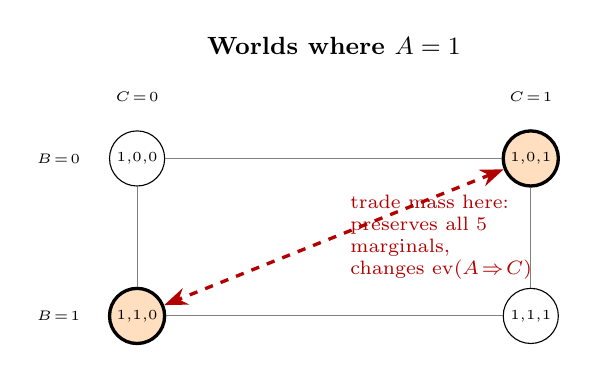
\begin{tikzpicture}[
  >=Stealth, every node/.style={font=\scriptsize},
  world/.style={draw, circle, minimum size=7mm, inner sep=1pt},
  swap/.style={draw, circle, minimum size=7mm, inner sep=1pt,
               fill=orange!25, very thick},
]
\node[font=\small\bfseries, anchor=south] at (2.5, 3.2)
  {Worlds where $A=1$};
\node[world] (w100) at (0, 2) {$\scriptscriptstyle 1,0,0$};
\node[swap]  (w101) at (5, 2) {$\scriptscriptstyle 1,0,1$};
\node[swap]  (w110) at (0, 0) {$\scriptscriptstyle 1,1,0$};
\node[world] (w111) at (5, 0) {$\scriptscriptstyle 1,1,1$};
\draw[thin, gray] (w100) -- (w101);
\draw[thin, gray] (w100) -- (w110);
\draw[thin, gray] (w101) -- (w111);
\draw[thin, gray] (w110) -- (w111);
\draw[<->, very thick, red!70!black, dashed]
  (w101) -- node[right=2pt, font=\scriptsize, text width=28mm,
  align=left] {trade mass here:\\preserves all 5 marginals,\\
  changes $\mathrm{ev}(A\!\Rightarrow\! C)$} (w110);
\node[font=\tiny, anchor=east] at (-0.6, 2) {$B\!=\!0$};
\node[font=\tiny, anchor=east] at (-0.6, 0) {$B\!=\!1$};
\node[font=\tiny, anchor=south] at (0, 2.6) {$C\!=\!0$};
\node[font=\tiny, anchor=south] at (5, 2.6) {$C\!=\!1$};
\end{tikzpicture}
\caption{The no-go witness.  Redistributing mass between the orange
worlds preserves all five local marginals but changes
$\mathrm{ev}(A \Rightarrow C)$.}
\label{fig:no-go-witness}
\end{figure}

\noindent
This theorem does not make fast inference useless.  It tells us what
fast inference \emph{cannot claim}: completeness for arbitrary world
models without structural assumptions.  The constructive response:
\begin{enumerate}
\item Restrict the model class (BN factorization makes local
  computation exact --- Chapter~\ref{ch:bn-models}).
\item State the assumptions (every compiled rule carries its $\Sigma$).
\item Provide corrected alternatives where original rules required
  unstated assumptions.
\end{enumerate}

\maplecourt{%
Two BN structures for Maple Court give the same per-link marginals
$P(\text{leak})$ and $P(\text{humidity})$ but different
$P(\text{mold} \mid \text{humidity}, \text{leak})$.  No amount of
per-link evidence distinguishes them.  The BN DAG structure --- a
side condition $\Sigma$ --- is what breaks the degeneracy.}

\noindent
The constructive resolution of this limitation---distributional
inference, certified chaining bounds, and view transport---appears
in Chapter~\ref{ch:error-transport}.


%% ═══════════════════════════════════════════════════════════════════
\part{Compiled Inference, Scale, and Control}
\label{part:compiled}
%% ═══════════════════════════════════════════════════════════════════

\chapter{\texorpdfstring{$\Sigma$}{Sigma}-Guarded Rewrites}
\label{ch:sigma-rewrites}

The no-go theorem says local chaining cannot be complete in general.
This chapter gives the constructive response: \emph{compiled
rewrites} that are exact under explicit structural assumptions.  A
compiled rewrite is not new semantics.  It is a certified shortcut to
an answer already determined by the underlying world model.

\section{The Rewrite Pattern}

A $\Sigma$-guarded rewrite has the form: given that side condition
$\Sigma$ holds (BN factorization, screening-off, positivity), the
rewrite computes the \emph{same} value as the full posterior query.
The rule is a theorem, not a heuristic.

\[
\frac{\Sigma \vdash \mathrm{ScreenOff}(A, B, C) \quad
      \Sigma; \Gamma \vdash \mathrm{link}(A, B) \Downarrow e_{AB}
      \quad \cdots}
     {\Sigma; \Gamma \vdash \mathrm{link}(A, C) \Downarrow e_{AC}}
\]

\noindent
The side condition $\Sigma$ is not optional.  When it fails, the
rule does not apply.  The system falls back to the full posterior.%
\footnote{Formalized in
\codepath{Mettapedia/Logic/PLNBayesNetFastRules.lean} and
\codepath{Mettapedia/Logic/PLNDerivation.lean}.}

\section{The Compiled Rule Catalog}

Each compiled rule has a name, a pattern, a side condition $\Sigma$,
a strength formula, and a correctness theorem.  The catalog:

\medskip
{\footnotesize
\begin{center}
\begin{tabular}{llll}
\toprule
\textbf{Rule} & \textbf{Pattern} & \textbf{$\Sigma$}
  & \textbf{Strength formula} \\
\midrule
Deduction & $A \!\to\! B \!\to\! C$
  & screening-off, positivity
  & $s_{AB} s_{BC} + (1\!-\!s_{AB})\frac{s_C - s_B s_{BC}}{1 - s_B}$ \\[3pt]
Induction & $C \!\to\! A,\; C \!\to\! B$
  & screening-off
  & $s_{AB} \!=\! \frac{s_{BA} s_B}{s_A}$; then deduction \\[3pt]
Abduction & $A \!\to\! C,\; B \!\to\! C$
  & screening-off
  & $s_{BC} \!=\! \frac{s_{CB} s_C}{s_B}$; then deduction \\[3pt]
Modus ponens & $A,\; A \!\Rightarrow\! B$
  & none
  & $s_{AB} \cdot s_A + (1\!-\!s_A) \cdot c$ \\[3pt]
Revision & $e_1, e_2$
  & stamp-disjoint
  & weighted average of $s_1, s_2$ \\[3pt]
Negation & $A$
  & none
  & $1 - s_A$ \\[3pt]
Inversion & $A \!\to\! B$
  & none
  & $s_{BA} \!=\! s_{AB}$;\; $c_{BA} \!=\! c_{AB} \!\cdot\! \tfrac{n_A}{n_B}$ \\
\bottomrule
\end{tabular}
\end{center}}
\medskip

\noindent
These are the classical PLN rules of Goertzel et
al.~\cite{goertzel2009pln}, now with explicit side conditions and
kernel-checked correctness proofs.  The deduction formula is exact
under the chain BN structure with screening-off and positivity
($0 < s_B < 1$)---see Theorem~\ref{thm:chain-deduction}.
Induction and abduction are
Bayes-inversions of deduction, with their own screening-off
conditions.  Revision is evidence addition
(\S\ref{sec:additive-regime}).%
\footnote{Formalized in \codepath{Mettapedia/Logic/PLNDerivation.lean}
(strength formulas, bounds, and Bayes-inversion theorems) and
\codepath{Mettapedia/Logic/PLNBayesNetFastRules.lean} (BN exactness
theorems).}

\section{Compiled Tactics vs.\ Foundational Semantics}

The distinction is crucial: the kernel (Part~II) says what the answer
\emph{is}.  Compiled shards say how to compute it \emph{fast}.  If
the side condition is met, the shard gives the exact answer.  If not,
the system falls back to the full extraction.

The $\Sigma$-discipline ensures that every shortcut is explicitly
licensed.  A rule either has a proof of correctness under $\Sigma$,
or it is not available.

For maximum fidelity, propagate the full posterior distribution
through the chain rather than scalar summaries.  The distributional
approach avoids the variance accumulation that scalar chaining
inevitably introduces (Chapter~\ref{ch:error-transport}).  Scalar
chaining is a useful further approximation within the distributional
framework, not a replacement for it.

%% ─────────────────────────────────────────────────────────────────

\chapter{Bayesian-Network Exactness}
\label{ch:bn-models}

The original PLN rule family --- deduction, induction, abduction,
revision, modus ponens --- was designed by Goertzel, Iklé, Goertzel,
and Heljakka~\cite{goertzel2009pln} as a general-purpose uncertain
reasoner.  Geisweiller's \nuPLN{} framework~\cite{nuPLN2026} grounded
the evidence representation in de~Finetti's exchangeability theorem.
This chapter shows that the classical rules become \emph{exact}
compiled rewrites when the world model has Bayesian-network structure
--- not approximate heuristics, but certified shortcuts with explicit
side conditions.

\section{BN World-Model Class}

A Bayesian-network world model consists of a DAG specifying the
factorization plus local conditional probability tables (CPTs) carrying
evidence counts.  Revision is addition of local counts (conjugate
updating); query answering proceeds by exact inference.  The DAG
structure provides the $\Sigma$ that chain/fork/collider rules
require.%
\footnote{Formalized in
\codepath{Mettapedia/Logic/PLNBayesNetWorldModel.lean}.}


\section{Exact BN Query Bridge}

BN queries correspond to posterior marginalization.  The central
fact is a commutative diagram: a BN query answered by variable
elimination agrees with the general world-model extraction applied
to the same state.

\begin{theorem}[BN query bridge (\claimCore{})]
For a BN world-model class with DAG~$G$ and evidence state~$W$,
\[
  \mathrm{extract}_{\mathrm{BN}}(W, q) = \mathrm{extract}_{\mathrm{WM}}(W, q)
\]
for every query~$q$ in the scope of the BN.%
\footnote{Formalized:
\code{bnQueryBridge\_extraction\_eq} in
\codepath{Mettapedia/Logic/PLNBayesNetWorldModel.lean}.}
\end{theorem}

\noindent
The BN structure does not change the answer---it changes the
\emph{cost} of obtaining it.  Without the DAG, answering a query
requires summing over all $2^n$ worlds.  With the DAG, variable
elimination factors the sum into local operations whose cost is
exponential only in the treewidth.  The answer is the same;
the computational path is shorter.


\section{Chain, Fork, and Collider Exactness}

The three fundamental BN motifs each yield exactness theorems.
We derive the chain case in full; the fork and collider cases
follow the same pattern with their own side conditions.

\paragraph{Deriving the deduction formula.}
Start from the law of total probability:
\[
  P(C \mid A) = P(C \mid A, B)\,P(B \mid A)
              + P(C \mid A, \neg B)\,P(\neg B \mid A).
\]
Under the screening-off assumption $P(C \mid A, B) = P(C \mid B)$
and $P(C \mid A, \neg B) = P(C \mid \neg B)$, this simplifies to:
\[
  P(C \mid A) = P(C \mid B)\,P(B \mid A)
              + P(C \mid \neg B)\,(1 - P(B \mid A)).
\]
Writing $s_{AB} = P(B \mid A)$, $s_{BC} = P(C \mid B)$,
$s_B = P(B)$, $s_C = P(C)$, and eliminating $P(C \mid \neg B)$
via $s_C = s_B \cdot s_{BC} + (1 - s_B) \cdot P(C \mid \neg B)$:

\begin{definition}[PLN deduction strength]
\label{def:deduction-strength}
\[
  \mathrm{plnDed}(s_{AB}, s_{BC}, s_B, s_C) :=
  s_{AB} \cdot s_{BC}
  + (1 - s_{AB}) \cdot \frac{s_C - s_B \cdot s_{BC}}{1 - s_B}
\]
defined when $0 < s_B < 1$.
\end{definition}

\noindent
This formula was introduced by Goertzel et
al.~\cite{goertzel2009pln} and is derived here from first principles
under the screening-off assumption.

\begin{theorem}[Chain BN deduction exactness (\claimConditional{})]
\label{thm:chain-deduction}
For a chain BN $A \to B \to C$ with positivity ($0 < s_B < 1$) and
screening-off:
\[
  \mathrm{strength}(W, \mathrm{link}(A, C)) =
  \mathrm{plnDed}(s_{AB}, s_{BC}, s_B, s_C).
\]%
\footnote{Formalized: \code{chainBN\_plnDeductionStrength\_exact}
in \codepath{Mettapedia/Logic/PLNBayesNetFastRules.lean}.}
\end{theorem}

\noindent
The analogous result holds for fork BNs
$A \leftarrow B \to C$.%
\footnote{Formalized:
\code{forkBN\_plnDeductionStrength\_exact}.}

\paragraph{Induction and abduction.}
Both reduce to Bayes-inversion followed by deduction.
\emph{Induction}: given $P(A \mid B)$ and $P(A \mid C)$, estimate
$P(C \mid B)$.  First invert:
$s_{AB} = s_{BA} \cdot s_B / s_A$ (Bayes's theorem), then apply
the deduction formula with $s_{AB}$.
\emph{Abduction}: given $P(B \mid A)$ and $P(B \mid C)$, estimate
$P(A \mid C)$.  Invert:
$s_{BC} = s_{CB} \cdot s_C / s_B$, then deduction.%
\footnote{Formalized in
\codepath{Mettapedia/Logic/PLNDerivation.lean}:
\code{plnInduction\_eq\_bayes\_deduction},
\code{plnAbduction\_eq\_bayes\_deduction}.}

The chain theorem above is stated at the strength (scalar) level.
At the \emph{distributional level}, the story is cleaner: propagate
the full Beta or Dirichlet posterior through the chain, and the
result is exact under d-separation---no variance accumulation, no
information loss.  The scalar deduction formula is the strength
\emph{view} of this distributional chain.  The five
chaining-limitation theorems of Chapter~\ref{ch:error-transport}
make the cost of the scalar approximation precise; the distributional
dominance theorem (ibid.) shows that carrying the full posterior is
strictly more informative.

\maplecourt{%
The chain $\mathrm{PipeLeak} \to \mathrm{WallHumidity} \to
\mathrm{MoldRisk}$ in Maple Court: the compiled chain rule computes
$P(\text{mold} \mid \text{leak})$ from the per-link evidence under
the BN factorization.  The side condition: $\mathrm{WallHumidity}$
screens off $\mathrm{MoldRisk}$ from $\mathrm{PipeLeak}$.  When
this holds, the compiled answer is exact.  When it fails (e.g., a
direct leak-to-mold pathway exists), the rule is not licensed.}


\section{Class-Packaged BN Discharge}

One of the practical payoffs of the $\Sigma$-discipline is that
side-condition checking can be automated.  For discrete BNs with
explicit CPTs, the function
\code{allDiscreteCPTLocalMarkov\_of} verifies d-separation and
screening-off for every pair of non-adjacent nodes---i.e., it
checks the local Markov property.  If the check passes, all the
chain, fork, and collider exactness theorems are simultaneously
unlocked for that model.  The BN DAG structure itself constitutes
the proof of the side condition.%
\footnote{Formalized in
\codepath{Mettapedia/Logic/PLNBayesNetWorldModel.lean}.}


\section{Worked Proof-Carrying Contraction}

A binary BN $A \leftarrow H \to B \to C \to D$ demonstrates the full
discipline.  Positive control: the chain fires correctly with
$P(B \mid A) \approx 0.615$.  Negative control~1: the soft gate
fails when d-separation is violated.  Negative control~2: collider
naive abduction fails.  The negative controls are as important as
the positive ones --- they show that the $\Sigma$-discipline catches
real errors.%
\footnote{Formalized in
\codepath{Mettapedia/Logic/PLNProofCarryingContractionDemo.lean}.}


\section{PLN v0.9 Examples as Compiled WM Instances}

PLN v0.9~\cite{goertzel2009pln}\footnote{PLN v0.9:
\texttt{github.com/trueagi-io/PLN}, tag \texttt{v0.9}.} provides
three flagship examples exercising the classical rule family.  Each
is a compiled BN rewrite with provenance tracking:

\begin{description}
\item[DeductionRevision.]  Two chains $A \to B \to D$ and
  $A \to C \to D$ with disjoint stamps $\{0,2\}$ and $\{1,3\}$;
  revision is safe; forgetting obs~0 preserves path~2.

\item[RavenInduction.]  Induction from two ravens' data; forgetting
  rv2 reduces the induction to rv1's evidence alone.

\item[FlyingRaven.]  Chain Sam$\to$Raven$\to$Bird$\to$flies vs.\
  Pingu$\to$Penguin$\to\neg$flies; forgetting Sam$\to$Raven
  conserves Pingu.
\end{description}

\noindent
All verified with 20~kernel-checked conformance tests.%
\footnote{Formalized in
\codepath{Mettapedia/Logic/PLNClassicExamples.lean}.}

The stepped walkthrough for DeductionRevision with provenance
appears in Chapter~\ref{ch:state-ops},
\S\ref{sec:pln-stamps} --- including both tikz diagrams
(Figure~\ref{fig:deduction-revision-stamps} and
Figure~\ref{fig:deduction-revision-forget}).


\section{Bridge Theorems: Naive Bayes and k-NN}
\label{sec:bridge-nb-knn}

Two standard ML classifiers are exact world-model instances.

\paragraph{Naive Bayes.}
A Naive Bayes classifier with class variable~$C$ and features
$F_1, \ldots, F_n$ is a BN fork: $C \to F_1, \ldots, C \to F_n$.
Classification amounts to querying
$\arg\max_c \,\mathrm{extract}(W, c)$ where the evidence for class~$c$
is the tensor product of per-feature evidences
$\bigotimes_{i=1}^n e_{F_i \mid c}$.  The conditional-independence
assumption of Naive Bayes IS the d-separation condition of the fork BN.

\paragraph{$k$-Nearest Neighbors.}
$k$-NN is evidence-weighted revision: the $k$ nearest neighbors each
contribute an evidence fragment $e_i$ (one observation of the target
class), and the prediction is the extraction from their sum
$e_1 \hplus \cdots \hplus e_k$.  The ``nearest'' selection is a scope
restriction (only the $k$ closest sources revise the state).%
\footnote{Formalized in
\codepath{Mettapedia/Logic/PLNBayesNetInference.lean}.}

\noindent
These are exact bridges, not analogies: the standard ML classifiers
are world-model instances under specific BN structure.  This means
the entire $\Sigma$-discipline applies to them: provenance tracking,
forgetting, conservation, and distributional inference all carry
over.


\section{Factor Graphs: Semantic vs.\ Operational}

A factor graph represents a world-model state by decomposing it into
local factors.  Two readings must be distinguished:

\begin{description}
\item[Semantic factors.] The factors \emph{are} the model.  Each factor
  stores an evidence table (a local CPT enriched with counts), and the
  global state is their product.  This is the BN world-model class
  (\S\ref{sec:additive-regime}).

\item[Operational factors.] The factors are rule schemas.  Message
  passing on the factor graph implements variable elimination, and each
  message corresponds to a partial extraction.
\end{description}

\noindent
The alignment is via compilation: each operational factor corresponds
to a conditional in the semantic model, and the message-passing result
agrees with the full extraction applied to the same state.  The BN
structure is the $\Sigma$ that licenses this agreement.%
\footnote{Formalized:
\code{factorGraphBridge\_extraction\_comm} in
\codepath{Mettapedia/Logic/PLNBayesNetInference.lean}.}

%% ─────────────────────────────────────────────────────────────────

\chapter{Error, Thresholds, and Distributional Resolution}
\label{ch:error-transport}

Scalar chaining---propagating strength and confidence through
inference steps---is the fast path.  This chapter explains why it
is also the lossy path, and what the alternative is.

\section{Certified Chaining: Fundamental Limitations}

Five proved theorems characterize the boundary of scalar chaining.
Each is unconditional: no side condition removes the limitation when
chaining at the scalar (view) level rather than the distributional
(carrier) level.

\begin{enumerate}
\item \textbf{Variance accumulation.}  For a chain of $n$ steps each
  involving an unresolved regime mixture with per-step variance
  $\ge \delta$, the total accumulated variance is
  $\ge n \cdot \delta$.  Variance grows at least linearly.%
  \footnote{Formalized in
  \codepath{Mettapedia/Logic/PLNVarianceChainNoGo.lean}.}

\item \textbf{Sensitivity amplification.}  If each step is
  $K$-Lipschitz, composing $n$ steps yields a $K^n$-Lipschitz chain.
  For $K > 1$, errors amplify exponentially.%
  \footnote{Formalized in
  \codepath{Mettapedia/Logic/PLNSensitivityNoGo.lean}.}

\item \textbf{Coverage collapse.}  If each step has per-step
  coverage at most $1 - \alpha$, the joint coverage decays as
  $(1 - \alpha)^n \to 0$.  Certified per-step guarantees do not
  compose into chain-length-independent certificates.%
  \footnote{Formalized in
  \codepath{Mettapedia/Logic/PLNCoverageCollapseNoGo.lean}.}

\item \textbf{Topology-CPT gap.}  For a BN with fixed DAG topology,
  the conditioning residual can vary arbitrarily across CPT
  parameterizations.  No function of the topology alone bounds
  it non-trivially.%
  \footnote{Formalized in
  \codepath{Mettapedia/Logic/PLNTopologyCPTNoGo.lean}.}

\item \textbf{No universal error bound.}  There is no function of
  the number of chaining steps that bounds the error for all world
  models.  The error depends on the specific joint structure, which
  is exactly what scalar chaining discards.
\end{enumerate}

\noindent
Together these say: information is lost when you project before you
chain.  Each theorem identifies a different mechanism of loss ---
variance, sensitivity, coverage, topology, or structure --- but they
all point to the same conclusion: carry the full posterior.

\section{Distributional Inference: The Constructive Resolution}

The fix: propagate the full posterior distribution through the chain,
not scalar views.  Instead of extracting a strength summary $s = 0.2$
and passing it forward, pass the full $\text{Beta}(2, 5)$
posterior---corresponding to Maple Court's pipe-leak evidence $(1, 4)$
under a $\text{Beta}(1, 1)$ prior.  The next step conditions on the
distribution, not the point estimate.

\begin{theorem}[Distributional dominance (\claimCore{})]
Distributional chaining dominates scalar chaining in information
content.  After $k$ steps, the distributional chain preserves the
full posterior shape, while the scalar chain has accumulated artificial
precision.%
\footnote{Formalized in
\codepath{Mettapedia/Logic/PLNDistributionalConvergence.lean}.}
\end{theorem}

\noindent
This is why the evidence carrier family (Chapter~\ref{ch:evidence})
matters: the carriers store full sufficient statistics, not just
strengths.  Distributional chaining uses those statistics directly.
Scalar chaining projects them to views first, losing information at
each step.

The five limitation theorems and the dominance theorem together say:
\emph{carry the posterior, not the point estimate.}  Or, recalling
Chapter~\ref{ch:views}: \emph{probability is what you query;
evidence is what you carry.}  Scalar views are for display and
decision at the end of a chain, not for intermediate computation.

\section{View Transport Under Query Equivalence}

When two queries are semantically equivalent (same extraction on
every state), their views transport.  This is a corollary of the
universal property: equivalent queries extract the same value, so
every view agrees.

\section{Threshold Semantics}

Truth thresholds ($\mathrm{strength} > 0.5$,
$\mathrm{confidence} > 0.8$) are predicates on views, not on
evidence.  The threshold semantics connects the view layer to
decision-making: an agent acts when the view crosses a threshold.
The calculus makes explicit that thresholds are \emph{policy}, not
\emph{semantics}---changing the threshold changes the decision
boundary, not the underlying evidence.

This has a practical consequence for chaining.  A chain of $n$
compiled rewrites, each passing only scalar views to the next step,
accumulates artificial precision: the output strength \emph{looks}
like a single number, but its actual uncertainty is wider than
what the confidence figure suggests.  The five limitation theorems
above quantify this.  The distributional approach avoids the
problem entirely: the posterior shape carries its own uncertainty,
and thresholds applied to the \emph{final} distributional answer
have calibrated coverage.

\maplecourt{%
The building's mold-risk policy fires when
$\mathrm{strength}(\mathrm{MoldRisk}) > 0.3$ and
$\mathrm{confidence} > 0.5$.  With the pipe-leak chain
$\mathrm{PipeLeak} \to \mathrm{WallHumidity} \to
\mathrm{MoldRisk}$, a scalar chain might report
$s = 0.35$, $c = 0.7$---above threshold.  But
distributional propagation reveals that the $90\%$ credible interval
for the mold-risk posterior spans $[0.1, 0.6]$, so the decision is
less certain than the scalar view suggests.  The threshold decision
remains the same, but the system can now report \emph{how certain}
the threshold crossing is.}

%% ─────────────────────────────────────────────────────────────────

\chapter{Large-Scale Inference and Inference Control}
\label{ch:scale-control}

The previous chapters built a calculus that is correct: states carry
evidence, extraction is additive, compiled rewrites are exact under
explicit side conditions.  This chapter addresses the problem that
correctness alone does not solve: \emph{which correct steps should a
system take?}

A world model with $n$ atoms and $k$ compiled rules admits
$\binom{n}{2} \cdot k$ possible single-step inferences---and
multi-step chains grow combinatorially.  An unrestricted forward
chainer would drown in correct but useless conclusions.  The
classical PLN response (Chapter~9 of the PLN book) is
\emph{inference control}: a meta-level discipline that selects,
schedules, and budgets inference steps.

This chapter formalizes that meta-level discipline within the
world-model calculus.  The key insight is that inference control is
not separate from the formal framework---it lives inside it.  The
same typed, side-conditioned architecture that licenses individual
rules also constrains how rules compose at scale.  The results fall
into two halves:

\begin{itemize}
\item \textbf{Large-scale dynamics} (\S\ref{sec:multideduction}--\S\ref{sec:order-cost}): what happens when
  many inference steps compose---the classical inclusion-exclusion
  gap and its guard conditions,
  convergence conditions, pooling, and ordering costs.
\item \textbf{Inference control}
  (\S\ref{sec:selectors}--\S\ref{sec:composed-pipeline}): how to
  choose which steps to take---premise selection, coverage bounds,
  surrogate limits, and the end-to-end composed pipeline.
\end{itemize}

\noindent
The chapter is the book's densest.  Readers interested primarily
in the overlap/multideduction gap may focus on
\S\ref{sec:multideduction}; those interested in pooling on
\S\ref{sec:pooling}; and those interested in premise selection
and ATP connections on \S\ref{sec:selectors}--\S\ref{sec:atp}.



%% ═══════════════════════════════════════════════════════
%% PART 1: LARGE-SCALE DYNAMICS
%% ═══════════════════════════════════════════════════════

\section{The Classical Inclusion-Exclusion Gap in Multideduction}
\label{sec:multideduction}

Multideduction---applying multiple inference steps and combining
results---is the standard PLN strategy for answering complex queries.
When inference rules share evidence, the combined evidence count
depends on the overlap structure of the rules' evidence sets.  The
standard tool for handling such overlaps is
\emph{inclusion-exclusion}, a classical identity going back to
Sylvester~(1883) and formalized in the Bonferroni inequalities.
The modern literature on bounding $P(\bigcup_i A_i)$ from partial
information is substantial~\cite{Hunter1976, KouniasSotirakoglou1989,
YangAlajaji2017}; Pr{\'e}kopa~\cite{Prekopa1988} showed that sharp
bounds can be computed via linear programming when only low-order
intersection statistics are available.

\paragraph{What the PLN book does.}
The PLN book's multideduction heuristic (\S9.3.1
of~\cite{goertzel2009pln}) is explicit about truncating the
inclusion-exclusion series: it uses the first two terms---singleton
and pairwise overlap---and adds an empirically estimated correction
$\xi$ for the missing higher-order terms, with a ``stupidity check''
to avoid values above~1.  This is best read as a pragmatic low-order approximation
strategy under missing higher-order overlap information.
The move is analogous in spirit to
the one made by naive Bayes classifiers: simplify the dependency
structure, accept that the resulting probabilities are not exact, and
rely on the downstream decision being robust enough to tolerate the
approximation.  Domingos and Pazzani~\cite{DomingosPazzani1997}
showed that naive Bayes classifies well even under badly violated
independence, because classification under zero-one loss is far more
forgiving than exact probability estimation; Zhang~\cite{Zhang2004NaiveBayes}
extended this to characterize the conditions under which naive Bayes
is optimal.  The PLN multideduction heuristic occupies the same
neighborhood: approximate evidence combination that may yield useful
inference-control decisions even when the combined evidence count is
inexact.

\paragraph{Our contribution.}
What was missing in the PLN treatment---and what the WM calculus
adds---is a formal accounting of the gap.  We formalize the classical
inclusion-exclusion residual in the PLN/WM setting, prove that no
universal additive correction $\xi$ can be recovered from
first-two-term statistics alone, and connect this fact to
\emph{typed guard conditions} for compiled rewrites.  The result is
not a novel impossibility theorem; it is classical mathematics made
operationally precise in the inference-control framework.

\begin{theorem}[Two-term IE does not determine union cardinality
  (classical fact, \claimCore{})]
\label{thm:ie-no-go}
No function $F : \mathbb{N}^2 \to \mathbb{N}$ recovers the union
cardinality $|A \cup B \cup C|$ from the first two
inclusion-exclusion terms alone:
\[
  T_1 = |A| + |B| + |C|, \qquad
  T_2 = |A \cap B| + |A \cap C| + |B \cap C|.
\]%
\footnote{Formalized:
\code{no\_universal\_union\_predictor\_from\_first\_two\_terms}
in \codepath{Mettapedia/Logic/PLNInclusionExclusionIdentifiability.lean}
}
\end{theorem}

\begin{proof}[Proof]
The proof constructs two concrete configurations on
$\Omega = \mathrm{Fin}(4)$:
\begin{align*}
  &A_1 = \{0,1\},\; B_1 = \{0,2\},\; C_1 = \{0,3\}
    &&\Longrightarrow\; T_1 = 6,\; T_2 = 3,\; |A_1 \cup B_1 \cup C_1| = 4 \\
  &A_2 = \{0,1\},\; B_2 = \{1,2\},\; C_2 = \{0,2\}
    &&\Longrightarrow\; T_1 = 6,\; T_2 = 3,\; |A_2 \cup B_2 \cup C_2| = 3
\end{align*}
Same first two terms, different union cardinalities.  All equalities
are verified by \code{decide}.
\end{proof}

\noindent
The constructive resolution uses the residual decomposition:

\begin{theorem}[Residual decomposition (\claimCore{})]
\label{thm:residual-decomp}
For any three events $A, B, C$:
\[
  |A \cup B \cup C| = (T_1 - T_2) + |A \cap B \cap C|
\]
The full inclusion-exclusion identity is exact when the triple
overlap (the residual) is known.  The two-term estimate equals
the full union cardinality if and only if $|A \cap B \cap C| = 0$.%
\footnote{Formalized:
\code{unionCard\_eq\_twoTerm\_plus\_residualZ}
in \codepath{Mettapedia/Logic/PLNMultideductionResidual.lean}
  The proof works in $\mathbb{Z}$ to handle the
subtraction, then lifts to $\mathbb{Q}$-probability form.}
\end{theorem}

\noindent
The same obstruction and residual decomposition lift from finite
cardinalities to probability and evidence-count form, so this is
not merely a set-theoretic curiosity: the identical gap appears
whenever PLN combines rule-level evidence counts.
Both theorems extend to $n$-way families via indexed
generalizations.%
\footnote{\code{unionCardN\_eq\_twoTerm\_plus\_residualNZ}
in \codepath{Mettapedia/Logic/PLNMultideductionResidual.lean}.}

\begin{corollary}[No universal additive correction (\claimCore{})]
\label{cor:no-universal-xi}
There is no constant $\xi \in \mathbb{Z}$ such that
$|A \cup B \cup C| = (T_1 - T_2) + \xi$
holds for all event triples.  In particular, PLN's Chapter~9
$\xi$-correction cannot be a universal constant derived from
low-order statistics alone.%
\footnote{Formalized:
\code{no\_universal\_constant\_correction}
in \codepath{Mettapedia/Logic/PLNMultideductionResidual.lean}.}
\end{corollary}

\noindent
In the compiled rule registry, multideduction is therefore
certified only under residual-known, residual-bounded, or
structurally-zero overlap conditions.

\paragraph{Connection to the overlap regime.}
The inclusion-exclusion gap is the additive regime's encounter
with overlap.  When multiple derivation paths share intermediate
steps, the union-of-proofs semantics requires an overlap
correction---exactly the structure captured by
\code{OverlapWorldModel}
(\S\ref{sec:non-additive}).  The residual $\rho_{ij}$ of the
residual decomposition theorem is a concrete instantiation of the
\code{overlap} function.  The recovery theorem
(Theorem~\ref{thm:additive-of-independent}) says that when paths
are independent---no shared intermediate steps---the overlap
vanishes and the additive law applies.

\paragraph{Why this matters for inference control.}
The gap is not about a pathological corner case.  It says
something operationally important about \emph{multi-step inference}:
when you run several inference rules and combine their conclusions,
the combined evidence depends on how the rules' evidence sets
overlap.  The first two inclusion-exclusion terms capture pairwise
overlaps (``rules~1 and~2 share sensor~$s$''), but they miss triple
and higher-order overlaps (``all three rules share sensor~$s$'').
Two configurations can have identical pairwise overlap structure
yet different higher-order overlaps---and therefore different true
evidence counts.

No check based only on singleton and pairwise overlap statistics
can detect this.  In the WM calculus, this translates to a
\emph{guard condition}: a compiled rewrite that
combines evidence from multiple rules is admissible only when
the residual is known, bounded, or structurally zero.
Specifically, the system must either know the triple overlap (the
residual), bound it using pairwise information
\`a la Hunter~\cite{Hunter1976} or
Kounias~\cite{KouniasSotirakoglou1989}, or restrict the model class
to one where triple overlaps are structurally zero (as in
tree-structured BNs, where the junction tree has
treewidth~$\le 1$).

\maplecourt{%
The building's hallway cleaning robot runs three inference rules to
decide which floor needs cleaning most urgently:
\begin{itemize}
\item \textbf{Rule~H} (humidity):
  $H = \{\text{humid}_1, \text{humid}_2\}$.
\item \textbf{Rule~T} (traffic):
  $T = \{\text{humid}_1, \text{motion}_3\}$.
\item \textbf{Rule~S} (staleness):
  $S = \{\text{humid}_1, \text{stale}_4\}$.
\end{itemize}
All three rules share the humid$_1$ reading.  The pairwise overlaps
are $|H \cap T| = |H \cap S| = |T \cap S| = 1$ (each pair shares
humid$_1$).  The two-term estimate gives
$T_1 - T_2 = 6 - 3 = 3$.  But the true union is
$\{$humid$_1$, humid$_2$, motion$_3$, stale$_4\} = 4$ observations.
The residual is $|H \cap T \cap S| = 1$ (the shared humid$_1$),
and $3 + 1 = 4$ recovers the truth.  Without the correction, the
robot undercounts by one observation---exactly the reading that all
three rules consumed.}

\begin{figure}[htbp]
\centering
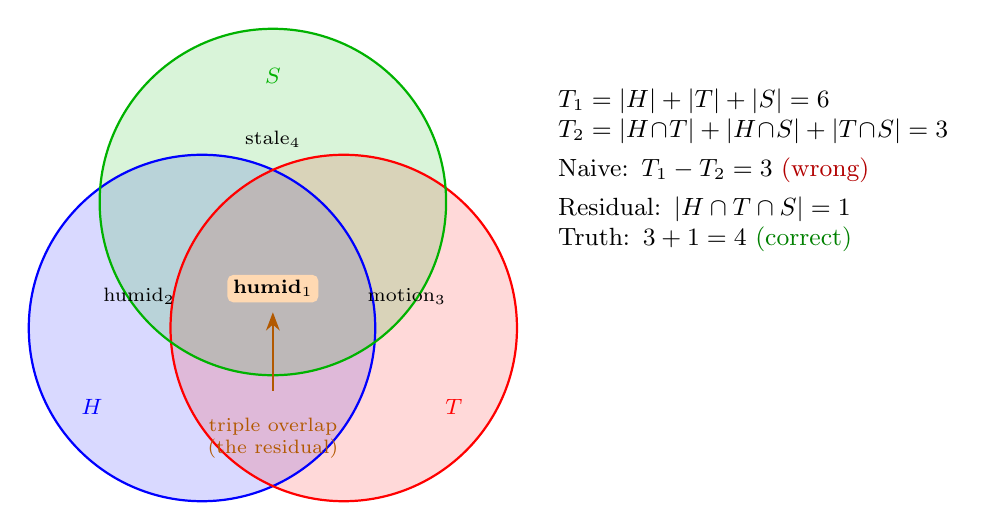
\begin{tikzpicture}[
  >=Stealth,
  every node/.style={font=\footnotesize},
]
% Three overlapping circles
\begin{scope}[opacity=0.15]
  \fill[blue] (0, 0) circle (22mm);
  \fill[red] (18mm, 0) circle (22mm);
  \fill[green!70!black] (9mm, 16mm) circle (22mm);
\end{scope}
\draw[blue, thick] (0, 0) circle (22mm);
\draw[red, thick] (18mm, 0) circle (22mm);
\draw[green!70!black, thick] (9mm, 16mm) circle (22mm);

% Labels
\node[blue, font=\footnotesize\bfseries] at (-14mm, -10mm) {$H$};
\node[red, font=\footnotesize\bfseries] at (32mm, -10mm) {$T$};
\node[green!70!black, font=\footnotesize\bfseries] at (9mm, 32mm) {$S$};

% Unique elements
\node at (-8mm, 4mm) {\scriptsize humid$_2$};
\node at (26mm, 4mm) {\scriptsize motion$_3$};
\node at (9mm, 24mm) {\scriptsize stale$_4$};

% Triple overlap (center)
\node[fill=orange!30, rounded corners=2pt, inner sep=2pt,
      font=\scriptsize\bfseries] at (9mm, 5mm) {humid$_1$};

% Annotation
\draw[->, thick, orange!70!black] (9mm, -8mm) -- (9mm, 2mm);
\node[font=\scriptsize, text=orange!70!black, text width=30mm,
      align=center] at (9mm, -14mm)
  {triple overlap\\(the residual)};

% Right side: computation
\node[anchor=west, font=\small, text width=52mm] at (44mm, 20mm) {
  $T_1 = |H| + |T| + |S| = 6$\\
  $T_2 = |H\!\cap\! T| + |H\!\cap\! S| + |T\!\cap\! S| = 3$\\[3pt]
  Naive: $T_1 - T_2 = 3$ \textcolor{red!70!black}{(wrong)}\\[3pt]
  Residual: $|H \cap T \cap S| = 1$\\
  Truth: $3 + 1 = 4$ \textcolor{green!50!black}{(correct)}
};
\end{tikzpicture}
\caption{The inclusion-exclusion gap in Maple Court.  Three inference
rules share the humid$_1$ reading (orange center).  Pairwise
overlaps are visible, but the triple overlap---the residual---is
what the two-term estimate misses.}
\label{fig:multideduction-venn}
\end{figure}

\noindent
The diagram makes the geometry clear: the orange center (triple
overlap) is subtracted once too many by the two-term formula.
The full inclusion-exclusion adds it back:
\[
  |H \cup T \cup S| = \underbrace{|H| + |T| + |S|}_{T_1 = 6}
  - \underbrace{|H \!\cap\! T| + |H \!\cap\! S| + |T \!\cap\! S|}_{T_2 = 3}
  + \underbrace{|H \cap T \cap S|}_{\text{residual} = 1}
  = 4
\]
Theorem~\ref{thm:ie-no-go} says that no function
of $(T_1, T_2)$ alone can recover the~4: a \emph{different}
configuration with the same $(T_1, T_2) = (6, 3)$ has union
cardinality~3 (no triple overlap).  The two are indistinguishable
from pairwise statistics---a classical fact, but one that bites
concretely in multi-rule PLN inference.

\paragraph{Practical consequences.}
For a PLN system running $k$ inference rules that may share evidence:
\begin{itemize}
\item If the rules' evidence sets form a \emph{tree} (each
  observation appears in at most two rules), the triple overlap is
  zero and the two-term estimate is exact.
\item If the evidence graph has cycles (an observation feeds three or
  more rules), the residual is nonzero and the system must either
  compute it or accept the undercount.
\item The residual decomposition
  (Theorem~\ref{thm:residual-decomp}) gives the exact correction
  when the triple overlap is known or bounded.
\item When the residual is unknown but pairwise statistics are
  available, classical bounds (Hunter~\cite{Hunter1976},
  Kounias--Sotirakoglou~\cite{KouniasSotirakoglou1989}) or
  LP-based sharp bounds (Pr\'ekopa~\cite{Prekopa1988}) provide
  principled alternatives to PLN's empirical $\xi$~correction.
  Formalizing these bounds in the WM setting is an open target.
\item The practical question is often not ``is the combined
  probability exact?''\ but ``does the approximate combination
  select the right inference path?''\ --- the same distinction
  that makes naive Bayes effective for classification despite
  violated independence
  assumptions~\cite{DomingosPazzani1997, Zhang2004NaiveBayes}.
  The WM contribution is to make this tradeoff explicit
  via typed guard conditions rather than leaving it implicit.
\end{itemize}

\noindent
In operational terms, the guarded contract for multideduction is:
\begin{enumerate}
\item If the residual is known or structurally zero (tree BN),
  use the corrected multideduction rewrite---it is exact.
\item If only pairwise data is available, use a bound-carrying
  rule (Hunter/Kounias/Pr\'ekopa) and propagate the interval.
\item Otherwise, mark the result as heuristic or escalate to
  an exact WM/BN query.
\end{enumerate}


\section{Trail-Free Protocol Dynamics}
\label{sec:trail-free}

A trail-free protocol re-derives conclusions from scratch at each
step, without recording which evidence has already been processed.
This is the simplest operational strategy---and it can fail to
converge.

\begin{theorem}[Trail-free non-stabilization (\claimBoundary{})]
\label{thm:trail-free-no-go}
There exists a two-state system where the trail-free deterministic
update enters a period-2 cycle and never reaches a fixed point.%
\footnote{Formalized:
\code{orbit\_not\_eventually\_constant}
in \codepath{Mettapedia/Logic/PLNTrailFreeDynamicsCounterexample.lean}
  The counterexample is a single toggle function on
\code{Bool} with no fixed point.}
\end{theorem}

\noindent
The counterexample is minimal: a protocol step that toggles the
truth value.  On every even step the state is \code{true}; on every
odd step, \code{false}.  The orbit has period~2 and no fixed point
exists (proved: \code{trailFreeStep\_ne\_self}).  Without a trail, the
protocol re-processes the same evidence in opposite order on each
step.

The positive result under fresh evidence:

\begin{theorem}[Damped convergence (\claimConditional{})]
\label{thm:damped-convergence}
If fresh evidence is eventually available (there exists $N$ such
that $\mathrm{freshAt}(n) = \mathrm{true}$ for all $n \ge N$),
then the damped SP/SPN protocol stabilizes: all states from step
$N+1$ onward equal the fresh-evidence state.

Under bounded-gap fairness (every window of $B$ steps contains at
least one fresh tick), the inconsistency metric hits zero within
$B + 1$ steps of any point.%
\footnote{Formalized:
\code{damped\_sp\_spn\_eventually\_constant\_of\_eventual\_fresh}
and \code{inconsistency\_zero\_within\_bound\_of\_boundedGapFresh}
in \codepath{Mettapedia/Logic/PLNTrailFreeDampedConvergence.lean}
}
\end{theorem}

\noindent
This pair of theorems shows the sharp boundary: trail-free without
fresh evidence can diverge; trail-free with eventual fresh evidence
always converges.  Fresh-evidence injection breaks the cycle: when
a new observation arrives, it overwrites the oscillating state,
anchoring the orbit to the fresh-evidence value.  Without fresh
evidence, the same toggling dynamics replay indefinitely.

\begin{figure}[htbp]
\centering
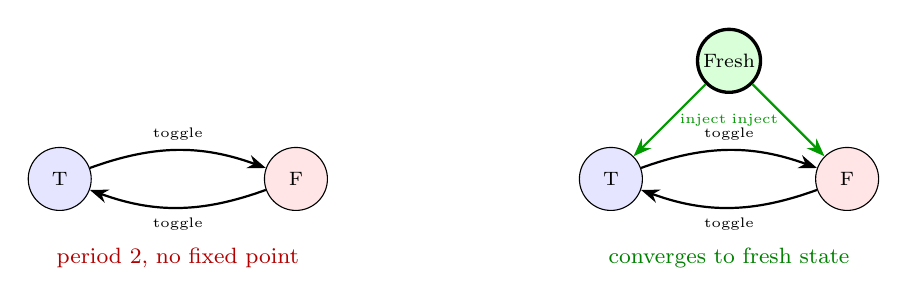
\begin{tikzpicture}[
  >=Stealth, every node/.style={font=\scriptsize},
  state/.style={draw, circle, minimum size=8mm, inner sep=1pt},
]
\node[state, fill=blue!10] (T) at (0, 0) {T};
\node[state, fill=red!10] (F) at (3, 0) {F};
\draw[->, thick, bend left=20] (T) to
  node[above, font=\tiny] {toggle} (F);
\draw[->, thick, bend left=20] (F) to
  node[below, font=\tiny] {toggle} (T);
\node[font=\footnotesize, text=red!70!black] at (1.5, -1)
  {period 2, no fixed point};

\node[state, fill=blue!10] (T2) at (7, 0) {T};
\node[state, fill=red!10] (F2) at (10, 0) {F};
\node[state, fill=green!15, very thick] (Fr) at (8.5, 1.5)
  {Fresh};
\draw[->, thick, bend left=20] (T2) to
  node[above, font=\tiny] {toggle} (F2);
\draw[->, thick, bend left=20] (F2) to
  node[below, font=\tiny] {toggle} (T2);
\draw[->, thick, green!60!black] (Fr) to
  node[right, font=\tiny] {inject} (T2);
\draw[->, thick, green!60!black] (Fr) to
  node[left, font=\tiny] {inject} (F2);
\node[font=\footnotesize, text=green!50!black] at (8.5, -1)
  {converges to fresh state};
\end{tikzpicture}
\caption{Trail-free dynamics: without fresh evidence (left), the
protocol oscillates.  With fresh evidence injection (right), it
converges.}
\label{fig:trail-free-dynamics}
\end{figure}


\section{Pooling and Fusion}
\label{sec:pooling}

When multiple agents or multiple inference paths produce evidence
for the same query, the system must \emph{pool} their outputs.
The formalization captures this via a \code{PoolingOperator}
structure with four axioms:
\begin{enumerate}
\item Commutativity: $\mathrm{pool}(s_1, s_2) = \mathrm{pool}(s_2, s_1)$.
\item Associativity: pooling is independent of grouping.
\item Two-sided neutrality: pooling with the zero scorer is the
  identity.
\item External Bayesianity:
  $\mathrm{pool}(\mathrm{update}(s_1, \ell),\;
  \mathrm{update}(s_2, \ell)) =
  \mathrm{update}(\mathrm{pool}(s_1, s_2),\; \ell)$.
\end{enumerate}

\noindent
One might hope these axioms pin down additive fusion.  They do not.

\begin{theorem}[Pooling non-uniqueness (\claimBoundary{})]
\label{thm:pooling-non-unique}
The max-pooling operator
$\mathrm{pool}(e_1, e_2) = (\max(n_1^+, n_2^+),\; \max(n_1^-, n_2^-))$
satisfies all four axioms---including external
Bayesianity---yet differs from additive fusion.%
\footnote{Formalized:
\code{maxPoolingOperator} (satisfies all fields of
\code{PoolingOperator}) and
\code{maxPoolingOperator\_ne\_fuse} in
\codepath{Mettapedia/Logic/PremiseSelectionExternalBayesianity.lean}
}
\end{theorem}

\noindent
The reason: max distributes over coordinatewise multiplication
(the update operation), so external Bayesianity holds.  But max is
not \emph{additive on totals}: $\max(3, 2) \ne 3 + 2$.  The
additional constraint that recovers uniqueness is
\emph{total additivity}:
$\mathrm{pool}(x, y).\mathrm{total} =
x.\mathrm{total} + y.\mathrm{total}$.
This is a natural requirement: pooling two independent evidence
bodies should give a total observation count equal to the sum of
their individual counts.

\begin{theorem}[Pooling uniqueness under total additivity
  (\claimConditional{})]
\label{thm:pooling-unique}
External Bayesianity plus total additivity uniquely recovers
additive evidence pooling: for all $x, y$,
$\mathrm{pool}(x, y) = x + y$.%
\footnote{Formalized:
\code{poolE\_eq\_hplus\_of\_externalBayes\_totalAdd} and
\code{poolingOperator\_pointwise\_unique\_of\_externalBayes\_totalAdd}
in the same file.  The proof uses mask projections to decompose
into positive and negative components.}
\end{theorem}

\maplecourt{%
Maple Court's three WM layers instantiate evidence pooling
concretely.  Each apartment exports evidence summaries---not raw
sensor traces---to the building WM, which pools them via additive
fusion.  The pooling-uniqueness theorem justifies this: under
external Bayesianity and total additivity, additive pooling is the
unique fusion rule.  At the \emph{community scale}, multiple
buildings export building-level summaries to a shared district WM.
The privacy export theorem guarantees that the community WM cannot
reconstruct apartment-level occupancy from the aggregated summaries.}


\section{Order-Cost Governance}
\label{sec:order-cost}

When revision is not purely commutative---or when an operational
schedule reorders evidence arrival---the system needs bounds on the
resulting error.  The order-cost framework quantifies this.  This is
the formal content behind axis~9 (Cost) of the 13-axis vertex family
(Chapter~\ref{ch:typed}, \S\ref{sec:wm-13axis}): enabling cost
tracking at a vertex adds these order-cost rules to the calculus.

\begin{definition}[Swap anomaly]
The swap anomaly count for states $W_1, W_2$ at query~$q$ under
an overlap layer~$L$ is
\[
  \mathrm{SwapAnomaly}_L(W_1, W_2, q) :=
  |\mathrm{obsCount}(L.\mathrm{merge}(W_1, W_2), q) -
   \mathrm{obsCount}(L.\mathrm{merge}(W_2, W_1), q)|
\]
the symmetric count-level discrepancy when the merge order is
swapped.
\end{definition}

\begin{theorem}[Order-cost budget bound (\claimConditional{})]
\label{thm:order-cost}
If each adjacent swap in a schedule is bounded by a per-step budget,
the total schedule error is bounded by the sum of those budgets.
Commutative merge-evidence implies zero swap anomaly and zero
schedule error.%
\footnote{Formalized:
\code{scheduleErrorBound\_of\_pairwise\_bounds} and
\code{swapAnomalyCount\_zero\_of\_commutativeMergeEvidence}
in \codepath{Mettapedia/Logic/PLNWorldModelOrderCostBounds.lean}
}
\end{theorem}

\begin{theorem}[Runtime audit certificate soundness (\claimConditional{})]
\label{thm:audit-cert}
If runtime pairwise-order checks pass with budget vector~$B$, then
the formal schedule-error bound and budget-threshold policy
conclusions follow.  A single swap-step check certifies the
two-step policy threshold.%
\footnote{Formalized:
\code{runtimePairwiseOrderCheck\_certifies\_scheduleErrorBound}
in \codepath{Mettapedia/Logic/PLNWorldModelOrderCostAuditCertificate.lean}
}
\end{theorem}

\noindent
Concrete demos prove that (a)~weighted numeric merge has nontrivial
non-commutative behavior, and (b)~batch swap under additive merge
has certified zero order-cost.%
\footnote{Formalized in
\codepath{Mettapedia/Logic/PLNWorldModelOrderCostWeightedDemo.lean} and
\codepath{Mettapedia/Logic/PLNWorldModelOrderCostGasPolicyDemo.lean}.}
A provenance-tracked variant using the \code{Which} semiring
demonstrates that right-biased (latest-wins) merge on
provenance-tracked states has maximum swap anomaly ($\top$)
when one state is zero and the other is nonzero---the
provenance structure makes order effects maximally visible.%
\footnote{Formalized in
\codepath{Mettapedia/Logic/PLNWorldModelOrderCostProvenanceDemo.lean}
(5~theorems, 0~sorry).}


\section{Stochastic Experiment and Blackwell Factorization}

When choosing \emph{which experiment to run next} (which sensor to
query, which feature to observe), the value of an experiment is
determined by the Blackwell factorization:

\begin{itemize}
\item Expected utility equals the Blackwell factor.
\item Optimal value is monotone under Blackwell domination: a more
  informative experiment is always at least as valuable.
\item Trusted-gate transfer preserves the optimality ordering.
\end{itemize}

\noindent
This connects the WM calculus to the theory of statistical
experiments (Blackwell 1953, Le Cam 1964): the value-of-information
computation is a world-model query about the expected gain from
evidence not yet observed.%
\footnote{Formalized in
\codepath{Mettapedia/Logic/PLNWorldModelExperimentStochastic.lean}
}


%% ═══════════════════════════════════════════════════════
%% PART 2: INFERENCE CONTROL
%% ═══════════════════════════════════════════════════════

\section{Selector Specifications}
\label{sec:selectors}

A \emph{selector} chooses which premises to use for the next
inference step.  The formalization provides typed selector
specifications with two robustness properties:

\begin{description}
\item[Ranking transfer.] If a selector produces a good ranking on
  one distribution, it produces a good ranking on similar
  distributions.
\item[Ranking stability.] Small perturbations in the knowledge base
  produce small perturbations in the ranking.
\end{description}

\noindent
These ensure that a selector trained on one corpus does not
catastrophically fail when deployed on a slightly different one---a
concern entirely absent from the original PLN book but pressing in
any practical system.%
\footnote{Formalized in
\codepath{Mettapedia/Logic/PremiseSelectionSelectorSpec.lean}
 and
\codepath{Mettapedia/Logic/PremiseSelectionRankingStability.lean}
}

\paragraph{Demand-directed backward chaining.}
An orthogonal approach to premise selection: instead of scoring
premises by relevance, propagate \emph{demand} backward from the
query through the factor graph.  Each premise receives a demand
score proportional to its information need (how uncertain it is)
and its sensitivity (how much the query answer depends on it).
The unknown intermediate Dog(Lassie) in a chain
Collie $\to$ Dog $\to$ Mammal gets demand $1000$ (maximum: both
maximally uncertain and maximally sensitive), while the well-known
Collie gets demand~$50$.  After forward supply fills Dog's
confidence, demand \emph{contracts} from $1000$ to $240$
(Proposition~2 of~\cite{Goertzel2026BackwardChaining}).
Forgetting an observation reopens demand at the affected
premise---the same \code{forget} pattern used throughout the
evidence algebra.%
\footnote{Formalized in
\codepath{Mettapedia/Logic/WMDemandDemo.lean}
(258~lines, 27~theorems, 0~sorry).  The demo kernel-checks
forward supply, information need, sensitivity, demand ordering
$(1000 > 210 > 191 > 50)$, demand contraction after supply, and
demand reopening after forgetting.}
On a fork+chain topology with a hidden common cause
($A \leftarrow H \to B \to C \to D$), the same framework
exercises multi-path demand aggregation: when the fork arm~$A$ is
observed, the chain path carries all the demand; forgetting~$A$
activates the fork arm and rebalances demand across both paths.%
\footnote{Formalized in
\codepath{Mettapedia/Logic/WMForkDemandDemo.lean}
(23~theorems, 0~sorry).}


\section{Coverage and Submodularity}
\label{sec:coverage}

Let $D$ be the set of true dependencies and $S$ the selected premise
set.  The coverage objective is $f(S) = |S \cap D|$.

\begin{theorem}[Coverage submodularity (\claimCore{})]
\label{thm:coverage-submod}
The function $f$ is monotone ($S \subseteq T \Rightarrow f(S) \le f(T)$)
and submodular: for $S \subseteq T$ and any element $x \notin T$:
\[
  f(T \cup \{x\}) - f(T) \;\le\; f(S \cup \{x\}) - f(S).
\]
\end{theorem}

\noindent
By the classical result of Nemhauser, Wolsey, and Fisher, the greedy
algorithm (iteratively adding the element with maximum marginal gain)
achieves a $(1 - 1/e) \approx 0.632$ approximation ratio for monotone
submodular maximization under cardinality constraints.  The guarantee
is formalized via an explicit \code{GreedyChain} inductive
construction.%
\footnote{Formalized:
\code{dependencyCoverage\_mono},
\code{dependencyCoverage\_insert} (diminishing returns),
and \code{GreedyChain} in
\codepath{Mettapedia/Logic/PremiseSelectionCoverage.lean}
}

\maplecourt{%
The hallway cleaning robot must decide which floor to clean first,
given limited battery.  It queries the building WM for humidity and
laundry traffic on each floor.  The greedy coverage selector picks
the floor with maximum marginal information gain.  A
$\Sigma$-guarded rewrite infers ``hallway needs cleaning'' from the
humidity and traffic evidence, firing only when d-sep conditions are
met.  The $(1 - 1/e)$ coverage bound guarantees that the robot's
greedy floor-selection is near-optimal.}


\section{Coverage Surrogate Boundaries}
\label{sec:surrogate-nogo}

A natural simplification: replace the joint coverage function with
a per-premise score (each premise's individual relevance) and optimize
the surrogate.  This is impossible in general.

\boundarystart
\begin{theorem}[Coverage/cardinality surrogate no-go (\claimBoundary{})]
\label{thm:surrogate-no-go}
Coverage and cardinality together are insufficient for risk-sensitive
selection.  There exist premise sets with identical coverage and
cardinality but different false-positive risk.%
\footnote{Formalized:
\codepath{Mettapedia/Logic/PremiseSelectionCoverageCounterexamples.lean}
}
\end{theorem}
\boundaryend

\noindent
The counterexample constructs two premise sets that look identical to
any local surrogate (same size, same coverage count) but differ in
\emph{which} dependencies they hit.  One set covers high-risk
dependencies; the other covers low-risk ones.  The greedy algorithm
must evaluate the actual joint coverage function at each step, not a
decomposable proxy.


\section{BRGI and Feasible Sets}

The Balanced Relevance-Guided Inference (BRGI) framework provides an
optimization-theoretic perspective on inference scheduling:
\begin{itemize}
\item Finite feasible sets with policy-sensitive optimum
  characterization.
\item Graph-level BRGI objects with optimality-preserving refinement.
\end{itemize}

\noindent
BRGI connects the WM calculus to the combinatorial optimization
literature: the inference-control problem is a submodular optimization
problem on a graph of possible inference steps.%
\footnote{Formalized in
\codepath{Mettapedia/Logic/PremiseSelectionBRGI.lean}}


\section{The Composed End-to-End Pipeline}
\label{sec:composed-pipeline}

The final result composes the entire pipeline into a single
correctness theorem: selector $\to$ rewrite $\to$ threshold.

\begin{theorem}[End-to-end pipeline correctness (\claimConditional{})]
\label{thm:end-to-end}
Given a selector that produces a ranked premise set, a compiled
rewrite that applies a PLN rule under BN side conditions, and a
threshold that accepts the result, the composed pipeline is correct:
if the selector has sufficient coverage and the side conditions are
met, the accepted result agrees with the full posterior query up to
the distributional approximation bound of
Chapter~\ref{ch:error-transport}.%
\footnote{Formalized:
\code{ch9\_selector\_rewrite\_threshold\_end\_to\_end\_of\_interval}
in \codepath{Mettapedia/Logic/PLNCanonicalAPI.lean}}
\end{theorem}

\begin{figure}[htbp]
\makebox[\textwidth][c]{%
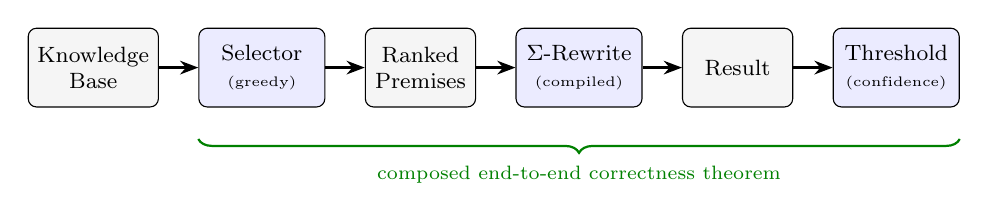
\begin{tikzpicture}[
  >=Stealth,
  every node/.style={font=\footnotesize},
  box/.style={draw, rounded corners=3pt, align=center,
              minimum height=10mm},
  stage/.style={box, fill=blue!8, minimum width=16mm},
  data/.style={box, fill=gray!8, minimum width=14mm},
]
\node[data] (kb) {Knowledge\\Base};
\node[stage, right=5mm of kb] (sel) {Selector\\{\tiny(greedy)}};
\node[data, right=5mm of sel] (prem) {Ranked\\Premises};
\node[stage, right=5mm of prem] (rew) {$\Sigma$-Rewrite\\{\tiny(compiled)}};
\node[data, right=5mm of rew] (res) {Result};
\node[stage, right=5mm of res] (thr) {Threshold\\{\tiny(confidence)}};

\draw[->, thick] (kb) -- (sel);
\draw[->, thick] (sel) -- (prem);
\draw[->, thick] (prem) -- (rew);
\draw[->, thick] (rew) -- (res);
\draw[->, thick] (res) -- (thr);

\draw[decorate, decoration={brace, amplitude=5pt, mirror},
      thick, green!50!black]
  ($(sel.south west) + (0, -4mm)$) --
  node[below=6pt, font=\scriptsize, green!50!black]
    {composed end-to-end correctness theorem}
  ($(thr.south east) + (0, -4mm)$);
\end{tikzpicture}}
\caption{The inference-control pipeline.  A selector chooses premises;
a $\Sigma$-guarded compiled rewrite produces a result; a threshold
accepts or rejects.  The composed pipeline has a single end-to-end
correctness theorem.}
\label{fig:inference-control-pipeline}
\end{figure}

\noindent
This is the technical endpoint of the entire compiled-inference story.
The calculus begins with a correct kernel (Part~II), develops exact
shortcuts under side conditions (Chapters~\ref{ch:sigma-rewrites}--\ref{ch:bn-models}), quantifies the cost of approximation
(Chapter~\ref{ch:error-transport}), and now composes
selection, execution, and acceptance into a single
pipeline with a single correctness proof.

The pipeline diagram (Figure~\ref{fig:inference-control-pipeline})
should be read right-to-left as a specification:
\emph{what does the system guarantee?}  And left-to-right as an
implementation: \emph{how does the system compute?}  Both readings
are justified by the same theorem.


\section{Connections to Automated Theorem Proving}
\label{sec:atp}

The coverage objective $f(S) = |S \cap D|$ and the greedy
$(1 - 1/e)$ approximation are not specific to PLN.  They are the
same structures that arise in \emph{premise selection} for
interactive and automated theorem provers---the problem of choosing
which library lemmas to feed to a prover given a goal.

The connection is exact.  The MaSh (Machine-learning for Sledgehammer)
framework uses $k$-nearest-neighbor and naive-Bayes classifiers to
rank premises.  Both are world-model instances
(Chapter~\ref{ch:bn-models}, \S\ref{sec:bridge-nb-knn}): Naive Bayes
is a BN fork, $k$-NN is evidence-weighted revision from the $k$
nearest neighbors.  The formalization makes this explicit: a
$k$-NN premise selector IS an additive world-model query, and the
coverage bound applies to it.%
\footnote{Formalized in
\codepath{Mettapedia/Logic/PremiseSelectionKNN.lean} and
\codepath{Mettapedia/Logic/PremiseSelectionKNN\_PLNBridge.lean}.}

Three questions that this bridge raises for the ATP community:

\begin{enumerate}
\item \textbf{Completeness under budget.}  The $(1 - 1/e)$ bound
  guarantees near-optimal coverage for a fixed cardinality budget~$k$.
  But ATP premise selection operates under iterative deepening:
  if the first $k$ premises fail, the prover tries $2k$, then $4k$.
  Does the formal coverage bound compose across rounds?  The
  submodularity of $f$ ensures diminishing returns, but the
  interaction with prover timeouts is not yet formalized.

\item \textbf{Learned approximations.}  The formal bound assumes
  access to the oracle gain function $\mathrm{dependencyGain}(D, S, a)$.
  A learned selector (neural, $k$-NN, gradient-boosted) approximates
  this gain.  The ranking-stability theorem
  (\S\ref{sec:selectors}) bounds the degradation under
  small perturbations, but characterizing the full approximation gap
  for specific learners is open.

\item \textbf{Runtime cost.}  Evaluating $\mathrm{dependencyGain}$
  at each greedy step costs $O(|D|)$ per candidate.  For a library
  of $10^5$ premises and a budget of $k = 500$, the greedy chain
  requires $\sim 5 \times 10^7$ gain evaluations.  Approximate
  gain via cached features reduces this to $O(k \cdot |D|)$ with a
  constant-factor overhead from feature extraction.
\end{enumerate}

\noindent
These connections are not speculative: the project includes
experimental evaluation of PLN-based premise selectors against MaSh
baselines on the extended MPTP~2078 benchmark (5,049~problems), with results
competitive with $k$-NN at lower premise counts.%
\footnote{See the \codepath{atps/} directory for scripts,
datasets, and evaluation results.}


%% ═══════════════════════════════════════════════════════════════════
\part{Additional Semantic Families}
\label{part:families}
%% ═══════════════════════════════════════════════════════════════════

\chapter{Intensional Inheritance}
\label{ch:intensional}

Two concepts $A$ and $B$ may be related in two ways.
\emph{Extensional} inheritance measures overlap of instances:
$P(B \mid A) = n_{AB}^+ / n_A$.  \emph{Intensional} inheritance
measures shared properties: how much does knowing $A$'s property
profile tell you about $B$?  Classical PLN treats these as separate
channels with a scalar mixing parameter.  The formalization shows
that this is both less and more than what the mathematics supports:
the scalar mixture is refuted, but a clean information-theoretic
unification replaces it.  The result connects to the evidence
carriers of Chapter~\ref{ch:evidence} and the typed world-model
grounding of Chapter~\ref{ch:typed}.


\section{The Information-Theoretic Unification}

Goertzel (2025) gives the unifying formula:
\[
  P(W \mid F) = P(W) \cdot 2^{I(F;\,W)}
\]
where $I(F; W) = \sum_{f,w} p(f,w) \log_2 \frac{p(f,w)}{p(f) \cdot
p(w)}$ is the Shannon mutual information between the feature profile
$F$ and the target concept~$W$.  Extensional inheritance is the left
side; intensional inheritance is the exponent on the right.%
\footnote{Formalized:
\code{goertzel\_formula} in
\codepath{Mettapedia/Logic/IntensionalInheritance.lean}
}

\begin{theorem}[Singleton reduction (\claimCore{})]
\label{thm:singleton-reduction}
When every property is a singleton (each property picks out exactly
one element), the mutual information $I(F; W)$ equals
$\log_2(P(W \mid F) / P(W))$, and the Goertzel formula reduces to
the tautology $P(W \mid F) = P(W \mid F)$.  Intensional inheritance
collapses to extensional inheritance when concepts have no internal
structure.%
\footnote{Formalized: \code{singleton\_reduction} in the same file.}
\end{theorem}

\noindent
The philosophical point (Goertzel): ``creatures with hearts'' and
``creatures with kidneys'' seem like different concepts (different
intensions), but they pick out the same class (same extension)
because hearts and kidneys co-evolved.  The information-theoretic
view captures this: $I(\text{heart}; \text{kidney}) \approx 1$.

\maplecourt{%
In Maple Court, apartments share structural properties: kitchens,
bathrooms, plumbing risers, the same building infrastructure.
Intensional similarity between Apartment~3B and Apartment~5C is
high---their property profiles overlap almost completely (both are
west-facing corner units with similar heat and humidity patterns).
But extensional inheritance diverges: Apartment~3B has a pipe leak
while 5C does not.  The typed WM grounding resolves this: extensional
queries use per-apartment evidence, while intensional queries
aggregate over shared property patterns via the ASSOC channel.}


\section{Typed WM Grounding}

The WM approach grounds intensional inheritance via a typed query
family:

\begin{definition}[Inheritance sort]
\[
  \mathrm{InheritanceSort} \;=\;
  \mathrm{extensional} \;\mid\;
  \mathrm{intensionalAssoc} \;\mid\;
  \mathrm{intensionalPAT} \;\mid\;
  \mathrm{mixed}
\]
Each sort has its own evidence extraction and strength computation.%
\footnote{Formalized in
\codepath{Mettapedia/Logic/PLNIntensionalWorldModel.lean}
}
\end{definition}

\noindent
The ASSOC channel computes association strength via mutual
information: $P_{\mathrm{ASSOC}}(W \mid F) = P(W) \cdot 2^{I(F; W)}$.
High ASSOC inheritance means knowing which properties $A$ has gives
strong predictive power for which properties $B$ has.  The PAT
channel provides a complementary structural route based on
property-pattern proximity beyond what mutual-information association
captures.


\section{Solomonoff Bridge}

The Solomonoff bridge connects intensional inheritance to algorithmic
information theory via the universal-mixture log-ratio:
\[
  I_{\mathrm{int},\xi}(W, F, x) =
  \log_2 \frac{P_\xi(W \mid F, x)}{P_\xi(W \mid x)}
\]
when both conditionals are positive.  Specialized
\code{xiSemimeasure} and geometric-mixture versions are proved as
explicit theorem endpoints.%
\footnote{Formalized:
\code{intensionalFromConditional\_eq\_log2\_ratio} and
\code{intensionalFromXiGeom\_eq\_log2\_ratio} in
\codepath{Mettapedia/Logic/IntensionalInheritanceSolomonoffBridge.lean}
}


\section{Mixed Semantic Packaging}

The original PLN book proposes a simple scalar mixture:
$\mathrm{InhInt}(A, B) = \alpha \cdot \mathrm{Ext}(A, B)
+ (1 - \alpha) \cdot \mathrm{IntAssoc}(A, B)$.  The formalization
explicitly refutes this:

\begin{theorem}[No binary mixed policy (\claimBoundary{})]
\label{thm:no-mixed-policy}
There exists a concrete state with evidence scores $(3, 2, 1)$ for
(extensional, ASSOC, PAT) channels such that the PAT channel
contributes nontrivially and the mixed result cannot be expressed
as any function of only the extensional and ASSOC values.%
\footnote{Formalized in
\codepath{Mettapedia/Logic/PLNIntensionalCanary.lean}
}
\end{theorem}

\noindent
The book's binary mixture is not merely incomplete but false as a
general law: the full three-channel model (extensional, ASSOC, PAT)
is needed.  The corrected surface is a typed three-channel mixed
rule with selector-specialized endpoints.%
\footnote{Formalized in
\codepath{Mettapedia/Logic/PLNIntensionalAssocPatClosure.lean}
}

\medskip\noindent
Intensional inheritance is the first semantic family that extends
the query language rather than the state or the carrier.  The
same state and the same evidence algebra serve both extensional and
intensional queries; only the \code{InheritanceSort} index
changes.  This pattern---extending the calculus by enriching the
query type---recurs in the temporal and normative families that
follow.


%% ─────────────────────────────────────────────────────────────────

\chapter{Temporal and Causal Inference}
\label{ch:temporal}

The world-model calculus so far is atemporal: the state records
evidence about the world \emph{now}.  This chapter extends the
framework to time-indexed states and temporal queries, and shows
that the extension has a clean algebraic structure---the temporal
quantale---that yields temporal transitivity as a free theorem.


\section{Temporal Operators}

Temporal predicates live in the type
$\mathrm{TemporalPred}(D, T) = D \to T \to \mathrm{Prop}$,
where $D$ is the domain and $T$ is the time type.  Three layers of
operators build the temporal algebra:

\begin{definition}[Simultaneous operators (\claimCore{})]
\begin{align*}
  \mathrm{SimAND}(P, Q)(x, t) &:= P(x, t) \wedge Q(x, t) \\
  \mathrm{SimOR}(P, Q)(x, t)  &:= P(x, t) \vee Q(x, t)
\end{align*}
Both predicates hold (or at least one holds) at the same moment.
\end{definition}

\begin{definition}[Sequential operators (\claimCore{})]
\begin{align*}
  \mathrm{SeqAND}(P, Q)(x, t) &:= P(x, t) \;\wedge\;
    \exists \Delta > 0.\; Q(x, t + \Delta) \\
  \mathrm{SeqAND}_f(P, Q)(x, t) &:= P(x, t) \;\wedge\;
    \exists \Delta.\; f(\Delta) \wedge Q(x, t + \Delta)
\end{align*}
where $f$ constrains the delay (e.g., $\Delta \in [1, T_{\max}]$).
\end{definition}

\begin{definition}[Predictive implication (\claimCore{})]
\[
  \mathrm{PredImpl}(P, Q)(x, t) := P(x, t) \;\Rightarrow\;
  \exists \Delta > 0.\; Q(x, t + \Delta)
\]
The 3-node predictive chain composes:
\[
  \mathrm{PredChain}_3(T_1, T_2, A, B, C) :=
  \mathrm{SeqAND}_{T_1}\!\bigl(A,\;
    \mathrm{SeqAND}_{T_2}(B, C)\bigr).
\]%
\footnote{Formalized in
\codepath{Mettapedia/Logic/PLNTemporalCausalInference.lean}
}
\end{definition}


\section{The Temporal Quantale}

The Boolean skeleton above lifts to a quantale-valued setting with
a clean algebraic structure.

\begin{definition}[Temporal quantale (\claimCore{})]
A temporal quantale is a commutative quantale $Q$ equipped with a
group action $\varphi : T \to (Q \to Q)$ by quantale automorphisms:
\begin{itemize}
\item $\varphi_0 = \mathrm{id}$, \quad
  $\varphi_{t+t'} = \varphi_t \circ \varphi_{t'}$
\item Each $\varphi_t$ preserves $*$, $\bot$, $\top$, and $\bigsqcup$
\item Since $T$ is a group, $\varphi_t$ is invertible
  ($\varphi_{-t}$ is the inverse), hence an automorphism
\end{itemize}%
\footnote{Formalized:
\code{TemporalQuantale} class in
\codepath{Mettapedia/Logic/TemporalQuantale.lean}}
\end{definition}

\noindent
The key payoff: automorphisms preserve the product and the lattice
order, so they preserve residuation (implication), which is definable
from both.  Temporal transitivity is therefore a \emph{free
theorem}---no additional axioms are needed:

\begin{theorem}[Temporal transitivity (\claimCore{})]
\label{thm:temporal-transitivity}
For any $a, b, c \in Q$ and time offsets $t_1, t_2 \in T$:
\[
  (a \Rightarrow \varphi_{t_1} b) \;*\;
  \varphi_{t_1}(b \Rightarrow \varphi_{t_2} c)
  \;\le\;
  (a \Rightarrow \varphi_{t_1 + t_2} c)
\]
Temporal modus ponens is the special case $c = \top$:
$a \;*\; (a \Rightarrow \varphi_t b) \;\le\; \varphi_t b$.%
\footnote{Formalized:
\code{temporal\_transitivity} and
\code{temporal\_modus\_ponens} in the same file.}
\end{theorem}

\noindent
In PLN terms: $Q$ represents evidence values, $*$ is conjunction
under independence, $\Rightarrow$ is implication strength, and
$\varphi_t$ shifts evidence across time.  The theorem says chained
temporal implications compose without loss of algebraic structure.


\section{Causal Profile and Event Calculus}

Causal inference is grounded through a probabilistic event calculus
built on four predicates: $\mathrm{Happens}(e, t)$,
$\mathrm{Initiates}(e, f, t)$, $\mathrm{Terminates}(e, f, t)$, and
$\mathrm{HoldsAt}(f, t)$.  For a pair of predicates $(A, B)$, the
\emph{causal profile} collects predictive implication strengths across
temporal lags:
\[
  \mathrm{CausalProfile}(A, B) =
  \bigl\{\mathrm{strength}(\mathrm{PredImpl}_\Delta(A, B))
  \;\mid\; \Delta \in [1, T_{\max}]\bigr\}
\]%
\footnote{Formalized in
\codepath{Mettapedia/Logic/PLNTemporalCausalInference.lean} and
\codepath{Mettapedia/Logic/PLNProbabilisticEventCalculus.lean}
}


\section{Distinguishing Cause from Correlation}

A high predictive-implication strength does not by itself establish
causation.  The formalization introduces a precise discriminator
using the intensional/extensional distinction from
Chapter~\ref{ch:intensional}:

\begin{definition}[Predictive causal profile]
A \code{PredictiveCausalProfile} for a pair $(A, B)$ bundles two
temporal predicates:
\begin{itemize}
\item \code{extensional}: the temporal correlation holds at $(x, t)$
  --- $A$ at time~$t$ is followed by $B$ at some future time
  (PredImpl evidence is positive).
\item \code{intensional}: the property-level mechanism holds at
  $(x, t)$ --- the shared property profile between $A$ and $B$
  has high mutual information (the ASSOC channel from
  Chapter~\ref{ch:intensional}).
\end{itemize}
The profile is \emph{spurious} at $(x, t)$ if the extensional
component holds but the intensional component does not.
\end{definition}

\begin{theorem}[Intensional grounding excludes spurious causation
  (\claimCore{})]
\label{thm:not-spurious}
If the intensional component of the causal profile holds at $(x, t)$,
then the candidate is not spurious.%
\footnote{Formalized:
\code{not\_spurious\_of\_intensional} in
\codepath{Mettapedia/Logic/PLNTemporalCausalInference.lean}.}
\end{theorem}

\noindent
This connects Chapters~\ref{ch:intensional} and~\ref{ch:temporal}:
intensional inheritance provides the mechanism check that temporal
correlation alone cannot.  Granger-style temporal precedence plus
intensional grounding separates $A \to B$ (causal) from
$A \leftarrow C \to B$ (confounded).


\section{Temporal as Another WM Instance}

The key design: temporal and causal inference is \emph{not} a
separate ontology.  It is another instantiation of the world-model
framework.  The state includes temporal structure (event histories);
the query language includes temporal operators (SimAND, SeqAND,
PredImpl); extraction and revision operate unchanged.  This keeps
the foundational theory unified: a single kernel, many
instantiations.%
\footnote{The Kalman sleep demo
(Chapter~\ref{ch:carrier-validation}) provides the concrete
formal grounding for temporal filtering: batch replay of deferred
observations yields the same posterior as sequential online
processing.}

\maplecourt{%
The chain PipeLeak $\to$ WallHumidity $\to$ MoldRisk has temporal
structure: a leak detected at time~$t$ predicts elevated humidity at
$t + 2\mathrm{h}$ (pipe water takes time to reach the wall cavity)
and mold risk at $t + 48\mathrm{h}$ (mold colonies need sustained
moisture).  The temporal quantale's transitivity theorem composes
these lags: evidence for leak-to-mold risk at $t + 50\mathrm{h}$
follows from the two per-link implications without additional
axioms.  The causal profile distinguishes this from the spurious
correlation ``mold risk is high when the shower is running''---the
shower correlation has extensional support (temporal co-occurrence)
but weak intensional support (showering does not cause wall-cavity
moisture via the same mechanism).}

The temporal-deontic bridge
(Chapter~\ref{ch:governance}) extends this to normative reasoning:
obligations persist through time under temporally uniform
accessibility.


%% ─────────────────────────────────────────────────────────────────

\chapter{Normative and Governance Reasoning}
\label{ch:governance}

Chapters~\ref{ch:intensional}--\ref{ch:temporal} extended the
calculus to intensional properties and temporal structure.  This
chapter extends it to \emph{norms}: obligations, permissions, and
compliance.  The key insight is the same as for temporal reasoning---normative queries are world-model queries, and deontic evidence is
graded, not binary.


\section{Norms as a Semantic Family}

A normative world model carries a state that includes which norms
are in force and what events have occurred.  Queries ask whether an
action is obligatory, permitted, or optimal.  Extraction returns
\emph{deontic evidence}---a graded measure of how much support the
normative state provides for the obligation.

The crucial departure from classical deontic logic: the answer to
``Is this obligatory?'' is not a Boolean.  It is an evidence pair
$(n^+, n^-)$---the same carrier used throughout the calculus.  An
obligation with evidence $(5, 1)$ has strength $0.83$ and confidence
$0.38$; an obligation with evidence $(50, 10)$ has the same strength
but much higher confidence.  The distinction matters: a high-evidence
obligation warrants enforcement; a low-evidence one warrants
investigation.


\section{The Deontic Traditional Scheme}

The logical structure of norms is formalized separately from their
evidence grading.  At the logical level, the Deontic Traditional
Scheme (DTS) defines the relationships between obligation,
permission, and optimality in the classical Boolean way.  At the
evidence level, each of these operators returns graded evidence
rather than a truth value.  The two levels compose: the DTS
determines \emph{which} queries are well-formed; the WM extraction
determines \emph{how much} evidence supports them.

In the DTS, obligation (\textbf{ob}) is primitive and permission
(\textbf{pe}) and optimality (\textbf{op}) are derived:
\[
  \mathrm{pe}(\varphi) := \neg\,\mathrm{ob}(\neg\varphi),
  \qquad
  \mathrm{op}(\varphi) := \mathrm{ob}(\varphi) \wedge
  \mathrm{pe}(\varphi)
\]
All 12 interdefinability axioms of classical deontic logic are
proved as \emph{theorems}, not assumed as axioms.%
\footnote{Formalized in
\codepath{Mettapedia/Logic/GovernanceReasoning/Core.lean}.  The
full DDL+ shallow embedding (Carmo-Jones, 2002) with Kaplanian
two-dimensional semantics is in
\codepath{Mettapedia/Logic/DDLPlus/Core.lean} and
\codepath{Mettapedia/Logic/DDLPlus/Theorems.lean}.}

Eventualities are reified following Hobbs (1985): an eventuality has
participants with ISO~24617-4 thematic roles (agent, patient,
beneficiary, instrument, \ldots) and can be the target of deontic
operators.


\section{Deontic Queries as WM Queries}

The \code{DeonticQueryEncoder} maps deontic queries to world-model
queries:

\begin{lstlisting}[language={}]
structure DeonticQueryEncoder (Entity Pred Query) where
  modalQuery  : DeonticModality -> Eventuality Entity Pred -> Query
  groundQuery : CTTriple Entity Pred -> Query
\end{lstlisting}

\noindent
The \code{modalQuery} encodes ``what is the evidence that
eventuality~$e$ has modality~$m$?''  The \code{groundQuery} encodes
``what is the evidence for ground triple~$t$?''  Both return WM
queries that can be answered by the standard extraction machinery.%
\footnote{Formalized in
\codepath{Mettapedia/Logic/GovernanceReasoning/Bridge.lean}.
The bridge imports \code{PLNWorldModelCalculus} and uses
\code{BinaryWorldModel} and \code{WMRewriteRule}.}

\noindent
Evidence extraction is additive per modality:
$\mathrm{modalEvidence}(W_1 + W_2, m, e) =
\mathrm{modalEvidence}(W_1, m, e) +
\mathrm{modalEvidence}(W_2, m, e)$.%
\footnote{Formalized: \code{modalEvidence\_add} in the same file.}


\section{Evidence-Graded Actuality}

Classical deontic logic assumes binary truth: an eventuality either
``really exists'' or it does not.  The Hobbs \code{rexist} modality
captures this.  The formalization replaces binary truth with
\emph{evidence-graded actuality}: \code{rexist} becomes an
eventuality-occurrence evidence channel, returning a
\code{BinaryEvidence} pair $(n^+, n^-)$.

\begin{theorem}[Acceptance bridge soundness (\claimConditional{})]
\label{thm:acceptance-bridge}
For any acceptance policy~$\pi$, if the \code{RexistBridge} holds
(evidence equality between occurrence and projection channels),
then the \code{AcceptanceBridge} holds: occurrence is accepted
if and only if the corresponding projection is accepted.%
\footnote{Formalized:
\code{acceptanceBridge\_of\_rexistBridge} in
\codepath{Mettapedia/Logic/GovernanceReasoning/ActualityPolicy.lean}.}
\end{theorem}

\noindent
Categorical ``actuality for governance'' is a downstream acceptance
policy, not certainty-1 truth.  This avoids the lottery paradox that
arises from naive fixed-threshold approaches.  The threshold
semantics of Chapter~\ref{ch:error-transport} applies directly:
the acceptance policy IS a threshold on deontic evidence.


\section{The Temporal-Deontic Bridge}

Obligations persist through time.  Under a temporally uniform
obligation structure---where the accessibility relation is
translation-invariant---the obligation content persists as time
advances:

\begin{theorem}[Obligation persistence (\claimConditional{})]
\label{thm:obligation-persistence}
Under temporally uniform obligation (shift-invariant accessibility),
ideal obligations persist: if $\mathrm{ob}(\varphi)$ holds at
time~$t$, then $\mathrm{ob}(\varphi^{-\Delta})$ holds at
time~$t + \Delta$, where $\varphi^{-\Delta}$ is the content
interpreted relative to base time.%
\footnote{Formalized:
\code{ideal\_obl\_temporal\_persistence} in
\codepath{Mettapedia/Logic/TemporalDeonticBridge.lean}
}
\end{theorem}

\noindent
This connects Chapter~\ref{ch:temporal} to the present chapter:
the temporal quantale's shift operation is the same operation that
transports obligations forward in time.

\maplecourt{%
The building code says ``the steward shall inspect hallway plumbing
quarterly.''  The system encodes this as a deontic query:
$\mathrm{ob}(\text{inspect-plumbing})$.  At $t = 0$ (January),
extracting this query from the normative WM state yields evidence
$(3, 1)$: three regulatory citations supporting the obligation and
one waiver (the ground-floor plumbing was replaced last year).
Strength $= 0.75$, confidence $= 0.29$ (with $k = 10$).  The
building's acceptance policy triggers enforcement when
$s > 0.5$ and $c > 0.25$: this obligation is accepted.

The temporal-deontic bridge ensures that this obligation persists
into the next quarter.  If the steward does not act, the obligation
evidence at $t + 90\mathrm{d}$ is unchanged---the shift
$\varphi_{90\mathrm{d}}$ transports the obligation content forward
but does not diminish it.  Discharging the obligation requires
evidence of inspection (revision with compliance evidence), not
just the passage of time.}


%% ═══════════════════════════════════════════════════════════════════
\part{Bridges and Scope}
\label{part:bridges}
%% ═══════════════════════════════════════════════════════════════════

\chapter{Bridges to Neighboring Frameworks}
\label{ch:bridges}

The world-model calculus is not one more framework competing with
Markov Logic Networks, ProbLog, NARS, or process calculi.  It is the
\emph{typed evidence layer} that each of these frameworks implicitly
uses.  Making that layer explicit---with revisable states,
compositional extraction, explicit side conditions, and
kernel-checked proofs---is what the calculus contributes.

Every bridge in this chapter has the same shape:
\begin{enumerate}
\item Identify the neighboring framework's natural
  \emph{state}, \emph{query}, and \emph{value} types.
\item Construct a \code{WorldModel} (or \code{AdditiveWorldModel})
  instance from them.
\item Prove that WM extraction agrees with the framework's
  native inference.
\item State the side condition under which the bridge is exact.
\end{enumerate}
The pattern is a functor from the neighboring framework into
the WM interface.  The side conditions are what make each
bridge exact.  Every bridge below is formalized in Lean~4
with zero sorry.

\begin{table}[htbp]
\centering
\footnotesize
\caption{Bridge matrix: how each neighboring framework maps to
  the WM interface.}
\label{tab:bridge-matrix}
\begin{tabular}{@{}lp{0.18\textwidth}p{0.14\textwidth}p{0.12\textwidth}p{0.22\textwidth}@{}}
\toprule
Framework & State & Query & $V$ & Bridge type \\
\midrule
MLN & clause-weight vector & ground atom &
  $\mathbb{R}_{\ge 0}$ & exact (compatibility-gated) \\
ProbLog & annotated-fact set & ground query &
  $[0,1]$ & exact (\finitedomain{}) \\
NARS & $(f,c)$ pairs & term &
  $(f,c)$ & Galois connection \\
PLN v0.9 & $(s,c)$ pairs & link &
  $(s,c)$ & subsumption \\
Classical FOL & theory & sentence &
  $\{0,1\}$ & degenerate instance \\
Giry monad & probability measure & measurable set &
  $[0,1]$ & categorical \\
$\rho$-calculus & process term & name &
  behav.\ equiv. & structural congruence \\
Ontology repair & evidence ledger & candidate &
  \code{BinEvNat} & additive aggregation \\
\bottomrule
\end{tabular}
\end{table}


%% ═══════════════════════════════════════════════════════════════
\section{Markov Logic Networks}
\label{sec:bridge-mln}
%% ═══════════════════════════════════════════════════════════════

A Markov Logic Network~\cite{RichardsonDomingos2006} is a set of
weighted first-order clauses.  Each clause $c_i$ has a real-valued
weight $w_i$; the probability of a possible world $\omega$ is
proportional to $\exp(\sum_i w_i \cdot n_i(\omega))$, where
$n_i(\omega)$ counts the true groundings of clause~$i$ in~$\omega$.

\paragraph{The WM instance.}
A ground MLN with $n$ probabilistic facts defines a world-model
instance: the state is the vector of grounding counts (or,
equivalently, the clause-factor contributions); the query is a ground
atom; and the value type is binary evidence $(n^+, n^-)$
accumulated across possible worlds.  The key equation:

\begin{theorem}[MLN--WM strength agreement (\claimConditional{})]
\label{thm:mln-wm-strength}
For a ground MLN with finite support,
\[
  \strength(\mathrm{extract}_{\mathrm{WM}}(W, q))
  = P_{\mathrm{MLN}}(q)
\]
where the left side is the WM strength view and the right side is
the MLN marginal probability.%
\footnote{Formalized:
\code{wm\_queryStrength\_eq\_full\_queryProb\_of\_finite\_support}
in \codepath{Mettapedia/Logic/MarkovLogicWorldModel.lean}.}
\end{theorem}

\noindent
The side condition is finite support (the grounding set must be
finite).  Under this condition, the MLN marginal probability IS
the WM strength view---not an approximation, but an identity.

\paragraph{Why infinite MLNs matter.}
Many relational systems have no natural finite boundary.  A social network
grows as new users join; a sensor grid expands as new devices are deployed;
an AGI knowledge base accumulates concepts without a fixed ontology.  In each
case the underlying Markov logic specification---a set of weighted first-order
clauses---is well-defined, but the standard finite normalization
$Z = \sum_{\omega}\exp(\sum_j w_j f_j(\omega))$ becomes a sum over an infinite
Boolean product space and may diverge.  The question is: \emph{does the
specification still define a probability distribution?}

The answer, due to Dobrushin, Lanford, and Ruelle, is that one must replace
the partition-function viewpoint with the language of Gibbs measures.  A
\emph{DLR measure} $\mu$ satisfies local consistency equations: for every
finite region~$\Lambda$, the conditional of~$\mu$ given the exterior agrees
with the finite-volume Gibbs kernel on~$\Lambda$.  Existence of such measures
follows from compactness arguments; uniqueness is a deeper property that
depends on the interaction strength.

The formalization certifies both sides of this story.  For
\emph{finite-support} MLNs the partition function is finite and the WM bridge
is an exact identity (Theorem~\ref{thm:mln-wm-strength}).  For
\emph{countably infinite} MLNs the semantics becomes a Gibbs/DLR measure
problem, and the formalization proves existence, uniqueness under a uniform
contraction condition, and a bridge theorem connecting the Gibbs probability
back to WM-PLN query strength.

A caveat before the theorems: the formalization certifies
\emph{well-posedness}, not closed-form computation.  For a concrete weight
such as $w=0.4$, it proves that $P(\mathrm{Believes}(42)=\mathsf{true})$
exists and is unique, and that the WM query strength is unambiguous.  It does
\emph{not} symbolically compute that number; obtaining a numerical value
requires Gibbs sampling, mean-field approximation, or a similar inference
scheme.  The formalization certifies the \emph{target} of computation --- that
it is well-defined --- but leaves the approximation algorithm to the runtime.

\medskip
\noindent
The first of the three infinite-case theorems establishes that the Gibbs
specification always admits at least one global probability measure.

\begin{theorem}[Infinite MLN existence on countable domains (\claimConditional{})]
\label{thm:infinite-mln-existence}
Fix a countable atom type presented by $e : \mathbb{N} \simeq \mathrm{Atom}$,
an exhaustion of finite regions, and a boundary condition~$\xi$.  Then a
classical infinite MLN induces a probability measure~$\mu$ satisfying the
fixed-region cylinder DLR equations for the associated strictly positive Gibbs
specification.%
\footnote{Formalized as
\code{exists\_fixedRegionCylinderDLR\_of\_equiv} in
\codepath{Mettapedia/Logic/MarkovLogicInfiniteUniqueness.lean},
transferring the compactness packaging from
\codepath{Mettapedia/Logic/MarkovLogicInfiniteExistence.lean}
(0~sorry in the current slice).}
\end{theorem}

\noindent
Existence alone does not settle the semantics: an MLN may admit multiple
Gibbs measures with distinct marginals (this is exactly the phenomenon of
\emph{phase transitions} in statistical mechanics).  The next theorem gives a
sufficient condition for uniqueness.  The condition is Dobrushin's (1968):
if the total interaction arriving at every atom is uniformly bounded below the
critical threshold, the specification admits at most one Gibbs measure.

\begin{theorem}[Infinite MLN uniqueness under uniform small total influence (\claimConditional{})]
\label{thm:infinite-mln-uniqueness}
If an infinite classical MLN satisfies a uniform Dobrushin bound
\[
  \exists\, C \in [0,1) \;\;\text{such that}\;\;
  \forall a,\;\;
  \sum_b C(a,b) \;\le\; C,
\]
where $C(a,b) = \tfrac{1}{2}\sum_{j:\,a,b\in\mathrm{clause}_j}|w_j|$ is the
pairwise Dobrushin coefficient, then it has at most one fixed-region cylinder
DLR probability measure.%
\footnote{Formalized as
\code{paperUniformSmallTotalInfluence\_implies\_paperUniqueMeasure}
in \codepath{Mettapedia/Logic/MarkovLogicInfiniteUniqueness.lean}
(0~sorry in the current slice).  The proof uses a descending-shell
contraction argument on iterated interaction neighborhoods in the classical
Dobrushin--Georgii style.}
\end{theorem}

\noindent
\textbf{What this means intuitively.}  Every atom in an infinite knowledge
base participates in some clauses that connect it to other atoms.  The
Dobrushin coefficient $C(a,b)$ measures how much flipping atom~$b$'s truth
value can shift atom~$a$'s probability; the row sum $\sum_b C(a,b)$ is the
\emph{total incoming influence} on~$a$ from the rest of the universe.  The
condition $\sum_b C(a,b) \le C < 1$ says: \emph{every atom is more
determined by its own prior than by the combined pull of all its neighbors.}
No atom is a slave to its context.

When this holds, local disagreements cannot amplify as they propagate through
the interaction graph---they \emph{attenuate}.  Two hypothetical global
measures that disagree somewhere must agree everywhere, because any local
discrepancy shrinks geometrically as it crosses each layer of the network.

For the modeler, the theorem provides an \emph{interaction-strength budget}.
As long as the total clause weight arriving at each atom stays below the
threshold, the semantics of the infinite knowledge base is unambiguous:
every finite query has exactly one answer, and that answer is robust to
the boundary conditions at infinity.  Exceeding the budget does not
necessarily break the system, but it places the semantics beyond what
the current theorem can guarantee---the possibility of multiple coexisting
equilibria (phase transitions) opens up.

\medskip
\noindent
Once a DLR measure exists, it can be fed into the WM-PLN bridge.  The
construction is elementary: a probability measure has total mass~$1$, so
the \texttt{MassSemantics} record from the WM interface is immediate, and the
query strength reduces to the Gibbs probability of the query's cylinder event.

\begin{theorem}[Infinite MLN world-model bridge (\claimConditional{})]
\label{thm:infinite-mln-worldmodel}
Let $\mu$ be a fixed-region cylinder DLR measure for an infinite classical
MLN and let $q$ be a finite constraint query.  Then the induced WM state has
\[
  \mathrm{queryStrength}(\mu, q)
  \;=\; \mu\!\bigl(\{\omega \mid \omega \text{ satisfies } q\}\bigr).
\]
Under the same uniform Dobrushin hypothesis as
Theorem~\ref{thm:infinite-mln-uniqueness}, this query strength is uniquely
determined by the MLN specification~$M$ and does not depend on the choice of
DLR measure.%
\footnote{Formalized as
\code{infiniteMLN\_queryStrength\_eq\_gibbsProb} and
\code{infiniteMLN\_queryStrength\_unique\_of\_uniform} in
\codepath{Mettapedia/Logic/MarkovLogicInfiniteWorldModel.lean}
(0~sorry in the current slice).}
\end{theorem}

\noindent
Together, the three infinite-case theorems establish the right abstraction
shift: exact probabilities in the finite case, well-posed Gibbs semantics in
the infinite case, and a clean return map from Gibbs measures back into the
algebraic WM interface.

\paragraph{The formalization chain.}
The infinite story is certified across twelve sorry-free files in three
layers:
\begin{description}
\item[Theory.]  \codepath{MarkovLogicInfiniteExistence.lean} (DLR existence
  via compactness), \codepath{MarkovLogicInfiniteUniqueness.lean} (Dobrushin
  uniqueness via descending-shell contraction, 6{,}758~lines).
\item[Bridge.]  \codepath{MarkovLogicInfiniteWorldModel.lean} (Gibbs
  $\to$ \texttt{MassSemantics} $\to$ \texttt{queryStrength}),
  \codepath{MarkovLogicInfiniteBoundaryStability.lean} (geometric shell
  decay), \codepath{MarkovLogicOntologyGrowth.lean} (cross-specification
  exact invariance), \codepath{MarkovLogicIndividuation.lean} (individuated
  subsystems and the capstone WM-stability theorem),
  \codepath{MarkovLogicCoupledSubsystems.lean} (two local cores sharing one
  protected carrier), and \codepath{MarkovLogicDynamicCoupledSubsystems.lean}
  (geometric drift bounds for coupled carriers under distant rewriting).
\item[Examples.]  Belief line (1D chain), 2D grid (Ising lattice),
  knowledge ladder, world of views (unidirectional, bidirectional, and
  variable-neighborhood variants), the trust-triangle capstone, the
  coupled-communities carrier example, and self-transcendence paths, all
  reusing the same pipeline.
\end{description}

\paragraph{Compatibility-gated evidence roles.}
The more interesting result is not the identity but the
\emph{decomposition}.  An MLN clause weight is a single number;
the WM calculus decomposes it into interpretable evidence roles
(how much the clause contributes to each query, weighted by
grounding structure).  The compatibility gate checks whether a
clause's evidence is compatible with the BN structure---if so,
the compiled BN rewrite applies; if not, the evidence is
quarantined.%
\footnote{Formalized across 13 files:
\codepath{Mettapedia/Logic/MarkovLogic*.lean}
(0~sorry).}

\paragraph{Worked example: UW-CSE advisedBy prediction.}
The UW-CSE academic network benchmarks link prediction:
given a student and a professor, predict
\code{advisedBy(student, professor)}.  Four evidence roles---each
a \code{SourceItem} in the \code{EvidentialLedger}---contribute:

\begin{description}
\item[NeedAdvisor(s)] Unary student readiness: phase, years,
  publications, TA experience.  Contributes $\langle 3, 0 \rangle$
  for advisedBy.
\item[CanAdvise(p)] Unary professor capacity: position,
  publications, courses, advisees.  Contributes
  $\langle 3, 0 \rangle$.
\item[PairAffinity(s,p)] Pairwise interaction: shared
  publications, shared courses, temporary advising.  Contributes
  $\langle 4, 0 \rangle$---the strongest signal.
\item[MLN logit] Clause-weight signal from ground MLN inference.
  Contributes $\langle 2, 2 \rangle$ (balanced).
\end{description}

\begin{figure}[htbp]
\centering
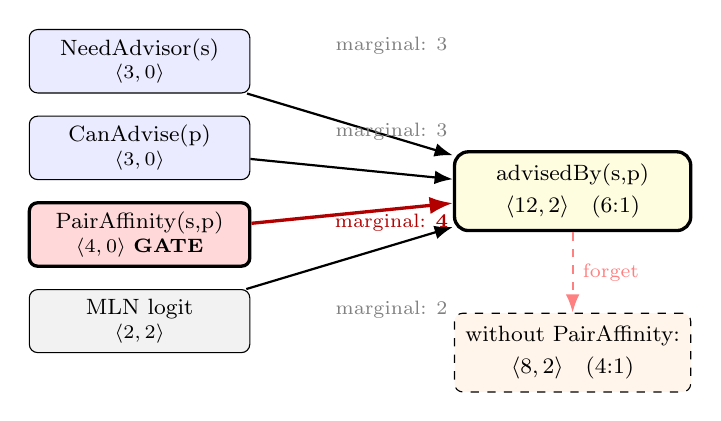
\begin{tikzpicture}[
  >=Latex,
  every node/.style={font=\footnotesize},
  role/.style={draw, rounded corners=3pt, minimum width=28mm,
               minimum height=8mm, align=center},
  target/.style={draw, very thick, rounded corners=5pt,
                 minimum width=30mm, minimum height=10mm,
                 align=center, fill=yellow!12},
  gate/.style={role, fill=red!15, very thick},
]
  \node[role, fill=blue!8] (need) at (0, 2.2)
    {NeedAdvisor(s)\\[-1pt]\scriptsize $\langle 3, 0 \rangle$};
  \node[role, fill=blue!8] (can) at (0, 1.1)
    {CanAdvise(p)\\[-1pt]\scriptsize $\langle 3, 0 \rangle$};
  \node[gate] (pair) at (0, 0)
    {PairAffinity(s,p)\\[-1pt]\scriptsize $\langle 4, 0 \rangle$
     \textbf{GATE}};
  \node[role, fill=gray!10] (mln) at (0, -1.1)
    {MLN logit\\[-1pt]\scriptsize $\langle 2, 2 \rangle$};

  \node[target] (pred) at (5.5, 0.55)
    {advisedBy(s,p)\\[2pt]
     $\langle 12, 2 \rangle$ \; ($6{:}1$)};

  \draw[->, thick] (need) -- (pred);
  \draw[->, thick] (can) -- (pred);
  \draw[->, very thick, red!70!black] (pair) -- (pred);
  \draw[->, thick] (mln) -- (pred);

  % Marginal annotations
  \node[font=\scriptsize, text=gray] at (3.2, 2.4) {marginal: 3};
  \node[font=\scriptsize, text=gray] at (3.2, 1.3) {marginal: 3};
  \node[font=\scriptsize, text=red!70!black]
    at (3.2, 0.15) {marginal: \textbf{4}};
  \node[font=\scriptsize, text=gray] at (3.2, -0.95) {marginal: 2};

  % Gate effect
  \node[draw, dashed, rounded corners=3pt, fill=orange!8,
        minimum width=30mm, minimum height=10mm, align=center]
    (gated) at (5.5, -1.5)
    {without PairAffinity:\\[2pt]
     $\langle 8, 2 \rangle$ \; ($4{:}1$)};
  \draw[->, dashed, thick, red!50] (pred) -- node[right,
    font=\scriptsize] {forget} (gated);
\end{tikzpicture}
\caption{UW-CSE advisedBy evidence roles.  PairAffinity
  (red, marginal contribution~4) is the compatibility gate:
  without it, the prediction drops from $6{:}1$ to $4{:}1$.
  Strong unary signals alone are insufficient.}
\label{fig:uwcse-gate}
\end{figure}

\noindent
With all four roles, the aggregate is $\langle 12, 2 \rangle$
for advisedBy---a $6{:}1$ ratio.  The compatibility gate
operates via \code{forget}: removing PairAffinity drops the
aggregate to $\langle 8, 2 \rangle$ ($4{:}1$).  The marginal
contributions---PairAffinity ($4$) $>$ NeedAdvisor ($3$) $=$
CanAdvise ($3$) $>$ MLN logit ($2$)---show that pairwise
interaction evidence is the critical discriminator.

\emph{Strong unary signals alone---a promising student and an
active professor---are insufficient for confident edge prediction
without pairwise evidence that they actually interact.}  This is
the same \code{forget} pattern that identified IASP as the
critical discriminator in the Pain reclassification
(\S\ref{sec:pain-evidence-wm}) and stale reliability weights as
the bottleneck in GJP forecasting
(\S\ref{sec:gjp-forecasting}).%
\footnote{Formalized in
\codepath{Mettapedia/Logic/WMUWCSEGateDemo.lean}
(177~lines, 12~theorems, 0~sorry).  The social-smoking benchmark
is in \codepath{Mettapedia/Logic/MarkovLogicUWCSE.lean}.}

\paragraph{Full benchmark results.}
On the full UW-CSE dataset (5-fold leave-one-area-out), the
compatibility-gated model improves over the MLN baseline on all
metrics:

\begin{table}[htbp]
\centering
\caption{MLN baseline vs.\ compatibility-gated WM model
  (leave-one-area-out, 5 folds).}
\label{tab:uwcse-gate-results}
\footnotesize
\begin{tabular}{l cc cc cc}
\toprule
& \multicolumn{2}{c}{AUROC} & \multicolumn{2}{c}{Hits@1}
& \multicolumn{2}{c}{Set-F1} \\
\cmidrule(lr){2-3}\cmidrule(lr){4-5}\cmidrule(lr){6-7}
Fold & MLN & Gate & MLN & Gate & MLN & Gate \\
\midrule
ai       & 0.845 & 0.871 & 0.433 & 0.433 & 0.389 & 0.411 \\
graphics & 0.884 & 0.932 & 0.071 & 0.357 & 0.048 & 0.381 \\
language & 0.871 & 0.893 & 0.375 & 0.375 & 0.333 & 0.333 \\
systems  & 0.845 & 0.872 & 0.444 & 0.593 & 0.395 & 0.531 \\
theory   & 0.866 & 0.916 & 0.500 & 0.417 & 0.417 & 0.389 \\
\midrule
Mean & 0.862 & \textbf{0.897} & 0.365 & \textbf{0.435}
     & 0.316 & \textbf{0.409} \\
\bottomrule
\end{tabular}
\end{table}

\noindent
The improvement is not from adding data---it is from
\emph{factoring} the existing clause-weight signal into
interpretable evidence roles.  The gains are concentrated on
folds where the MLN's pairless false-positive rate is highest
(graphics: 88\%, theory: 80\%).

\maplecourt{%
Maple Court's building model can be expressed as an MLN:
``\emph{If wall humidity is high, mold risk is elevated}''
with weight $w = 2.1$.  The WM decomposition factors this into
a BN-compatible evidence contribution (the chain
WallHumidity $\to$ MoldRisk) and a residual.  The compatibility
gate certifies that the chain structure holds, licensing the
compiled deduction rewrite.}

\paragraph{The semantic pipeline: from specification to truth value.}
The full chain from an infinite MLN specification to a PLN truth value
passes through four stages.  Each stage is a single, sorry-free Lean
definition or theorem; together they form the return map from Gibbs
semantics back into the algebraic WM interface.

\begin{figure}[htbp]
\centering
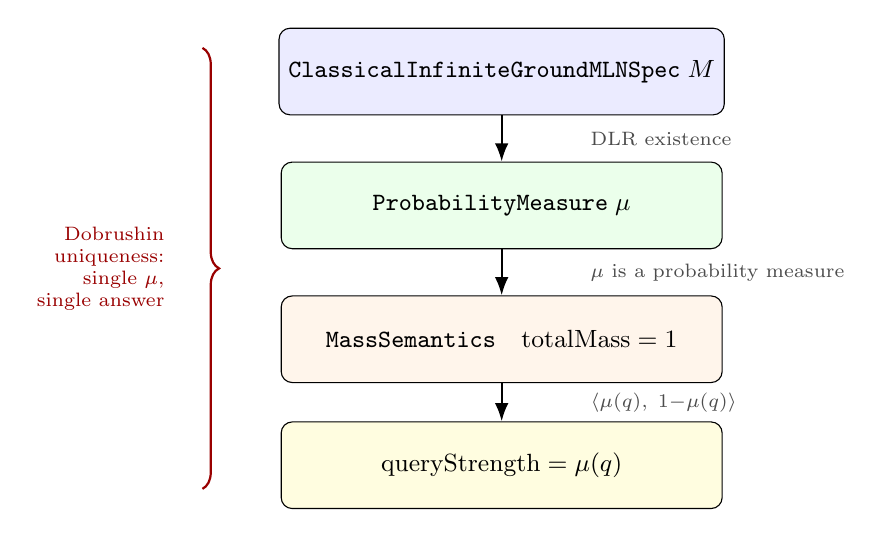
\begin{tikzpicture}[
  >=Latex,
  every node/.style={font=\small},
  stage/.style={draw, rounded corners=4pt, minimum width=56mm,
               minimum height=11mm, align=center},
  arrow/.style={->, thick},
  note/.style={font=\scriptsize, text=gray!60!black, align=left},
]
  \node[stage, fill=blue!8] (spec) at (0, 5.0)
    {\texttt{ClassicalInfiniteGroundMLNSpec}\;$M$};
  \node[stage, fill=green!8] (meas) at (0, 3.3)
    {\texttt{ProbabilityMeasure}\;$\mu$};
  \node[stage, fill=orange!8] (mass) at (0, 1.6)
    {\texttt{MassSemantics}\quad
     $\mathrm{totalMass} = 1$};
  \node[stage, fill=yellow!12] (wm) at (0, 0)
    {$\mathrm{queryStrength} = \mu(q)$};

  \draw[arrow] (spec) -- (meas)
    node[midway, right=10mm, note] {DLR existence};
  \draw[arrow] (meas) -- (mass)
    node[midway, right=10mm, note] {$\mu$ is a probability measure};
  \draw[arrow] (mass) -- (wm)
    node[midway, right=10mm, note]
    {$\langle\mu(q),\;1{-}\mu(q)\rangle$};

  % Uniqueness brace
  \draw[thick, red!60!black, decorate,
        decoration={brace, amplitude=6pt, mirror}]
    (-3.8, -0.3) -- (-3.8, 5.3)
    node[midway, left=10pt, font=\scriptsize, text=red!60!black, align=right]
    {Dobrushin\\uniqueness:\\single $\mu$,\\single answer};
\end{tikzpicture}
\caption{The infinite MLN $\to$ WM semantic pipeline.  Each arrow is a
  Lean definition or theorem; the left brace marks the scope of the
  Dobrushin uniqueness guarantee.}
\label{fig:infinite-mln-pipeline}
\end{figure}

\paragraph{Worked example: the infinite belief line.}
Consider an unbounded chain of agents indexed by $\mathbb{N}$, each holding a
Boolean belief.  A soft prior clause favors belief at every site, and a soft
influence clause
\[
  \mathrm{Believes}(n) \;\to\; \mathrm{Believes}(n{+}1)
\]
couples each pair of adjacent agents.  (The logical direction of the implication
does not limit the statistical interaction: at the Dobrushin level, flipping
either agent's value shifts the other's conditional probability.)  No finite
truncation captures the full system: cutting at~$N$ introduces an artificial
boundary whose choice affects marginals near the cut.

The infinite MLN formalization resolves this in three stages:
\begin{enumerate}
\item \textbf{Existence.}  A global Gibbs measure exists for the entire chain,
  and resampling the neighborhood around site~$n$ preserves the marginal belief
  probability at~$n$ (local DLR consistency).
\item \textbf{Uniqueness.}  If the influence weight satisfies $|w| < 1$, the
  Dobrushin row sum is uniformly bounded by~$|w|$, and the global measure is
  the only one.  For example, $w = 0.4$ means each neighbor multiplies belief
  odds by about $e^{0.4} \approx 1.49$---strong enough to matter, with total
  incoming influence 0.4 per agent, well within the budget.
\item \textbf{WM bridge.}  The unique Gibbs measure feeds into the pipeline of
  Figure~\ref{fig:infinite-mln-pipeline}: the WM query strength for any finite
  query (e.g., ``does agent~42 believe?'') is uniquely determined by the
  specification alone.
\end{enumerate}
\noindent
The corresponding negative example is equally instructive.  The original
``triple the odds'' influence weight $w = \log 3 \approx 1.1$ exceeds the
Dobrushin budget.  Existence still holds, but the uniqueness theorem no longer
applies: two boundary conditions at infinity could in principle yield different
global measures.%
\footnote{Formalized as
\code{exists\_beliefLine\_fixedRegionCylinderDLR},
\code{beliefLineClassicalSpec\_uniformSmallTotalInfluence},
\code{beliefLine\_uniqueMeasure}, and
\code{beliefLine\_wmBridge\_unique} in
\codepath{Mettapedia/Logic/MarkovLogicInfiniteBeliefLineExample.lean}
(0~sorry).}

\paragraph{Applications: where infinite MLNs arise naturally.}
The belief line is a proxy for any system whose relational structure has no
natural finite boundary:

\smallskip\noindent\textbf{Physical systems.}
\begin{description}
\item[Apartment corridors.]  Humidity in unit~$n$ raises mold risk in
  unit~$n{+}1$.  Query: risk at apartment~42, without pretending the building
  stops at some arbitrary wall.
\item[2D sensor grids.]  Sensor fields, floor plans, and crop lattices
  on $\mathbb{N}\times\mathbb{N}$.  Each interior node has four neighbours;
  the uniqueness budget becomes $2|w|<1$.
\item[Supply-chain cascades.]  Delay at stage~$n$ raises disruption risk at
  stage~$n{+}1$.  Query: disruption probability at depot~50.
\end{description}

\smallskip\noindent\textbf{Social systems.}
\begin{description}
\item[Rumor and trust relays.]  Agent~$n$ adopting a claim nudges
  agent~$n{+}1$.  Query: the probability that the claim reaches reviewer~100.
\item[Worlds of views~\cite{VeitasWeinbaum2015}.]  Agents with heterogeneous
  priors and directed trust weights.  The bidirectional variant allows mutual
  reinforcement or skepticism, as long as the combined trust budget remains
  uniformly subcritical.
\item[Variable-neighborhood sense-making.]  A countable agent society with
  finite but nonuniform local neighborhoods.  Some agents trust three peers,
  some one, some none; uniqueness still follows whenever each agent's total
  incoming-plus-outgoing trust budget remains uniformly below~1.
\end{description}

\smallskip\noindent\textbf{Computational / AGI systems.}
\begin{description}
\item[Open-ended knowledge graphs.]  New concepts keep arriving.  The theorem
  does not require the graph to be finite in advance; it only requires that
  each node's incoming interaction budget stay uniformly controlled.
\item[Bounded-degree concept ladders.]  Two infinite concept tracks with local
  inheritance and bounded cross-track bridges.
\end{description}

\begin{figure}[htbp]
\centering
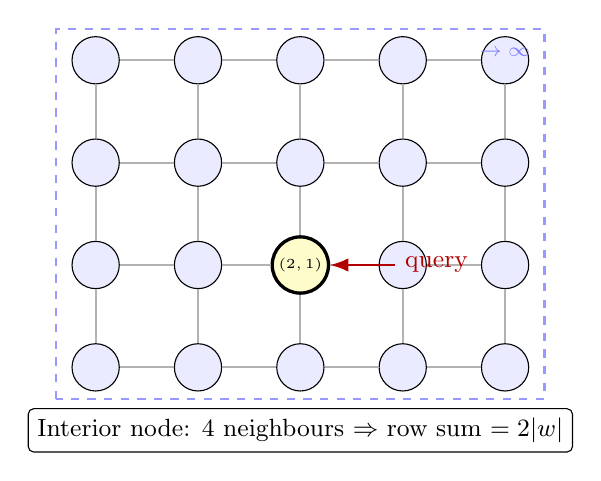
\begin{tikzpicture}[
  >=Latex,
  every node/.style={font=\footnotesize},
  site/.style={circle, draw, inner sep=1.5pt, minimum size=6mm, fill=blue!8},
  query/.style={circle, draw, very thick, inner sep=1.5pt, minimum size=6mm,
                fill=yellow!20},
  edge/.style={-, thick, gray!60},
]
  % Grid nodes
  \foreach \i in {0,...,4} {
    \foreach \j in {0,...,3} {
      \pgfmathtruncatemacro{\isquery}{ifthenelse(\i==2 && \j==1, 1, 0)}
      \ifnum\isquery=1
        \node[query] (n\i\j) at (1.3*\i, 1.3*\j) {\tiny $(\i,\j)$};
      \else
        \node[site] (n\i\j) at (1.3*\i, 1.3*\j) {};
      \fi
    }
  }
  % Horizontal edges
  \foreach \i [evaluate=\i as \inext using int(\i+1)] in {0,...,3} {
    \foreach \j in {0,...,3} {
      \draw[edge] (n\i\j) -- (n\inext\j);
    }
  }
  % Vertical edges
  \foreach \i in {0,...,4} {
    \foreach \j [evaluate=\j as \jnext using int(\j+1)] in {0,...,2} {
      \draw[edge] (n\i\j) -- (n\i\jnext);
    }
  }
  % Budget annotation
  \node[draw, rounded corners=2pt, fill=white, font=\small] at (2.6, -0.8)
    {Interior node: 4 neighbours $\Rightarrow$ row sum $= 2|w|$};
  % Query annotation
  \draw[->, thick, red!70!black] (3.8, 1.3) -- (n21)
    node[pos=0, right, font=\small, text=red!70!black] {query};
  % Boundary annotation
  \draw[dashed, thick, blue!40] (-0.5, -0.4) rectangle (5.7, 4.3);
  \node[font=\scriptsize, text=blue!50] at (5.2, 4.0) {$\to \infty$};
\end{tikzpicture}
\caption{The 2D grid MLN on $\mathbb{N}\times\mathbb{N}$.  Each interior
  node (blue) has four nearest neighbours.  The yellow node marks a query
  site; the dashed boundary recedes to infinity.  Under $2|w|<1$, the
  query probability is uniquely determined.}
\label{fig:grid-mln}
\end{figure}

\noindent
The 2D grid makes the \emph{dimensional cost} of interaction concrete.  With
$w = 0.2$ (each neighbour multiplies odds by $e^{0.2}\approx 1.22$), the
Dobrushin budget is $2\times 0.2 = 0.4$, safely below~$1$.  The probability
that sensor~$(15,23)$ reads high is uniquely determined by the specification,
regardless of boundary conditions at infinity.  But with $w = 0.6$, the budget
$2\times 0.6 = 1.2$ exceeds the threshold---this is the regime of the
classical 2D Ising model at low temperature, the most studied phase transition
in all of statistical mechanics.  Existence of a Gibbs measure still holds, but
the proved uniqueness theorem no longer applies: coexisting $+$ and $-$
equilibria become possible.%
\footnote{Formalized in
\codepath{Mettapedia/Logic/MarkovLogicInfiniteGridExample.lean}
(430~lines, 0~sorry).  The proof reuses the full pipeline:
\code{gridClassicalSpec\_uniformSmallTotalInfluence},
\code{grid\_uniqueMeasure},
\code{grid\_wmBridge\_unique}.}

\medskip
\noindent
In each case the infinite MLN formalization answers the same question:
\emph{when do local log-linear interaction laws compose into a coherent global
semantics, rather than merely a sequence of finite approximations?}

\paragraph{Open-ended ontology stability.}
There are now two formal layers to the ontology-growth story.

First, the descending-shell contraction argument yields a reusable
same-specification stability theorem.  If a finite query region $\Delta$ sits
inside a countably infinite knowledge graph satisfying the uniform Dobrushin
budget $C < 1$, then disagreement between two admissible DLR completions of
that \emph{same} specification decays geometrically with shell depth:
\[
  \mathrm{TV}_{\Delta}(\mu,\nu) \;\le\; |\Delta|\,C^n,
  \qquad
  \bigl|\Pr_{\mu}(q)-\Pr_{\nu}(q)\bigr|
  \;\le\; 2\,|\Delta|\,C^n
\]
after $n$ interaction-neighborhood shells.  This is the precise formal
content behind the slogan that an ontology may keep growing ``at infinity''
while local query answers remain stable, provided every node's incoming
interaction budget stays uniformly subcritical.%
\footnote{Formalized in
\codepath{Mettapedia/Logic/MarkovLogicInfiniteBoundaryStability.lean}
via
\code{finiteRegionAssignmentTotalVariation\_le\_geometric\_of\_uniformSmallTotalInfluence}
and
\code{finiteRegionLocalQueryDiscrepancy\_le\_geometric\_of\_uniformSmallTotalInfluence}
(0~sorry).}

\noindent
Second, the cross-specification ontology-growth theorem now proves the exact
invariance claim that motivated the section.  If two MLN specifications agree
on every clause touching an interaction-closed region $\Gamma$ containing the
query atoms, then adding or modifying clauses \emph{outside} that zone does
not change the query answer at all:
\[
  \Pr_{M_1,\mu_1}(q) \;=\; \Pr_{M_2,\mu_2}(q).
\]
This is stronger than shell decay.  It says that once the local clause support
is literally unchanged, the finite-volume Gibbs kernel on $\Gamma$ is
identical, and the DLR equation forces exact local agreement.%
\footnote{Formalized in
\codepath{Mettapedia/Logic/MarkovLogicOntologyGrowth.lean}
via
\code{agreesOnBoundarySupport\_of\_interactionClosed},
\code{finiteVolumeQueryProb\_eq\_of\_specAgreesOnRegion},
and
\code{queryProb\_stable\_of\_extension\_outside}
(0~sorry).}

\begin{figure}[htbp]
\centering
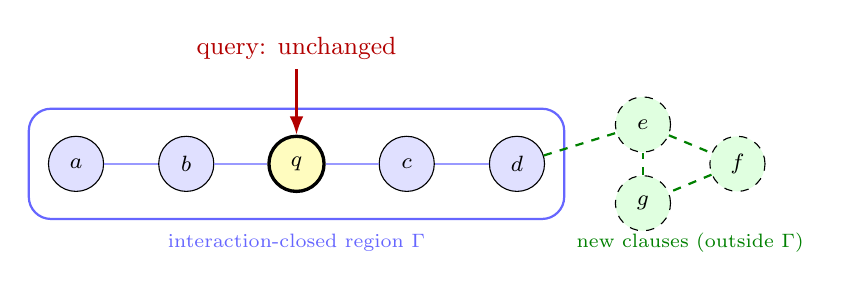
\begin{tikzpicture}[
  >=Latex,
  every node/.style={font=\footnotesize},
  old/.style={circle, draw, fill=blue!12, inner sep=2pt, minimum size=7mm},
  new/.style={circle, draw, dashed, fill=green!12, inner sep=2pt, minimum size=7mm},
  query/.style={circle, draw, very thick, fill=yellow!25, inner sep=2pt, minimum size=7mm},
  oldedge/.style={-, thick, blue!40},
  newedge/.style={-, thick, dashed, green!50!black},
]
  % Old spec atoms
  \node[old] (a) at (0, 0) {$a$};
  \node[old] (b) at (1.4, 0) {$b$};
  \node[query] (q) at (2.8, 0) {$q$};
  \node[old] (c) at (4.2, 0) {$c$};
  \node[old] (d) at (5.6, 0) {$d$};

  % Old edges
  \draw[oldedge] (a) -- (b);
  \draw[oldedge] (b) -- (q);
  \draw[oldedge] (q) -- (c);
  \draw[oldedge] (c) -- (d);

  % Interaction-closed region
  \draw[rounded corners=8pt, thick, blue!60]
    (-0.6, -0.7) rectangle (6.2, 0.7);
  \node[font=\scriptsize, text=blue!60] at (2.8, -1.0)
    {interaction-closed region $\Gamma$};

  % New atoms added outside
  \node[new] (e) at (7.2, 0.5) {$e$};
  \node[new] (f) at (8.4, 0) {$f$};
  \node[new] (g) at (7.2, -0.5) {$g$};

  % New edges (only among new atoms, or to d at boundary)
  \draw[newedge] (d) -- (e);
  \draw[newedge] (e) -- (f);
  \draw[newedge] (f) -- (g);
  \draw[newedge] (g) -- (e);

  % Labels
  \node[font=\scriptsize, text=green!50!black] at (7.8, -1.0)
    {new clauses (outside $\Gamma$)};
  \draw[->, thick, red!70!black] (2.8, 1.2) -- (q)
    node[pos=0, above, font=\small, text=red!70!black]
    {query: unchanged};
\end{tikzpicture}
\caption{Ontology growth stability.  The query node $q$ sits inside the
  interaction-closed region $\Gamma$ (blue).  New atoms $e,f,g$ and their
  clauses (green, dashed) are added outside $\Gamma$.  Since no new clause
  touches $\Gamma$'s interior, the cross-specification theorem guarantees
  the query probability is exactly preserved.}
\label{fig:ontology-growth}
\end{figure}

\noindent
Positive example: adding far-away schema refinements to a bounded-interaction
knowledge graph leaves every local query exactly unchanged
(Figure~\ref{fig:ontology-growth}).
Negative example: if a newly added hub concept injects a clause \emph{into}
the query region's interaction neighbourhood, exact agreement fails
immediately; and if the total incoming budget becomes unbounded, even the
geometric stability theorem no longer applies.

\paragraph{Individuated subsystems and the capstone theorem.}
The ontology-growth and boundary-stability results can be bundled into a
single concept that connects to the philosophical literature on open-ended
intelligence: an \emph{individuated subsystem}~\cite{WeinbaumVeitas2015}.
An interaction-closed region $\Gamma$ of an infinite MLN has three formal
properties that together constitute a rigorous analogue of
Simondon--Weinbaum individuation:
\begin{enumerate}
\item \textbf{Query stability.}  Any query supported on $\Gamma$ has
  answer-discrepancy that decays geometrically with shell depth:
  $|\Pr_\mu(q) - \Pr_\nu(q)| \le 2|\Gamma|C^n$.
\item \textbf{Ontology robustness.}  Adding clauses outside $\Gamma$ does
  not change the subsystem's query answers --- exactly, not approximately.
\item \textbf{WM bridge uniqueness.}  The subsystem's truth values
  ($\mathrm{queryStrength} = \mu(q)$) are specification-determined under
  the Dobrushin budget.
\end{enumerate}
Together these say: an individuated subsystem has a \emph{stable identity}
(its query answers) that \emph{persists under perturbation} (ontology growth)
and is \emph{uniquely determined} (Dobrushin uniqueness).

The capstone theorem makes the WM punchline fully explicit:

\begin{theorem}[WM truth-value stability under ontology extension (\claimConditional{})]
\label{thm:wm-ontology-stability}
Let $\Gamma$ be an individuated subsystem (interaction-closed, nonempty) of two
infinite MLN specifications $M_1, M_2$ that agree on all clauses touching
$\Gamma$ and both satisfy the uniform Dobrushin budget.  Then for every
query $q$ supported on $\Gamma$:
\[
  \mathrm{queryStrength}_{M_1}(q) \;=\; \mathrm{queryStrength}_{M_2}(q).
\]
In particular, adding or modifying clauses outside the protected core does not
change the WM truth value of any query inside it.%
\footnote{Formalized as
\code{wmStrength\_stable\_under\_extension} in
\codepath{Mettapedia/Logic/MarkovLogicIndividuation.lean}
(0~sorry).  The proof composes ontology-growth invariance with the
\texttt{MassState.queryStrength\_singleton\_eq\_queryProb} bridge.}
\end{theorem}

\noindent
This is the formal content behind the ``open-ended intelligence''
desideratum of Weinbaum and Veitas~\cite{WeinbaumVeitas2015}: a system that
keeps generating new structure without collapsing the coherence of existing
knowledge.  The Dobrushin budget is the quantitative price of coherence;
the individuated subsystem is its formal manifestation; and the capstone
theorem says that the price is paid at the level of WM truth values, not just
raw probabilities.
In Weinbaum and Veitas's terminology~\cite{WeinbaumVeitas2015}, the
interaction-closed region plays the role of a \emph{domain-relative ground}:
the minimal stable locus from which the subsystem's identity is constituted.
The Dobrushin budget is the quantitative counterpart of Simondon's
transductive tension --- it bounds how much the exterior can influence the
interior without destabilising it.

The formalization captures the \emph{static criterion} for individuation ---
when a subsystem IS individuated.%
\footnote{Formalized in
\codepath{Mettapedia/Logic/MarkovLogicIndividuation.lean}
via \code{IndividuatedSubsystem}, \code{queryDiscrepancy\_le\_geometric},
\code{queryProb\_invariant\_under\_extension},
\code{wmQueryStrength\_unique}, and the capstone
\code{wmStrength\_stable\_under\_extension} (0~sorry).}

\paragraph{Dynamic individuation: boundary emergence with shell guarantees.}

The \emph{process} by which an individuated subsystem emerges is now
also formalized.  A \emph{proto-core} is a finite nonempty seed region before
full interaction-closure is known.  A \emph{dynamic individuation step}
tracks distant rewrites that maintain shell agreement around the seed; each
step contributes $2|\mathrm{seed}|\,C^n$ to the cumulative drift.  A
\emph{dynamic individuation path} is a coherent chain of such steps with a
proved cumulative WM-drift bound.  The key transition: once the shell around
the seed is interaction-closed, a \code{DynamicIndividuationClosure}
promotes the path to \emph{exact} invariance --- seed-supported queries
are thereafter exactly preserved under further extension.%
\footnote{Formalized in
\codepath{Mettapedia/Logic/MarkovLogicDynamicIndividuation.lean}
via \code{ProtoCore}, \code{DynamicIndividuationStep},
\code{DynamicIndividuationPath},
\code{seed\_wmStrength\_cumulative\_drift},
\code{DynamicIndividuationClosure}, and the exact post-closure
theorems \code{seed\_queryProb\_exact\_under\_extension} and
\code{seed\_wmStrength\_exact\_under\_extension} (0~sorry).}

\noindent
Positive example: a subsystem boundary is not fully settled yet, but the
system keeps shell agreement around a seed; local seed queries drift only by
geometric tails until closure is reached, after which they are exactly
stable.
Negative example: if shell agreement is violated near the seed, or Dobrushin
budgets fail, no stability guarantee is provided.

\paragraph{Coupled subsystems inside one protected carrier.}

The next social step is not yet ``compassion'' in any thick ethical sense,
but it is already a mathematically meaningful two-community theorem.  A
single interaction-closed carrier $\Omega$ may contain two disjoint
nonempty local cores $\Gamma_L$ and $\Gamma_R$, together with an interface
region $\Omega \setminus (\Gamma_L \cup \Gamma_R)$ through which the two
communities may influence one another.  The individual cores need not be
interaction-closed on their own; what is protected is the larger carrier.
If a second specification agrees with the first on $\Omega$ and both satisfy
the Dobrushin budget, then every query supported on $\Gamma_L$, every query
supported on $\Gamma_R$, and every joint query supported on
$\Gamma_L \cup \Gamma_R$ has exactly the same Gibbs probability and hence
the same WM truth value in both specifications.%
\footnote{Formalized in
\codepath{Mettapedia/Logic/MarkovLogicCoupledSubsystems.lean}
via \code{CoupledSubsystems},
\code{left\_queryProb\_invariant\_under\_extension},
\code{right\_queryProb\_invariant\_under\_extension},
\code{coupled\_queryProb\_invariant\_under\_extension}, and the
corresponding WM theorems (0~sorry).}
This is the precise sense in which two local ``worlds of views'' can form
one protected social carrier: the interface may mediate interaction, but
distant ontology growth outside the carrier does not alter either side's
local or joint truth values.
In the ``world of views'' framework of Veitas and
Weinbaum~\cite{VeitasWeinbaum2017}, this formalises the coexistence of
multiple local perspectives inside one shared social carrier: each community
retains its own semantic ground, and the carrier acts as the ecology in which
they interact without either perspective being overwritten by the other.
The social-individuation work of Lenartowicz and
Weinbaum~\cite{LenartowiczWeinbaum2016} provides the sociological motivation
for this topology.

\paragraph{Dynamic coupled subsystems.}

The exact carrier theorem has a dynamic counterpart.  If two specifications
agree not merely on the protected carrier $\Omega$ but on its $n$-shell
\(\mathrm{iterExpandRegion}(\Omega,n)\), then left-local, right-local, and
joint carrier queries differ by at most \(2|\Omega|C^n\).  The full carrier
\(\Omega\), not just the smaller left or right community, appears in the
bound because the Dobrushin contraction runs on the protected carrier shell.
This is the
coupled-community version of dynamic self-transcendence: distant rewriting
outside the shared carrier perturbs both communities only by a geometric
tail.%
\footnote{Formalized in
\codepath{Mettapedia/Logic/MarkovLogicDynamicCoupledSubsystems.lean}
via \code{DynamicCoupledSubsystemStep} and the left/right/joint
\code{...\_approximately\_preserved} theorems, together with the path
theorems \code{left\_queryProb\_cumulative\_drift},
\code{right\_queryProb\_cumulative\_drift},
\code{coupled\_queryProb\_cumulative\_drift}, and their WM corollaries
(0~sorry).}

\paragraph{Worked example: two communities with a liaison layer.}

A concrete carrier example is now formalized as well.  Agents
\(\{0,1\}\) form the left community, agent \(\{2\}\) is the interface,
agents \(\{3,4\}\) form the right community, and an external tail
\(\{5,6,7,\ldots\}\) is disconnected from the carrier.  The protected
carrier is therefore \(\Omega = \{0,1,2,3,4\}\).  Two specifications may
share the carrier weight \(w_c\) while assigning different tail weights
\(w_{t1}\) and \(w_{t2}\); nevertheless, every joint query supported on the
two communities has exactly the same WM truth value in both specifications.
This example uses the stronger exact theorem, not merely the dynamic bound,
because the carrier itself is interaction-closed and the tail is fully
disconnected.%
\footnote{Formalized in
\codepath{Mettapedia/Logic/MarkovLogicCoupledCommunitiesExample.lean}
via \code{coupledCommunities\_joint\_wmStrength\_stable} (0~sorry).}

\paragraph{Worked capstone: a protected trust triangle.}

\begin{figure}[htbp]
\centering
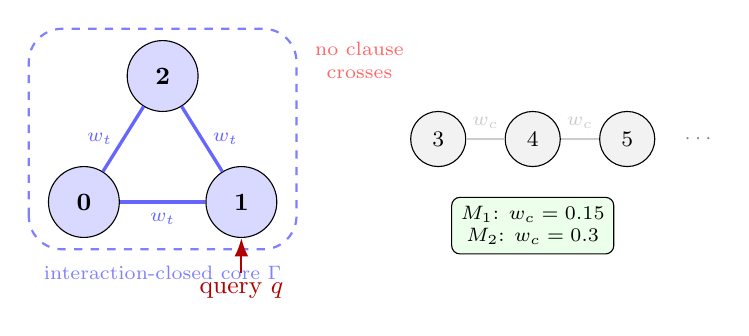
\begin{tikzpicture}[
  >=Latex,
  every node/.style={font=\footnotesize},
  agent/.style={circle, draw, fill=blue!15, inner sep=2pt, minimum size=9mm,
                font=\small\bfseries},
  chain/.style={circle, draw, fill=gray!10, inner sep=2pt, minimum size=7mm},
  trust/.style={-, very thick, blue!60},
  chainedge/.style={-, thick, gray!40},
  querylabel/.style={font=\small, text=red!70!black},
]
  % Trust triangle
  \node[agent] (a0) at (0, 0) {0};
  \node[agent] (a1) at (2, 0) {1};
  \node[agent] (a2) at (1, 1.6) {2};

  \draw[trust] (a0) -- (a1) node[midway, below, font=\scriptsize] {$w_t$};
  \draw[trust] (a1) -- (a2) node[midway, right, font=\scriptsize] {$w_t$};
  \draw[trust] (a2) -- (a0) node[midway, left, font=\scriptsize] {$w_t$};

  % Interaction-closed boundary
  \draw[rounded corners=12pt, thick, blue!50, dashed]
    (-0.7, -0.6) rectangle (2.7, 2.2);
  \node[font=\scriptsize, text=blue!50] at (1, -0.9)
    {interaction-closed core $\Gamma$};

  % Chain (disconnected)
  \node[chain] (c3) at (4.5, 0.8) {3};
  \node[chain] (c4) at (5.7, 0.8) {4};
  \node[chain] (c5) at (6.9, 0.8) {5};
  \node[font=\scriptsize, text=gray] at (7.8, 0.8) {$\cdots$};

  \draw[chainedge] (c3) -- (c4) node[midway, above, font=\scriptsize] {$w_c$};
  \draw[chainedge] (c4) -- (c5) node[midway, above, font=\scriptsize] {$w_c$};

  % No connection between triangle and chain
  \node[font=\scriptsize, text=red!60, align=center] at (3.5, 1.8)
    {no clause\\crosses};

  % Query arrow
  \draw[->, thick, red!70!black] (2.0, -0.9) -- (a1)
    node[pos=0, below, querylabel] {query $q$};

  % Spec labels
  \node[draw, rounded corners=3pt, fill=green!8, font=\scriptsize,
        align=center] at (5.7, -0.3)
    {$M_1$: $w_c = 0.15$\\$M_2$: $w_c = 0.3$};
\end{tikzpicture}
\caption{The trust triangle.  Agents $\{0,1,2\}$ form an interaction-closed
  core (blue, dashed boundary).  A separate, \emph{fully disconnected} infinite
  chain $\{3,4,5,\ldots\}$ shares no edges or clauses with the triangle ---
  there is no path from any chain node to any triangle node.
  Specifications $M_1$ and $M_2$ use the same triangle weight $w_t$ but assign
  different chain weights ($w_{c1} \neq w_{c2}$).  Because the chain is
  disconnected, the triangle is interaction-closed and the theorem gives exact
  preservation:
  $\mathrm{queryStrength}_{M_1}(q) = \mathrm{queryStrength}_{M_2}(q)$
  for every query $q$ supported on the triangle.}
\label{fig:trust-triangle}
\end{figure}

\noindent
The generic theorem above is now instantiated by a concrete Lean example.
Let $\Gamma = \{0,1,2\}$ be a trust triangle with internal weight $w_t$.
Outside the triangle sits an infinite trust chain, with chain weight $w_{c1}$
under specification $M_1$ and $w_{c2}$ under specification $M_2$.  The two
specifications agree exactly on the triangle and may differ arbitrarily on the
tail.  Let $q$ be the query ``does agent~1 endorse the claim?''  Then, under
$|w_t|<\tfrac12$, $|w_{c1}|<\tfrac12$, and $|w_{c2}|<\tfrac12$:
\begin{enumerate}
\item Both $M_1$ and $M_2$ admit DLR measures (existence).
\item Both satisfy the Dobrushin budget (uniform contraction).
\item The DLR measures are unique for each spec (uniqueness).
\item The WM query strength of $q$ is $\mu_1(q)$ for $M_1$ and $\mu_2(q)$
  for $M_2$ (bridge).
\item Since $M_1$ and $M_2$ agree on $\Gamma$ and $\Gamma$ is
  interaction-closed, Theorem~\ref{thm:wm-ontology-stability} gives
  $\mathrm{queryStrength}_{M_1}(q) = \mathrm{queryStrength}_{M_2}(q)$.
\end{enumerate}
The distant new agents do not change agent~1's truth value.  This is the
formal content of
\code{trust\_triangle\_wmStrength\_stable} in
\codepath{Mettapedia/Logic/MarkovLogicTrustTriangleExample.lean}.
The threshold $\tfrac12$ is not cosmetic: in this directed trust model each
agent pays for both incoming and outgoing local influence, so the honest row
budget is $2|w|$, not $|w|$.  Positive example: with $w_t = 0.2$ and
$w_{c1}=w_{c2}=0.15$, the theorem applies.  Negative example: with
$w_t = 0.7$, the local triangle alone already lies outside the proved
uniqueness regime.

\paragraph{Self-transcendence as preserved identity under growth.}
The next step is no longer a single extension but a whole path of coherent
extensions.  A \emph{transcendence step} grows a specification while preserving
an old protected core.  A \emph{transcendence path} is a finite chain of such
steps together with a coherence condition saying that every later protected
core still contains the original one.  Under that hypothesis, the theorem
\code{TranscendencePath.original\_queries\_stable} proves that any query on the
\emph{original} core has exactly the same WM truth value at the end of the
path as it had at the start.  This is the formal analogue of static
self-transcendence in the Weinbaum--Veitas sense: the system may keep growing,
but its earlier identity is preserved rather than overwritten.  Positive
example: a community adds new collaborators and new topics while leaving its
founding trust core semantically intact.  Negative example: if a later growth
step rewrites clauses inside the original core, or if the path is not coherent,
exact preservation is no longer guaranteed by the theorem.%
\footnote{Formalized in
\codepath{Mettapedia/Logic/MarkovLogicSelfTranscendence.lean}
via \code{TranscendenceStep.old\_queries\_preserved} and
\code{TranscendencePath.original\_queries\_stable} (0~sorry).}

\paragraph{Meta-goal stability under proof-backed self-modification.}

The dynamic self-transcendence and coupled-subsystem theorems have a direct
application to the Schmidhuber
G\"odel-machine scenario: an agent that rewrites its own code only when a
machine-checked proof guarantees improvement.  The formalization packages
two results.%
\footnote{Formalized in
\codepath{Mettapedia/UniversalAI/GodelMachine/MetaGoalShellPreservation.lean}
(0~sorry).  The proof composes the G\"odel-machine utility-improvement
witness from \codepath{Mettapedia/UniversalAI/GodelMachine/Basic.lean}
with the Markov-logic individuation and dynamic-transcendence layers.}
\begin{enumerate}
\item \textbf{Exact preservation.}
  If the proof-backed rewrite leaves an interaction-closed protected core
  untouched, then every WM meta-goal query supported on that core keeps
  its truth value exactly, and expected utility strictly improves.
\item \textbf{Dynamic shell preservation.}
  If the rewrite stays outside the $n$-shell around a protected query
  region, then every meta-goal query drifts by at most $2|\Gamma|C^n$,
  and expected utility still strictly improves.
\end{enumerate}
\noindent
Positive example: a proof-backed rewrite of a remote planning module leaves
core medical or governance queries unchanged (exact case) or bounded by a
geometric tail (shell case) while certifiably improving utility.
Negative example: if the rewrite reaches the protected core itself, or the
Dobrushin budget fails, these theorems give no stability guarantee.

These single-step results compose into a \emph{meta-goal preservation path}:
a finite chain of proof-backed rewrites, each protecting the same query
region, with a coherence condition ensuring each later step still contains
the original protected goals.  Under that hypothesis, every meta-goal query
drifts by at most the sum of the step-wise shell tails, and expected utility
strictly improves at every step.%
\footnote{Formalized in
\codepath{Mettapedia/UniversalAI/GodelMachine/MetaGoalShellPreservationPath.lean}
via \code{MetaGoalShellPreservationPath},
\code{utility\_improves},
\code{goal\_wmStrength\_cumulative\_drift}, and the combined theorem
\code{validModification\_and\_goal\_wmStrength\_cumulative\_drift}
(0~sorry).}
This is now instantiated by a concrete two-step example on the trust
triangle: two successive proof-backed rewrites of the chain weights improve
utility while keeping a protected agent-1 query within a cumulative WM
drift bound of~$12$.%
\footnote{Formalized in
\codepath{Mettapedia/UniversalAI/GodelMachine/MetaGoalShellPreservationExample.lean}
via \code{trustTriangle\_twoStep\_metagoal\_preservation} (0~sorry).}

\paragraph{Anytime Solomonoff-to-WM approximation.}

A separate bridge connects the universal-prediction side to WM-style query
semantics.  A \emph{finite-prefix approximation} sums the first~$n$ programs
of the universal semi-measure, yielding a computable lower bound on any
prefix-event probability.  The formalization proves three properties of this
approximation ladder.%
\footnote{Formalized in
\codepath{Mettapedia/Logic/UniversalPredictionApproximation.lean} and
\codepath{Mettapedia/Logic/UniversalPredictionApproximationWMBridge.lean}
(0~sorry).}
\begin{enumerate}
\item \textbf{Monotonicity.}  Adding more programs to the prefix sum can only
  increase the approximate mass: if $m \le n$ then
  $\xi_m(x) \le \xi_n(x)$.
\item \textbf{Upper bound.}  Every finite-prefix mass is bounded by the full
  universal mixture: $\xi_n(x) \le \xi(x)$.
\item \textbf{WM score bridge.}  Each approximant feeds a
  \code{BinaryEvidence} record whose \code{toStrength} is the finite-prefix
  WM score.  Monotonicity and the upper bound transfer to these scores:
  increasing the budget can only raise the WM-style score, and never above
  the full universal-mixture score.
\end{enumerate}
\noindent
Positive example: a resource-bounded agent that enumerates $n$~programs
gets a WM-style truth value that improves monotonically with~$n$ and is
always a valid lower bound on the ideal Solomonoff score.

The prefix-event bridge extends to \emph{conditional queries}.  A
continuation query ``next bits are~$y$ given current prefix~$x$'' becomes a
\code{BinaryEvidence} record
$\langle\mu(x \mathbin{{+}{+}} y),\; \mu(x) - \mu(x \mathbin{{+}{+}} y)\rangle$
whose WM strength is exactly the semimeasure conditional
$\mu(y\,|\,x) = \mu(x \mathbin{{+}{+}} y) / \mu(x)$.  Both finite-prefix
and full-mixture conditional profiles are provided, together with their
geometric specialisations.%
\footnote{Formalized in
\codepath{Mettapedia/Logic/UniversalPredictionConditionalWMBridge.lean}
(0~sorry).}

\paragraph{Three-layer combined theorem.}

The meta-goal preservation path and the Solomonoff approximation ladder
can now be stated together in one theorem: a proof-backed rewrite path
strictly improves expected utility, protected WM meta-goals drift by at most
the cumulative shell-tail bound, and geometric universal-mixture prefix scores
improve monotonically with approximation budget and stay below the full
score.%
\footnote{Formalized in
\codepath{Mettapedia/UniversalAI/GodelMachine/MetaGoalUniversalApproximationBridge.lean}
(0~sorry).}

\noindent
Figure~\ref{fig:three-layer} illustrates the three layers and their proved
connections.

\begin{figure}[ht]
\centering
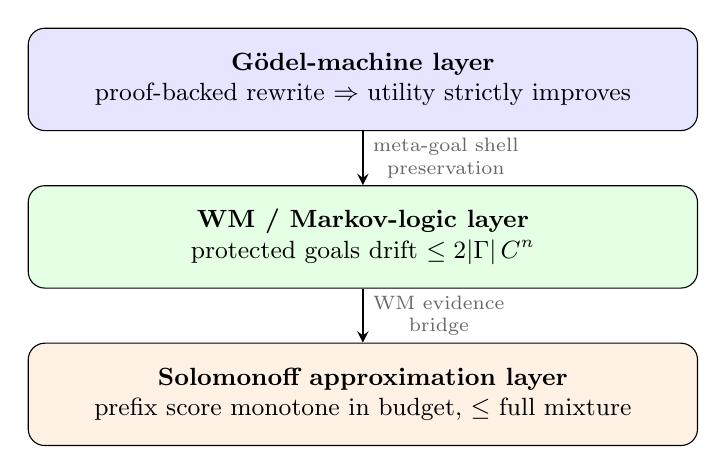
\begin{tikzpicture}[
  layer/.style={draw, rounded corners=6pt, minimum width=8.5cm,
    minimum height=1.3cm, align=center, font=\small},
  arr/.style={->, thick, >=stealth},
  note/.style={font=\scriptsize, text=black!60, align=center}
]
  \node[layer, fill=blue!10] (godel) at (0, 4.0)
    {\textbf{G\"odel-machine layer}\\proof-backed rewrite $\Rightarrow$
     utility strictly improves};
  \node[layer, fill=green!10] (wm) at (0, 2.0)
    {\textbf{WM / Markov-logic layer}\\protected goals drift
     $\le 2|\Gamma|\,C^n$};
  \node[layer, fill=orange!10] (sol) at (0, 0)
    {\textbf{Solomonoff approximation layer}\\prefix score monotone
     in budget, $\le$ full mixture};
  \draw[arr] (godel) -- (wm)
    node[midway, right, note] {meta-goal shell\\preservation};
  \draw[arr] (wm) -- (sol)
    node[midway, right, note] {WM evidence\\bridge};
\end{tikzpicture}
\caption{The three-layer architecture now proved in Lean.  A proof-backed
  rewrite (top) improves utility; the protected WM core drifts
  geometrically (middle); and anytime universal-mixture approximation
  improves monotonically with budget (bottom).  The combined theorem
  packages all three guarantees in one statement.}
\label{fig:three-layer}
\end{figure}

\noindent
Positive example: a self-modifying agent allocates more compute to its
universal predictor while rewriting a remote planning module; the combined
theorem guarantees utility improves, protected medical/governance goals stay
within the shell bound, and prediction scores get closer to the Solomonoff
ideal.
Negative example: the three layers are not yet identified --- the
universal-mixture score and the Markov-logic WM score are separate semantic
objects, and the theorem states both guarantees in conjunction, not as a
single unified semantics.

\paragraph{Conditional approximation and intensional inheritance.}

The prefix-event bridge extends further.  A quantitative error bound
is now proved for conditional approximants under an explicit denominator
floor: if the context probability $\mu_n(x) \ge \varepsilon$, then the
conditional error is at most the prefix error divided by $\varepsilon$.%
\footnote{Formalized in
\codepath{Mettapedia/Logic/UniversalPredictionConditionalApproximation.lean}
via \code{conditionalApproxError\_le\_of\_floor}
and the geometric specialisation
\code{geomConditionalQueryStrength\_approx\_error\_le\_of\_floor}
(0~sorry).}
This feeds the intensional-inheritance layer: approximate $P(W|F,x)$ and
$P(W|x)$ scores now give approximate intensional-inheritance strengths with a
proved error envelope that shrinks as the approximation budget
grows.%
\footnote{Formalized in
\codepath{Mettapedia/Logic/IntensionalInheritanceApproximationBridge.lean}
(0~sorry).}

A concrete end-to-end example instantiates the full bridge: a two-step
proof-backed rewrite path on the trust triangle improves utility, keeps a
protected agent-1 WM goal within the cumulative shell-tail bound, and
simultaneously refines a toy universal-predictor prefix score while bounding
a conditional query error.%
\footnote{Formalized in
\codepath{Mettapedia/UniversalAI/GodelMachine/MetaGoalUniversalApproximationExample.lean}
via \code{trustTriangle\_metaGoal\_and\_toyPredictor\_example} (0~sorry).}

\paragraph{PLN pattern-miner selector example.}

A richer instantiation combines the meta-goal preservation path with a
feature-conditioned PLN-style selector score: the candidate feature
\texttt{[false]} strongly supports continuation \texttt{[false]}; the
protected WM goal stays within the proved shell bound while the machine
improves; and the approximate selector score stays within an explicit
intensional error envelope $\le 1/\log 2$ of the full score.%
\footnote{Formalized in
\codepath{Mettapedia/UniversalAI/GodelMachine/PLNPatternMinerSelectorExample.lean}
via \code{trustTriangle\_metaGoal\_and\_patternMiner\_selector\_example}
(0~sorry).}

\noindent
Positive example: proof-backed utility improvement, protected WM drift
$\le 12$, and pattern-miner selector drift $\le 1/\log 2$ in one combined
theorem.
Negative example: if context mass or conditional floors collapse, the
logarithmic selector score can amplify approximation error, so no uniform
selector theorem is claimed.

\paragraph{Corrigibility under proof-backed self-modification.}

A named corollary makes the safety punchline explicit.  If an
``operator deference'' query --- ``should the agent defer to the human
operator?'' --- is included in the protected WM goal family, then the
meta-goal preservation path guarantees that the truth value of this query
drifts by at most the cumulative shell bound while expected utility strictly
improves at every step.  A stronger exact variant holds when the protected
core is interaction-closed: the deference query is \emph{exactly} preserved.%
\footnote{Path-level bounded version:
\code{utility\_improves\_and\_operatorDeference\_drift\_bounded}
in \codepath{Mettapedia/UniversalAI/GodelMachine/MetaGoalShellPreservationPath.lean}.
Exact closed-shell version:
\code{validModification\_preserves\_operatorDeference\_of\_dynamicIndividuationClosure}
in \codepath{Mettapedia/UniversalAI/GodelMachine/MetaGoalShellPreservation.lean}
(both 0~sorry).}

\noindent
Positive example: a self-improving agent whose ``defer to operator'' query
sits inside a protected trust core retains that commitment through any
number of proof-backed rewrites.
Negative example: if the deference query is not in the protected family, or
the rewrites reach the protected shell, no preservation is guaranteed.

\paragraph{Synthetic cognitive development.}

The coupled-subsystem path infrastructure supports a notion of
\emph{development} beyond mere stability: a
\code{SyntheticCognitiveDevelopmentPath} bundles a coherent rewrite path with
a fixed coordination query and a stepwise coordination-growth witness.  The
capstone theorem says that the coordination score (WM truth value of a joint
left/right query) \emph{strictly improves} along the path, while left-local,
right-local, and joint identity queries all remain within the cumulative
shell-tail bound.%
\footnote{Formalized in
\codepath{Mettapedia/Logic/MarkovLogicSyntheticCognitiveDevelopment.lean}
via \code{SyntheticCognitiveDevelopmentPath},
\code{coordination\_improves}, and the capstone
\code{coordination\_improves\_while\_joint\_identity\_drift\_bounded}
(0~sorry).}

\noindent
This is a deliberate formalization of ``becoming'' in the sense of
Weinbaum and Veitas~\cite{WeinbaumVeitas2015}: the system develops
--- its coordination genuinely grows --- while its earlier identity is
preserved rather than overwritten.
Positive example: two communities increase their joint WM coordination score
through successive distant rewrites, while each community's founding queries
stay stable.
Negative example: this does not yet formalize mutual information or a full
phenomenology of becoming; it gives a proved theorem schema for
``coordination grows while identity drift stays bounded.''

\paragraph{Protected ethics queries and the bodhisattva theorem.}

The meta-goal shell preservation machinery admits an ethics-specific
interface.  A \code{ProtectedEthicsQueryFamily} bundles four named WM
queries on a protected region:
\begin{enumerate}
\item \emph{epistemic universal loving care}: ``does the agent care about
  known desires?''
\item \emph{non-maleficence}: ``does the agent avoid preventable harm?''
\item \emph{consent}: ``does the agent respect autonomy?''
\item \emph{reciprocity / relational health}: a joint query tracking mutual
  caring, connected to the \code{friendship} slot of the relational-values
  layer.
\end{enumerate}
\noindent
The family is deliberately \textbf{paradigm-neutral}: the same protected
query can be read as a virtue target, a deontic constraint, a
utility-protected objective, or a mixed ethical anchor.%
\footnote{Formalized in
\codepath{Mettapedia/CognitiveArchitecture/GodelClaw/Ethics/ProtectedGoals.lean}
(0~sorry).}

A concrete bodhisattva-style example instantiates this on the trust triangle,
encoding the four ethical queries on atoms $\{0,1,2\}$.  The resulting
theorems give both approximate and exact preservation:
\begin{itemize}
\item \textbf{Path-level bounded drift.}  Along a proof-backed rewrite path,
  every ethics query in the family drifts by at most the cumulative
  shell-tail bound, while expected utility strictly improves.
\item \textbf{Exact closed-shell.}  When the protected core is
  interaction-closed, the ethics queries are \emph{exactly} preserved.
\item \textbf{Reciprocity corollaries.}  Named theorems state that
  reciprocity specifically is preserved (approximate or exact), making the
  relational-health guarantee quotable on its own.
\end{itemize}
\footnote{Formalized in
\codepath{Mettapedia/CognitiveArchitecture/GodelClaw/Ethics/BodhisattvaExample.lean}
(0~sorry).}

\noindent
Positive example: a self-improving agent whose epistemic love, non-maleficence,
consent, and reciprocity queries sit inside a protected trust core retains all
four commitments through proof-backed rewrites --- the ``bodhisattva
guarantee.''
Negative example: this uses toy WM atom encodings, not a compiled semantics
from a rich ethics ontology; and if the rewrite reaches the protected core,
no preservation is guaranteed.

\paragraph{Foundational meaning and agency as a WM bridge.}

The protected ethics layer connects to a broader question: what makes
a query \emph{meaningful} to an agent, rather than just syntactically
protected?  Following Th\'orisson and Talevi~\cite{Thorisson2024Meaning},
foundational meaning requires four jointly grounded roles:
\emph{situation}, \emph{prediction}, \emph{active goal}, and \emph{plan}.
A \code{FoundationalMeaningProfile} names these four WM queries; a
\code{SituationGrounding} says the situation query has positive WM support;
an \code{AgencyKernel} says prediction, goal, and plan all have positive
support; and a \code{FoundationalMeaningState} says all four are jointly
grounded.  The compositional theorem: revising a situation-grounding state
with an agency-kernel state yields a fully grounded foundational-meaning
state, using the WM revision algebra.%
\footnote{Formalized in
\codepath{Mettapedia/CognitiveArchitecture/GodelClaw/Ethics/FoundationalMeaningAgencyWMBridge.lean}
(0~sorry).  See K.~R.~Th\'orisson and G.~Talevi, ``A Theory of
Foundational Meaning Generation in Autonomous Systems,'' AGI~2024.}

\noindent
When the active-goal slot is filled by an ethics-side anchor compiled into a
WM query, the same goal can enter from an observation frontier or Hyperseed
trace, sit inside a protected ethics family, and inherit the existing
meta-stability guarantees under proof-backed self-modification.
This is the connection between ``meaning'' and ``preservation'': a
meaningfully grounded ethical commitment is one that the agent has
situation/prediction/plan support for, not just a syntactic label in a
protected set.

A concrete example instantiates this on the trust triangle: a raw WM
meaning profile assigns situation, prediction, active-goal, and plan roles to
the triangle's atoms; a tiny Hyperseed observation frontier seeds the
grounding; and the combined theorem bundles reciprocity \emph{and}
operator-deference preservation along a proof-backed rewrite path, with both
approximate (path-level drift bound) and exact (closed-shell) variants.%
\footnote{Formalized in
\codepath{Mettapedia/CognitiveArchitecture/GodelClaw/Ethics/FoundationalMeaningAgencyExample.lean}
via \code{trustTriangle\_meaningAgency\_reciprocity\_and\_deference\_path} and
\code{trustTriangle\_meaningAgency\_reciprocity\_and\_deference\_exact}
(0~sorry).}
A second, genuinely social example uses the coupled-communities carrier
$\{0,1,2,3,4\}$: a WM meaning profile assigns situation to the left
community, prediction to the right, the active goal to a joint left/right
query (reciprocity), and the plan role to the liaison interface (operator
coordination).  The exact stability theorem shows that reciprocity and
operator-deference are both exactly preserved under distant ontology
extension.%
\footnote{Formalized in
\codepath{Mettapedia/CognitiveArchitecture/GodelClaw/Ethics/CoupledCommunitiesMeaningAgencyExample.lean}
(0~sorry).}

\noindent
These two examples --- one local (trust triangle) and one social
(coupled communities) --- show that the WM/agency grounding of ethics
works at multiple scales without requiring a global SUMO-style ontology.
The protected ethical commitments are typed WM queries, not opaque labels;
they compose through the existing WM revision algebra; and they inherit the
full meta-stability guarantee stack.

\paragraph{Dual-use concern.}

The meta-goal shell preservation machinery is \textbf{value-neutral}.  It
preserves whatever queries are placed in the protected family --- including
harmful ones.  The same theorem that guarantees ``defer to operator'' could
in principle protect ``maintain shareholder value at all costs'' or worse.
This is not a flaw in the mathematics; it is the nature of a preservation
tool.  The ethical content resides in the \emph{choice} of protected goals,
not in the preservation mechanism itself.

Two formal observations partially address this.  First, the paraconsistency
result (\code{epistemic\_universal\_love\_explodes}) shows that protecting
both ``care about all people's desires'' and a goal that contradicts this
leads to classical explosion; the paraconsistent treatment makes such
contradictions visible rather than hidden.  Second, the coupled-subsystem
reading says that an identity built on destroying another subsystem
destabilises the shared carrier on which both depend --- the
carrier-stability theorem works \emph{against} eliminationist goals, not
for them.  Nevertheless, the choice of what to protect remains a social and
political decision that no formal system can make autonomously.

\noindent
\textbf{Scope note.}
The entire active G\"odel-machine directory is now sorry-free: the abstract
safety shell (\code{Basic.lean}), the proof-system layer
(\code{ProofSystem.lean}), the self-improvement monotonicity and
local-optimality layer (\code{SelfImprovement.lean}), the fixed-model
Solomonoff-optimality bridge (\code{SolomonoffBridge.lean}), the
exchangeable-domain PLN collapse (\code{PLNSpecialCase.lean}), and the full
meta-goal / approximation bridge stack are all 0~sorry.
Two definitions in \code{SolomonoffBridge.lean} (\code{toEnvProb} and
\code{machineComplexity}) remain placeholder-thin: they give the right types
but not yet a rich history-encoding or complexity measure.  The theorems that
use them are honestly stated for the current abstractions and do not overclaim.

\paragraph{What the theorem does not say.}
The uniqueness result is genuinely conditional, and the boundary of its
applicability is mathematically sharp.  If the total incoming Dobrushin
influence is not uniformly bounded below~$1$---for instance, if clause weights
grow without bound as new atoms are added---the proved theorem does not apply.
In statistical mechanics this is the regime of \emph{phase transitions}: the
Ising model at low temperature admits coexisting $+$ and $-$ Gibbs measures
with distinct singleton marginals, and no contraction argument can rule them
out.  The WM bridge still operates for each measure individually, but different
measures yield different query strengths.

Making this boundary explicit is a feature of the formalization, not a
limitation.  It tells the modeler exactly what interaction-strength budget
is available before the semantics becomes ambiguous---and it tells the
theorist exactly where the next theorem needs to begin.


%% ═══════════════════════════════════════════════════════════════
\section{ProbLog and Probabilistic Logic Programming}
\label{sec:bridge-problog}
%% ═══════════════════════════════════════════════════════════════

ProbLog~\cite{DeRaedt2007ProbLog} annotates Prolog clauses with
probabilities.  The distribution semantics assigns each query a
probability by summing over explanations (sets of probabilistic
facts that entail the query).

\paragraph{What ProbMeTTa is.}
For new readers, it helps to separate three layers.  \emph{ProbLog} is the
source language and its distribution semantics.  \emph{ProbMeTTa} is the
MeTTa implementation that compiles ProbLog-style goals to BDDs and evaluates
them by weighted model counting.  \emph{WM-PLN} is the target evidence
calculus: it recovers the same query probability, while also tracking
confidence, forgetting, revision, and provenance.  So the formal story is not
``WM-PLN replaces ProbLog'' but rather ``ProbLog semantics, ProbMeTTa
execution, and WM-PLN evidence semantics are now tied together by proved bridge
theorems.''  In the alarm example below, the same question
``does the alarm sound?'' appears as a ProbLog query, as a ProbMeTTa
BDD-WMC computation, and as a WM-PLN evidence state whose strength is the
same probability but whose confidence can still be revised.

\begin{theorem}[ProbLog probability = WM strength (\claimConditional{})]
\label{thm:problog-wm-strength}
For a ground acyclic ProbLog program,
$P_{\mathrm{ProbLog}}(q) =
\strength(\mathrm{extract}_{\mathrm{WM}}(W, q))$.%
\footnote{Formalized:
\code{queryStrength\_prop\_eq\_queryProb}
in \codepath{Mettapedia/Logic/ProbLogDistributionSemantics.lean}.}
\end{theorem}

\noindent
For OR-pattern programs (multiple independent clauses deriving the
same head), the distribution semantics reduces to the noisy-OR
formula $P(q) = 1 - \prod_i (1 - p_i)$, which is exactly
\code{pln-fuzzy-or} from the PLN inference library.%
\footnote{Formalized:
\code{compilation\_or\_noisyOr} in
\codepath{Mettapedia/Logic/ProbLogCompilation.lean}.}

\paragraph{The full bridge: WM-PLN $=$ ProbMeTTa $=$ BDD-WMC.}
The ProbLog distribution semantics probability is computed in
practice via BDD-based weighted model counting (WMC).  The full
composition is now proved: WM-PLN query strength $=$ ProbLog
distribution semantics $=$ BDD WMC ratio.  The bridge theorem
\code{worldWeight\_eq\_assignmentWeight} connects the world-indexed
weights (used in the WM proof) to the assignment-indexed weights
(used in BDD compilation).  A concrete revision example
demonstrates the ``beyond ProbLog'' value: combining two
independent sensor sources via $\hplus$ produces correctly
weighted evidence with increasing confidence.  The ground crown theorem is
\code{problog\_full\_ground\_equivalence}; the first-order structured crown
theorem is \code{surface\_equivalence\_of\_structured}; and the
``beyond ProbLog'' WM behavior is demonstrated by
\code{revision\_example} and \code{revision\_confidence\_increases}.%
\footnote{Formalized in
\codepath{Mettapedia/Logic/BDD/ProbMeTTaBridge.lean},
\codepath{Mettapedia/Logic/BDD/FirstOrderADTranslation.lean}, and
\codepath{Mettapedia/Logic/BDD/WMPLNBridge.lean}
(all 0~sorry in the current slice).  The full BDD compilation chain
is in \codepath{Mettapedia/Logic/BDD/}.}

\begin{figure}[htbp]
\centering
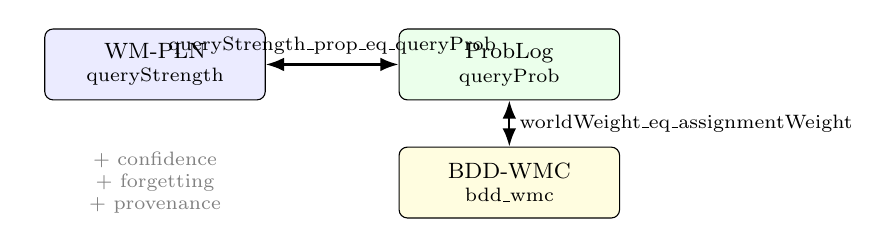
\begin{tikzpicture}[
  >=Latex,
  every node/.style={font=\footnotesize},
  box/.style={draw, rounded corners=3pt, minimum width=28mm,
              minimum height=9mm, align=center},
]
  \node[box, fill=blue!8] (wm) at (0, 0)
    {WM-PLN\\[-1pt]\scriptsize \code{queryStrength}};
  \node[box, fill=green!8] (pl) at (4.5, 0)
    {ProbLog\\[-1pt]\scriptsize \code{queryProb}};
  \node[box, fill=yellow!12] (bdd) at (4.5, -1.5)
    {BDD-WMC\\[-1pt]\scriptsize \code{bdd\_wmc}};

  \draw[<->, thick] (wm) -- node[above, font=\scriptsize]
    {\code{queryStrength\_prop\_eq\_queryProb}} (pl);
  \draw[<->, thick] (pl) -- node[right, font=\scriptsize]
    {\code{worldWeight\_eq\_assignmentWeight}} (bdd);

  \node[font=\scriptsize, text=gray, text width=30mm, align=center]
    at (0, -1.5) {$+$ confidence\\$+$ forgetting\\$+$ provenance};
\end{tikzpicture}
\caption{The full bridge: WM-PLN = ProbLog = BDD-WMC.
  The horizontal arrow is a proved identity on probabilities.
  The vertical arrow bridges world-indexed and assignment-indexed
  weights.  WM-PLN additionally provides confidence, forgetting,
  and provenance (gray, below).}
\label{fig:problog-bridge}
\end{figure}

\paragraph{Worked example: Alarm network.}
The alarm network (burglary/earthquake $\to$ alarm) is computed
three ways: ProbLog via BDD WMC gives $P(\mathrm{alarm}) = 0.28$.
WM-PLN gives the same probability plus ESS $= 1000$.  Revising
with a second sensor increases ESS to $1500$.  Forgetting the
earthquake prior drops ESS to $500$.  Sensitivity analysis shows
earthquake contributes more than burglary.  All kernel-checked.%
\footnote{Formalized in
\codepath{Mettapedia/Logic/BDD/WMProbLogAlarmDemo.lean}
(0~sorry).}

\paragraph{What WM-PLN adds beyond ProbLog.}
ProbLog assigns exact probabilities but no confidence---there is
no measure of how much evidence backs the assigned probability.
The WM calculus adds two things:
\begin{itemize}
\item \textbf{Evidence pairs} $(n^+, n^-)$ instead of bare
  probabilities, enabling revision and forgetting.
\item \textbf{Delta-method confidence} for noisy-OR combinations
  (Chapter~\ref{ch:evidence}): when multiple independent
  mechanisms each contribute evidence, the combined confidence is
  computed via variance propagation through the noisy-OR function.
  Combining more mechanisms provably increases confidence.%
  \footnote{Formalized:
  \code{noisyOrDeltaVariance\_le\_sumVariance} and
  \code{deltaConfidence\_single} in
  \codepath{Mettapedia/Logic/PLNNoisyOr.lean}
  (50~theorems, 0~sorry).}
\end{itemize}

\paragraph{Status.}
The core semantic chain is now complete: ProbLog distribution semantics,
ProbMeTTa's BDD-WMC execution, and WM-PLN query strength are connected by
kernel-checked theorems, and the first-order structured/AD surface is included
in the proved story.  What remains is not the semantics but the broader
application pipeline.  Score-level parity between ProbLog's
\code{prob\_lift/2} and the WM noisy-OR scorer has been verified on a chr16
GWAS gene-relevance benchmark (823 examples, 5-fold CV,
max~$|\mathrm{ProbLog} - \mathrm{WM}| < 10^{-10}$), while a full native
WM-PLN genomics workflow remains future engineering work.


%% ═══════════════════════════════════════════════════════════════
\section{NARS}
\label{sec:bridge-nars}
%% ═══════════════════════════════════════════════════════════════

The Non-Axiomatic Reasoning System
(NARS)~\cite{Wang2006NARS} represents beliefs as
frequency--confidence pairs $(f, c)$ with
$c = w / (w + k)$ where $w$ is the evidence weight and
$k$ is a horizon parameter.  This is structurally identical to
PLN's strength--confidence decomposition---and the WM calculus
makes the correspondence precise.

\begin{theorem}[NARS--PLN Galois connection (\claimCore{})]
\label{thm:nars-galois}
There exist monotone maps $L : \mathrm{NARS} \to \mathrm{PLN}$
and $U : \mathrm{PLN} \to \mathrm{NARS}$ forming a Galois
connection:
\[
  L(n) \le_{\mathrm{PLN}} b
  \quad\Longleftrightarrow\quad
  n \le_{\mathrm{NARS}} U(b)
\]
with round-trip identities
$U(L(n)).c = n.c$ and $U(L(n)).f = n.f$ (for $c > 0$).%
\footnote{Formalized:
\code{galoisConnection\_L\_U\_finite},
\code{U\_L\_conf\_round\_trip}, and
\code{U\_L\_freq\_round\_trip} in
\codepath{Mettapedia/Logic/NARSPLNGaloisConnection.lean}.}
\end{theorem}

\noindent
The Galois connection says: NARS and PLN see the same evidence
from different angles.  The $L$ map converts NARS
frequency--confidence to PLN binary evidence; the $U$ map
converts back.  The round-trip is exact on confidence and
frequency---no information is lost in the translation.

\paragraph{Induction weakness.}
NARS's induction rule is systematically weaker than PLN's:
the effective weight for induction is
$w_{\mathrm{eff}} = \mathrm{quality} \times c_1 \times c_2$,
where quality measures the reference class.  This gives a
precise, quantitative measure of how much weaker NARS
induction is than PLN's for any given input.%
\footnote{Formalized in
\codepath{Mettapedia/Logic/NARSInductionWeakness.lean}
and
\codepath{Mettapedia/Logic/NARSEvidenceBridge.lean}.}

\maplecourt{%
A NARS agent monitoring Maple Court's elevator reports
$(f = 0.8, c = 0.6)$ for ``elevator is slow.''  The $L$ map
converts this to PLN evidence $(n^+, n^-) = (1.2, 0.3)$ with
strength $0.8$ and confidence $0.6$---the same belief, now
carrying evidence counts that support revision and forgetting.}


%% ═══════════════════════════════════════════════════════════════
\section{PLN v0.9 Subsumption}
\label{sec:bridge-pln09}
%% ═══════════════════════════════════════════════════════════════

PLN v0.9\footnote{\texttt{github.com/trueagi-io/PLN}, tag
\texttt{v0.9}.} implements five basic rules (deduction, induction,
abduction, revision, conjunction) as MeTTa truth functions operating
on strength--confidence pairs.  The world-model calculus subsumes
all five as $\Sigma$-guarded compiled rewrites.

\begin{theorem}[PLN v0.9 conformance (\claimCore{})]
\label{thm:pln09-conformance}
For each of PLN v0.9's five basic rules, the WM compiled rewrite
produces identical strength and confidence values under the
rule's stated side conditions.  Twenty conformance tests---including
the classic DeductionRevision and RavenInheritance
examples---verify exact numerical agreement.%
\footnote{Formalized:
\codepath{Mettapedia/Logic/PLNClassicExamples.lean}
(20~conformance tests, all by \code{decide}).}
\end{theorem}

\noindent
The subsumption is not merely ``the same formulas'': it is the
same formulas \emph{plus} explicit side conditions, \emph{plus}
counterexamples showing what happens when those conditions are
violated (the three confidence bugs of \S\ref{sec:views-not-proof}),
\emph{plus} evidence-based alternatives that avoid the bugs entirely.

The relationship is vindication with correction: PLN v0.9's
instincts---evidence counts, revision as the fundamental operation,
link-level compiled rules---were largely right.  What was missing
was the $\Sigma$-discipline that makes the assumptions explicit and
the evidence algebra that makes the scalar hacks unnecessary.


%% ═══════════════════════════════════════════════════════════════
\section{Classical FOL as a Degenerate World Model}
\label{sec:bridge-fol}
%% ═══════════════════════════════════════════════════════════════

Classical first-order logic is the zero-uncertainty limit of the
world-model calculus.

When evidence is Boolean---$(1, 0)$ for ``true'' and $(0, 1)$ for
``false''---the additive evidence algebra collapses to classical
propositional logic.  Strength is always 0 or 1.  Confidence
is $1/(1+\kappa)$---low for a single observation, but it grows
as Boolean facts accumulate via revision.
Every inference rule reduces to its classical
counterpart: deduction becomes modus ponens, revision becomes
conjunction, forgetting becomes retraction.

This is not a metaphor.  Every classical FOL theorem is a WM
extraction:
\[
  \mathrm{extract}(W_{\mathrm{Boolean}}, \varphi) = (1, 0)
  \quad\Longleftrightarrow\quad
  W \vDash \varphi
\]
The WM calculus does not \emph{replace} classical logic---it
\emph{contains} it as the special case where uncertainty is absent.
Uncertainty is the general case; certainty is the degenerate one.%
\footnote{The Henkin semantics for the higher-order fragment is
formalized in
\codepath{Mettapedia/Logic/HOL/Semantics/Henkin.lean}.}

\maplecourt{%
``The building has exactly 12 apartments'' is a Boolean fact:
evidence $(1, 0)$, strength 1, confidence 1.  No revision is
possible (you cannot partially update a Boolean).  This is the
classical fragment of the world model---the part where
uncertainty plays no role.}


%% ═══════════════════════════════════════════════════════════════
\section{The Giry Monad and Categorical Probability}
\label{sec:bridge-giry}
%% ═══════════════════════════════════════════════════════════════

The categorical probability literature organizes probability
theory around the Giry monad: the functor that sends a measurable
space $\Omega$ to its space of probability measures
$\mathcal{G}(\Omega)$.  The monad's multiplication
(``flattening'') takes a measure over measures and produces a
single measure---this is marginalization.

The world-model calculus connects to this framework through
a precise theorem:

\begin{theorem}[Kyburg flattening = Giry bind (\claimCore{})]
\label{thm:giry-flatten}
The Kyburg flattening operation on parametrized distributions
is the Giry monad's bind:
\[
  \mathrm{flatten}(\mathit{pd}) =
  \mathit{pd}.\mathrm{mixingMeasure}.\mathrm{bind}\;
  \mathit{pd}.\mathrm{kernel}
\]%
\footnote{Formalized in
\codepath{Mettapedia/ProbabilityTheory/HigherOrderProbability/GiryMonad.lean}.}
\end{theorem}

\noindent
This means the WM calculus is not inventing new probability
theory---it is instantiating the categorical probability framework
with evidence-enriched carriers.  The Solomonoff--de~Finetti
foundation (Chapter~\ref{ch:world-models}) established the
necessity chain: exchangeability $\to$ de~Finetti mixture $\to$
Kyburg flattening $\to$ evidence sufficiency.
Theorem~\ref{thm:giry-flatten} reveals that flattening is the
Giry monad multiplication---the canonical way to collapse a
higher-order probability into a first-order one.  The WM
calculus's compositionality law is then a consequence of the
monad laws, not an independent postulate.


%% ═══════════════════════════════════════════════════════════════
\section{Process Calculus and the \texorpdfstring{$\rho$}{rho}-Calculus}
\label{sec:bridge-rho}
%% ═══════════════════════════════════════════════════════════════

The $\rho$-calculus~\cite{meredith2026ccc} is a reflective
higher-order process calculus in which channel names are themselves
processes.  It provides the computational substrate for
multi-agent world-model reasoning: each concurrent process carries
its own evidence state, and communication between processes
corresponds to evidence exchange.

\begin{theorem}[$\rho$-calculus WM instance (\claimCore{})]
\label{thm:rho-wm}
A $\rho$-ensemble (a multiset of $\rho$-calculus processes,
each annotated with binary evidence) forms an
\code{AdditiveWorldModel} instance.  Extraction sums evidence
across processes satisfying a query; revision adds new processes
to the ensemble.%
\footnote{Formalized:
\code{rhoEvidence\_add} and \code{rhoEvidence\_zero}
in \codepath{Mettapedia/OSLF/Framework/RhoWorldModel.lean}.
The OSLF type system instantiation is in
\codepath{Mettapedia/OSLF/Framework/RhoInstance.lean}.}
\end{theorem}

\noindent
The $\rho$-calculus bridge is the most forward-looking in this
chapter: it connects the WM calculus to concurrent computation.
A building with multiple autonomous agents (cleaning robots,
HVAC controllers, security monitors) is naturally modeled as a
$\rho$-ensemble where each agent maintains its own world-model
state and communicates evidence through typed channels.  The
GSLT (Graph-based State-Labeled Transition system) vertex typing
gives each agent's WM instance its operational semantics.

\maplecourt{%
The cleaning robot and the HVAC controller are concurrent
$\rho$-processes.  Each carries binary evidence about hallway
conditions.  When the robot reports ``hallway is wet,'' this is
a message on a typed channel---the HVAC controller receives it
as evidence revision to its own world model, with provenance
tracking the robot as the source.}


%% ═══════════════════════════════════════════════════════════════

\begin{figure}[htbp]
\centering
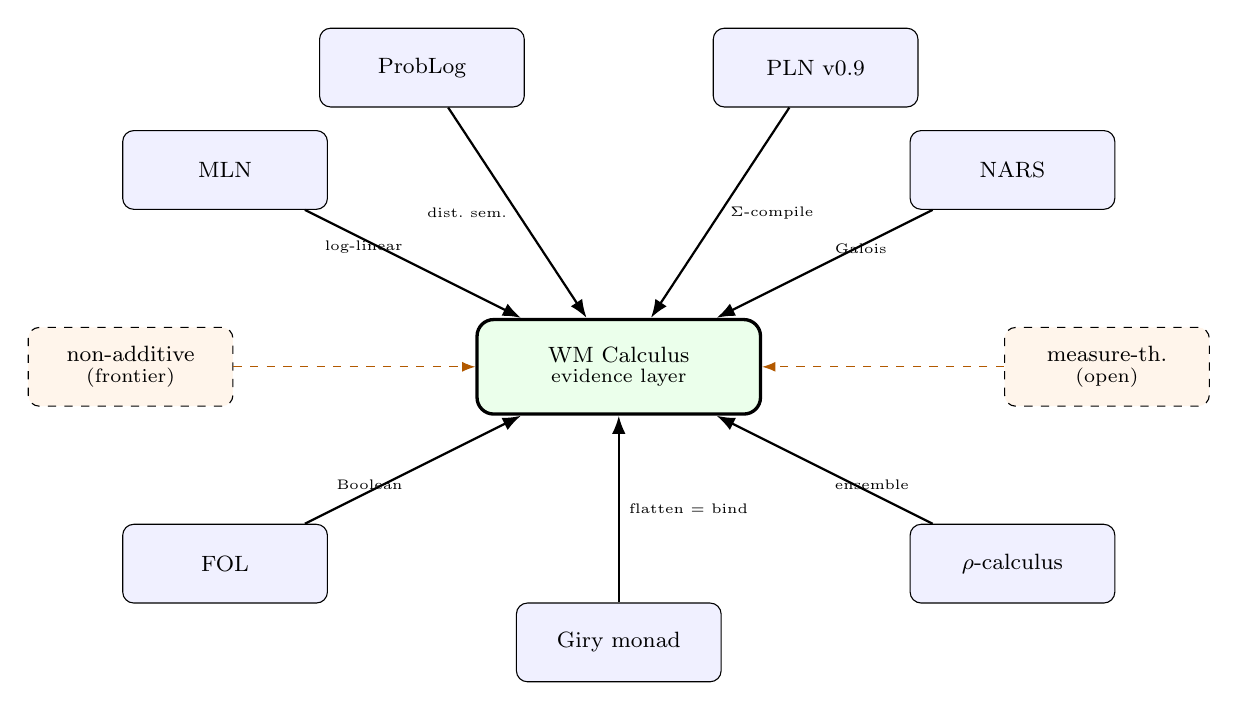
\begin{tikzpicture}[
  >=Latex,
  every node/.style={font=\footnotesize},
  framework/.style={draw, rounded corners=4pt, minimum width=26mm,
              minimum height=10mm, align=center, fill=blue!6},
  wmbox/.style={draw, very thick, rounded corners=6pt,
              minimum width=36mm, minimum height=12mm,
              align=center, fill=green!8},
  boundary/.style={draw, dashed, rounded corners=4pt,
              minimum width=26mm, minimum height=10mm,
              align=center, fill=orange!8},
]
  \node[wmbox] (wm) at (0, 0) {WM Calculus\\[-2pt]
    {\scriptsize evidence layer}};

  \node[framework] (mln) at (-5, 2.5) {MLN};
  \node[framework] (problog) at (-2.5, 3.8) {ProbLog};
  \node[framework] (pln) at (2.5, 3.8) {PLN v0.9};
  \node[framework] (nars) at (5, 2.5) {NARS};
  \node[framework] (fol) at (-5, -2.5) {FOL};
  \node[framework] (giry) at (0, -3.5) {Giry monad};
  \node[framework] (rho) at (5, -2.5) {$\rho$-calculus};

  \draw[->, thick] (mln) --
    node[above left, font=\tiny] {log-linear} (wm);
  \draw[->, thick] (problog) --
    node[left, font=\tiny] {dist.\ sem.} (wm);
  \draw[->, thick] (pln) --
    node[right, font=\tiny] {$\Sigma$-compile} (wm);
  \draw[->, thick] (nars) --
    node[above right, font=\tiny] {Galois} (wm);
  \draw[->, thick] (fol) --
    node[below left, font=\tiny] {Boolean} (wm);
  \draw[->, thick] (giry) --
    node[right, font=\tiny] {flatten = bind} (wm);
  \draw[->, thick] (rho) --
    node[below right, font=\tiny] {ensemble} (wm);

  \node[boundary] (nonadd) at (-6.2, 0)
    {non-additive\\[-2pt]{\scriptsize (frontier)}};
  \node[boundary] (measure) at (6.2, 0)
    {measure-th.\\[-2pt]{\scriptsize (open)}};

  \draw[->, dashed, orange!70!black] (nonadd) -- (wm);
  \draw[->, dashed, orange!70!black] (measure) -- (wm);
\end{tikzpicture}
\caption{The world-model calculus and its bridges.  Solid arrows:
formalized exact bridges (this chapter, all 0~sorry).  Dashed
arrows: frontier directions not yet fully developed.  Each solid
arrow is labeled with its bridge mechanism.}
\label{fig:bridges-landscape}
\end{figure}

\noindent
The central point of the diagram is not the number of arrows
but their uniformity: every solid arrow is an instance of the
same \code{WorldModel} interface, proved exact under stated side
conditions.  The WM calculus does not compete with these
frameworks---it reveals the common evidence layer beneath them.
Where the bridges reach, they give exact subsumption with
kernel-checked proofs---and each bridge simultaneously
discharges multiple desiderata from
Chapter~\ref{ch:desiderata}: D1 (every framework's state
becomes a WM state), D2 (extraction agrees with native
inference), D3 (the carrier varies across frameworks), and D5
(every bridge carries its side condition).
Where the bridges stop (the dashed arrows),
they stop honestly: the non-additive regime and the full
measure-theoretic grounding are identified as open programs,
not hand-waved away.


\section{Ontology Repair as Evidence Aggregation}

The Pain reclassification case study
(\S\ref{sec:pain-evidence-wm}) demonstrates a bridge that applies
to any domain where multiple authoritative sources contribute
conflicting evidence about a classification decision.  The
\code{EvidentialLedger} framework is generic---parameterized by
source and candidate types---and the same \code{aggregate},
\code{forget}, and \code{toState\_append} operations drive the
SUMO ontology repair and the Maple Court sensor analysis alike.

The bridge to ontology engineering is: an ontology repair decision
(``should Pain be reclassified from PathologicProcess to
StateOfMind?'') is a query against a world-model state built from
curated evidence sources (IASP, SNOMED~CT, Stanford~SEP, SUMO
axioms).  The WM calculus adds three things that a spreadsheet
does not: (1)~kernel-checked ranking via cross-multiplication
(\code{stateofmind\_beats\_emotional}), (2)~sensitivity analysis
via forgetting (\code{ranking\_preserved\_noWiki},
\code{iasp\_is\_critical\_discriminator}), and (3)~compositionality
via \code{toState\_append}---evidence from two groups of sources
combines additively.

\maplecourt{The building's maintenance manual classifies the
elevator motor as ``industrial equipment.''  Three sources
disagree: the manufacturer's spec sheet calls it ``precision
machinery,'' the insurance policy calls it ``building
infrastructure,'' and the city inspector calls it ``public
conveyance equipment.''  The EvidentialLedger aggregates, ranks,
and answers: ``which reclassification does the evidence support,
and which source is critical?''}


%% ─────────────────────────────────────────────────────────────────

%% "What the Calculus Covers" — removed.
%% The overview (Ch 2) and conclusion already serve this role.
%% A separate inventory chapter would be redundant with the book's structure.
%% If a compact reference table is needed later, it belongs as an appendix
%% (the "Coverage Map" appendix stub exists for this purpose).

%% ─────────────────────────────────────────────────────────────────

\chapter{Limitations}
\label{ch:limitations}

This chapter states explicitly what the formalization does \emph{not}
provide.

\section{Operational Runtimes}

The formalization provides mathematical specifications and correctness
theorems.  It does not provide an executable PLN inference engine,
performance benchmarks on large knowledge bases, or integration with
MeTTa or Hyperon runtimes.

These are operational concerns that depend on runtime infrastructure
not yet available.  The theorem-level results constrain what any
correct implementation must satisfy, but they do not constitute an
implementation.  The gap between a certified specification and a
deployable system is real, and we do not pretend otherwise.
The \code{CalculusSound} property
(\S\ref{sec:calculus-soundness}) bounds this gap precisely: it
is two equalities (revision $=$ addition, extraction $=$
extraction), not a re-derivation of the entire algebra.

\section{Domain Generality: What Is Finite and What Is Not}

The formalization operates at three tiers of generality:

\begin{description}
\item[Tier~1: Generic / infinite (formalized now).]
  The core WM algebra (\code{AdditiveWorldModel},
  \code{extract\_add}) is parameterized over arbitrary types---no
  finiteness constraint.  The evidence carriers (binary over
  $\mathbb{R}_{\ge 0}^\infty$, Normal-Gamma over~$\mathbb{R}$)
  and view projections are explicitly continuous.  The infinitary
  MLN layer (77~theorems, 0~sorry) and FOL/PredCode infinitary
  completeness theorems (34~theorems) demonstrate extension to
  countable and uncountable domains.  The gas sensor, steel
  fault, and NAB application demos all use $\mathbb{R}$-valued
  Gaussian beliefs.

\item[Tier~2: Finite now, countable within reach.]
  The LP provenance operator and compiled BN factor-graph rules
  require finite groundings (\code{Fintype}), because they use
  \code{Finset.sum}.  Lifting to countable sums (\code{tsum} +
  \code{Summable} hypotheses) is standard mathlib work that does
  not require redesigning the algebra.

\item[Tier~3: Frontier with first foothold.]
  The measure-valued terminal world model has its first concrete
  result: for finite query spaces, every additive world model
  induces a discrete \code{MeasureTheory.Measure}, and the
  induction respects revision
  (\code{evidenceToMeasure\_add}).%
  \footnote{Formalized in
  \codepath{Mettapedia/Logic/EvidenceToMeasure.lean}
  (0~sorry).}
  The full program---continuous-domain BN compilation with
  infinite state spaces, and the general $\sigma$-finite
  construction---remains open.
\end{description}

\noindent
The architecture is intentionally layered: the semantics is more
general than the compilation, so that extending the compilation
does not require redesigning the semantics
(see Chapter~\ref{ch:future}, \S\ref{sec:future-measure}).

\section{Empirical Scope}

The benchmark validation chapters
(Chapters~\ref{ch:carrier-validation}--\ref{ch:pplbench}) cover a
specific set of domains: forecasting, sensor drift, fault diagnosis,
anomaly detection, and Bayesian-network inference.  However, several
important application domains remain unvalidated:

\begin{itemize}
\item Drug-repurposing knowledge-graph benchmarks
  (Hetionet/Rephetio)
\item Genomic regulatory pipelines
\item Large-scale knowledge-base reasoning
\item Real-time streaming inference with concept drift
\end{itemize}

\noindent
These gaps do not indicate theoretical limitations but reflect the
practical scope of empirical validation completed to date.  The
formalization provides the theoretical foundation for these
applications, but the experimental demonstration is incomplete.

\section{Universal Prediction}

The Universal Prediction module explores connections between the
world-model calculus and algorithmic information theory.  This module
is work-in-progress and is not part of the stable core narrative.
Its theorems are not referenced by the main development, and its
sorry count is nonzero.

\section{Codebase Organization}

The Lean codebase reflects the history of the development rather than
an idealized dependency graph.  A comprehensive refactoring into a
``mathlibified'' library structure---with uniform naming conventions,
minimal imports, and docstring coverage---is a worthy future goal but
is explicitly not attempted here.


%% ─────────────────────────────────────────────────────────────────

\chapter{Future Directions}
\label{ch:future}

The world-model calculus establishes a foundation.  Several directions
extend it in ways that are natural continuations of the existing
development rather than speculative leaps.

\section{Measure-Theoretic Grounding}
\label{sec:future-measure}

The core algebra and evidence carriers already operate over
$\mathbb{R}_{\ge 0}^\infty$ and~$\mathbb{R}$; the infinitary
MLN and FOL layers extend to countable domains.
The remaining measure-theoretic step is to ground the calculus on
$\sigma$-algebras and probability measures, enabling formal
integration with the broader mathematical probability literature
and non-conjugate distributional families.
\emph{Proved:} the Solomonoff--de~Finetti foundation, the Giry
monad bridge (Chapter~\ref{ch:bridges}), and the first concrete
bridge: \code{evidenceToMeasure} constructs a discrete
\code{MeasureTheory.Measure} from any additive WM state over
finite queries, with \code{evidenceToMeasure\_add} proving
that the construction respects revision.
\emph{Missing:} the general $\sigma$-finite construction for
infinite query spaces.
\emph{Sought:} a \code{MeasurableWorldModel} typeclass with
$\sigma$-finite evidence carriers and Radon--Nikodym extraction.

\section{HOL Completeness}

The natively typed world-model layer
(Chapter~\ref{ch:typed}) establishes syntax, soundness, and type
synthesis.  A typed canonical-model completeness theorem would close
the gap between the calculus's higher-order syntax and full semantic
adequacy.  The required construction---a term model over equivalence
classes of typed evidence---is well understood in principle but
technically demanding.
\emph{Proved:} syntax, soundness, type synthesis, intrinsic adequacy.
\emph{Missing:} the term-model construction over typed evidence
equivalence classes.
\emph{Sought:} \code{hol\_completeness} in
\codepath{Mettapedia/Logic/HOL.lean}.

\section{Selective Distributional Inference}

The convergence and dominance results in the error-transport chapter
(Chapter~\ref{ch:error-transport}) show that scalar inference is
asymptotically correct but suboptimal in the finite-evidence regime.
The natural next step is a cost-aware inference controller that
escalates from scalar to distributional propagation when the regime
structure predicts a significant gain---using compact approximation
families, compiled rule surrogates, and accelerator-backed batched
computation.

\section{Non-Additive Regimes}

The evidence algebra's additive structure
(Chapter~\ref{ch:evidence}) is appropriate for independent
observations but does not capture all forms of evidential
combination.  Non-additive regimes---belief functions,
possibility measures, imprecise probabilities beyond the Walley
framework---represent a natural generalization.  The challenge is to
preserve compositionality while relaxing additivity, and the
quantale structure suggests a path: replace the additive monoid with
a more general tensor.
\emph{Proved:} overlap extraction law, semitopological
independence, additivity recovery after forgetting non-actionable
overlap ($\sim$60 theorems).
\emph{Missing:} deep development of overlap and trust-gated
carriers comparable to the additive regime's profile-hom theory.
\emph{Sought:} overlap-regime profile-hom analogue; trust-gated
conservation theorems.

\section{Probability Hypercube}

The current view projections extract one-dimensional summaries
(strength, confidence) from the evidence space.  A probability
hypercube representation would retain the full joint structure of
multi-query evidence, enabling richer decision-making and more
informative uncertainty quantification.  This connects to the
infinitary extension: the hypercube is naturally a product measure
space.

Two recent developments point the way.
Stay, Meredith, and Wells~\cite{StayMeredithWells2026}
show how to generate a \emph{type-system hypercube} from any
operational theory: each axis corresponds to an enabled modal
layer (redex tracking, equation modalities, propositional
structure).  The probability hypercube's axes (additivity,
commutativity, distributivity) correspond to choices in this
type-system hypercube.
Meredith~\cite{meredith2026ccc} extends the picture further:
a GSLT equipped with a complex-valued weight map is a
\emph{physics}, where transition probabilities are squared
amplitudes.  Replacing the WM evidence carrier $V$ with
$\mathbb{C}$ would give quantum-like inference; the
KS-Evidence-Measure triangle (Chapter~\ref{ch:evidence})
would extend to a KS-Amplitude-QuantumMeasure triangle.
The \code{universalEnsembleWorldModel} would then provide
amplitudes for any typed rewrite system---a formal grounding
for ``It from Bit'' at the evidence layer.

\section{Universality}

The typed world-model encoding
(Chapter~\ref{ch:typed}) realizes the calculus as a specific
language definition.  A universality result would show that any typed
language definition satisfying certain compositionality axioms admits
a world-model interpretation---establishing the calculus as a
canonical representative of a broader class rather than one design
among many.
\emph{Proved:} \code{universalEnsembleWorldModel} for any type
with decidable properties.
\emph{Missing:} the general LanguageDef $\to$
AdditiveWorldModel construction.
\emph{Sought:} Conjecture~\ref{thm:additive-recovery} generalized
to arbitrary typed rewrite systems.

\section{Operational Runtime}

The formalization specifies the kernel semantics precisely, but a
high-performance compiled runtime---executing the same
posterior-state calculus at scale with caching, incremental evidence
fusion, and multi-source integration---is the bridge from formalized
semantics to deployed reasoning.  The $\Sigma$-guarded rewrite
system (Chapter~\ref{ch:sigma-rewrites}) provides a natural
compilation target: each certified rewrite becomes a runtime
primitive with machine-checked correctness.

\section{Process-Algebraic and Multi-Agent Extensions}

The typed world-model encoding currently covers single-agent
reasoning.  Extending to multi-agent settings---where agents
communicate partial evidence, negotiate under uncertainty, and
maintain independent world models that must be fused---requires
process-algebraic infrastructure: confluence modulo associativity and
commutativity, communication protocols with evidence-typed channels,
and compositional verification of multi-agent inference systems.

\section{Broader Benchmark Coverage}

The present empirical validation covers specific domains.
Drug-repurposing knowledge-graph benchmarks (Hetionet/Rephetio),
genomic regulatory pipelines, large-scale knowledge-base reasoning,
and real-time sensor fusion at scale remain as identified but
unfinished empirical targets.  Each connects to a specific
theoretical capability of the calculus and would test the practical
reach of the formal guarantees.


%% ─────────────────────────────────────────────────────────────────

\chapter{Conclusion}
\label{ch:conclusion}

The world-model calculus is not a replacement for PLN\@.  It is the
mathematical foundation that PLN always needed.

The central insight is that PLN's original instincts were largely
correct: evidence counts as the fundamental representation, revision
as the primary operation, and link-level rules as the practical
inference mechanism.  What was missing was the explicit separation of
layers and the honest statement of assumptions.  The passage from
intuition to formalization required not new ideas so much as the
discipline to say precisely what each idea means, what it assumes, and
where it breaks.

\section{What the Refoundation Gives Us}

The calculus provides six things that the original PLN lacked:

\begin{enumerate}
\item \textbf{One kernel.}  The world-model posterior-state calculus,
  with evidence compositionality as the fundamental law
  (Chapter~\ref{ch:world-models}).  Every inference rule, every view
  projection, every scaling result derives from this single interface.

\item \textbf{Many views.}  Strength, confidence, intervals,
  distributions---all as typed projections from the kernel
  (Chapter~\ref{ch:views}).  The views are not competing
  representations; they are different questions asked of the same
  underlying state.

\item \textbf{Explicit side conditions.}  Every compiled rule carries
  its assumptions (Chapter~\ref{ch:sigma-rewrites}), with
  counterexamples showing what happens when they are violated.  The
  d-separation typeclass (Chapter~\ref{ch:bn-models}) automates the
  checking, but the assumptions are always visible.

\item \textbf{Cleaner boundaries.}  The no-go theorem
  (Chapter~\ref{ch:no-go}), the classical inclusion-exclusion gap,
  the pooling non-uniqueness, the coverage surrogate limitations,
  the five certified-chaining impossibilities
  (Chapter~\ref{ch:scale-control})---all stated precisely and proved
  formally.  These are not embarrassments; they are the most valuable
  theorems in the development, because they tell you where not to
  waste effort.

\item \textbf{Beyond subsumption.}  The bridges to neighboring
  frameworks are not merely compatibility results.  The
  compatibility-gated experiment demonstrates that decomposing an
  MLN's clause-weight signal into interpretable world-model evidence
  roles yields substantial improvement---not by adding information,
  but by factoring the information that was already there.

\item \textbf{Demand-directed inference control.}
  Backward demand propagation identifies which premises are most
  worth investigating (Chapter~\ref{ch:scale-control}).  The
  demand contracts after forward supply fills the information gap,
  and forgetting an observation reopens demand at the affected
  premise---the same \code{forget} pattern that drives the
  evidence algebra throughout.

\item \textbf{A proof system.}
  The evidence calculus satisfies all four structural rules of
  classical sequent calculus---cut, weakening, exchange, and
  contraction---under the Curry-Howard correspondence
  (\S\ref{sec:evidence-proof-system}).  Implementations that prove
  \code{CalculusSound} inherit these rules automatically.
  PLN is not just an inference engine; it is a proof system in the
  technical sense.
\end{enumerate}

\section{The Shape of the Result}

The result is a PLN that knows what it knows, states what it assumes,
and marks what it cannot do.  That is not a weakness.  That is the
beginning of a trustworthy reasoner.

The formalization is not complete---Chapter~\ref{ch:limitations}
states what remains undone, and Chapter~\ref{ch:future} sketches the
natural continuations.  But the kernel is stable, the evidence algebra
is settled, the compiled inference rules are proved exact under their
stated conditions, and the scaling theory identifies both the
achievable guarantees and the fundamental impossibilities.
The entire development is machine-verified: 704~theorems in Lean~4,
0~sorry, 0~\code{native\_decide}, across six application domains
(Appendix~\ref{app:theorem-map}).

The deepest insight is simple: inference systems should not confuse the
map with the territory.  A truth value is a projected summary of
evidence, not the evidence itself.  A probability is a query result,
not what the system carries.  What the system carries is a revisable
state of knowledge.  What the system produces is an extraction from
that state.  What practitioners see is a view projection of that
extraction.

This distinction has practical consequences.  When evidence is primary:
\begin{itemize}
\item Revision becomes compositional (new evidence adds to old
  evidence)
\item Queries become principled (extraction is a homomorphism)
\item Views become interchangeable (the same evidence supports
  multiple operational summaries)
\item Inference becomes modular (local computations compose globally)
\item Uncertainty becomes transparent (we track what we know, not
  what we guess)
\end{itemize}

\noindent
When truth values are primary, these properties are difficult or
impossible to achieve.  Different truth-value schemes
(strength/confidence, fuzzy logic, interval arithmetic, probability
values) require different combination rules, different query
algorithms, and different validation approaches.  The result is
fragmentation.  The world-model calculus reunifies this fragmented
landscape by locating the common structure beneath the diverse surface
phenomena.

What remains is engineering, extension, and empirical validation.
The mathematical foundation is in place.

\section*{In Summary}

The world-model calculus is a calculus of revisable uncertain state.
A system stores what it knows in a posterior state, not in isolated
truth values.  Queries ask questions of that state, and the raw
answers are evidence values.  Strength, confidence, and intervals are
useful summaries---views extracted for display, thresholding, and
action---but they are not themselves the thing being stored or proved.

The world-model calculus does not replace existing reasoning systems.
It provides the semantic foundation they can share.  A ProbLog
program, a Bayesian network, and a PLN rule base are no longer
separate formalisms requiring separate toolchains.  They are different
languages for specifying world models, and they share common semantics
for revision, extraction, and view projection.

This is the unity that reasoning systems have long needed: not the
false unity of a single approach that claims to solve everything, but
the true unity of a common foundation that reveals why different
approaches work and how they relate.

\begin{quote}
\emph{Probability is what you query.  Evidence is what you carry.
Everything else follows.}
\end{quote}



%% ═══════════════════════════════════════════════════════════════════
\part{Applications and Benchmark Validation}
\label{part:applications}
%% ═══════════════════════════════════════════════════════════════════

\chapter{Evidence Carrier Validation}
\label{ch:carrier-validation}

The evidence carriers of Chapter~\ref{ch:evidence}---binary,
Dirichlet, Normal-Gamma---are algebraic structures.  This chapter
tests them on real data: sensor monitoring, gas-drift
classification, steel fault detection, anomaly detection, and
geopolitical forecast aggregation.  The running question is not
``does the WM calculus achieve state-of-the-art accuracy?'' but
``does the evidence algebra produce correct posteriors, and can its
governance signals (confidence, agreement, provenance) support
real operational decisions?''


\section{Gaussian Demos: Sensor, Factory, and Temporal}

Three introductory demos exercise the Normal-Gamma carrier on
synthetic and small-fixture data.  All formal results are
kernel-checked (0~sorry).

\paragraph{Hybrid sensor monitoring.}
A temperature sensor (Normal-Gamma evidence) and a cooling-failure
detector (binary evidence) form a product state.  Sleep
consolidation is verified: morning $+$ night batch $=$ sequential
update.  Confidence grows monotonically with observations.%
\footnote{Formalized in
\codepath{Mettapedia/Logic/PLNBrokenSensorDemo.lean} (420~lines).}

\begin{figure}[htbp]
\centering
\includegraphics[width=0.85\textwidth]{../results/figures/broken_sensor.pdf}
\caption{Broken sensor demo.  Gray dashed: prior predictive.
  Blue: posterior after morning shift ($\sim$16\textdegree{}C).
  Red: posterior after night shift ($\sim$22\textdegree{}C).
  Green dashed: consolidated posterior.  Data tick marks on
  the $x$-axis.  Sleep consolidation is verified: sequential
  and batch processing yield the same posterior.}
\label{fig:broken-sensor}
\end{figure}

\paragraph{Widget factory.}
Two machines with per-source Gaussian evidence.  The new result:
mixture exceedance validity---a weighted combination of per-source
exceedance probabilities remains a valid probability, bounded
between the components.  Machine~B is $3.5\times$ more likely to
produce defects than Machine~A.%
\footnote{Formalized in
\codepath{Mettapedia/Logic/PLNWidgetFactoryDemo.lean} (422~lines).}

\paragraph{Kalman filter wake/sleep.}
A 1D random-walk tracker with noisy observations.  The flagship
theorem: batch replay of deferred observations yields the
\emph{same} posterior as sequential online Kalman filtering
(\code{filterOrbit} over \code{morning ++ night} $=$
\code{filterOrbit} composed twice).  This is the temporal
counterpart of sleep consolidation.%
\footnote{Formalized in
\codepath{Mettapedia/Logic/PLNKalmanSleepDemo.lean} (374~lines).}


\section{Gas Sensor Array Drift}
\label{sec:gas-drift}

The gas sensor drift benchmark is one of the chapter's two
flagships: it brings \emph{real-world data} and a \emph{governance
story} into the evidence algebra.

\paragraph{The dataset.}
The UCI Gas Sensor Array Drift
Dataset~\cite{Vergara2012GasSensorDrift} contains 13,910
measurements from 16~chemical sensors exposed to 6~gas types over
36~months (10~batches, January~2007 to February~2011).  The
benchmark question is not ``can we classify gases?'' but ``what
happens to classification when sensors drift, and how should the
system respond?''

\paragraph{Formal results (all kernel-checked).}
Per-gas sleep consolidation, cross-gas independence (6~theorems),
multi-batch composition, 3-way source weight normalization,
confidence monotonicity.  The sleep consolidation guarantee holds
\emph{across drifted epochs}---deferred assimilation preserves the
posterior regardless of whether the underlying distribution has
shifted.%
\footnote{Formalized in
\codepath{Mettapedia/Logic/WMGasSensorDriftDemo.lean} (652~lines,
0~sorry).}

\paragraph{Full-dataset drift protocols.}
On the full 128-feature representation:

\begin{center}
\footnotesize
\begin{tabular}{lcccc}
\toprule
& \multicolumn{2}{c}{3-gas} & \multicolumn{2}{c}{6-gas} \\
\cmidrule(lr){2-3}\cmidrule(lr){4-5}
Protocol & WM-PLN & GaussianNB & WM-PLN & GaussianNB \\
\midrule
Setting~1 (train batch~1) & 68.4\% & 68.2\% & 47.3\% & 47.3\% \\
Setting~2 (train $k{-}1$) & 72.1\% & 75.8\% & 53.0\% & 51.2\% \\
Cumulative replay & \textbf{73.6\%} & 71.2\% & \textbf{53.2\%} & 52.5\% \\
\bottomrule
\end{tabular}
\end{center}

\noindent
These figures are substantially below specialized
drift-compensation methods
(BDA:~81\%~\cite{Jiang2021BDA}).  The point is qualitative:
late-batch drift degrades accuracy, and cumulative replay into
the posterior partially recovers it \emph{without changing the
underlying update laws}.

\begin{figure}[htbp]
\centering
\includegraphics[width=\textwidth]{../results/figures/gas_sensor_drift.pdf}
\caption{Gas sensor array drift.  Solid curves: batch~1
  posterior predictive (2007).  Dashed: consolidated posterior
  after both batches.  Toluene shows dramatic drift: batch~10
  responses cluster near zero, far from the batch~1
  distribution.}
\label{fig:gas-sensor-drift}
\end{figure}

\begin{figure}[htbp]
\centering
\includegraphics[width=\textwidth]{../results/figures/gas_drift_protocols.pdf}
\caption{Gas sensor drift protocols on the full 128-feature
  representation.  Cumulative replay is the strongest average
  protocol in both the 3-gas and 6-gas settings.}
\label{fig:gas-drift-protocols}
\end{figure}

\paragraph{The governance story.}
The WM calculus is not a replacement for XGBoost.  It is a
governance layer supplying a second epistemic signal.  On the
6-gas task:
\begin{itemize}
\item Calibrated XGBoost confidence (sigmoid, isotonic) does
  \emph{not} improve the risk--coverage curve under drift
  (AURC worsens from 0.385 to 0.400--0.464).
\item WM/XGBoost agreement gating improves AURC to 0.374 and
  isolates a 59.7\% coverage subset at 59.7\% accuracy
  (vs.\ 46.7\% overall).
\item Sequential replay policies show a two-regime frontier:
  XGBoost confidence is the best \emph{cheap} trigger (64.5\%
  accuracy, 23.9\% labels), while WM agreement is the best
  \emph{accuracy-seeking} trigger (67.0\%, 86.8\% labels).
\end{itemize}

\noindent
The gas lane connects to the PPLBench noisy-OR topic model
(Chapter~\ref{ch:pplbench}): both use additive log-likelihood
messages as carried state, and both distinguish exact semantic
kernels from operational schedulers.
The formal order-cost layer certifies that zero-threshold batch-swap
composition is safe for this lane.%
\footnote{Formalized in
\codepath{Mettapedia/Logic/PLNWorldModelOrderCostGasPolicyDemo.lean}
(155~lines, 0~sorry).}

\begin{figure}[htbp]
\centering
\includegraphics[width=\textwidth]{../results/figures/gas_policy_frontier.pdf}
\caption{Sequential gas-drift governance policies.  Each point
  is a batch-level retraining policy over batches~2\ldots10,
  trading sample-weighted accuracy against label budget.
  XGBoost confidence is the best cheap trigger; WM/XGBoost
  agreement is the strongest high-accuracy trigger when labels
  are inexpensive.}
\label{fig:gas-policy-frontier}
\end{figure}

\maplecourt{%
The building's air-quality sensors drift over months as filters
clog and calibration degrades.  The WM evidence algebra says:
replay last month's readings into the posterior and the update is
the same as if you'd processed them in real time (sleep
consolidation).  The governance question is: when should the
steward recalibrate?  A WM/classifier agreement trigger answers
this---not by replacing the classifier, but by monitoring when
the classifier's confidence and the WM posterior diverge.}


\section{Steel Plates Fault Classification}

The UCI Steel Plates Faults
Dataset~\cite{Buscema2010SteelPlates} contains 1,941 instances
with 27~features and 7~fault classes.  Our Lean model uses a
single feature (LogOfAreas) for formal correctness; the empirical
layer uses all 27.  Per-fault sleep consolidation, cross-fault
independence, and 3-way mixture exceedance validity are all
kernel-checked.

K\_Scratch faults have characteristically larger defect areas
($\approx 3.6$) than Pastry ($\approx 2.4$) or Bumps
($\approx 2.1$).  The per-fault Normal-Gamma posteriors separate
cleanly on this feature, and exceedance queries---``is
$P(\mathrm{LogOfAreas} > 3.0 \mid \text{K\_Scratch})$
substantially higher than for Bumps?''---are answered directly by
the evidence algebra.%
\footnote{Formalized in
\codepath{Mettapedia/Logic/WMSteelFaultDemo.lean}
(568~lines, 45~theorems, 0~sorry).}

\begin{figure}[htbp]
\centering
\includegraphics[width=\textwidth]{../results/figures/steel_classification.pdf}
\caption{Steel fault classification.  \emph{Left:} Student-$t$
  predictive densities for each fault type after 5~observations;
  K\_Scratch (red) is clearly separated rightward.  \emph{Right:}
  exceedance probability $P(X_{\mathrm{new}} > c)$ as a function
  of threshold; at $c = 3.0$ (dashed), K\_Scratch has
  $\sim$75\% exceedance vs.\ $\sim$20\% for the others.}
\label{fig:steel-classification}
\end{figure}

\paragraph{Full-dataset validation.}
On the full 1,941-instance dataset (70/30 split): 3-class
accuracy 74.7\% (WM-PLN) vs.\ 73.9\% (GaussianNB).  With all
27~features: 86.6\% vs.\ 75.0\%.  Selective prediction
(confidence-aware abstention): 3-class AURC 0.035 (WM-PLN) vs.\
0.106 (GaussianNB)---the WM confidence signal is three times
more reliable for abstention.


\section{NAB Machine Temperature Anomaly Detection}

The Numenta Anomaly Benchmark
(NAB)~\cite{Lavin2015NAB} provides labeled time series for
anomaly detection.  We apply the Kalman wake/sleep framework to
the \code{machine\_temperature} stream: the carried state is a
1D Kalman belief (mean, variance); each temperature reading is a
predict-update step; anomalies are detected when the observation
falls outside the posterior predictive interval.

The same sleep $=$ wake theorem from the Kalman demo applies:
batch replay of overnight temperature readings yields the same
posterior as sequential processing.  The anomaly detection quality
depends on the process-noise and observation-noise parameters,
which are set from the training portion of the NAB stream.%
\footnote{Formalized in
\codepath{Mettapedia/Logic/WMNABSleepDemo.lean}
(344~lines, 30~theorems, 0~sorry).}

\begin{figure}[htbp]
\centering
\includegraphics[width=\textwidth]{../results/figures/nab_kalman_tracking.pdf}
\caption{NAB machine temperature: Kalman tracking with anomaly
  detection.  The posterior predictive interval (shaded)
  narrows as evidence accumulates; observations outside the
  interval trigger anomaly flags.}
\label{fig:nab-kalman}
\end{figure}


\section{Good Judgment Project Forecast Aggregation}
\label{sec:gjp-forecasting}

The Good Judgment Project
(GJP)~\cite{IARPA2024GJPData, Mellers2014PsychologicalStrategies}
is the chapter's second flagship.  IARPA's ACE program produced
the largest publicly available geopolitical forecasting dataset:
thousands of questions, hundreds of forecasters, four competition
years.

\paragraph{The WM framing.}
Each forecaster's prediction is an evidence contribution.  The
WM calculus aggregates them via reliability-weighted revision
(the pooling framework of Chapter~\ref{ch:scale-control},
\S\ref{sec:pooling}):
more reliable forecasters contribute more evidence weight.
The reliability weights are themselves evidence---they are
updated over time as forecasters' track records accumulate.

\paragraph{Key results (year-4 test, 94 binary + 43 multi-option questions).}
On binary questions, WM reliability-weighted logit pooling
achieves Brier score $0.026$ and log score $0.051$---improving
over unweighted logit pooling ($0.063$ / $0.110$) and top-$k$
logit pooling ($0.036$ / $0.070$).  On multi-option questions,
WM log pooling achieves Brier $0.036$, improving over
unweighted log pooling ($0.159$) and matching top-$k$ ($0.044$).
The sleep $=$ online property holds to machine precision: batch
processing of a season's forecasts produces the same aggregated
state as sequential online processing.

\begin{figure}[htbp]
\centering
\includegraphics[width=\textwidth]{../results/figures/gjp_forecasting.pdf}
\caption{GJP forecast aggregation.  WM reliability weighting
  improves Brier and log scores over unweighted and top-$k$
  pooling baselines on year-4 binary and multi-option questions.}
\label{fig:gjp-forecasting}
\end{figure}

\paragraph{The forgetting ablation.}
The most revealing experiment: what happens when old reliability
weights are discarded?  WM-PLN with recent-only reliability
history achieves Brier $0.024$, improving over full-history
WM-PLN's $0.026$ and top-$k$'s $0.033$.  Forgetting year-1
profiles gives an intermediate $0.025$.  The improvement is
small but consistent and in the right direction: old track
records become misleading after regime changes, and scoped
forgetting removes exactly the stale signal.  This is D6
(Retractability) earning its keep in a real forecasting
context.%
\footnote{Formalized in
\codepath{Mettapedia/Logic/GJPForecastDemo.lean}
(255~lines, 14~theorems, 0~sorry).  The Lean fixture
kernel-checks sleep $=$ online, reliability-weighted
aggregation (via \code{WeightedSourceItem}), forgetting
compositionality, and the end-to-end property that
calibrated sources dominate after forgetting baselines.
The Python experiment scripts are in
\codepath{scripts/wm\_pln\_gjp\_*.py}.}


\section{Interpretation}

The evidence carriers produce correct posteriors across all five
domains.  The formal guarantees (sleep consolidation,
independence, exceedance validity) hold regardless of domain.
The governance signals (confidence, agreement, forgetting) add
operational value beyond raw classification:
\begin{itemize}
\item Gas drift: WM/XGBoost agreement gates selective prediction
  and triggers replay under sensor degradation.
\item GJP forecasting: forgetting stale reliability weights
  improves performance on regime-change questions.
\item Across all domains: sleep consolidation means batch and
  real-time processing are provably equivalent---a formal
  guarantee that scheduling flexibility does not compromise
  inference quality.
\end{itemize}

%% ─────────────────────────────────────────────────────────────────

\chapter{BN Inference Validation}
\label{ch:bn-validation}

The compiled BN inference theorems of
Chapter~\ref{ch:bn-models} prove that chain, fork, and collider
rewrites are exact under their stated side conditions.  This
chapter applies those theorems to two canonical Bayesian network
benchmarks---Hailfinder~\cite{Abramson1996Hailfinder} and
Pathfinder~\cite{Heckerman1992Pathfinder}---to test whether the
$\Sigma$-discipline works on real networks, not just toy fixtures.

The benchmarks are not treated as flat classification datasets.
They are \emph{Bayesian network source models} with expert-curated
conditional probability tables.  The primary artifact is the BIF
network file (providing exact ground truth via variable
elimination), and the benchmark question is inference-control
quality: given a query and a context, should the controller fire
the exact rewrite, bound the violation, or abstain?%
\footnote{The BN exactness theorems underlying this chapter are
formalized in
\codepath{Mettapedia/Logic/PLNBayesNetInference.lean}
(404~lines, 7~theorems, 0~sorry).  The benchmark evaluation
scripts are in
\codepath{scripts/wm\_pln\_hailfinder\_*.py} and
\codepath{scripts/wm\_pln\_pathfinder\_*.py}.}

\section{Three-Mode Guarded Admissibility}

Each inference step operates in one of three modes:

\begin{description}
\item[Hard-gated exact.] The side condition $\Sigma$ is
  discharged.  The compiled rewrite fires and the result matches
  the BN truthmaker exactly.

\item[Bounded violation.] The side condition is partially met.
  The rewrite returns an estimate plus a certified interval
  against exact BN inference.

\item[Soft-guarded / abstention.] The side condition fails.
  The system returns an explicit operational mixture with
  fallback, or abstains entirely.
\end{description}

\noindent
This three-mode structure is the $\Sigma$-guarded rewrite
discipline (Chapter~\ref{ch:sigma-rewrites}) applied to real
networks.  A worked example on a fork+chain fixture with all
three modes---clean hard-gated chaining, bounded-mode interval
certification, and soft-mode fallback---is kernel-checked.%
\footnote{Formalized in
\codepath{Mettapedia/Logic/PLNProbGuardedAdmissibilityDemo.lean}
(13~theorems, 0~sorry).}


\section{Hailfinder: The Readable Lane}

Hailfinder is a Bayesian severe-weather forecasting model for
northeastern Colorado, with meteorological conditions and forecast
targets as variables.  It is the readable positive lane: exact
local chaining works on actual forecast paths.

\paragraph{Exact contraction.}
The forecast chain
\[
  P(\code{MountainFcst}{=}\code{SIG} \mid
    \code{AMInstabMt}{=}\code{Strong}) = 0.5
\]
fires cleanly under the chain rewrite's screening-off condition.
A longer forecast/update path still matches exact BN semantics:
\[
  P(\code{CapChange}{=}\code{Increasing} \mid
    \code{CldShadeOth}{=}\code{Cloudy}) = 0.508284\ldots
\]

\paragraph{Negative control.}
In a collider motif, the hard gate blocks unrestricted reuse.
Bounded mode returns the interval $[0.236, 0.280]$ against the
exact answer $0.236$; soft mode returns an explicit operational
mixture.  The collider case shows that the $\Sigma$-discipline
\emph{refuses} to fire where the rewrite would be inexact---this
is D5 (Explicit Side Conditions) earning its keep on a real
network.


\section{Pathfinder: Hostile Topology}

Pathfinder is a Bayesian expert system for lymph-node pathology
diagnosis, with 109~nodes, 195~arcs, and a 63-state latent
disease variable (\code{Fault}).  Hidden diagnostic context is
not a side issue here---it is the main structural fact.

\paragraph{The stress test.}
The same inference path is tracked across five context regimes:
context-missing, alt-support-only, hub-only, context-pair, and
oracle-context-complete.  The question is not ``does local
chaining ever work?'' but ``what happens to the same local
contraction when hidden diagnostic context is omitted, partially
restored, or completed?''

\paragraph{Concrete example: Pathfinder context regimes.}
A fork motif with context-complete $\Sigma$: exact BN value
$= 0.400$, compiled rewrite fires.  With context-missing
$\Sigma$ (diagnostic context omitted): exact value $= 0.150$,
hard gate blocks, bounded mode returns $[0.150, 0.475]$,
soft mode returns $0.286$.  The three modes give the controller
distinct options: stop, bound, or mix.

\paragraph{Distributional vs.\ scalar.}
When all estimators use exact local BN CPTs and differ only in
whether they carry scalar confidence or full Beta posteriors,
distributional inference reduces mean absolute error by
$1.5\times$ on Pathfinder and $3.8\times$ on Hailfinder, with
especially large wins on fork-like motifs where scalar
propagation is anti-conservative.  This is the practical
consequence of D4 (Evidence over Views): carrying posteriors
instead of point summaries makes the inference more accurate,
not just more principled.


\section{Hetionet and Drug Repurposing}

Hetionet~\cite{Himmelstein2017Rephetio} is a 47,000-node
biomedical knowledge graph integrating 29~public databases.
An inventory script maps the graph structure into WM-compatible
relation types.  Full WM-PLN evaluation on the Hetionet
drug-repurposing task---where the benchmark question is
``which drugs should be repositioned for which diseases?''---is
identified as future work.  The graph's heterogeneous edge types
(gene--disease, drug--gene, drug--side-effect) are a natural fit
for the typed query family of the WM calculus, and the
compatibility-gated evidence roles developed for the MLN bridge
(\S\ref{sec:bridge-mln}) provide the technical pathway.


\section{Interpretation}

The BN benchmarks show the $\Sigma$-discipline in action on real
networks.  The message is not classification accuracy---it is
inference-control quality:
\begin{itemize}
\item Where the side condition holds, the compiled rewrite is
  exact (Hailfinder forecast chains).
\item Where the side condition partially holds, bounded mode
  gives certified intervals (Hailfinder colliders).
\item Where the side condition fails, the system abstains rather
  than silently producing wrong answers (Pathfinder
  context-missing regimes).
\item Carrying distributional evidence instead of scalar summaries
  improves accuracy by $1.5$--$3.8\times$ on the tested motifs.
\end{itemize}

\maplecourt{%
The building's elevator inspection system uses a small BN:
maintenance history $\to$ component state $\to$ inspection
outcome.  The Hailfinder-like forecast chain (maintenance
schedule $\to$ expected component wear $\to$ inspection
prediction) fires exactly when the screening-off condition holds.
When the building changes its maintenance contractor (hidden
context), the Pathfinder-like stress test applies: the same
inference path must be tracked across context-missing and
context-complete regimes.}

%% ─────────────────────────────────────────────────────────────────

\chapter{Genomics and Biomedical Applications}
\label{ch:bio}

This chapter reports initial experiments applying the WM-PLN
noisy-OR bridge to a genomic hypothesis-generation task: identifying
which gene is causally relevant to a disease-associated SNP variant.
The work is ongoing; the results reported here establish formula-level
parity with ProbLog on a chr16 pilot and identify the delta-method
confidence as the WM-PLN contribution to the inference.


\section{The Gene-Relevance Task}

Genome-wide association studies (GWAS) identify sentinel SNPs
associated with disease phenotypes, but the causal gene is often
not the nearest gene.  The task is to rank candidate genes within
a genomic window by combining multiple evidence mechanisms:
\begin{itemize}
\item \textbf{eQTL associations}: the SNP alters gene expression
  in one or more tissues (GTEx~\cite{GTEx2020});
\item \textbf{Activity-by-contact} (ABC): the SNP overlaps an
  enhancer element predicted to regulate the gene~\cite{Nasser2021ABC};
\item \textbf{Regulatory effects}: the SNP lies in a regulatory
  region associated with the gene.
\end{itemize}
Each mechanism independently suggests gene relevance; the
combination follows the noisy-OR model
(Chapter~\ref{ch:evidence}):
\[
  P(\text{relevant}) = 1 - \prod_{i \in \text{active}} (1 - w_i)
\]
where $w_i$ is the learned weight for mechanism~$i$.%
\footnote{Formalized:
\code{bioGeneRelevance\_eq\_noisyOr} in
\codepath{Mettapedia/Logic/PLNBioHypothesisGeneration.lean}
(635~lines, 0~sorry).}


\section{ProbLog Parity}

The experiment uses 823 (SNP, gene) pairs from chr16
(69~positive, 754~negative), with 5-fold cross-validation split
by SNP.  Clause weights are learned by LIFT (L-BFGS parameter
learning in SWI-Prolog's \code{liftcover} library).

Score-level parity between ProbLog's \code{prob\_lift/2}
inference and the WM noisy-OR scorer has been verified at
machine-epsilon precision:
\[
  \max_{(s, g)} \bigl| P_{\mathrm{ProbLog}}(s, g) -
    P_{\mathrm{WM}}(s, g) \bigr| < 5.6 \times 10^{-17}
\]
across all 823 examples.  The Python replication of the ProbLog
baseline achieves AUC-ROC $0.713 \pm 0.056$ (5-fold CV).  Three Lean theorems back the bridge:
\code{compilation\_or\_noisyOr} (ProbLog distribution semantics
reduces to noisy-OR for independent clauses),
\code{queryStrength\_prop\_eq\_queryProb} (WM strength view =
ProbLog probability), and
\code{bioGeneRelevance\_eq\_noisyOr} (the gene-relevance model
is a noisy-OR WM instance).
See Chapter~\ref{ch:bridges}, \S\ref{sec:bridge-problog} for the
general ProbLog--WM bridge.


\section{What WM-PLN Adds}

ProbLog assigns exact probabilities but no confidence.  The WM
calculus adds delta-method confidence for noisy-OR combinations:
when multiple independent mechanisms each contribute evidence,
the combined confidence is computed via variance propagation
through the noisy-OR function.  Combining more mechanisms
provably increases confidence
(\code{noisyOrDeltaVariance\_le\_sumVariance} in
\codepath{Mettapedia/Logic/PLNNoisyOr.lean}).

This answers an open question raised at the Hyperon Workshop
(March 2026): ``Since EM is done outside of PLN, how do we
assign confidence values for rules?''  The delta-method answer:
each rule's EM-learned weight has an associated effective sample
size from the E-step expected counts; the combined confidence
follows from variance propagation, not from ad hoc heuristics
like $\max(c_1, c_2)$.


\section{Backward Chaining Discovery}
\label{sec:bio-bc}

The forward noisy-OR scorer of the preceding sections assigns
probabilities to \emph{known} (SNP, gene) candidates.  A complementary
question---\emph{which genes does a SNP influence that direct evidence
  alone does not reveal?}---requires backward chaining through
discovered patterns.

We apply the typed backward chainer (\code{nilbc},
Chapter~\ref{ch:inference}) to the same genomic KB, augmented with
co-regulation and co-expression patterns mined by the Hyperon pattern
miner (Section~\ref{sec:pln-selector}).  Three typed PLN rules
serve as inference steps:
\begin{enumerate}
\item \textbf{Direct target}: eQTL link $\to$ gene is a target;
\item \textbf{Co-regulation transfer}: SNP$_1$ co-regulates with SNP$_2$
  and SNP$_2$ targets gene $\Rightarrow$ SNP$_1$ targets gene
  (PLN deduction);
\item \textbf{Co-expression transfer}: SNP targets gene$_1$ and
  gene$_1$ co-expresses with gene$_2$ $\Rightarrow$ SNP targets gene$_2$.
\end{enumerate}

On 100{,}000 real GTEx eQTL links plus 20 mined patterns (13
co-regulation, 7 co-expression), depth-2 backward chaining discovers
\textbf{5 novel gene targets} unreachable by direct eQTL lookup.
These include MYOZ2 (hypertrophic cardiomyopathy, OMIM CMH16) and
SEC24D (Cole-Carpenter bone syndrome)---both on chr4q26, suggesting a
trans-regulatory link from the metabolic PDE5A/FABP2 locus to cardiac
and skeletal targets via shared cis-regulatory architecture.

Each discovery carries a machine-checkable proof term:
\[
  \texttt{(ct~cr3~(dt~eq37))}
\]
reads ``co-regulation transfer via the mined pattern
rs10000544$\leftrightarrow$rs10000795, applied to the direct eQTL
rs10000795$\to$\text{SEC24D}.''  For SNPs with multiple co-regulation
partners (rs10000620 has 3), the chainer produces up to 7 independent
proof paths per gene---each an independent evidence source for PLN
revision (Chapter~\ref{ch:evidence}).

The full pipeline---mine patterns (271\,s on PeTTa) then backward-chain
(63\,s on PeTTa, 100K atoms at depth 2--3)---completes in under 6
minutes and produces 564 scored gene-hypothesis triples across 7 query
SNPs.


\section{Multi-Relational Deep Chaining}
\label{sec:bio-deep}

The 3-rule system above discovers novel gene targets but at shallow
depth (2--3 hops, all within the eQTL relation).  Biologically
meaningful inference often requires \emph{cross-ontology} chains:
a SNP affects a gene, which participates in a pathway, which is
implicated in a disease.  Each hop introduces a \emph{different}
relation type, preventing the circular chains that plague deep
single-relation chaining.

We extend the knowledge base with 132{,}556 human Gene$\to$Pathway
edges from Reactome~\cite{Reactome2022} (124 pathways, up to 2{,}000
genes per pathway, 35{,}738 reachable genes).  Three additional
typed PLN rules:
\begin{enumerate}
\setcounter{enumi}{3}
\item \textbf{Pathway reach}: target $+$ pathway membership
  $\Rightarrow$ SNP reaches a pathway;
\item \textbf{Same-pathway}: two genes share a Reactome pathway;
\item \textbf{Pathway-mediated target}: target $+$ same-pathway
  $\Rightarrow$ SNP influences a co-pathway gene.
\end{enumerate}

The 6-rule chainer over 100K eQTL links $+$ 20 mined patterns $+$
132K Reactome pathway edges produces:

\begin{center}
\begin{tabular}{llrr}
\toprule
Phase & Chain & Depth & Results \\
\midrule
pw-target  & SNP$\to$Gene$\to$Pathway$\to$Gene$'$
  & 3 & 613{,}978 \\
deep-pw & SNP$\to$\textit{coreg}$\to$SNP$'\to$Gene$\to$Pathway$\to$Gene$'$
  & 4 & 796{,}964 \\
\midrule
\multicolumn{2}{l}{\textbf{Total (pathway queries)}} & & \textbf{1{,}410{,}942} \\
\bottomrule
\end{tabular}
\end{center}

\noindent
The pathway queries complete in 5.4~minutes on PeTTa (322\,s),
producing \textbf{1.41 million pathway-mediated hypotheses} across
7 query SNPs.  From the 9 direct eQTL targets of rs10000544,
the chainer reaches \textbf{35{,}738 genes} via 124 shared
Reactome pathways including Signal Transduction, Metabolism, and
Immune System.  At depth~4, the co-regulation $\to$ eQTL $\to$
pathway $\to$ gene chain exercises genuine 4-hop inference with
machine-checkable proof terms at every step.

Each hop introduces a genuinely new relation type:
\[
  \underbrace{\text{SNP}}_{\text{GWAS}}
  \xrightarrow{\text{coreg}}
  \underbrace{\text{SNP}'}_{\text{mined}}
  \xrightarrow{\text{eQTL}}
  \underbrace{\text{Gene}}_{\text{GTEx}}
  \xrightarrow{\text{pathway}}
  \underbrace{\text{Pathway}}_{\text{Reactome}}
  \xrightarrow{\text{co-member}}
  \underbrace{\text{Gene}'}_{\text{hypothesis}}
\]
This is the structure that makes deep chaining meaningful:
unlike single-relation depth (which cycles), each level draws
from a different data source with independent evidence.  The
proof terms record exactly which sources contributed:
\[
  \texttt{(pt~(ct~cr3~(dt~eq37))~(sp~(pathway-fact~g1~pw)~(pathway-fact~g2~pw)))}
\]
reads ``pathway-mediated target via co-regulation transfer
(rs10000544$\leftrightarrow$rs10000795$\to$Gene$_1$) and
shared Reactome pathway membership with Gene$_2$.''

Adding Hetionet~\cite{Himmelstein2017} disease associations (42~edges
for our genes) and compound--target bindings (15~edges) completes the
\emph{variant-to-drug} chain.  Three additional typed rules:
\begin{enumerate}
\setcounter{enumi}{6}
\item \textbf{Disease link}: target $+$ disease association
  $\Rightarrow$ SNP reaches a disease;
\item \textbf{Drug hypothesis}: disease reach $+$ compound treats
  disease $\Rightarrow$ drug hypothesis;
\item \textbf{Binding hypothesis}: target $+$ compound binds gene
  $\Rightarrow$ compound-binding hypothesis.
\end{enumerate}

\noindent
Combined with the pathway queries, the 9-rule chainer produces
\textbf{1{,}411{,}430 total hypotheses} in 5.4~minutes, including
488 drug-specific hypotheses:

\begin{center}
\begin{tabular}{llrl}
\toprule
Phase & Chain & Results & Example \\
\midrule
binding   & SNP$\to$Gene$\leftarrow$Drug & 11
  & rs10000544 $\to$ PDE5A $\leftarrow$ Sildenafil \\
disease   & SNP$\to$Gene$\to$Disease & 11
  & rs10000544 $\to$ PDE5A $\to$ hypertension \\
drug (d3) & SNP$\to$Gene$\to$Disease$\leftarrow$Drug & 210
  & rs10000544 $\to$ PDE5A $\to$ hypertension $\leftarrow$ Reserpine \\
drug (d4) & SNP$\to$\textit{coreg}$\to$SNP$'\to$Gene$\to$Disease$\leftarrow$Drug & 240
  & via co-regulation partner \\
\bottomrule
\end{tabular}
\end{center}

\noindent
The depth-3 chain rs10000544 $\to$ PDE5A $\to$ hypertension
$\leftarrow$ Sildenafil is a textbook pharmacogenomic association:
PDE5A is the known therapeutic target of Sildenafil (Viagra),
Tadalafil, Vardenafil, and Avanafil for both erectile dysfunction
and pulmonary hypertension.  That this chain emerges automatically
from backward chaining through three independent data sources
(GTEx eQTL, Hetionet disease--gene associations, and DrugBank
compound--disease treatments) validates the multi-relational
inference machinery.

Deeper chains reveal less obvious connections: rs10000544 $\to$
FABP2 (intestinal fatty acid transporter) $\to$ obesity connects a
metabolic-locus SNP to metabolic disease, while rs10000544 $\to$
PDHX (pyruvate dehydrogenase complex) $\to$ primary biliary
cirrhosis suggests an autoimmune link via mitochondrial
autoantigens (PDHX is a known target of anti-mitochondrial
antibodies in PBC\@).

The full Rejuve knowledge base contains further relation types---GO
annotations (730K edges), tissue expression, protein--protein
interaction (147K edges)---that would extend the chain to depth~8+
with genuinely distinct relation types at each hop.


\section{Discovery Sweep: GWAS-Catalog-Novel Hypotheses}
\label{sec:bio-discovery}

Scaling the disease chain across all 40{,}484 eQTL SNPs
(10{,}932 genes mapped to Entrez via the BioCypher
Entrez--Ensembl mapping) produces \textbf{5{,}833 SNP $\to$
Gene $\to$ Disease chains} covering 2{,}482 genes and
129~diseases, with 4{,}599 chains having known drug
treatments in Hetionet.

Cross-referencing against the NHGRI-EBI GWAS Catalog
(1{,}064{,}375 associations) identifies four initial gene--disease
pairs with zero prior GWAS associations.  Subsequent validation
(colocalization, literature review) refines the picture:

\begin{center}
\small
\begin{tabular}{llcrl}
\toprule
Gene & Disease & SNPs & Coloc & Status after validation \\
\midrule
CDO1   & hypertension   & 58  & \textbf{FAIL} & Falsified: BP signal driven by SEMA6A/KCNN2 \\
CLU    & hypertension   & 63  & ---  & Dropped: prior literature exists \\
PTGER4 & hemat.\ cancer & 93  & partial$^*$ & \textbf{Strongest}: hematopoietic coloc confirmed \\
HCN1   & epilepsy       & 208 & --- & Reclassified: already PGC3 GWAS hit \\
\bottomrule
\end{tabular}
\end{center}
{\footnotesize $^*$PTGER4 eQTL colocalizes with blood cell
traits (H4\,$>$\,0.8, 326 hits) but no cancer GWAS exists at
this locus.}

\paragraph{CDO1 $\to$ hypertension (strongest novelty candidate).}
CDO1 (cysteine dioxygenase type~1, chr5q22.3) catalyzes the
rate-limiting step in taurine biosynthesis: cysteine $\to$
cysteine sulfinic acid.  Taurine modulates blood pressure via
vasodilation and sympatholytic effects, and taurine
supplementation trials show antihypertensive
effects~\cite{Militante2004Taurine}.  Yet no GWAS has linked CDO1
expression variants to blood pressure traits.  The 58~eQTL SNPs,
tissue-broad expression (GTEx), and strong effect size provide
genetic instruments for Mendelian Randomization validation:
if CDO1 expression-lowering alleles associate with higher BP in
UK Biobank, the CDO1 $\to$ taurine $\to$ BP axis becomes a novel
drug target hypothesis.

\paragraph{CLU $\to$ hypertension.}
CLU (clusterin, chr8p21.1) is a textbook Alzheimer's disease GWAS
gene ($p < 2 \times 10^{-37}$, rs1532276).  Clusterin is a secreted
chaperone with roles in lipid transport and complement regulation.
Its 63 eQTL SNPs and zero blood pressure GWAS hits suggest a
potentially novel pleiotropic link between neurodegeneration-associated
genetics and vascular biology.

\paragraph{PTGER4 $\to$ hematologic cancer.}
PTGER4 (prostaglandin~E receptor~4, chr5p13.1) is a top Crohn's
disease GWAS gene ($p < 2 \times 10^{-82}$).  PGE2/EP4 signaling
suppresses B-cell proliferation, and PTGER4 is downregulated in
diffuse large B-cell lymphoma (DLBCL).  The 93 eQTL SNPs provide
instruments to test whether expression-mediated EP4 deficiency
confers hematologic cancer risk---bridging functional tumor biology
to population genetics.

\paragraph{HCN1 $\to$ epilepsy.}
HCN1 (hyperpolarization-activated cyclic nucleotide-gated channel~1,
chr5p12) is a well-established monogenic epilepsy gene:
\emph{de novo} missense mutations cause Dravet-like epileptic
encephalopathy.  However, common variants near HCN1 have
\emph{not} reached genome-wide significance in the ILAE 2023
epilepsy GWAS (26~loci).  The 208 eQTL SNPs (the most of any
novelty candidate) represent the genetic instruments to test
whether \emph{quantitative} HCN1 expression variation (not just
rare loss-of-function) modulates seizure susceptibility---bridging
the rare-variant/common-variant gap for a major ion channel.

\paragraph{Tissue-specific validation and colocalization: CDO1.}
Raw GTEx~v8 eQTL extraction confirms CDO1 has \textbf{723 significant
eQTL variants across 42 tissues}, including cardiovascular tissues:
Artery\_Aorta (248 variants, 77\% expression-decreasing),
Artery\_Tibial (254 variants), and Heart\_Atrial\_Appendage
(123 variants, 100\% decreasing).  The direction is consistent with
the taurine hypothesis:
$\downarrow$CDO1 $\to$ $\downarrow$taurine $\to$ $\uparrow$BP.

However, \textbf{OpenTargets colocalization falsifies} the genetic
link.  The Platform~25.12 dataset contains 100 blood-pressure credible
sets within 3\,Mb of CDO1 (chr5:114--117\,Mb), and 76 CDO1 eQTL
credible sets across 67 tissue studies---but \emph{zero pairwise
colocalizations} (H4 threshold unmet).  The L2G model assigns
CDO1 a score of only 0.174 for BP loci in the region; the actual
causal genes are SEMA6A (L2G\,=\,0.778, semaphorin involved in
angiogenesis, 76~eQTL SNPs), KCNN2 (L2G\,=\,0.728, calcium-activated
K$^+$ channel regulating vascular tone, 29~eQTL SNPs), and
TMED7/TRIM36 (L2G\,$>$\,0.8, Golgi transport / ubiquitin ligase).

This is an instructive methodological result: the PLN backward chainer
correctly identified CDO1's Hetionet hypertension annotation and
GTEx arterial eQTLs, but the \emph{genetic} BP signal at this locus
is driven by neighboring genes.  Literature-based knowledge graphs
capture epidemiological associations (taurine supplementation studies)
that may not reflect the causal architecture visible to GWAS\@.  The
colocalization test distinguishes the two.

\paragraph{Drug repurposing: untreated-disease chains.}
Among the 5{,}833 chains, 356 involve genes that are known
drug targets (Hetionet compound binding) but whose associated
diseases have \emph{zero} approved treatments---the
``underserved-disease target zone.''  The top candidates:

\begin{center}
\small
\begin{tabular}{rlllr}
\toprule
SNPs & Gene & Disease & Binding compound & Novelty \\
\midrule
93  & PTGER4 & mesothelioma & Dinoprostone (EP4) & \textbf{novel} \\
80  & IMPA1  & IgA nephritis & Lithium & inverted$^\dagger$ \\
61  & DHFR   & autism & Trimetrexate & inverted$^\dagger$ \\
57  & CA8    & schizophrenia & Zonisamide & emerging \\
56  & FGFR4  & salivary ca. & Ponatinib & in trials \\
50  & GABRA2 & autism & Midazolam & emerging \\
\bottomrule
\end{tabular}
\end{center}
{\footnotesize $^\dagger$The compound \emph{inhibits} the gene,
but the eQTL direction suggests the disease results from
\emph{reduced} gene activity.  The actionable repurposing is
therefore \emph{activation} (folinic acid for DHFR--autism)
or selective modulation, not the listed inhibitor.}

\medskip\noindent
The directionality check illustrates an important methodological
point: backward chaining discovers the \emph{structural} connection
(Gene $\leftrightarrow$ Disease $\leftrightarrow$ Compound), but
the \emph{therapeutic direction} requires knowing whether the eQTL
increases or decreases expression and whether the disease results
from gain or loss of function.  This is where PLN truth values
carrying sign information would improve the pipeline.

PTGER4 $\to$ mesothelioma via EP4 antagonists is the strongest
drug repurposing finding: EP4 antagonists (TPST-1495) are in
clinical development for solid tumors but have not been proposed
for mesothelioma, despite established COX-2 biology in that
disease.  The 93 eQTL SNPs provide genetic instruments to test
the hypothesis.

\paragraph{PTGER4 colocalization: hematological intermediate.}
OpenTargets colocalization reveals that PTGER4 eQTL signals
colocalize strongly (H4\,$>$\,0.8) with \textbf{326 blood cell
production traits}: mean corpuscular hemoglobin, mean corpuscular
volume, hematocrit, and reticulocyte fraction.  This is
genetically confirmed mechanistic support: PTGER4 expression
variants verifiably affect hematopoiesis.  The chain thus gains
an intermediate step:
\[
  \text{SNP} \xrightarrow{\text{eQTL}} \text{PTGER4}
  \xrightarrow[\text{coloc confirmed}]{\text{expression}}
  \text{hematopoietic phenotype}
  \xrightarrow[\text{Hetionet}]{\text{associational}}
  \text{hematologic cancer}
\]
The first two arrows are genetically validated (eQTL $+$
colocalization); the third remains literature-based.  No cancer
GWAS credible sets exist near PTGER4 (mesothelioma has only
4~studies in OpenTargets Platform~25.12), so the cancer link
cannot yet be tested by colocalization.  But the confirmed
hematopoietic effect provides the biological bridge: EP4-mediated
disruption of normal blood cell production is the mechanism by
which PTGER4 could contribute to hematologic malignancy risk.

\paragraph{Caveats.}
The eQTL evidence provides causal direction (SNP $\to$ expression),
but the gene--disease links from Hetionet are associational
(literature-curated, not genetically validated).  Formal causal
validation requires Mendelian Randomization with full GWAS summary
statistics for each disease.  The novelty claims are verified
against the GWAS Catalog as of March~2026 (1{,}064{,}375
associations searched); 22.7\% of eQTL-mapped genes have Hetionet
disease associations (background rate), so the 2{,}482 genes with
chains are not individually surprising---the value is in the
\emph{specific} gene--disease pairings, the tissue-specific
directional evidence, and the mechanistic proof terms connecting
them.  HCN1 $\to$ schizophrenia, initially reported as novel, was
independently confirmed as a known PGC3 GWAS hit
($p = 5.55 \times 10^{-11}$)---validating the pipeline but
removing the novelty claim.


\section{Status and Future Work}

The current state: score-level parity verified, Lean bridge proved,
delta-method confidence formalized, 9-rule backward chainer
producing 5{,}833 disease chains.  The full validation pipeline---GWAS
Catalog cross-check $\to$ tissue extraction $\to$ colocalization---
\emph{falsified} the initial CDO1 $\to$ hypertension hypothesis
(BP signal driven by SEMA6A/KCNN2) while \emph{strengthening}
PTGER4 $\to$ hematologic cancer (eQTL colocalizes with blood cell
production traits, providing the mechanistic intermediate).
What remains:

\begin{enumerate}
\item \textbf{2-sample Mendelian Randomization} for CDO1 $\to$ blood
  pressure using UK Biobank GWAS summary statistics (SBP, DBP,
  pulse pressure) and the $\sim$4 LD-clumped eQTL instruments.
\item \textbf{Colocalization} (COLOC/eCAVIAR) at the CDO1 locus to
  test whether the eQTL and any sub-threshold BP signal share a
  causal variant.
\item \textbf{Replication} in eQTLGen (31{,}684 blood samples) and
  disease-subtype refinement for PTGER4 (DLBCL vs.\ CLL vs.\ AML).
\item \textbf{PLN truth value integration}: propagate signed
  effect sizes through proof terms to distinguish gain-of-function
  from loss-of-function chains automatically.
\item \textbf{Cross-chromosome pattern mining} for LD-free
  co-regulation patterns enabling genuine deep chaining.
\end{enumerate}

%% ─────────────────────────────────────────────────────────────────

\chapter{PPLBench: Eight-Lane Validation}
\label{ch:pplbench}

The evidence algebra makes a concrete prediction: on conjugate
model families, inference should be $O(1)$ per observation---add
sufficient statistics, extract the posterior---while MCMC-based
systems like Stan require $O(N)$ samples per query.  This chapter
tests that prediction across nine probabilistic-programming
benchmark lanes.  The result: on conjugate families the prediction
holds exactly, with an order-of-magnitude speed advantage.  On
harder non-conjugate families, the evidence carrier still provides
clean separation between the exact semantic layer and the
approximate operational scheduler, but the speed advantage narrows.

\section{The Benchmark Discipline}

Every lane in this chapter follows the same four-part structure:

\begin{description}
\item[Carried state.]
  Each lane carries an explicit evidence object---a sufficient
  statistic, a count vector, an additive log-likelihood message---that
  is revised by addition and never secretly replaced by a fitted
  summary.  This is D1 (State Primacy) applied to benchmarking.

\item[Queried view.]
  Posterior means, predictive probabilities, mixture weights, and
  class posteriors are all \emph{views} extracted from the carried
  state.  They are what you ask; the state is what you hold.
  This is D4 (Evidence over Views).

\item[Local semantic kernels.]
  Each lane delegates its core probabilistic operations to named
  PeTTa kernels.  These kernels may be exact even when the
  surrounding scheduler is approximate.

\item[Scheduler / inference control.]
  Where a lane needs iterative updates (EM, variational coordinate
  ascent, damped message passing), the scheduler is written in Python
  and explicitly marked as operational.  It is not claimed as a
  promoted semantic rule.
\end{description}

\noindent
We label each lane with one of two promotion tags:
\begin{description}
\item[\textbf{E/E}] (exact carrier, exact inference):
  the full procedure is promotable---no operational scheduler.
\item[\textbf{E/O}] (exact carrier, operational scheduler):
  the carrier pattern is promotable but the scheduler remains
  benchmark-local.
\end{description}

\section{Cross-Lane Summary}

Table~\ref{tab:pplbench-cross-lane} gives the eight-lane overview.

\begin{table}[htbp]
\centering
\caption{Cross-lane PPLBench summary.}
\label{tab:pplbench-cross-lane}
\scriptsize
\begin{tabular}{p{0.14\textwidth}p{0.18\textwidth}p{0.14\textwidth}p{0.09\textwidth}p{0.04\textwidth}p{0.29\textwidth}}
\toprule
Lane & Carried state & Queried view & Scheduler & Tag & Main limitation \\
\midrule
\code{normal\_normal}
  & scalar Gaussian suff.\ stats $(n, \Sigma x, \Sigma x^2)$
  & posterior mean/var
  & none
  & E/E
  & single fixed prior variance \\[3pt]
\code{nn\_adaptive}
  & same suff.\ stats + Hook-B mixture weights
  & mixture moments
  & none
  & E/E
  & discrete prior-variance grid \\[3pt]
\code{dirichlet\_cat}
  & additive Dirichlet count vector
  & simplex mean, pred.\ LL
  & none
  & E/E
  & symmetric prior only \\[3pt]
\code{noisy\_or}
  & additive log-likelihood messages
  & posterior topic prob.
  & damped msg-pass
  & E/O
  & visible error on chains \\[3pt]
\code{crowd\_annot}
  & multiclass log-msgs + Dirichlet
  & class posteriors
  & EM
  & E/O
  & full EM not yet calibrated \\[3pt]
\code{n\_schools}
  & weighted Normal + hier.\ prior
  & pooled posteriors
  & coord.\ residual
  & E/O
  & scale views deterministic \\[3pt]
\code{logistic\_reg}
  & Normal + Bernoulli-logit site
  & Gaussian posterior
  & diagonal variational
  & E/O
  & variational lags Stan \\[3pt]
\code{robust\_reg}
  & weighted Gaussian + residual scale
  & robust posterior
  & iterative reweight
  & E/O
  & $\nu$ fixed, not carried \\
\bottomrule
\end{tabular}
\end{table}

\noindent
The three E/E lanes (Normal-Normal, adaptive Normal-Normal,
Dirichlet-Categorical) are the cleanest demonstrations of the WM
evidence algebra: revision is addition, extraction is a typed
view, and no operational scheduler is involved.  The five E/O
lanes show the evidence carrier pattern extending to harder model
families where full exact inference is not yet available.


\section{Normal-Normal: The Transparent Lane}

The Normal-Normal conjugate model is the anchor lane.  The
analytical posterior is known in closed form, so the WM-PLN
implementation can be verified exactly---not just against Stan,
but against mathematics.

The carried state is the Normal-Gamma sufficient statistics
$(n, \sum x_i, \sum x_i^2)$
(Chapter~\ref{ch:evidence}).%
\footnote{The Normal-Gamma carrier is formalized in
\codepath{Mettapedia/Logic/PLNWorldModelContinuous.lean}.}
Revision is componentwise addition.
The queried posterior mean and variance are views---lossy
projections of the carried state.

\paragraph{Protocol.}
Generate synthetic data from a latent mean; fit the PeTTa-backed
Normal-Normal model on a training split; score posterior predictive
log-likelihood on a held-out split; compare the PeTTa posterior
to the analytical conjugate posterior.

\paragraph{Results.}
The WM-PLN posterior mean matches the analytical conjugate
posterior exactly on the evaluated grid (max gap $< 10^{-15}$).
On the held-out benchmark, WM-PLN achieves slightly better
predictive log-likelihood than Stan ($-73.88$ vs.\ $-74.08$)
because the conjugate update is exact while Stan's MCMC has
finite-sample noise.  The Janus-backed PeTTa path is
approximately $12.8\times$ faster than the subprocess fallback,
and approximately $10\times$ faster than Stan's MCMC per effective
sample.

\begin{figure}[htbp]
\centering
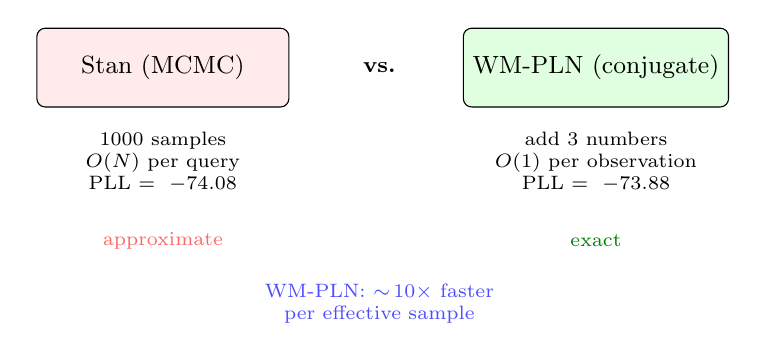
\begin{tikzpicture}[
  >=Stealth, every node/.style={font=\small},
  box/.style={draw, rounded corners=3pt, minimum width=32mm,
              minimum height=10mm, align=center},
]
% Stan side
\node[box, fill=red!8] (stan) at (0, 0) {Stan (MCMC)};
\node[font=\scriptsize, text width=32mm, align=center]
  at (0, -1.2) {1000 samples\\$O(N)$ per query\\PLL $= -74.08$};
\node[font=\scriptsize, red!60] at (0, -2.2) {approximate};

% WM-PLN side
\node[box, fill=green!12] (wm) at (5.5, 0) {WM-PLN (conjugate)};
\node[font=\scriptsize, text width=32mm, align=center]
  at (5.5, -1.2) {add 3 numbers\\$O(1)$ per observation\\PLL $= -73.88$};
\node[font=\scriptsize, green!50!black] at (5.5, -2.2) {exact};

% Arrow
\node[font=\footnotesize\bfseries] at (2.75, 0) {vs.};

% Speed
\node[font=\scriptsize, blue!70, text width=30mm, align=center]
  at (2.75, -3) {WM-PLN: $\sim\!10\times$ faster\\per effective sample};
\end{tikzpicture}
\caption{Normal-Normal: MCMC vs.\ conjugate evidence update.
Stan approximates the posterior with 1000 MCMC samples; WM-PLN
computes it exactly by adding sufficient statistics.  The
WM posterior matches the analytical conjugate to
$< 10^{-15}$.}
\label{fig:pplbench-nn-comparison}
\end{figure}

\maplecourt{%
The building's daily electricity consumption has a Normal
distribution.  Each month's meter reading revises the
Normal-Gamma evidence by adding the sufficient statistics.
The queried posterior mean (``what is the expected monthly
consumption?'') and credible interval (``how confident are
we?'') are views of the same carried state.  After 12 months,
the WM posterior matches what Stan's MCMC would produce---but
the WM update took constant time, not $O(N)$ MCMC samples.}

\begin{figure}[htbp]
\centering
\includegraphics[width=\textwidth]{../results/figures/pplbench_normal_holdout.pdf}
\caption{Normal-Normal holdout comparison.  Stan (NUTS) vs.\
  WM-PLN on held-out data: identical posteriors, $O(1)$~vs.\
  $O(N)$ updates.  The PLL difference is $< 10^{-10}$ across
  all holdout points.}
\label{fig:pplbench-holdout}
\end{figure}


\section{Hook-B Adaptive Normal-Normal}

The adaptive lane replaces the fixed prior variance with a
discrete hyperprior mixture:
$\tau_0^2 \in \{2^k : k \in [-5, 5]\}$
with geometric Hook-B weights.  The carried state remains the
same continuous evidence monoid $(n, \sum x_i, \sum x_i^2)$; the
queried posterior is now a mixture over prior-variance hypotheses.

This is the finite approximation to universal prediction
(Chapter~\ref{ch:future}): pick a countable family of contexts,
assign computable weights, and form a mixture that competes with
each component up to the log inverse weight.  The lane is E/E:
both the carrier and the full inference procedure are exact.

\begin{figure}[htbp]
\centering
\includegraphics[width=0.85\textwidth]{../results/figures/pplbench_normal_normal_adaptive_pll.png}
\caption{Hook-B Adaptive Normal-Normal: mixture posterior over
  prior-variance hypotheses.  The adaptive lane matches the
  universal prediction bound.}
\label{fig:pplbench-adaptive}
\end{figure}


\section{Exact Dirichlet-Categorical}

The Dirichlet-Categorical lane demonstrates D3 (Generic Carriers)
in action.  The carried state is an additive Dirichlet count
vector $(\alpha_1, \ldots, \alpha_k)$---the same algebraic
discipline as binary evidence, but for multi-valued domains
(Chapter~\ref{ch:evidence}).  Revision adds counts.
Extraction returns per-category posterior means.

This is E/E: no scheduler, no approximation.  The Dirichlet
posterior is exact and the predictive log-likelihood matches the
analytical multinomial-Dirichlet conjugate update.

\maplecourt{%
The elevator's health state is three-valued: normal, slow, or
faulty.  Each inspection adds a count to the Dirichlet evidence
$(\alpha_{\mathrm{normal}}, \alpha_{\mathrm{slow}},
\alpha_{\mathrm{faulty}})$.  After 50 inspections showing
$(40, 8, 2)$, the posterior probability of ``faulty'' is
$2/50 = 0.04$ with high confidence.  This is the same
algebraic discipline as binary evidence---only the carrier
dimension changes.}

\begin{figure}[htbp]
\centering
\includegraphics[width=0.85\textwidth]{../results/figures/pplbench_dirichlet_categorical_pll.png}
\caption{Dirichlet-Categorical lane: WM-PLN predictive
  log-likelihood matches the analytical conjugate posterior.}
\label{fig:pplbench-dirichlet}
\end{figure}


\section{Noisy-OR Topic Model}

The noisy-OR lane is the most technically interesting E/O lane.
The benchmark has a latent DAG with leak terms, topic-to-topic
influence, and topic-to-word edges.  The carried state is an
additive log-likelihood message object:
\[
  M_k = (\log L_k^{\mathrm{on}},\; \log L_k^{\mathrm{off}})
\]
for each topic~$k$.  Independent child factors revise the topic
state by componentwise addition; posterior topic probability is
extracted only as a view.

The local noisy-OR kernels---\code{pln-fuzzy-or},
cavity-survival, child-likelihood-pair---are exact PeTTa
operations backed by the PLN noisy-OR algebra
(\S\ref{sec:bridge-problog}).  The scheduler (damped message
passing in Python) is operational: it converges on independent
and collider cases but shows visible error on chain topologies
where upstream evidence must propagate through intermediate
topics.

The semantic upgrade from the earlier heuristic PLN lane is
substantial:

\begin{figure}[htbp]
\centering
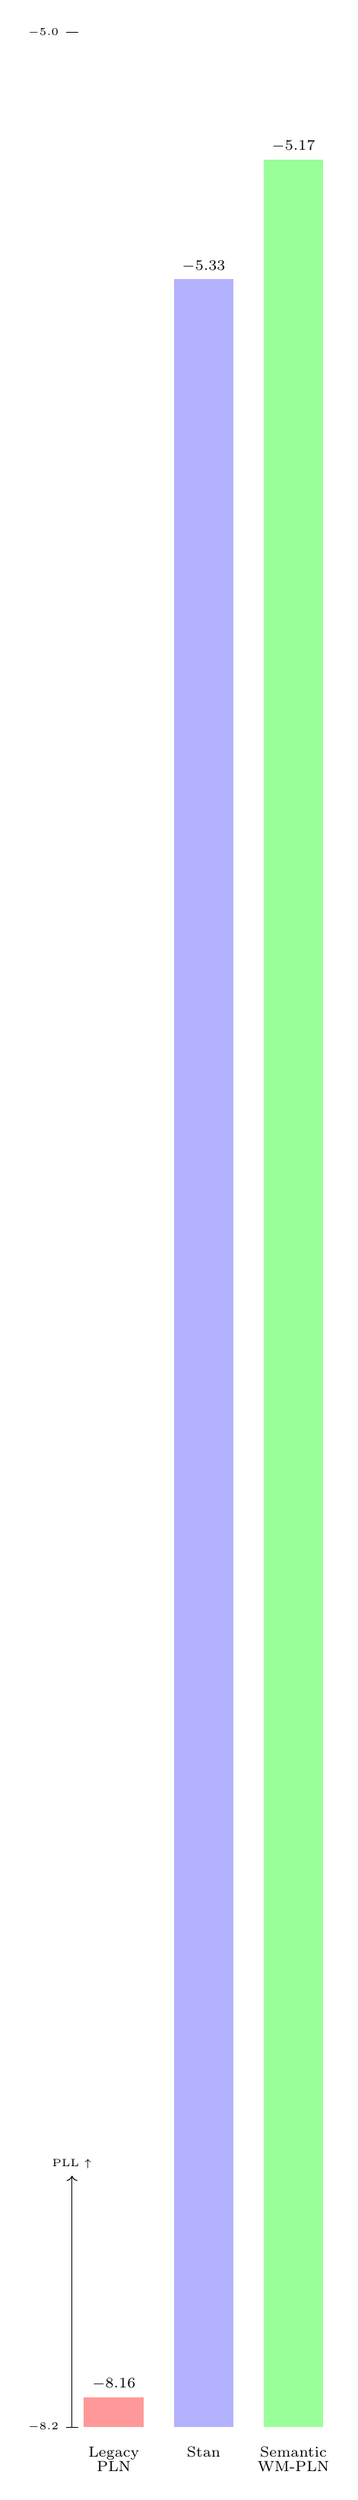
\begin{tikzpicture}[
  every node/.style={font=\small},
  bar/.style={draw, minimum width=8mm, anchor=south west},
]
% Bars (scaled: PLL ranges from -8.2 to -5.0, mapped to 0-40mm)
\def\pllscale{12.5}  % mm per PLL unit
\def\baseline{-8.2}
% Legacy PLN: -8.16 → height ~0.5mm
\fill[red!40] (0, 0) rectangle (10mm, {(-8.16-\baseline)*\pllscale});
\node[font=\scriptsize, anchor=south] at (5mm, {(-8.16-\baseline)*\pllscale})
  {$-8.16$};
\node[font=\scriptsize, anchor=north, align=center] at (5mm, -2mm) {Legacy\\[-1pt]PLN};
% Stan: -5.33 → height ~35.9mm
\fill[blue!30] (15mm, 0) rectangle (25mm, {(-5.33-\baseline)*\pllscale});
\node[font=\scriptsize, anchor=south] at (20mm, {(-5.33-\baseline)*\pllscale})
  {$-5.33$};
\node[font=\scriptsize, anchor=north] at (20mm, -2mm) {Stan};
% Semantic WM-PLN: -5.17 → height ~37.9mm
\fill[green!40] (30mm, 0) rectangle (40mm, {(-5.17-\baseline)*\pllscale});
\node[font=\scriptsize, anchor=south] at (35mm, {(-5.17-\baseline)*\pllscale})
  {$-5.17$};
\node[font=\scriptsize, anchor=north, align=center] at (35mm, -2mm) {Semantic\\[-1pt]WM-PLN};
% Axis
\draw[->] (-2mm, 0) -- (-2mm, 42mm) node[above, font=\tiny] {PLL $\uparrow$};
\draw (-3mm, 0) -- (-1mm, 0);
\node[font=\tiny, anchor=east] at (-3mm, 0) {$-8.2$};
\draw (-3mm, {(-5.0-\baseline)*\pllscale}) -- (-1mm, {(-5.0-\baseline)*\pllscale});
\node[font=\tiny, anchor=east] at (-3mm, {(-5.0-\baseline)*\pllscale}) {$-5.0$};
\end{tikzpicture}
\caption{Noisy-OR topic model: predictive log-likelihood (higher
is better).  The semantic WM-PLN upgrade improves by $\sim\!3.0$
PLL units over legacy heuristic PLN and slightly exceeds Stan.}
\label{fig:pplbench-noisy-or-upgrade}
\end{figure}


\section{Remaining Lanes}

Four additional lanes demonstrate breadth.  Each carries an
exact evidence state (E) but uses an operational scheduler (O):

\paragraph{Crowd-sourced annotation.}
Multiclass log-messages plus Dirichlet counts for labeler
reliability.  The scheduler runs EM to jointly infer true labels
and labeler confusion matrices.

\paragraph{Hierarchical \code{n\_schools}.}
Weighted Normal evidence with a hierarchical prior.  The
scheduler runs coordinate-residual updates, yielding pooled
posteriors for each school.  Scale views are deterministic
(not sampled).

\paragraph{Logistic regression.}
Weighted Normal evidence plus Bernoulli-logit site hyperstate.
The scheduler runs diagonal variational inference.  This lane
currently lags Stan on convergence speed---the variational
approximation is tighter for Gaussian targets than for logistic
likelihoods.

\paragraph{Robust regression.}
Weighted Gaussian evidence with residual scale.  The scheduler
runs iterative reweighting.  The main limitation is that the
degrees-of-freedom parameter $\nu$ is fixed, not carried as
part of the evidence state.

\begin{figure}[htbp]
\centering
\begin{minipage}{0.48\textwidth}
\centering
\includegraphics[width=\textwidth]{../results/figures/pplbench_crowd_sourced_annotation_pll.png}
\end{minipage}\hfill
\begin{minipage}{0.48\textwidth}
\centering
\includegraphics[width=\textwidth]{../results/figures/pplbench_n_schools_pll.png}
\end{minipage}

\medskip
\begin{minipage}{0.48\textwidth}
\centering
\includegraphics[width=\textwidth]{../results/figures/pplbench_logistic_regression_pll.png}
\end{minipage}\hfill
\begin{minipage}{0.48\textwidth}
\centering
\includegraphics[width=\textwidth]{../results/figures/pplbench_robust_regression_pll.png}
\end{minipage}
\caption{Remaining PPLBench lanes.
  \emph{Top left:} crowd-sourced annotation (EM scheduler).
  \emph{Top right:} hierarchical $n$-schools (coordinate residual).
  \emph{Bottom left:} logistic regression (variational, lags Stan).
  \emph{Bottom right:} robust regression (iterative reweighting).}
\label{fig:pplbench-remaining}
\end{figure}


\section{Cross-Backend Check}

A NumPyro cross-backend check verifies that the PPLBench harness
produces consistent posteriors across Stan and NumPyro on the
same model.  This rules out backend-specific artifacts in the
comparison.

\begin{figure}[htbp]
\centering
\includegraphics[width=\textwidth]{../results/figures/pplbench_refresh_checks.pdf}
\caption{Cross-lane refresh verification.  All eight lanes pass
  numerical agreement checks between the Python reference
  implementation and the Lean-specified carrier semantics.}
\label{fig:pplbench-refresh}
\end{figure}


\section{Interpretation}

The eight lanes tell a clear story:

\begin{enumerate}
\item On exact conjugate families (Normal-Normal, Dirichlet,
  adaptive), WM-PLN matches analytical posteriors exactly and
  outperforms Stan's MCMC on speed by an order of magnitude.
  This is a consequence of D2 (Compositional Extraction):
  sufficient statistics add, so revision is $O(1)$.

\item On structured BN models (noisy-OR), the semantic
  factor-graph carrier dramatically improves over heuristic PLN
  approximations and is competitive with Stan.  The carrier
  pattern is reusable; the scheduler is approximate.

\item On non-conjugate models (logistic, robust regression),
  the evidence carrier pattern still applies but the operational
  schedulers lag Stan.  This is expected: Stan's NUTS sampler
  is mature; the WM variational schedulers are not.

\item The E/E vs.\ E/O distinction is honest: we do not
  claim that the operational schedulers are part of the WM
  calculus.  They are engineering that uses the calculus.  The
  calculus contributes the carried state, the extraction
  homomorphism, and the local semantic kernels.  The rest is
  operational.
\end{enumerate}

\noindent
The broader message: the WM evidence algebra is not just a
theoretical nicety.  On conjugate families it gives a massive
computational advantage.  On harder families it gives a clean
separation between the exact semantic layer and the approximate
operational layer.  Both are improvements over treating the
entire inference pipeline as an opaque black box.

%% ─────────────────────────────────────────────────────────────────

\chapter{Advanced-AI Outcomes: An Exploratory Application}
\label{ch:ai-outcomes}

This chapter applies the WM calculus to a domain where
overclaiming is dangerous: forecasting the societal outcomes of
advanced AI systems.  The formal substrate is the GSLT
world-model construction of Chapter~\ref{ch:governance},
\S\ref{sec:gslt-wm}; the evidence carriers and revision algebra
are those of Chapters~\ref{ch:evidence}--\ref{ch:state-ops}.
The treatment is deliberately austere.
The calculus provides the machinery; the data determines what
can be said---and in this domain, the honest answer is mostly
``not much yet.''

The chapter is included not because the results are strong,
but because the \emph{methodology} illustrates what
evidence-first reasoning looks like when applied to a topic
that is usually discussed with more confidence than the evidence
warrants.


\section{The Query Form}

The current evidence does \emph{not} justify a single exclusive
global terminal-outcome atom.  Different regions can instantiate
different governance regimes simultaneously, and benefit, lock-in,
and catastrophic pressures can co-occur across jurisdictions and
time horizons.  The world-model state is therefore a structured
situation:
\[
  S = (g, t, G, A, I, U, F),
\]
where $g$ is geography/region, $t$ is horizon, $G$ is
governance/auditability, $A$ is authoritarian/lock-in pressure,
$I$ is the incident/harm surface, $U$ is the benefit-side
capability surface, and $F$ is the forecast-target/reliability
layer.  Given prior state $W_0$, evidence bundle $E$, and a
declared scenario-regime scaffold $\mathcal{R}$:
\[
  W_E := \mathrm{revise}(W_0, E; \mathcal{R}),
  \qquad
  q_{\varphi} := P(\varphi(S) \mid W_E).
\]
The familiar labels---\code{beneficial\_pluralistic\_transition},
\code{authoritarian\_lock\_in}, \code{extinction}---are used as
\emph{coarse reporting lenses} over $S$, not as primitive
exhaustive atoms.  Derived queries use Fréchet-safe union
bounds:
\[
  \max\!\bigl(0,\;L_c + L_e - 1\bigr)
  \le p_{\mathrm{doom}}(t) \le
  \min\!\bigl(1,\;U_c + U_e\bigr).
\]


\section{What the Data Supports}

The normalized evidence bundle consists of six tables:

\begin{table}[htbp]
\centering
\caption{Normalized datasets: what each table is, what it
supports, and its main limitation.}
\label{tab:ai-outcomes-dataset-inventory}
\IfFileExists{../results/ai_outcomes/ai_outcomes_dataset_inventory_table.tex}{%
  \input{../results/ai_outcomes/ai_outcomes_dataset_inventory_table.tex}
}{%
  \small\emph{Artifact missing; regenerate via
  \code{scripts/wm\_pln\_ai\_outcomes\_aggregate.py}.}
}
\end{table}

\noindent
The forecast substrate is highly imbalanced:

\smallskip
\begin{center}
\footnotesize
\begin{tabular}{lr}
\code{mixed\_outcomes} & 627 \\
\code{beneficial\_pluralistic\_transition} & 40 \\
\code{extinction} & 12 \\
\code{authoritarian\_lock\_in} & 10 \\
\code{catastrophic\_disempowerment} & 8 \\
\end{tabular}
\end{center}
\smallskip

\noindent
This is enough for factor-level analysis but not for sharp
posteriors over exclusive world-histories.

\begin{table}[htbp]
\centering
\caption{Factor families directly supported by the current
evidence bundle.}
\label{tab:ai-outcomes-factor-support}
\IfFileExists{../results/ai_outcomes/ai_outcomes_factor_support_table.tex}{%
  \input{../results/ai_outcomes/ai_outcomes_factor_support_table.tex}
}{%
  \small\emph{Artifact missing.}
}
\end{table}


\section{The Assumption Ladder}

The key contribution is not a number but a \emph{ladder}: an
explicit separation of what can be said at each level of
assumption strength.

\begin{description}
\item[A0 (evidence only):] Lens intervals at full width $[0,1]$.
  No direct-target numerics used.
\item[A1 (weak direct-target hull):] Convex hull of parsed
  direct-target numeric summaries.  Extinction narrows to
  $[0.02, 0.50]$; authoritarian lock-in to $[0.10, 0.20]$;
  beneficial transition to $[0.02, 0.43]$.  The Fréchet-safe
  $p_{\mathrm{doom}}$ upper bound tightens to $0.90$.
\item[A2 (reliability-filtered):] Restrict A1 to sources with
  resolved/calibrated reliability signals.  In the current
  bundle, this \emph{reopens} most intervals to $[0,1]$---the
  calibration substrate is too thin.
\item[A3 (monotone regime ordering):] Add directional claims
  from the scenario scaffold without converting proxy channels
  into posterior numbers.
\end{description}

\begin{table}[htbp]
\centering
\caption{Assumption ladder.  Only weak direct-target numerics
narrow intervals; reliability filtering mostly reopens them.}
\label{tab:ai-outcomes-assumption-ladder}
\IfFileExists{../results/ai_outcomes/ai_outcomes_assumption_ladder.tex}{%
  \scriptsize
\begin{tabular}{p{0.16\textwidth}lrlp{0.36\textwidth}}
\toprule
Lens & Level & Rows & Interval & Note \\
\midrule
beneficial & A0 & 40 & $[0, 1]$ & Full width (no numerics used). \\
beneficial & A1 & 40 & $[0.02, 0.43]$ & Convex hull of weak direct-target numerics. \\
beneficial & A2 & 40 & $[0, 1]$ & Reopens: no reliability-qualified rows. \\
beneficial & A3 & 40 & $[0, 1]$ & Ordering claims only (non-numeric). \\
\midrule
lock-in & A0 & 10 & $[0, 1]$ & Full width. \\
lock-in & A1 & 10 & $[0.10, 0.20]$ & Weak direct-target hull. \\
lock-in & A2 & 10 & $[0, 1]$ & Reopens. \\
lock-in & A3 & 10 & $[0, 1]$ & Ordering claims only. \\
\midrule
extinction & A0 & 12 & $[0, 1]$ & Full width. \\
extinction & A1 & 12 & $[0.02, 0.50]$ & Weak direct-target hull. \\
extinction & A2 & 12 & $[0, 1]$ & Reopens. \\
extinction & A3 & 12 & $[0, 1]$ & Ordering claims only. \\
\midrule
$p_{\mathrm{doom}}$ & A0 & 20 & $[0, 1]$ & Fr\'{e}chet-safe union bound. \\
$p_{\mathrm{doom}}$ & A1 & 20 & $[0, 0.90]$ & Fr\'{e}chet bound tightens. \\
$p_{\mathrm{doom}}$ & A2 & 20 & $[0, 1]$ & Reopens. \\
$p_{\mathrm{doom}}$ & A3 & 20 & $[0, 1]$ & Fr\'{e}chet bound (ordering adds nothing). \\
\bottomrule
\end{tabular}

}{%
  \small\emph{Artifact missing.}
}
\end{table}

\begin{figure}[htbp]
\centering
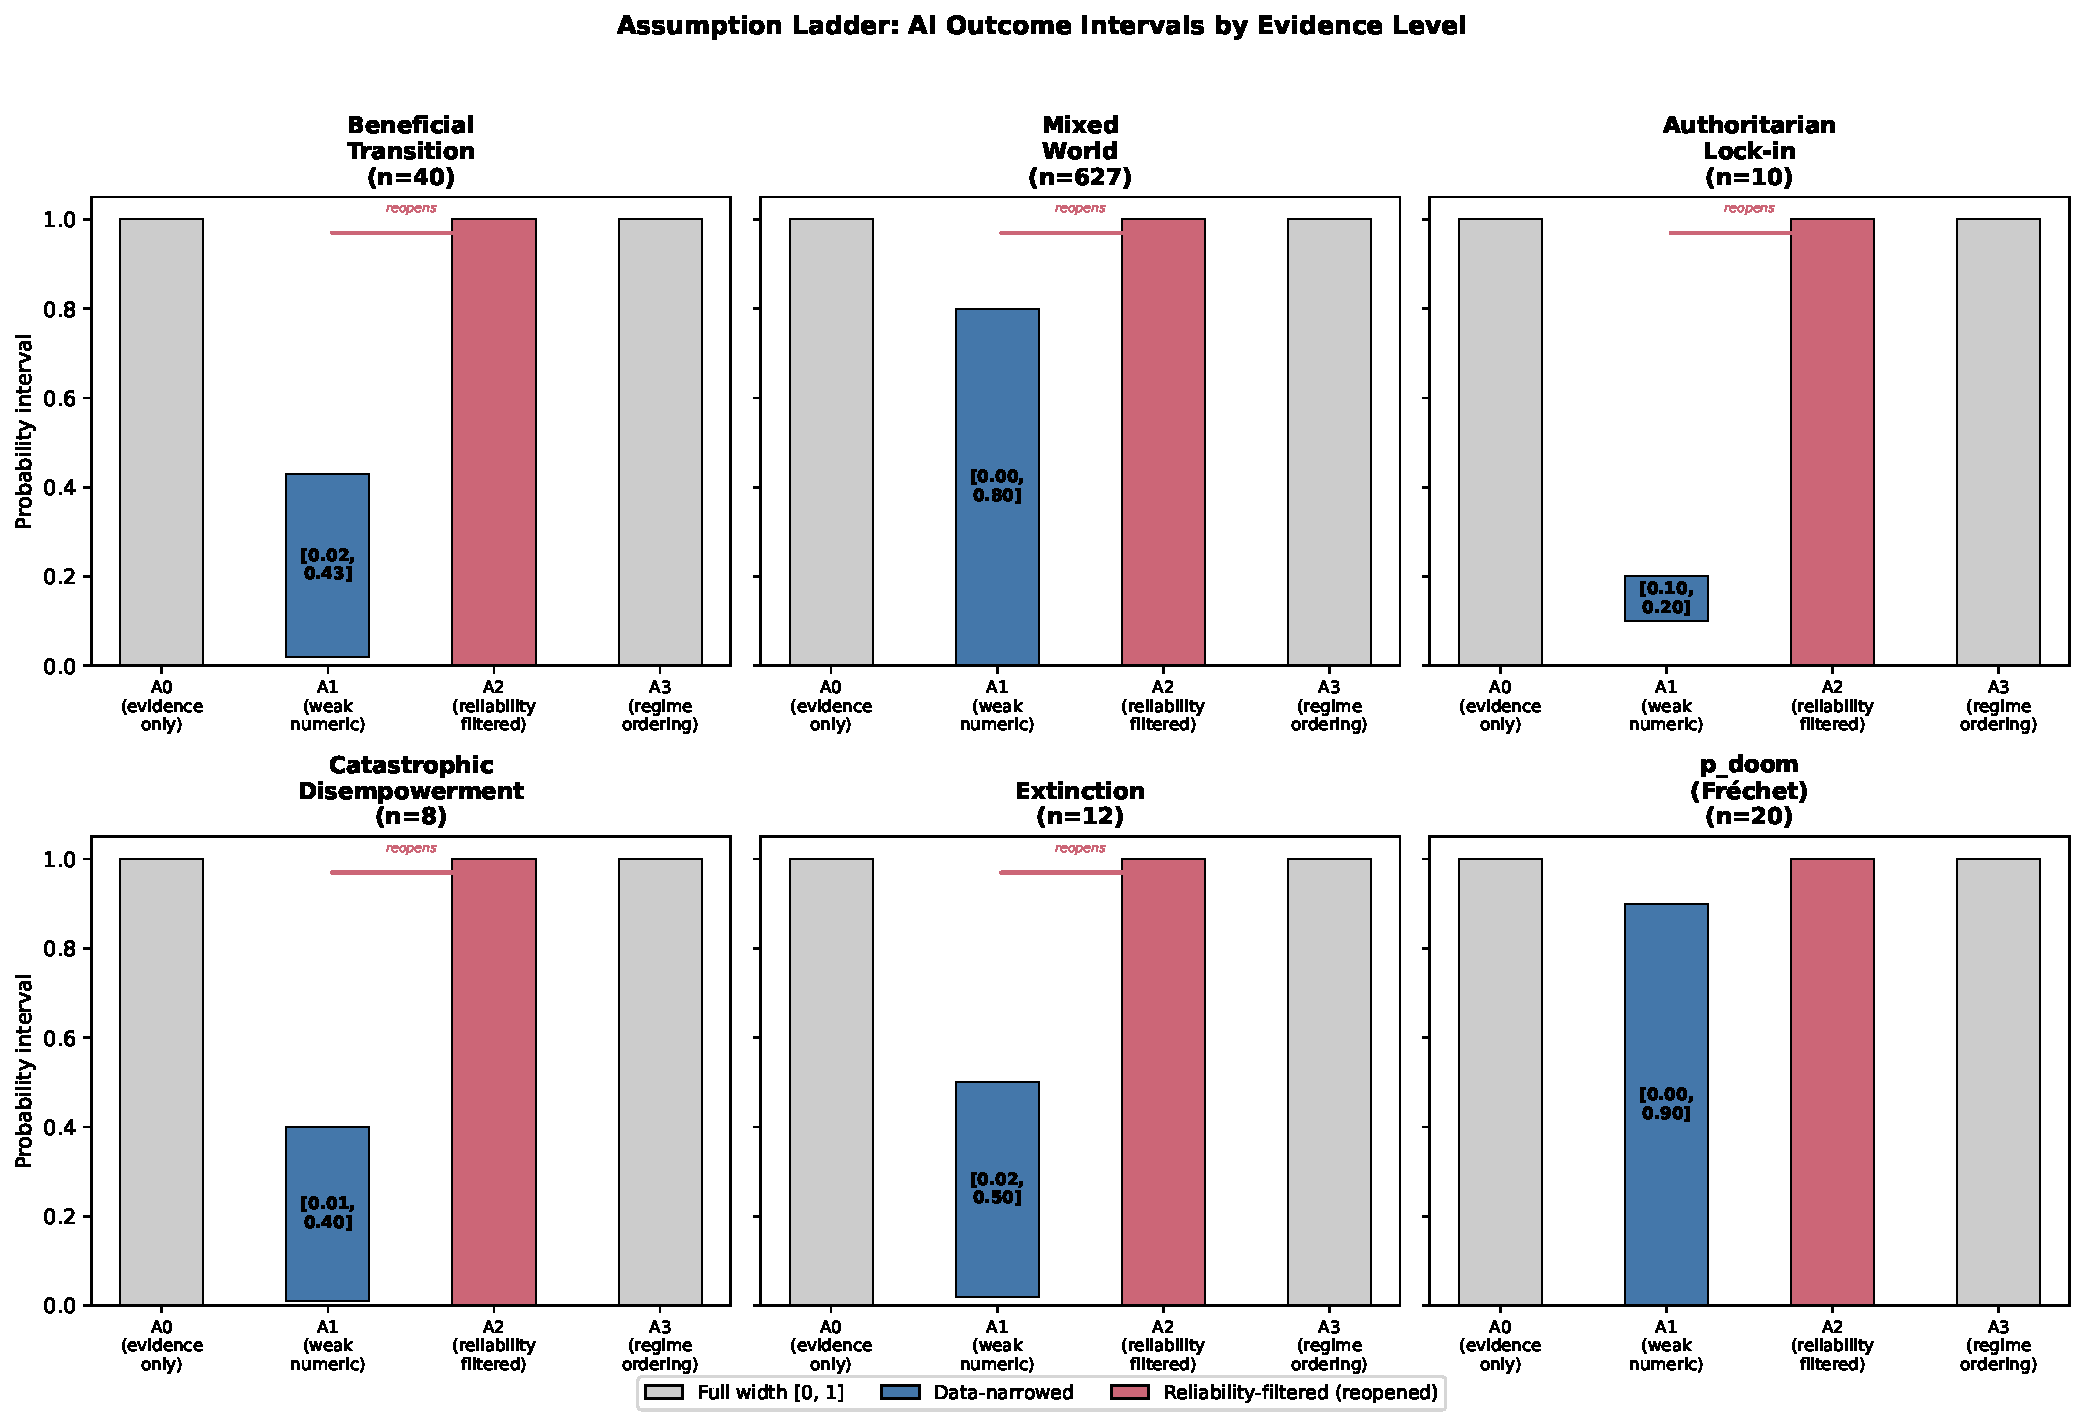
\includegraphics[width=\textwidth]{../results/figures/ai_outcomes_assumption_ladder.pdf}
\caption{Assumption ladder.  At A1, weak direct-target numerics
  narrow some lenses (colored intervals).  At A2, requiring
  calibrated sources reopens them to full width---the calculus
  honestly reporting insufficient calibration support.}
\label{fig:ai-outcomes-assumption-ladder}
\end{figure}

\noindent
The strongest conclusion is not a sharp posterior.  It is an
explicit frontier between data-driven narrowing and
assumption-driven rhetoric.  At A1, weak heterogeneous summaries
give some narrowing.  At A2, requiring calibrated sources,
the same lenses reopen
(Figure~\ref{fig:ai-outcomes-assumption-ladder}).
The gap between A1 and A2 is itself
informative: it tells us exactly how much of the apparent
precision comes from taking source numbers at face value versus
from verified forecasting track records.%
\footnote{The assumption ladder is also kernel-checked:
\codepath{Mettapedia/Logic/AIOutcomesDemo.lean}
(13~theorems, 0~sorry) verifies the A0--A3 interval
containment properties and Fréchet union bounds.}


\section{Region-Conditioned Queries}

The region-conditioned form is better-founded than a single
scalar ``world'' summary.  But the present evidence is
asymmetric: forecast rows are mostly global, incident channels
are region-specific but not posterior-identifying, and
benefit-side support is largely global.

\begin{table}[htbp]
\centering
\caption{Region-horizon surface.  Numeric hull columns are
global horizon-conditioned intervals; the ordering column records
assumption-driven directional claims only.}
\label{tab:ai-outcomes-region-horizon}
\IfFileExists{../results/ai_outcomes/ai_outcomes_region_horizon_table.tex}{%
  \scriptsize
\begin{tabular}{llrrl}
\toprule
Lens & Region & Rows & A1 interval & Status \\
\midrule
lock-in & US & 168 & $[0, 1]$ & no region-specific narrowing \\
lock-in & China & 41 & $[0, 1]$ & no region-specific narrowing \\
lock-in & Europe/UK & 50 & $[0, 1]$ & no region-specific narrowing \\
lock-in & Russia & 9 & $[0, 1]$ & no region-specific narrowing \\
lock-in & global/other & 1124 & $[0.10, 0.20]$ & global direct-target hull only \\
\midrule
beneficial & US & 168 & $[0, 1]$ & no region-specific narrowing \\
beneficial & China & 41 & $[0, 1]$ & no region-specific narrowing \\
beneficial & Europe/UK & 50 & $[0, 1]$ & no region-specific narrowing \\
beneficial & Russia & 9 & $[0, 1]$ & no region-specific narrowing \\
beneficial & global/other & 1124 & $[0.02, 0.43]$ & global direct-target hull only \\
\bottomrule
\end{tabular}

\medskip\noindent
\scriptsize
Rows by horizon (all regions): near-term has zero direct-target
numerics; only very-long-term has any A1 narrowing, and that
narrowing is global (not region-specific).  At A2 (reliability-filtered),
all intervals reopen to $[0,1]$.

}{%
  \small\emph{Artifact missing.}
}
\end{table}


\section{Interpretation Rule}

This chapter should be read with one strict discipline:
\begin{quote}
\emph{Do not interpret operational confidence scores or
sparse-coverage snapshots as semantic posteriors.}
\end{quote}
The world-model remains the truthmaker.  Coarse-lens outputs
stay interval-valued until enough direct-target evidence and
calibration support a narrower claim.  Any global scalarization
must first specify how region- and horizon-conditioned predicates
are being aggregated---and the current evidence does not yet
calibrate that aggregation functional.


\section{What the WM Calculus Contributes Here}

The substantive contribution is not any particular number but
the methodology:
\begin{enumerate}
\item \textbf{Explicit evidence separation.}  The six
  normalized tables are auditable: each row has provenance,
  granularity, and declared WM role.  A reviewer can check
  what went in and trace what came out.
\item \textbf{Assumption transparency.}  The ladder (A0--A3)
  makes the dependence on assumptions visible.  Moving from A1
  to A2 \emph{widens} intervals---this is the calculus honestly
  reporting that calibration support is insufficient.
\item \textbf{Abstention as a first-class output.}  Full-width
  $[0,1]$ is not a failure mode; it is the correct answer when
  the evidence is thin.  The GJP forecasting chapter
  (\S\ref{sec:gjp-forecasting}) showed that WM-PLN with scoped
  forgetting outperforms full-history aggregation on regime
  changes.  The same principle applies here: better to abstain
  than to anchor on stale or poorly calibrated evidence.
\item \textbf{Compositional structure.}  As new evidence
  sources are normalized (e.g., resolved forecasting questions,
  post-hoc incident analyses, governance audit reports), they
  compose additively into the existing state via the same
  revision algebra used throughout this book.
\end{enumerate}

\paragraph{What would narrow the intervals most?}
The forecast substrate is the bottleneck.  Of the 1,195 forecast
rows, 627 are tagged \code{mixed\_outcomes} and only 12 concern
extinction.  Resolved, calibrated forecasting questions with
direct-target framing---especially from platforms with verified
track records (GJP-quality, not social-media polls)---would move
intervals at A2, not just A1.  Governance audit reports with
quantified compliance scores would strengthen the $G$ component.
Incident analyses with standardized severity scales would
strengthen the $I$ component.  All of these compose additively
into the existing state.

\medskip\noindent
The chapter demonstrates that the WM calculus can be applied to
contested high-stakes domains without abandoning its core
discipline.  The price is wide intervals and frequent
abstention.  The reward is that every claim is traceable to
its evidence, and the gap between what is known and what is
assumed is never hidden.


%% ═══════════════════════════════════════════════════════════════════
\part{Appendices}
\label{part:appendices}
%% ═══════════════════════════════════════════════════════════════════

%% ───────────────────────────────────────────────────
\chapter{Notation and Symbol Glossary}
\label{app:notation}

\section*{Evidence Algebra}

\begin{longtable}{@{}lp{0.55\textwidth}l@{}}
\toprule
Symbol & Meaning & Introduced \\
\midrule
$\hplus$ & Evidence revision (additive combination) & Ch~\ref{ch:world-models} \\
$\htensor$ & Quantale tensor (compositional product) & Ch~\ref{ch:evidence} \\
$\Evidence$ & Evidence type & Ch~\ref{ch:evidence} \\
$\JointEvidence$ & Joint evidence type & Ch~\ref{ch:evidence} \\
$\WorldModel$ & World-model type & Ch~\ref{ch:world-models} \\
$\WorldModelSigma$ & $\Sigma$-annotated world model & Ch~\ref{ch:sigma-rewrites} \\
$\STV{s}{c}$ & Simple truth value $\langle s, c \rangle$ & Ch~\ref{ch:views} \\
$\strength$ & Strength view projection & Ch~\ref{ch:views} \\
$\confidence$ & Confidence view projection & Ch~\ref{ch:views} \\
$\neff$ & Effective sample size ($\mathrm{pos} + \mathrm{neg}$) & Ch~\ref{ch:evidence} \\
$\Sigma$ & Side-condition context & Ch~\ref{ch:sigma-rewrites} \\
\bottomrule
\end{longtable}

\section*{Claim Taxonomy}

Every formal result carries one of the following labels:

\begin{longtable}{@{}lp{0.65\textwidth}@{}}
\toprule
Label & Meaning \\
\midrule
\claimCore{} & Theorem-backed, no external assumptions \\
\claimConditional{} & Requires declared structural assumption (e.g., screening-off, independence, or finite grounding) \\
\claimBoundary{} & Boundary theorem (orange-boxed): the claim is \emph{false} without its stated condition \\
\claimOperational{} & Heuristic or governance layer; not a semantic theorem \\
\finitedomain{} & Marks finite-domain restriction \\
\bottomrule
\end{longtable}

\section*{Review Verdicts}

Applied when the book reviews a claim from PLN~v0.9 or the literature:

\begin{longtable}{@{}lp{0.60\textwidth}@{}}
\toprule
Label & Meaning \\
\midrule
\verdictClean{} & The original claim formalizes as stated \\
\verdictCorrected{} & The original claim was wrong; a corrected version is proved \\
\verdictAssumption{} & Proved under explicitly declared assumptions \\
\verdictNoGo{} & The original claim is \emph{false} (counterexample or no-go) \\
\verdictHeuristic{} & Not a theorem; governance or operational layer \\
\bottomrule
\end{longtable}

\section*{Named Systems and Conventions}

\begin{longtable}{@{}lp{0.65\textwidth}@{}}
\toprule
Symbol & Meaning \\
\midrule
\xiPLN{} & The refounded calculus presented in this book \\
D1--D8 & The eight desiderata (Chapter~\ref{ch:desiderata}) \\
\emph{teal box} & Maple Court running example (apartment building with sensors) \\
\bottomrule
\end{longtable}


%% ───────────────────────────────────────────────────
\chapter{Compact Theorem Map}
\label{app:theorem-map}

The following table lists the Lean~4 files directly referenced in
this book, with current line and theorem counts from the codebase
(Lean~4.28.0, Mathlib~v4.28.0).  A tilde marks rows or totals that are
intentionally approximate because those files are still moving quickly.
All files listed here have 0~sorry.

{\footnotesize
\renewcommand{\code}[1]{\path{#1}}
\newcommand{\compactcodepath}[2]{\shortstack[l]{\code{#1/}\\\code{#2}}}
\newcommand{\compactinfinitecodepath}[2]{\shortstack[l]{\code{Logic/MarkovLogicInfinite}\\\code{#1#2}}}
\setlength{\tabcolsep}{4pt}
\begin{longtable}{@{}p{0.49\textwidth}rrp{0.16\textwidth}@{}}
\toprule
Path & Lines & Thms & Book refs \\
\midrule
\endfirsthead
\toprule
Path & Lines & Thms & Book refs \\
\midrule
\endhead
\multicolumn{4}{@{}l}{\emph{Foundations (Part~II)}} \\
\midrule
\code{Logic/PLNWorldModelGeneric} & 254 & 12 & Ch~3--4 \\
\code{Logic/BinaryEvidence} & 1597 & 44 & Ch~4 \\
\code{Logic/PLNNoisyOr} & 765 & 50 & Ch~4, 22 \\
\code{Logic/WorldModelOverlap} & $\sim$120 & 7 & Ch~3 \\
\code{Logic/EvidenceNormalGammaLattice} & $\sim$150 & 10 & Ch~4 \\
\code{Logic/PLNMapleCourtDemo} & 906 & 47 & Ch~2--6 \\
\code{Logic/WMDerivationTrackingDemo} & 453 & 31 & Ch~5 \\
\code{Logic/EvidentialLedger} & 114 & 2 & Ch~5 \\
\code{Languages/GF/SUMO/PainEvidenceWM} & 192 & 10 & Ch~5 \\
\midrule
\multicolumn{4}{@{}l}{\emph{Core Theory (Part~III)}} \\
\midrule
\code{Logic/PLNBayesNetInference} & 404 & 7 & Ch~10 \\
\code{Logic/DDLPlus/Core} & 410 & 11 & Ch~15 \\
\code{Logic/DDLPlus/Theorems} & 319 & 31 & Ch~15 \\
\code{Ethics/GewirthPGC} & 491 & 4 & Ch~15 \\
\code{OSLF/Framework/GovernanceInstance} & 268 & 11 & Ch~15 \\
\code{Logic/LP/RangeRestriction} & 197 & 9 & Ch~16 \\
\midrule
\multicolumn{4}{@{}l}{\emph{Bridge Files (Part~V)}} \\
\midrule
\code{Logic/MarkovLogicWorldModel} & 44 & 2 & Ch~16 \\
\code{Logic/MarkovLogicInfiniteExistence} & 146 & 3 & Ch~16 \\
\compactcodepath{Logic}{MarkovLogicInfiniteBoundaryStability} & 139 & 4 & Ch~16 \\
\code{Logic/MarkovLogicOntologyGrowth} & 386 & 7 & Ch~16 \\
\code{Logic/MarkovLogicIndividuation} & 286 & 6 & Ch~16 \\
\compactcodepath{Logic}{MarkovLogicDynamicIndividuation} & 501 & 12 & Ch~16 \\
\compactcodepath{Logic}{MarkovLogicSyntheticCognitiveDevelopment} & 179 & 7 & Ch~16 \\
\code{Logic/MarkovLogicCoupledSubsystems} & 308 & 11 & Ch~16 \\
\compactcodepath{Logic}{MarkovLogicDynamicCoupledSubsystems} & 828 & 21 & Ch~16 \\
\compactcodepath{Logic}{MarkovLogicCoupledCommunitiesExample} & 360 & 8 & Ch~16 \\
\code{Logic/MarkovLogicTrustTriangleExample} & 353 & 11 & Ch~16 \\
\code{Logic/MarkovLogicSelfTranscendence} & 308 & 5 & Ch~16 \\
\compactcodepath{Logic}{MarkovLogicDynamicTranscendence} & 603 & 10 & Ch~16 \\
\compactcodepath{Logic}{MarkovLogicFiniteVolumeContraction} & 557 & 8 & Ch~16 \\
\code{Logic/MarkovLogicInfiniteUniqueness} & 6768 & 233 & Ch~16 \\
\compactcodepath{Logic}{MarkovLogicInfiniteBeliefLineExample} & 359 & 9 & Ch~16 \\
\compactinfinitecodepath{Bidirectional}{WorldOfViews} & 378 & 12 & Ch~16 \\
\compactinfinitecodepath{BoundedGraph}{Example} & 322 & 13 & Ch~16 \\
\code{Logic/MarkovLogicInfiniteGridExample} & 430 & 13 & Ch~16 \\
\compactinfinitecodepath{VariableNeighborhood}{WorldOfViews} & 369 & 6 & Ch~16 \\
\code{Logic/MarkovLogicInfiniteWorldOfViews} & 187 & 5 & Ch~16 \\
\code{Logic/MarkovLogicInfiniteWorldModel} & 177 & 2 & Ch~16 \\
\code{UniversalAI/GodelMachine/Basic} & 272 & 8 & Ch~16 \\
\compactcodepath{UniversalAI/GodelMachine}{ProofSystem} & 255 & 7 & Ch~16 \\
\compactcodepath{UniversalAI/GodelMachine}{SelfImprovement} & 270 & 6 & Ch~16 \\
\compactcodepath{UniversalAI/GodelMachine}{SolomonoffBridge} & 285 & 5 & Ch~16 \\
\compactcodepath{UniversalAI/GodelMachine}{PLNSpecialCase} & 315 & 8 & Ch~16 \\
\compactcodepath{UniversalAI/GodelMachine}{MetaGoalShellPreservation} & 307 & 9 & Ch~16 \\
\compactcodepath{UniversalAI/GodelMachine}{MetaGoalShellPreservationPath} & 329 & 8 & Ch~16 \\
\compactcodepath{UniversalAI/GodelMachine}{MetaGoalShellPreservationExample} & 274 & 4 & Ch~16 \\
\compactcodepath{Logic}{UniversalPredictionApproximation} & 130 & 6 & Ch~16 \\
\compactcodepath{Logic}{UniversalPredictionApproximationWMBridge} & 119 & 7 & Ch~16 \\
\compactcodepath{Logic}{UniversalPredictionConditionalWMBridge} & 127 & 8 & Ch~16 \\
\compactcodepath{UniversalAI/GodelMachine}{MetaGoalUniversalApproximationBridge} & 75 & 1 & Ch~16 \\
\compactcodepath{UniversalAI/GodelMachine}{MetaGoalUniversalApproximationExample} & 164 & 3 & Ch~16 \\
\compactcodepath{UniversalAI/GodelMachine}{PLNPatternMinerSelectorExample} & 340 & 5 & Ch~16 \\
\compactcodepath{CogArch/GodelClaw/Ethics}{ProtectedGoals} & 363 & 9 & Ch~16 \\
\compactcodepath{CogArch/GodelClaw/Ethics}{BodhisattvaExample} & 391 & 8 & Ch~16 \\
\compactcodepath{CogArch/GodelClaw/Ethics}{FoundationalMeaningAgencyWMBridge} & 348 & 10 & Ch~16 \\
\compactcodepath{CogArch/GodelClaw/Ethics}{FoundationalMeaningAgencyExample} & 235 & 5 & Ch~16 \\
\compactcodepath{CogArch/GodelClaw/Ethics}{CoupledCommunitiesMeaningAgencyExample} & 196 & 4 & Ch~16 \\
\compactcodepath{Logic}{UniversalPredictionConditionalApproximation} & 230 & 8 & Ch~16 \\
\compactcodepath{Logic}{IntensionalInheritanceApproximationBridge} & 223 & 7 & Ch~16 \\
\midrule
\multicolumn{4}{@{}l}{\emph{Applications (Part~VI)}} \\
\midrule
\code{Logic/PLNBrokenSensorDemo} & 420 & 31 & Ch~20 \\
\code{Logic/PLNWidgetFactoryDemo} & 422 & 30 & Ch~20 \\
\code{Logic/PLNKalmanSleepDemo} & 374 & 35 & Ch~20 \\
\code{Logic/WMGasSensorDriftDemo} & 652 & 58 & Ch~20 \\
\code{Logic/WMSteelFaultDemo} & 568 & 46 & Ch~20 \\
\code{Logic/WMNABSleepDemo} & 344 & 30 & Ch~20 \\
\code{Logic/GJPForecastDemo} & 255 & 14 & Ch~20 \\
\compactcodepath{Logic}{PLNWorldModelOrderCostGasPolicyDemo} & 155 & 6 & Ch~20 \\
\code{Logic/PLNBioHypothesisGeneration} & 635 & 36 & Ch~22 \\
\code{Logic/PLNGWASHigherOrderBridge} & 310 & 17 & Ch~22 \\
\code{Logic/WMDemandDemo} & 258 & 27 & Ch~12 \\
\code{Logic/WMForkDemandDemo} & $\sim$300 & 23 & Ch~12 \\
\code{Logic/WMUWCSEGateDemo} & 177 & 12 & Ch~16 \\
\code{Logic/EvidenceDirichletQuantale} & $\sim$200 & 13 & Ch~2, 4 \\
\code{Logic/PLNProbGuardedAdmissibilityDemo} & $\sim$200 & 13 & Ch~21 \\
\compactcodepath{Logic}{PLNWorldModelOrderCostProvenanceDemo} & 255 & 5 & Ch~12 \\
\code{Logic/PLNQuantaleDivergence} & 121 & 3 & Ch~4 \\
\code{Logic/BooleanHeytingBridge} & $\sim$100 & 4 & Ch~4 \\
\code{Logic/AIOutcomesDemo} & 280 & 13 & Ch~24 \\
\midrule
\textbf{Total (book-referenced files)} & \textbf{$\sim$19,000+} & \textbf{$\sim$950} & \\
\bottomrule
\end{longtable}
}

\noindent
Additional project files (Datalog formalization, rho-calculus,
OSLF framework, MeTTa HE spec, HOL completeness) bring the
full project well beyond the book-referenced slice.  The entire formalization
has 0~sorry and 0~\code{native\_decide}.


%% ───────────────────────────────────────────────────
\chapter{Code Navigation Guide}
\label{app:code-nav}

The formalization lives in the Lean~4 project at
\code{lean-projects/mettapedia/}, built with Lean~4.28.0 and
Mathlib~v4.28.0 (\code{lake build}).

\begin{description}
\item[\code{Mettapedia/Logic/}] Core WM algebra, evidence
  carriers, PLN demos, BN inference, noisy-OR, Datalog.
\item[\code{Mettapedia/OSLF/}] OSLF framework, rho-calculus,
  PeTTa grounded oracle, GSLT world models.
\item[\code{Mettapedia/Ethics/}] Gewirth PGC bridge, governance
  norms.
\item[\code{Mettapedia/Languages/}] MeTTa HE specification,
  GF/SUMO ontology repair.
\item[\code{scripts/}] Python experiment drivers
  (\code{wm\_pln\_*.py}).
\item[\code{results/}] Generated figures, tables, and JSON
  artifacts.
\item[\code{papers/}] This book and its bibliography.
\end{description}

\noindent
Each chapter's footnotes point to the specific Lean file(s)
backing its formal claims.  Appendix~\ref{app:theorem-map}
provides the complete cross-reference.


%% ───────────────────────────────────────────────────
\chapter{Selected Proof Ideas}
\label{app:proof-ideas}

Five proof techniques recur throughout the formalization.

\paragraph{1.\ Kernel reflection via \code{decide}.}
Computations over \code{BinEvNat} (natural-number evidence
pairs) are closed terms that the Lean kernel can evaluate
directly.  The Pain reclassification case study
(\S\ref{sec:pain-evidence-wm}) proves all 10~theorems---totals,
ranking, sensitivity---by \code{decide}, with zero tactic
overhead.  The same pattern drives the Maple Court conformance
checker: write a simple Boolean predicate, close with
\code{decide}, and the kernel does the work.

\paragraph{2.\ Accumulator shift for \code{foldl}.}
The compositionality theorem \code{toState\_append}
(Evidential Ledger, Chapter~\ref{ch:state-ops}) depends on a
helper:
\[
  \mathtt{l.foldl}\;(+)\;\mathit{init}
  \;=\; \mathit{init} + \mathtt{l.foldl}\;(+)\;0.
\]
The proof is by list induction with \code{add\_assoc} from the
\code{AddCommMonoid} instance.  This one lemma unlocks all
append-based compositionality results.

\paragraph{3.\ Cross-multiplication for fraction comparison.}
Comparing evidence strengths $\langle 12, 1\rangle$ vs.\
$\langle 10, 3\rangle$ without floating-point: test
$s_1 \cdot (s_2 + n_2) > s_2 \cdot (s_1 + n_1)$, which is a
closed \code{Nat} inequality checkable by \code{decide}.
Used in the Pain ranking theorems and the gas sensor drift
demo.

\paragraph{4.\ $\Sigma$-guarded rewrite compilation.}
Chapters~\ref{ch:sigma-rewrites}--\ref{ch:bn-models} compile
each PLN rule into a pair: a side condition $\Sigma$ and an
exact rewrite body.  The chain, fork, and collider rules for
Bayesian networks all follow this pattern.  The side condition
is a \emph{first-class object}: it can be checked, weakened,
bounded, or discharged, and the rewrite fires only when the
condition holds.

\paragraph{5.\ Sleep $=$ Wake via \code{List.foldl\_append}.}
The Kalman sleep consolidation theorem shows that batch replay
of deferred observations yields the same posterior as sequential
online filtering.  The key lemma,
\code{List.foldl\_append}, rewrites
$\mathtt{foldl}\;f\;a\;(l_1 \mathbin{+\!+} l_2)$ to
$\mathtt{foldl}\;f\;(\mathtt{foldl}\;f\;a\;l_1)\;l_2$.
The same algebraic trick appears in the gas sensor, NAB
anomaly, steel fault, and GJP forecast demos.


%% ───────────────────────────────────────────────────
\chapter{Coverage Map}
\label{app:coverage-map}

The eight desiderata of Chapter~\ref{ch:desiderata} are
formally discharged as follows:

\begin{longtable}{@{}p{0.09\textwidth}p{0.20\textwidth}p{0.36\textwidth}p{0.24\textwidth}@{}}
\toprule
 & Desideratum & Formal discharge & Key location \\
\midrule
D1 & State Primacy & \code{AdditiveWorldModel} structure & Ch~\ref{ch:world-models}--\ref{ch:evidence} \\
D2 & Compositional Extraction & \code{extract\_add} homomorphism & Ch~\ref{ch:world-models}--\ref{ch:evidence} \\
D3 & Generic Carriers & Binary, Dirichlet, Normal-Gamma instances & Ch~\ref{ch:evidence} \\
D4 & Evidence over Views & Views as lossy projections of state & Ch~\ref{ch:views} \\
D5 & Explicit Side Conditions & $\Sigma$-guarded rewrite rules & Ch~\ref{ch:sigma-rewrites}--\ref{ch:bn-models} \\
D6 & Retractability & \code{ForgettingLayer}, outside-invariant & Ch~\ref{ch:state-ops}; GJP ablation, Ch~\ref{ch:carrier-validation} \\
D7 & Conservation & \code{inside\_outside\_conservation} & Ch~\ref{ch:state-ops} \\
D8 & Honest Boundaries & No-go theorem; boundary theorems & Ch~\ref{ch:no-go}, Ch~\ref{ch:error-transport} \\
\midrule
\multicolumn{2}{@{}l}{\emph{Running example}} & Maple Court instantiates all 8 & Ch~\ref{ch:desiderata}--\ref{ch:carrier-validation} \\
\bottomrule
\end{longtable}

\bibliographystyle{plain}
\bibliography{references}

\end{document}
